\documentclass[10pt, a5paper,openany]{book}  % 10pt es legible en A5
% =====================================
% Codificación y fuentes
% =====================================
\usepackage[utf8]{inputenc}
\usepackage[T1]{fontenc}
\usepackage{lmodern}  % fuente moderna y legible
\usepackage[spanish,es-noshorthands]{babel}
% =====================================
% Matemáticas, símbolos y química
% =====================================
\usepackage{amsmath, amssymb}
\usepackage{mathrsfs}
\usepackage{chemfig}
\usepackage{yhmath}
% =====================================
% Listas, colores, gráficos y diagramas
% =====================================
\usepackage{enumitem}       % listas personalizables
\usepackage{color}          % colores
\usepackage{multicol}       % columnas
\usepackage{graphicx}       % imágenes
\usepackage{tikz}           % diagramas
\usetikzlibrary{arrows.meta, calc, intersections, patterns}
% Gráficos con pgfplots
\usepackage{pgfplots}
\pgfplotsset{compat=1.18}
% =====================================
% Márgenes y geometría para A5
% =====================================
\usepackage{geometry}
\geometry{
	paper=a5paper,
	inner=13mm,   % margen interior ligeramente mayor por encuadernación 
	outer=12mm,   %derecha
	top=12mm,    %arriba
	bottom=15mm   %abajo
}
% =====================================
% Espaciado y párrafos
% =====================================
\setlength{\parindent}{0pt}  % sin sangría
\setlength{\parskip}{3pt}    % pequeño espacio entre párrafos
% =====================================
% =====================================
% Encabezados y pies de página
% =====================================
\usepackage{fancyhdr}

\pagestyle{fancy}
\fancyhf{} % limpia encabezado y pie

% Solo numeración centrada abajo
\fancyfoot[C]{\thepage}

% Sin líneas
\renewcommand{\headrulewidth}{0pt}
\renewcommand{\footrulewidth}{0pt}

% También para páginas tipo plain
\fancypagestyle{plain}{
	\fancyhf{}
	\fancyfoot[C]{\thepage}
	\renewcommand{\headrulewidth}{0pt}
	\renewcommand{\footrulewidth}{0pt}
}

% =====================================
% Formato de capítulos y secciones
% =====================================
\usepackage{titlesec}
% Capítulos numerados
\titleformat{\chapter}[display]
{\normalfont\bfseries\filcenter}
{\Large \chaptername~\thechapter} % tamaño adecuado para A5
{0pt}
{\LARGE}  % título del capítulo
% Capítulos sin número
\titleformat{name=\chapter,numberless}[display]
{\normalfont\bfseries\filcenter}
{}
{0pt}
{\Large}
% Ajuste de espacio antes y después del capítulo
\titlespacing*{\chapter}{0pt}{-5pt}{10pt}

% =====================================
% Hipervínculos
% =====================================
\usepackage[unicode]{hyperref}
\hypersetup{
	colorlinks=true,
	linkcolor=blue,
	urlcolor=blue
}

% =====================================
% Índice
% =====================================
\addto\captionsspanish{\renewcommand{\contentsname}{ÍNDICE}}

\makeatletter
\renewcommand{\tableofcontents}{%
	\clearpage
	\thispagestyle{plain}
	
	\vspace*{1cm} % baja todo el bloque del título
	
	{\noindent\hfill\bfseries\Large \contentsname\par}
	
	\vspace{0.8cm} % separación pequeña entre ÍNDICE y el contenido
	
	\@starttoc{toc}
	
	\clearpage
}
\makeatother
% =====================================
% Inicio del documento
% =====================================
\begin{document}
	
	\frontmatter
	\begin{titlepage}
	\centering
	

	\noindent
	\colorbox[RGB]{128,0,0}{%
		\parbox{\dimexpr\textwidth+1.5cm\relax}{\hspace{1cm}\rule{0pt}{1cm}}
	}
	\par\vspace{1 cm}

	
\includegraphics[width=4cm]{logotiny.png}\par\vspace{1cm}
	

	{\Large \textbf{UNIVERSIDAD NACIONAL DEL ALTIPLANO – PUNO}}\par
	
		\vspace{0.5cm}
	
	{\large Dirección de Admisión (DAD)}\par\vspace{0.5cm}
	

	{\Large \textbf{SOLUCIONARIO DE EXÁMENES DE ADMISIÓN}}\par
	\vspace{0.3cm}
	

	{\large Exámenes de Admisión 2024-I  }\par
	{\large Examen General y Cepreuna}\par
	\vspace{1cm}
	

	\vfill
	\noindent
	
		{\large Puno – Perú}\par

	\colorbox[RGB]{230,230,230}{%
		\parbox{\dimexpr\textwidth+1.5cm\relax}{\hspace{1cm}\rule{0pt}{1.2cm}}
	}

	
\end{titlepage}

	\begin{titlepage}
	
	\centering
	{\Large \bfseries UNIVERSIDAD NACIONAL DEL}\\[0.1cm]
		 {\Large \bfseries ALTIPLANO DE PUNO}\\[0.1cm]
	{\large Vicerrectorado Académico}\\[0.1cm]
	{\large Dirección de Admisión}\\[1.2cm]
	
	
	{\Huge \bfseries Autores y Responsables}\\[1.2cm]
	
	
	{\large \bfseries Autoridades Universitarias}\\[0.5cm]
	
	{\normalsize
		\textbf{Dr. Paulino Machaca Ari}\\
		Rector\\[0.4cm]

		\textbf{Dr. Mario Serafín Cuentas Alvarado}\\
		Vicerrector Académico\\[0.4cm]

		\textbf{Dr. Ariel Rogelio Velazco Cárdenas}\\
		Vicerrector de Investigación\\[0.4cm]

		\textbf{Dr. Juan Carlos Benavides Huanca}\\
		Director de la Dirección de Admisión\\[1.5cm]
	}


\end{titlepage}
























\clearpage
\thispagestyle{empty}

\begin{flushleft}
	{\scriptsize
		\setlength{\parindent}{0pt}
		\setlength{\parskip}{2pt}
		
		\textbf{SERIE: COMPENDIO DE ADMISIÓN}
		
		\vspace{0.25cm}
		
		\textbf{COMPENDIO OFICIAL DE EXÁMENES DE ADMISIÓN}\\
		\textbf{UNIVERSIDAD NACIONAL DEL ALTIPLANO -- PUNO}
		
		\vspace{0.25cm}
		
		\textbf{Editado por:}\\
		\copyright\ Universidad Nacional del Altiplano -- Puno\\
		Dirección de Admisión\\
		Av. Floral N.° 1153 -- Puno -- Perú\\
		Teléf.: +51 957734361\\
		admision@unap.edu.pe
		
		\vspace{0.25cm}
		
		\textbf{Rector:}\\
		Paulino Machaca Ari
		
		\textbf{Vicerrector académico:}\\
		Mario Serafín Cuentas Alvarado
		
		\textbf{Vicerrector de investigación:}\\
		Ariel Rogelio Velazco Cárdenas
		
		\vspace{0.25cm}
		
		\textbf{Dirección de Admisión }\\
		Juan Carlos Benavides Huanca\\
		\textbf{Director de la Dirección de Admisión.}
		
		Martin Condori Concha\\
		\textbf{Coordinador de Procesos de Admisión.}
		
		Ricardo S. Chura Tisnado\\
		\textbf{Sub Unidad de Admisión Post Grado y Segunda Especialidades UNA.}
		
		Oscar Ruben Huacani Mamani\\
		\textbf{Área de Estadistica e Informática} \\
	
		
		
		\vspace{0.25cm}
		
		\textbf{Equipo Técnico:}\\
		
		Beatriz Apaza Turpo\\
		
		Perina Katerine Felix Quispe\\
		
		Maximiliana Ccama Avendaño\\
		
		Belisario Angles Castro\\
		
		
				
		\vspace{0.25cm}
		
		\copyright\ Dirección de Admisión -- Universidad Nacional del Altiplano\\
		Derechos reservados.\\
		Propiedad intelectual de la Universidad Nacional del Altiplano -- Puno.
		
	\vspace{0.25cm}
		
		\textbf{Director y editor general:} Juan Carlos Benavides Huanca\\
		\textbf{Corrección de estilo:} Yasmani Teófilo Vitulas Quille\\
		\textbf{Diseño de portada:} Elmer Yujra Condori\\
		\textbf{Diseño y diagramación:}	Anghelo Gabriel Flores Paredes\\
		\textbf{Coordinación:} Hilmar mamani catacora
		
		\vspace{0.25cm}
		
		Primera edición: 2026\\
		Tiraje: 500 ejemplares
		
		\vspace{0.55cm}
		
		Hecho el Depósito Legal en la Biblioteca Nacional del Perú N.° ............................\\
		ISBN: ............................................................
		
		\vspace{0.25cm}
		
		Se terminó de imprimir en ......................... del 2026 en:\\
		............................................................\\
		............................................................\\
		Puno -- Perú
		
	}
\end{flushleft}

	\include{preliminares}
	\tableofcontents
	
	\mainmatter
	
	\part{Proceso de Admisión 2024}
	\include{examenes/2024/cepreuna-2024-I-primera-etapa}
	\thispagestyle{empty}
\addcontentsline{toc}{section}{Segunda Etapa}

\vspace*{\fill}
\begin{center}
	{\Huge\bfseries EXAMEN CEPREUNA }\\[10pt]
	{\Huge\bfseries 2024-I}\\[10pt]
	{\Large\bfseries Segunda Etapa}
\end{center}
\vspace*{\fill}

\clearpage

\section*{Área: Ingenierías}

\addcontentsline{toc}{subsection}{Área: Ingenierías}

\subsection*{Aritmética}

\begin{enumerate}
	
	\item Si $\overline{ab}$ es un número primo, ¿cuántas fracciones de la forma $\dfrac{\overline{ab}}{48}$ se encuentran comprendidas entre $\dfrac{3}{4}$ y $\dfrac{13}{12}$?
	
	\begin{enumerate}[label=\alph*)]
		\item 4
		\item 3
		\item 5
		\item 8
		\item 6
	\end{enumerate}
	\textbf{Respuesta correcta:} a)
	
	\vspace{2mm}
	\textbf{Solucionario:}
	
	dato:
	
	$\dfrac{3}{4}<\dfrac{\overline{ab}}{48}<\dfrac{13}{12}$
	
	homogeneizando
	
	$\dfrac{36}{48}<\dfrac{\overline{ab}}{48}<\dfrac{52}{48}$
	
	$\Rightarrow 36<\overline{ab}<52$
	
	como $\overline{ab}$ es primo entonces:
	
	$\overline{ab}=\{37,41,43,47\}$
	
	\fbox{hay 4 fracciones.}
	
	\vspace{6mm}
	
	\item Las edades de tres hermanos son números enteros consecutivos y, al repartirse una cantidad de dinero entre los tres en forma proporcional a sus edades, se observa que al menor le corresponde el 44\% de los otros dos y S/ 200 menos que al mayor. Halle la cantidad de dinero repartido.
	\begin{enumerate}[label=\alph*)]
		\item 4000
		\item 2000
		\item 4200
		\item 3600
		\item 3000
	\end{enumerate}
	\textbf{Respuesta correcta:} d)
	
	\vspace{2mm}
	\textbf{Solucionario:}
	
	Sea la cantidad repartida
	
	\[
	T
	\left\{
	\begin{array}{c}
		\dfrac{A}{n+1}=\dfrac{B}{n}=\dfrac{C}{n-1}\\
	\end{array}
	\right.
	\]
	
	donde:
	
	$C=44\% (A+B)$
	
	$\dfrac{A+B}{n+1+n}=\dfrac{44\%(A+B)}{n-1}\Rightarrow n=12$
	
	También:
	
	$C=A-200$
	
	$\dfrac{A}{13}=\dfrac{C}{11}=\dfrac{A-C}{13-11}=\dfrac{200}{2}=100$
	
	Luego:
	
	$A=1300;\qquad C=1100\Rightarrow B=1200$
	
	$T=1300+1200+1100=$\fbox{$3600$}
	\vspace{6mm}
	
	\item Si $A=\{\varnothing\},\ B=P(A),\ C=B-A\ \ y\ \ D=P(C)$, halle $B\cap D$
	\begin{enumerate}[label=\alph*)]
		\item $\varnothing$
		\item $\{\varnothing\}$
		\item $\{\{\varnothing\}\}$
		\item $\{0\}$
		\item $\{0,\varnothing\}$
	\end{enumerate}
	\textbf{Respuesta correcta:} b)
	
	\vspace{2mm}
	\textbf{Solucionario:}
	
	$A=\{\varnothing\}$
	
	$B=P(A)=\{\{\varnothing\},\varnothing\}$
	
	$C=B-A=\{\{\varnothing\}\}$
	
	$D=P(C)=\{\{\{\varnothing\}\},\varnothing\}$
	
	$B\cap D=$\fbox{$\{\varnothing\}$}$=A$
	
	\vspace{6mm}
	
	\item El número $\overline{(2a)a(2b)b}$ es divisible por:
	\begin{enumerate}[label=\alph*)]
		\item 2 y 7
		\item 2 y 5
		\item 3 y 7
		\item 3 y 2
		\item 5 y 7
	\end{enumerate}
	\textbf{Respuesta correcta:} c)
	
	\vspace{2mm}
	\textbf{Solucionario:}
	
	Descomposición polinómica:
	
	$\overline{(2a)a(2b)b}=(2a)(10^3)+a(10^2)+(2b)(10)+b$
	
	$\overline{(2a)a(2b)b}=2100a+21b=21(100a+b)\in \mathbb{Z}$
	
	$\Rightarrow \overline{(2a)a(2b)b}$ es divisible por $\mathring{21}$
	
	por tanto, es divisible por:
	
	\fbox{$\mathring{3}$ y $\mathring{7}$}
	
	\vspace{6mm}
	
\end{enumerate}





\subsection*{Álgebra}

\begin{enumerate}[resume]
	
	\item La gráfica de la función $f(x)=3-|x-h|$ es:
	
	\begin{center}
		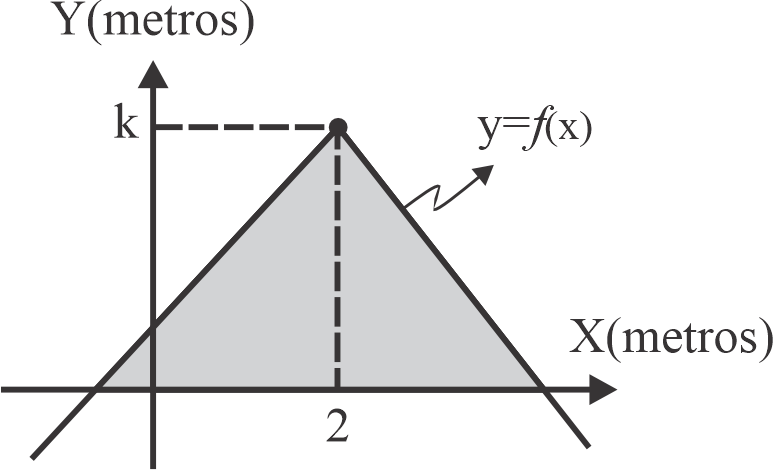
\includegraphics[width=4.5cm]{imagenes/CEPRE-UNA2024-I/etapa2/ing/alg1c24-I.png}
	\end{center}
	
	Halle el área de la región sombreada en metros cuadrados.
	
	\begin{enumerate}[label=\alph*)]
		\item $3\ m^2$
		\item $6\ m^2$
		\item $9\ m^2$
		\item $12\ m^2$
		\item $15\ m^2$
	\end{enumerate}
	\textbf{Respuesta correcta:} c)
	
	\vspace{2mm}
	\textbf{Solucionario:}
	
	$y-k=-|x-h|$ función valor absoluto que se abre hacia abajo.
	
	$\Rightarrow k=3$ y $h=2$.
	
	$|x-2|=-(y-3)$
	
	Si $y=0$:
	
	$\Rightarrow x=5 \quad \text{y} \quad x=-1$
	
	Entonces la base es:
	
	$5-(-1)=6$
	
	La altura es:
	
	$3$
	
	$A=\dfrac{6(3)}{2}=9\ m^2$
	
	\fbox{$A=9\ m^2$}
	
	\vspace{6mm}
	
	\item Halle el dominio de la función.
	
	$f(x)=\log_{4}\left[\log_{1/2}(\log_{3}x)\right]$
	
	\begin{enumerate}[label=\alph*)]
		\item $[-1;3]$
		\item $[1;3]$
		\item $\langle 1;3\rangle$
		\item $\langle 0;+\infty\rangle$
		\item $\langle 2;3\rangle$
	\end{enumerate}
	\textbf{Respuesta correcta:} c)
	
	\vspace{2mm}
	\textbf{Solucionario:}
	
	$\log_{1/2}(\log_3 x)>0$
	
	$\log_3 x<\left(\dfrac{1}{2}\right)^0$ y \quad $\log_3 x>0$
	
	$\log_3 x<1$ y \quad $x>1$
	
	$X<3$
	
	$\therefore \ D_f=\langle 1,3\rangle$
	
	\fbox{$D_f=\langle 1,3\rangle$}
	
	\vspace{6mm}
	
	\item Calcule el área del mayor rectángulo que tiene su base inferior en el eje $x$ y con dos vértices en la curva $y=12-x^2$
	
	\begin{enumerate}[label=\alph*)]
		\item $42\ u^2$
		\item $22\ u^2$
		\item $32\ u^2$
		\item $12\ u^2$
		\item $14\ u^2$
	\end{enumerate}
	\textbf{Respuesta correcta:} c)
	
	\vspace{2mm}
	\textbf{Solucionario:}
	
	\begin{tikzpicture}[scale=0.6, yscale=0.50]
		\draw[->, very thick] (-4,0) -- (4,0) node[right] {$x$};
		\draw[->, very thick] (0,-1) -- (0,13) node[above] {$y$};
		\draw[domain=-3.4:3.4,smooth,variable=\x,very thick] plot ({\x},{12-\x*\x});
		\draw[very thick] (-2,0) rectangle (2,8);
		\fill (2,8) circle (2.2pt) node[right] {$(x,y)$};
		\node at (0.6,12.5) {$12$};
		\node at (2,-0.45) {$2$};
	\end{tikzpicture}

	
	$A(x)=A=2x\cdot y=2x(12-x^2)$
	
	$A(x)=24x-2x^3$
	
	$A'(x)=24-6x^2 \Rightarrow x=2$
	
	$A''(x)=-12x$
	
	$A''(2)<0 \rightarrow A_{\max}(2)=32$
	
	\fbox{$A_{\max}=32\ u^2$}
	
	\vspace{6mm}
	
	\item Determine la variación de la expresión:
	
	$$E=\dfrac{x^2+y^2}{x^2+xy+y^2}, \quad \text{si } x,y\in \mathbb{R}^{+}$$
	
	\begin{enumerate}[label=\alph*)]
		\item $E\in \left[\dfrac{2}{3};1\right]$
		\item $E\in \left[\dfrac{2}{3};+\infty\right\rangle$
		\item $E\in \left[\dfrac{2}{3};1\right\rangle$
		\item $E\in \left\langle 0;\dfrac{2}{3}\right]$
		\item $E\in \left\langle \dfrac{2}{3};1\right\rangle$
	\end{enumerate}
	\textbf{Respuesta correcta:} c)
	
	\vspace{2mm}
	\textbf{Solucionario:}
	
	$x^2+y^2\geq 2xy$
	
	$3(x^2+y^2)\geq 2x^2+2xy+2y^2$
	
	$\dfrac{x^2+y^2}{x^2+xy+y^2}\geq \dfrac{2}{3}$
	
	Además, como $xy>0$:
	
	$x^2+xy+y^2>x^2+y^2$
	
	$\therefore 1>\dfrac{x^2+y^2}{x^2+xy+y^2}$
	
	$\therefore E\in \left[\dfrac{2}{3},1\right\rangle$
	
	\fbox{$E\in \left[\dfrac{2}{3},1\right\rangle$}
	
	\vspace{6mm}
	
\end{enumerate}





\subsection*{Geometría}

\begin{enumerate}[resume]
	
	\item En la figura, si $AB=5\sqrt{2}$, halle $x$.
	
	\begin{center}
		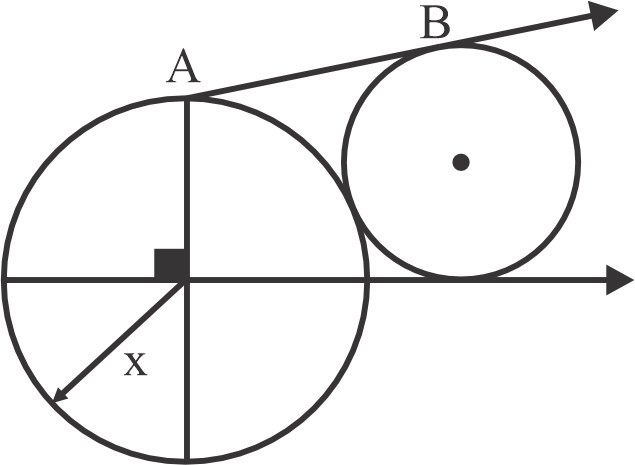
\includegraphics[width=4cm]{imagenes/CEPRE-UNA2024-I/etapa2/ing/geo1c24-I.png}
	\end{center}
	
	\begin{enumerate}[label=\alph*)]
		\item $\sqrt{2}$
		\item $3$
		\item $4$
		\item $5$
		\item $3\sqrt{2}$
	\end{enumerate}
	\textbf{Respuesta correcta:} d)
	
	\vspace{2mm}
	\textbf{Solucionario:}
	
	\begin{center}
		\begin{minipage}{0.45\textwidth}
		En el $\triangle AO'O$: por el teorema de Euclides.

		$(x+r)^2=\left(\sqrt{50+r^2}\right)^2+x^2-2x(x-r)$
		
		$x^2+2xr+r^2=50+r^2+x^2-2x^2+2xr$
		
		$2x^2=50$
		
		$x^2=25$
		
		$x=5$
		
		\fbox{$x=5$}
			\vspace{6mm}
		\end{minipage}
		\hfill
		\begin{minipage}{0.45\textwidth}
			\centering
			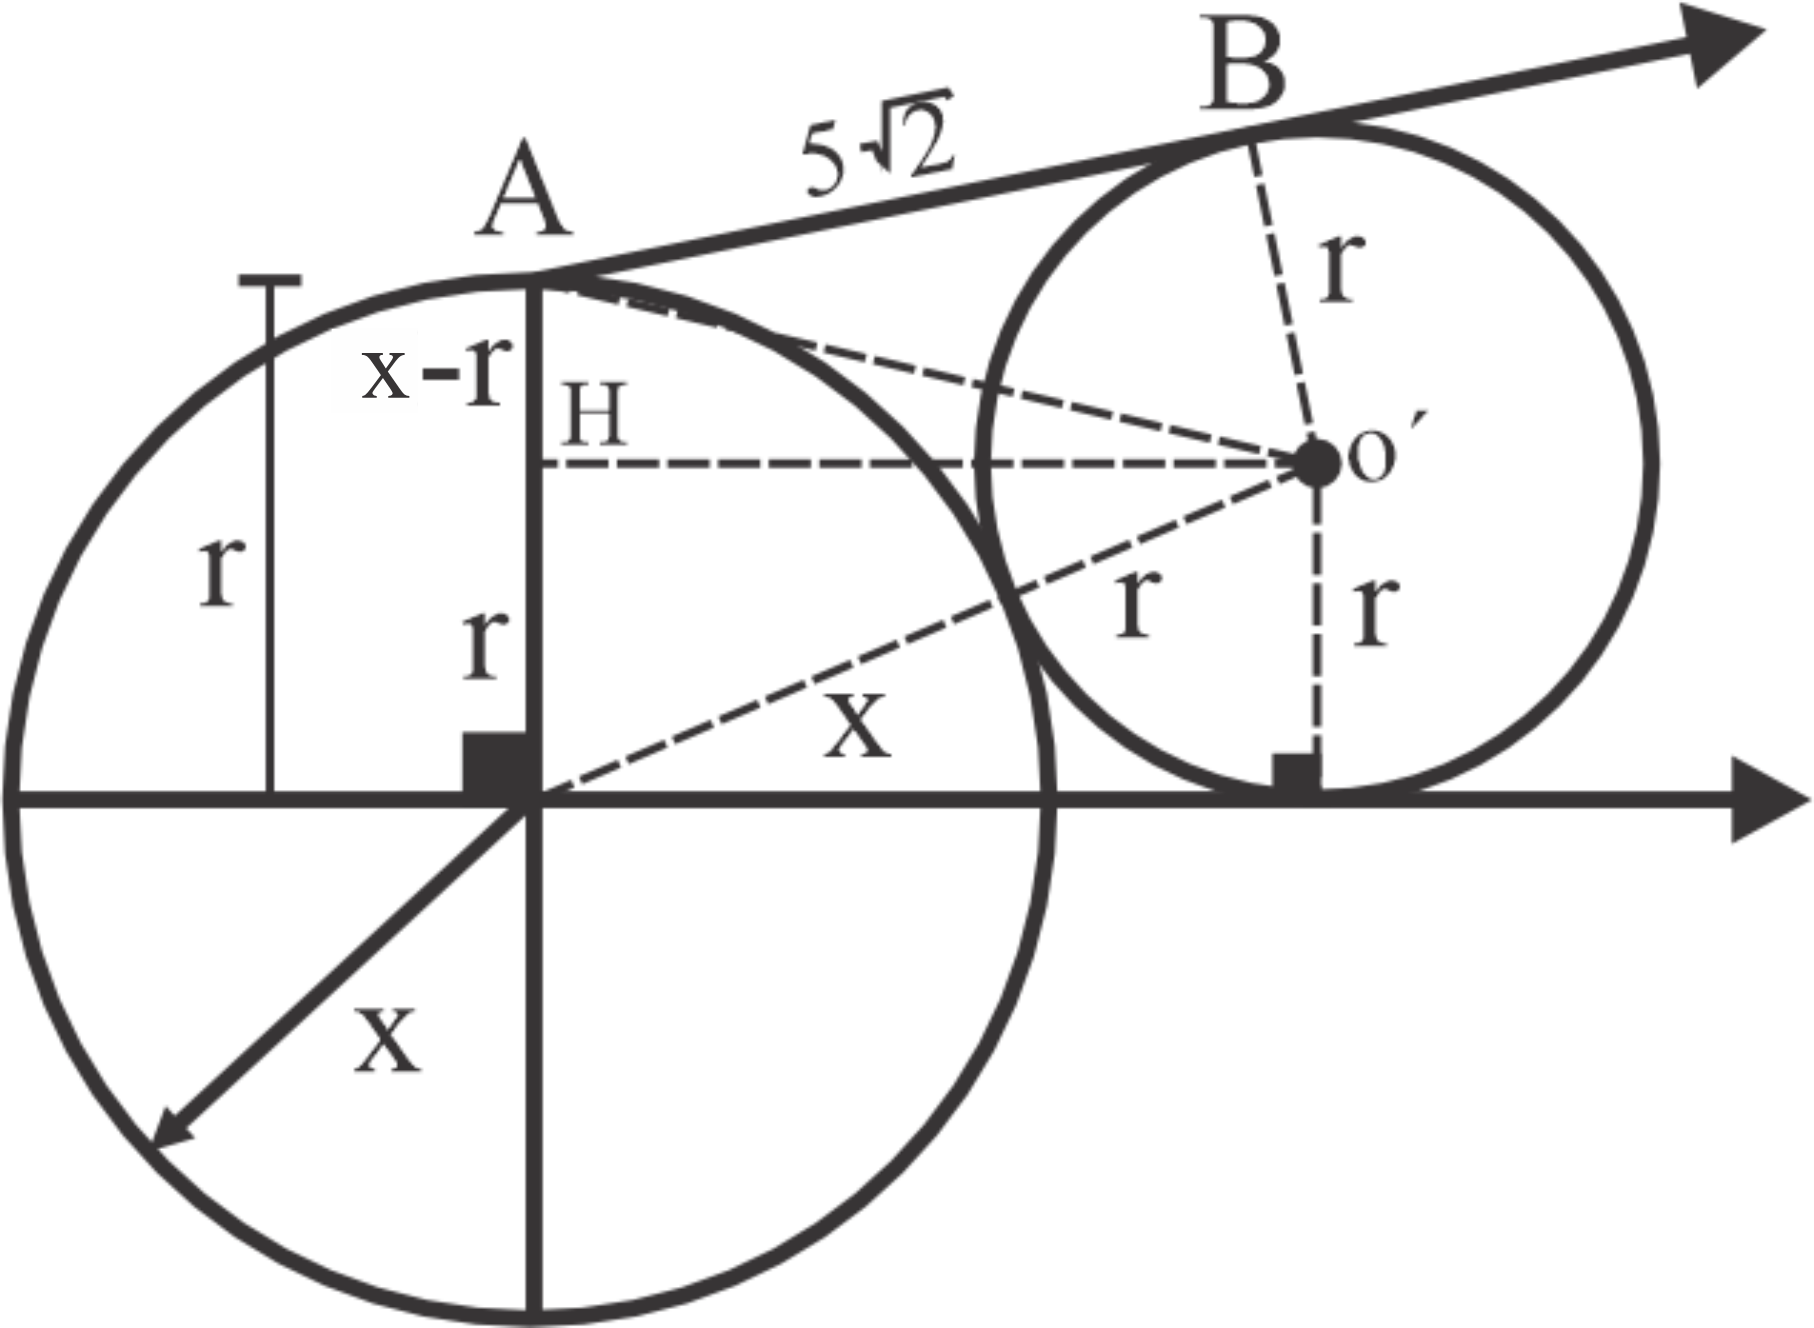
\includegraphics[width=4cm]{imagenes/CEPRE-UNA2024-I/etapa2/ing/geo1c24-Ir.png}
		\end{minipage}
	\end{center}
	
	
	
	\vspace{6mm}
	
	\item Roberto tiene una tabla en forma de triángulo equilátero, pero se da cuenta de que es demasiado grande, por lo que decide hacerle un corte para obtener un triángulo equilátero más pequeño. Calcule el perímetro de la tabla inicial.
	
	\begin{center}
		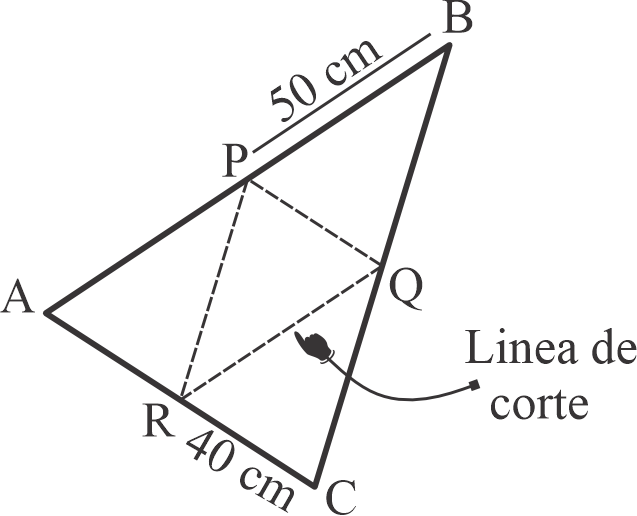
\includegraphics[width=4cm]{imagenes/CEPRE-UNA2024-I/etapa2/ing/geo2c24-I.png}
	\end{center}
	
	\begin{enumerate}[label=\alph*)]
		\item $210\ cm$
		\item $230\ cm$
		\item $250\ cm$
		\item $270\ cm$
		\item $280\ cm$
	\end{enumerate}
	\textbf{Respuesta correcta:} d)
	
	\vspace{2mm}
	\textbf{Solucionario:}
	
	
	
	
	\begin{center}
		\begin{minipage}{0.45\textwidth}
	
		Complemento ángulos, de donde:
		
		$\triangle APR\cong\triangle CRQ\cong\triangle BQP$ $(ALA)$
		
		Luego, $AR=CQ=PB=50\ cm$
		
		El lado del triángulo $\triangle ABC$ mide $90\ cm$
		
		Luego: perímetro $\triangle ABC=90+90+90$
		
		\fbox{$P_{\triangle ABC}=270\ cm$}
			\vspace{6mm}
		\end{minipage}
		\hfill
		\begin{minipage}{0.45\textwidth}
			\centering
			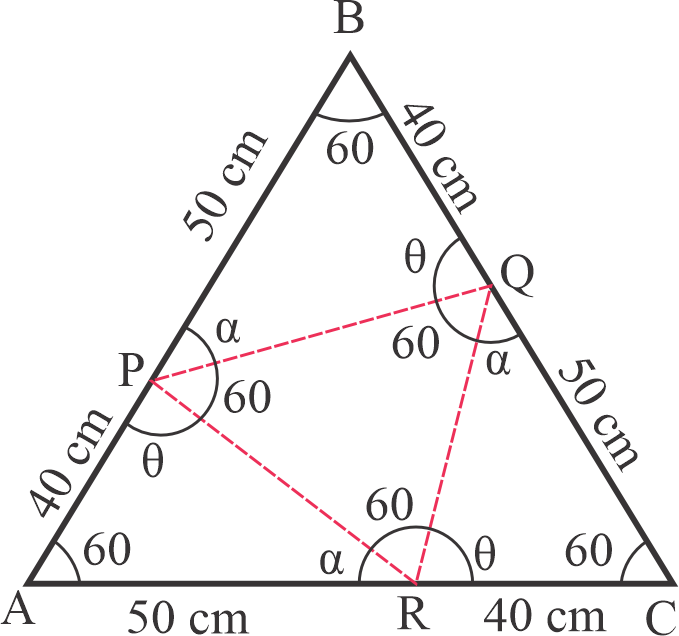
\includegraphics[width=4.2cm]{imagenes/CEPRE-UNA2024-I/etapa2/ing/geo2c24-Ir.png}
		\end{minipage}
	\end{center}
	
	
	
	
	
	
	\vspace{6mm}
	
	\item En la figura, calcule $x$.
	
	\begin{center}
		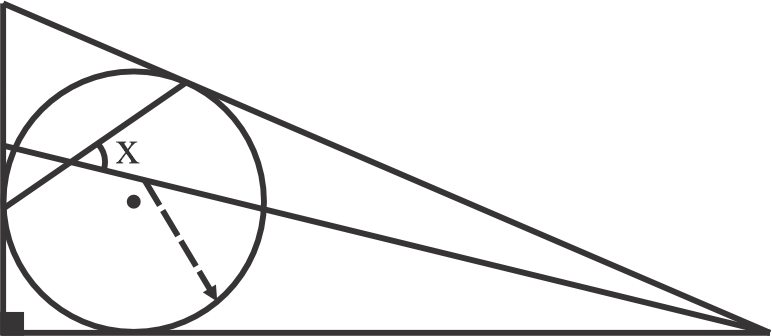
\includegraphics[width=5.2cm]{imagenes/CEPRE-UNA2024-I/etapa2/ing/geo3c24-I.png}
	\end{center}
	
	\begin{enumerate}[label=\alph*)]
		\item $60^\circ$
		\item $45^\circ$
		\item $83^\circ$
		\item $52^\circ$
		\item $74^\circ$
	\end{enumerate}
	\textbf{Respuesta correcta:} b)
	
	\vspace{2mm}
	\textbf{Solucionario:}

	
	\begin{center}
		\begin{minipage}{0.45\textwidth}
			
		En la figura obtenemos que:
		
		$\triangle MBC\cong\triangle MNC$ $(L.A.L)$
		
		
		$m\angle CMN=m\angle CMB=x$
		
		
		$m\angle MNA=m\angle MAB=\theta$
		
		$m\angle BPM=m\angle MNA=\theta$
		
		También del cuadrilátero $APMN$ obtendremos:
		
		$90^\circ+\theta+180^\circ-\theta+180^\circ-2x=360^\circ$
		
		$2x=90^\circ$
		
		
		\fbox{$x=45^\circ$}
			\vspace{6mm}
		\end{minipage}
		\hfill
		\begin{minipage}{0.45\textwidth}
			\centering
			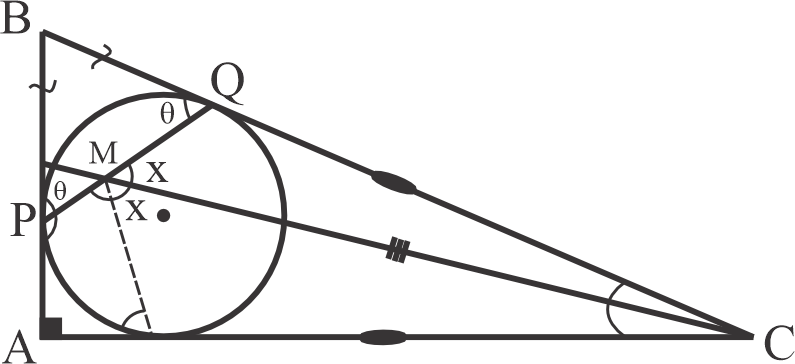
\includegraphics[width=5.2cm]{imagenes/CEPRE-UNA2024-I/etapa2/ing/geo3c24-Ir.png}
		\end{minipage}
	\end{center}
	
	
	
	
	\vspace{6mm}
	
	\item Se tiene dos conos de revolución en donde sus bases se encuentran en una mesa, y de altura $8\ m$ y $4\ m$ respectivamente. Un plano paralelo a la mesa intercepta a los dos conos a la misma altura, generando secciones equivalentes. Calcule el área de dicha sección en $m^2$.
	
	\begin{enumerate}[label=\alph*)]
		\item $12\pi\ m^2$
		\item $14\pi\ m^2$
		\item $16\pi\ m^2$
		\item $18\pi\ m^2$
		\item $25\pi\ m^2$
	\end{enumerate}
	\textbf{Respuesta correcta:} c)
	
	\vspace{2mm}
	\textbf{Solucionario:}
	
	Pide: $S'=$ área del círculo análogo.
	
	$i)$ Semejanza de triángulos en el cono 1:
	
	$\dfrac{r}{6}=\dfrac{8-a}{8}$
	
	$8r=48-6a$ \quad $\cdots (1)$
	
	$8r=24+4r$
	
	$4r=24-6a$
	
	$3a=12-r$ \quad $\cdots (2)$
	
	$ii)$ Semejanza de triángulos en el cono 2:
	
	$\dfrac{r}{12}=\dfrac{4-a}{4}$
	
	$4r=48-12a$
	
	$3a=12-r$ \quad $\cdots (3)$
	
	De $(1)$ y $(2)$:
	
	$12-r=24-4r$
	
	$3r=12$
	
	$r=4$
	
	Por lo tanto,
	
	$S'=\pi r^2=\pi(4)^2$
	
	\fbox{$S'=16\pi\ m^2$}
	
	\vspace{6mm}
	
\end{enumerate}





\subsection*{Trigonometría}

\begin{enumerate}[resume]
	
	\item Desde el pie de un poste, el ángulo de elevación de la punta de un campanario es $26^\circ 30'$, desde la parte superior del poste que tiene $10\ m$ de altura, el ángulo de elevación es $18^\circ 30'$. Halle la distancia entre el poste y el campanario.
	
	\begin{enumerate}[label=\alph*)]
		\item $30\ m$
		\item $60\ m$
		\item $50\ m$
		\item $42\ m$
		\item $45\ m$
	\end{enumerate}
	\textbf{Respuesta correcta:} b)
	
	\vspace{2mm}
	\textbf{Solucionario:}
	
	
	
	
		\begin{center}
		\begin{minipage}{0.45\textwidth}
			
		$18^\circ 30'=\left(\dfrac{\sqrt{37}}{2}\right)^\circ$\\
		
		
		$26^\circ 30'=\left(\dfrac{52}{2}\right)^\circ$\\

		$3x=2x+10$
		
		$x=10$
		
		distancia $=6x$
		
		$=6(10)$
		
		\fbox{$=60\ m$}
			\vspace{6mm}
		\end{minipage}
		\hfill
		\begin{minipage}{0.45\textwidth}
			\centering
			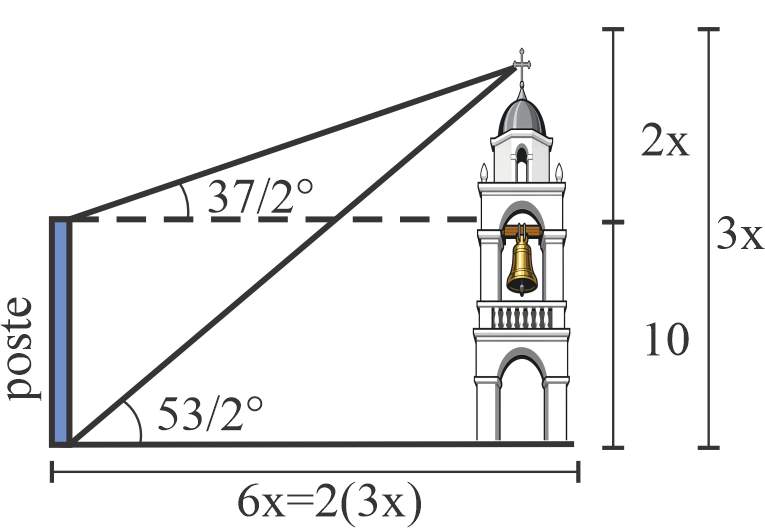
\includegraphics[width=5cm]{imagenes/CEPRE-UNA2024-I/etapa2/ing/trigo1c24-Ir.png}
		\end{minipage}
	\end{center}
	
	
	\vspace{6mm}
	
	\item En la figura, $ABCD$ es un rombo. Calcule $M=\tan\theta+\cot\theta$
	
	\begin{center}
		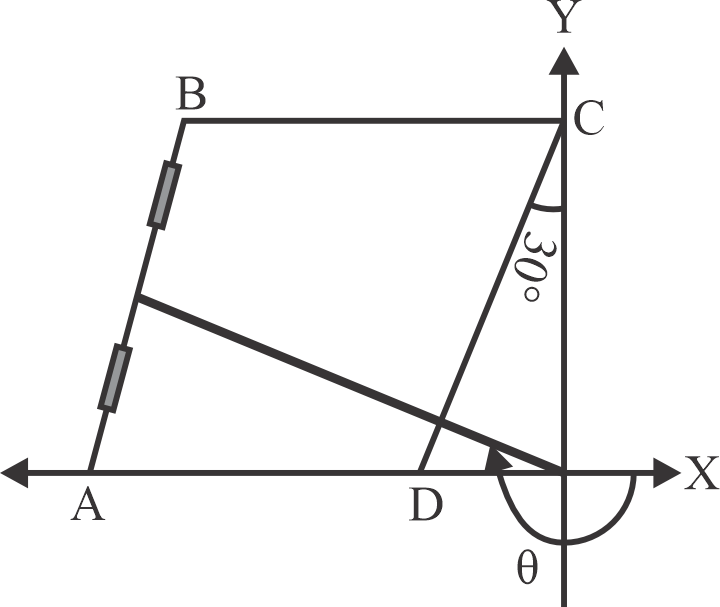
\includegraphics[width=4.8cm]{imagenes/CEPRE-UNA2024-I/etapa2/ing/trigo2c24-I.png}
	\end{center}
	
	\begin{enumerate}[label=\alph*)]
		\item $-\dfrac{25\sqrt{3}}{3}$
		\item $-\dfrac{8\sqrt{3}}{15}$
		\item $-\dfrac{20\sqrt{3}}{3}$
		\item $-\dfrac{28\sqrt{3}}{15}$
		\item $-\dfrac{28\sqrt{3}}{3}$
	\end{enumerate}
	\textbf{Respuesta correcta:} d)
	
	\vspace{2mm}
	\textbf{Solucionario:}
	
	
	\begin{center}
		\begin{minipage}{0.45\textwidth}
			
		$AB=BC=CD=AD$\\

		$\tan\theta+\cot\theta=-\dfrac{\sqrt{3}}{5}-\dfrac{5}{\sqrt{3}}$
		
		$=-\left(\dfrac{\sqrt{3}}{5}+\dfrac{5}{\sqrt{3}}\right)$\\
		
		$=-\left(\dfrac{3+25}{5\sqrt{3}}\right)$\\
		
		$=-\dfrac{28}{5\sqrt{3}}$
		
		\fbox{$\tan\theta+\cot\theta=-\dfrac{28\sqrt{3}}{15}$}
			\vspace{6mm}
		\end{minipage}
		\hfill
		\begin{minipage}{0.45\textwidth}
			\centering
			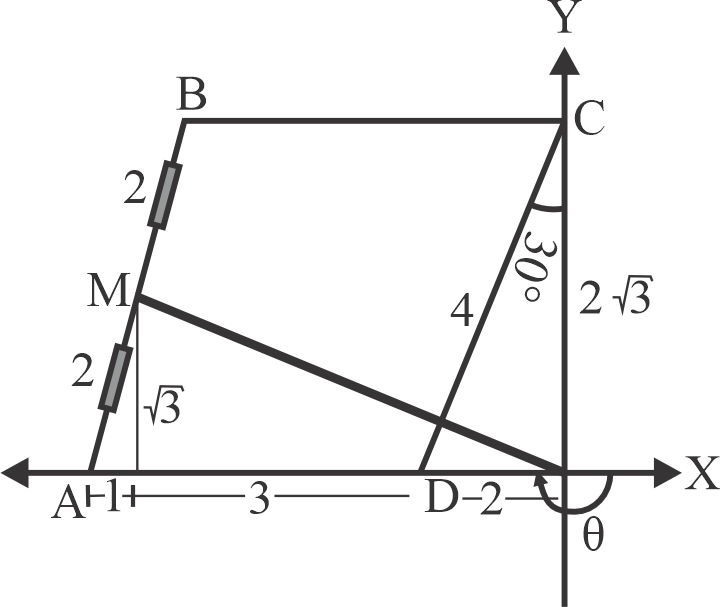
\includegraphics[width=4.8cm]{imagenes/CEPRE-UNA2024-I/etapa2/ing/trigo2c24-Ir.png}
		\end{minipage}
	\end{center}
	
	
	
	\vspace{6mm}
	
	\item Si $\theta\in\left[\dfrac{7\pi}{6},\dfrac{11\pi}{6}\right]$, determine la suma del máximo y mínimo valor de:
	
	$M=\sqrt{3}\cot\theta+3$
	
	\begin{enumerate}[label=\alph*)]
		\item $2$
		\item $3$
		\item $4$
		\item $5$
		\item $6$
	\end{enumerate}
	\textbf{Respuesta correcta:} e)
	
	\vspace{2mm}
	\textbf{Solucionario:}
	
	Analicemos en la circunferencia unitaria:
	
	$\theta\in\left[\dfrac{7\pi}{6},\dfrac{11\pi}{6}\right]\ ;\ \left[\dfrac{7\pi}{6},\dfrac{11\pi}{6}\right]=[210^\circ,330^\circ]$
	
	$\cot 210^\circ=\cot 30^\circ=\sqrt{3}$
	
	$\cot 330^\circ=-\cot 30^\circ=-\sqrt{3}$
	
	$210^\circ\leq \theta\leq 330^\circ$
	
	$\cot 210^\circ\geq \cot\theta\geq \cot 330^\circ$
	
	$\sqrt{3}\geq \cot\theta\geq -\sqrt{3}$
	
	$\sqrt{3}\cdot\sqrt{3}\geq \sqrt{3}\cot\theta\geq -\sqrt{3}(\sqrt{3})$
	
	$3\geq \sqrt{3}\cot\theta\geq -3$
	
	$3+3\geq \sqrt{3}\cot\theta+3\geq -3+3$
	
	$6\geq M\geq 0$
	
	Suma:
	
	\fbox{$6+0=6$}
	
	\vspace{6mm}
	
	\item A partir del triángulo $ABC$ de perímetro $30\ m$, reduzca la expresión:
	
	$M=(a+b)\cos C+(b+c)\cos A+(a+c)\cos B$
	
	\begin{enumerate}[label=\alph*)]
		\item $32\ m$
		\item $28\ m$
		\item $34\ m$
		\item $30\ m$
		\item $27\ m$
	\end{enumerate}
	\textbf{Respuesta correcta:} d)
	
	\vspace{2mm}
	\textbf{Solucionario:}
	
	
\begin{tikzpicture}[scale=0.6]
	
	% Vértices
	\coordinate (A) at (0,0);
	\coordinate (B) at (7,0);
	\coordinate (C) at (3.2,4.2);
	\coordinate (D) at (3.2,0);
	
	% Triángulo
	\draw[very thick] (A) -- (C) -- (B) -- cycle;
	
	% Altura
	\draw[very thick, red] (C) -- (D);
	
	% Etiquetas de lados
	\node[left] at ($(A)!0.55!(C)$) {$b$};
	\node[right] at ($(B)!0.55!(C)$) {$a$};
	\node[below] at ($(A)!0.25!(D)$) {$b\cos A$};
	\node[below] at ($(D)!0.5!(B)$) {$a\cos B$};
	\node[below] at ($(A)!0.5!(B)$) {$c$};
	
	% Ángulo recto
	\draw[very thick] ($(D)+(0,0.28)$) -- ($(D)+(0.28,0.28)$) -- ($(D)+(0.28,0)$);
	
	% Nombres de vértices
	\node[below left] at (A) {$A$};
	\node[below right] at (B) {$B$};
	\node[above] at (C) {$C$};
	
\end{tikzpicture}

	
	$c=b\cos A+a\cos B$
	
	$a=b\cos C+c\cos B$
	
	$b=a\cos C+c\cos A$
	
	$M=a\cos C+b\cos C+b\cos A+c\cos A+a\cos B+c\cos B$
	
	$=a\cos C+c\cos A+b\cos C+c\cos B+b\cos A+a\cos B$
	
	$=b+a+c$
	
	$=a+b+c$
	
	Como el perímetro del triángulo es $30\ m$:
	
	\fbox{$M=30\ m$}
	
	\vspace{6mm}
	
\end{enumerate}



\subsection*{Física}

\begin{enumerate}[resume]
	
	\item En la figura, halle el ángulo $\theta$ que determina el equilibrio de la barra homogénea que está sujeta a una cuerda de masa despreciable.
	
	\begin{center}
		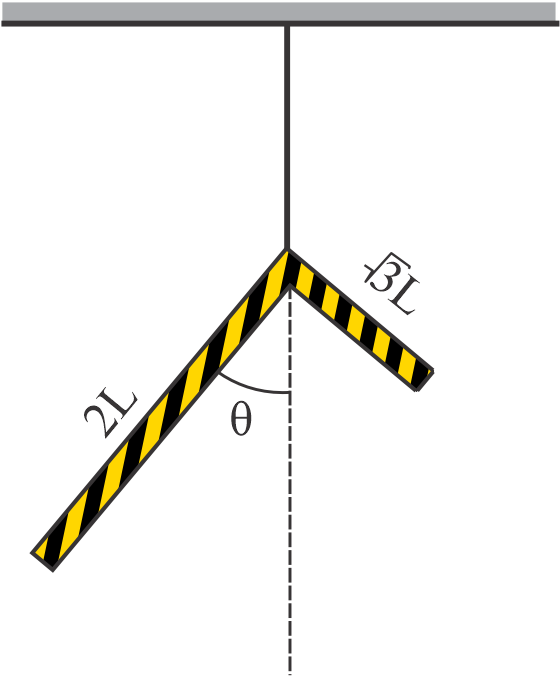
\includegraphics[width=2.8cm]{imagenes/CEPRE-UNA2024-I/etapa2/ing/fisica1c24-I.png}
	\end{center}
	
	
	\begin{enumerate}[label=\alph*)]
		\item $30^\circ$
		\item $37^\circ$
		\item $45^\circ$
		\item $53^\circ$
		\item $60^\circ$
	\end{enumerate}
	\textbf{Respuesta correcta:} b)
	
	\vspace{2mm}
	\textbf{Solucionario:}
	
	$M_1=M_2$
	
	$W_1d_1=W_2d_2$
	
	$k\,2L\cdot \sqrt{3}L\sen\theta=k\sqrt{3}L\cdot \dfrac{\sqrt{3}}{2}L\cos\theta$
	
	$\sen\theta=\dfrac{\sqrt{3}\sqrt{3}}{2(2)}\cos\theta$
	
	$\tan\theta=\dfrac{3}{4}$
	
	\fbox{$\theta=37^\circ$}
	
	\vspace{6mm}
	
	\item Determine la cantidad de calor necesario que se debe suministrar a $500\ g$ de hielo que se encuentra a $0^\circ C$ para convertirlo en agua a $20^\circ C$.
	
	\begin{enumerate}[label=\alph*)]
		\item $80\ \text{kcal}$
		\item $70\ \text{kcal}$
		\item $60\ \text{kcal}$
		\item $55\ \text{kcal}$
		\item $50\ \text{kcal}$
	\end{enumerate}
	\textbf{Respuesta correcta:} e)
	
	\vspace{2mm}
	\textbf{Solucionario:}
	
	$Q_t=Q_f+Q$
	
	$\Rightarrow L_f\,m+mc\,(T_f-T_i)$
	
	$\Rightarrow \left(80\dfrac{\text{cal}}{g}\right)(500\,g)+\left(500\,g\right)\left(1\dfrac{\text{cal}}{g^\circ C}\right)(20-0)^\circ C$
	
	$\Rightarrow (40000+10000)\,\text{cal}$
	
	$=50000\,\text{cal}=$\fbox{$50\,\text{kcal}$}
	
	\vspace{6mm}
	
	\item Una plancha eléctrica tiene una potencia de $800\ W$ cuando se conecta a una tensión de $220\ V$. Calcule su potencia de consumo a $110\ V$.
	
	\begin{enumerate}[label=\alph*)]
		\item $110\ W$
		\item $150\ W$
		\item $180\ W$
		\item $200\ W$
		\item $220\ W$
	\end{enumerate}
	\textbf{Respuesta correcta:} d)
	
	\vspace{2mm}
	\textbf{Solucionario:}
	
	$R_{(1)}=R_{(2)}$
	
	$\dfrac{V_1^2}{P_1}=\dfrac{V_2^2}{P_2}$
	
	$\dfrac{(220\,V)^2}{800}=\dfrac{(110)^2}{P_2}$
	
	$P_2=\dfrac{800(110)^2}{(220)^2}\,W$
	
	\fbox{$P_2=200\,W$}
	
	\vspace{6mm}
	
	\item ¿Con qué ángulo se refleja un rayo luminoso en un espejo plano que ha girado $15^\circ$ en sentido horario con respecto al rayo reflejado en el espejo en su posición original?
	
	\begin{enumerate}[label=\alph*)]
		\item $10^\circ$
		\item $20^\circ$
		\item $30^\circ$
		\item $40^\circ$
		\item $50^\circ$
	\end{enumerate}
	\textbf{Respuesta correcta:} c)
	
	\vspace{2mm}
	\textbf{Solucionario:}
	
	Nos piden hallar $\beta$
	
	$\theta_i+15^\circ+\theta_i+15^\circ=\theta_i+\theta_i+\beta$
	
	$2\theta_i+30^\circ=2\theta_i+\beta$
	
	\fbox{$30^\circ=\beta$}
	
	\vspace{6mm}
	
\end{enumerate}



\subsection*{Química}

\begin{enumerate}[resume]
	
	\item El increíble Hulk está jugando béisbol, batea una pelota cuya masa es $100\ g$, generando una longitud de onda $(\lambda)$ de $3{,}306\times10^{-26}\ \AA$. ¿A qué distancia llega la pelota en un tiempo de $3$ segundos?
	\begin{enumerate}[label=\alph*)]
		\item $5\ Km$
		\item $3\ Km$
		\item $60\ Km$
		\item $6\ Km$
		\item $400\ m$
	\end{enumerate}
	\textbf{Respuesta correcta:} d)
	
	\vspace{2mm}
	\textbf{Solucionario:}\\[1mm]
	
	$m=100\ g=10^2g\cdot\dfrac{1\ kg}{10^3g}=10^{-1}\ kg$
	
	$t=3\ s$
	
	$\lambda=3{,}306\times10^{-26}\ \AA\times\dfrac{10^{-10}\ m}{1\ \AA}=3{,}31\times10^{-36}\ m$
	
	$\lambda=\dfrac{h}{mu}$
	
	$u=\dfrac{h}{m\lambda}=\dfrac{6{,}62\times10^{-34}\ J\cdot s}{(10^{-1}\ kg)(3{,}31\times10^{-36}\ m)}$
	
	$u=\dfrac{6{,}62\times10^{-34}}{3{,}31\times10^{-37}}=2\times10^3\ \dfrac{m}{s}$
	
	$d=e=V\times t=(2\times10^3\ \dfrac{m}{s})(3\ s)=6\times10^3\ m$
	
	$=6\times10^3\ m\times\dfrac{1\ Km}{10^3\ m}=$\fbox{$6\ Km$}
	
	\vspace{6mm}
	
	\item ¿Cuál de los iones está mal nombrado?
	
	I. $\mathrm{ClO_4^-}$ Perclorato
	
	II. $\mathrm{PO_3^{3-}}$ Fosfato
	
	III. $\mathrm{CO_2^{2-}}$ Carbonato
	
	IV. $\mathrm{Cl^-}$ Cloruro
	
	V. $\mathrm{HSO_4^-}$ Bisulfato
	
	\begin{enumerate}[label=\alph*)]
		\item I y IV
		\item II y V
		\item Solo III
		\item IV y II
		\item Solo V
	\end{enumerate}
	\textbf{Respuesta correcta:} b)
	
	\vspace{2mm}
	\textbf{Solucionario:}\\[1mm]
	
	$(\mathrm{Cl^{+7}O_4^{2-}})^{1-}$ \quad perclorato \quad ok
	
	$(\mathrm{P^{+5}O_3^{2-}})^{1-}$ \quad fosfato \quad ok
	
	$(\mathrm{C^{+4}O_2^{2-}})$ \quad carbonato \quad no
	
	$\mathrm{Cl^{1-}}$ \qquad cloruro \quad ok
	
	$(\mathrm{H^{+1}S^{+6}O_4^{2-}})^{1-}$ \quad bisulfato \quad ok

	
	\vspace{6mm}
	
	\item Un gas ocupa un volumen de $1000\ mL$, a una temperatura de ``$X$'' $^\circ K$ y una presión de ``$P$'' atm. Si la presión disminuye a la mitad y la temperatura se duplica ¿qué volumen en mL ocupa el gas?
	\begin{enumerate}[label=\alph*)]
		\item $400$
		\item $4000$
		\item $4$
		\item $440$
		\item $800$
	\end{enumerate}
	\textbf{Respuesta correcta:} b)
	
	\vspace{2mm}
	\textbf{Solucionario:}\\[1mm]
	
	$V_1=1000\ mL$
	
	$T_1=X^\circ K$
	
	$P_1=P\ atm$
	
	$V_2=?$
	
	$T_2=2X^\circ K$
	
	$P_2=\dfrac{P}{2}\ atm$
	
	$\dfrac{P_1V_1}{T_1}=\dfrac{V_2P_2}{T_2}$
	
	$V_2=\dfrac{P_1V_1T_2}{P_2T_1}=\dfrac{(P)(1000\ mL)(2X)}{\left(\dfrac{P}{2}\right)X}$
	
	$V_2=4\times1000\ mL=$\fbox{$4000\ mL$}
	
	\vspace{6mm}
	
	\item El acetominofen es una amida usada para calmar el dolor; es decir como analgésico; y su estructura es:
	
	\begin{center}
		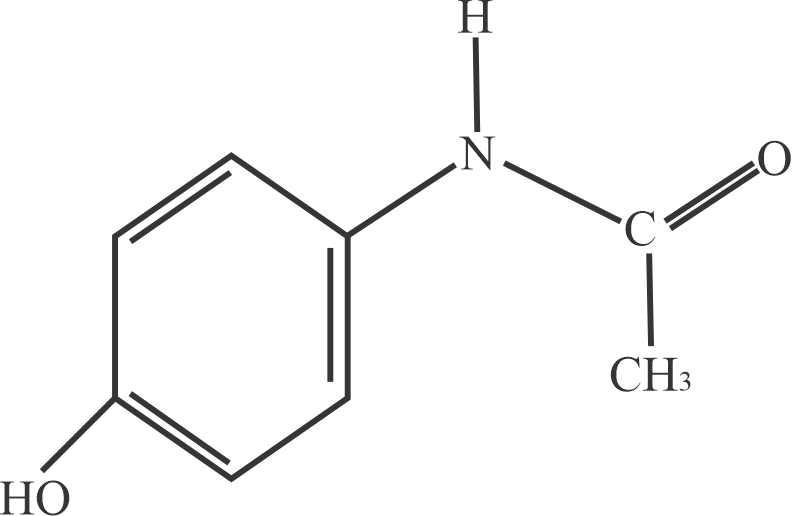
\includegraphics[width=4cm]{imagenes/CEPRE-UNA2024-I/etapa2/ing/quimica4c24-I.png}
	\end{center}
	
	Determine su peso molecular en g/mol
	\begin{enumerate}[label=\alph*)]
		\item $126$
		\item $96$
		\item $120$
		\item $151$
		\item $171$
	\end{enumerate}
	\textbf{Respuesta correcta:} d)
	
	\vspace{2mm}
	\textbf{Solucionario:}\\[1mm]
	
	$C=8\times12=96$
	
	$H=1\times9=9$
	
	$O=2\times16=32$
	
	$N=1\times14=14$
	
	$96+9+32+14=$\fbox{$151$}
	
	\vspace{6mm}
	
\end{enumerate}








\subsection*{Biología y Anatomía}

\begin{enumerate}[resume]
	
	\item El corazón tiene como función recibir y expulsar la sangre mediante los vasos sanguíneos. ¿Cuál es el vaso sanguíneo que sale del ventrículo derecho y transporta la sangre venosa hacia los pulmones?
	\begin{enumerate}[label=\alph*)]
		\item Vena cava superior
		\item Vena cava inferior
		\item Vena pulmonar
		\item Arteria pulmonar
		\item Arteria aorta
	\end{enumerate}
	\textbf{Respuesta correcta:} d)
	
	\vspace{2mm}
	\textbf{Solucionario:}\\[1mm]
	El vaso que lleva la sangre venosa hacia los pulmones es la \textbf{arteria pulmonar}.
	
	\vspace{6mm}
	
	\item Los mamíferos acuáticos respiran por:
	\begin{enumerate}[label=\alph*)]
		\item sacos pulmonares.
		\item branquias.
		\item vejiga natatoria.
		\item piel.
		\item pulmones.
	\end{enumerate}
	\textbf{Respuesta correcta:} e)
	
	\vspace{2mm}
	\textbf{Solucionario:}\\[1mm]
	Los mamíferos, aunque sean acuáticos, respiran por \textbf{pulmones}.
	
	\vspace{6mm}
	
\end{enumerate}

\subsection*{Psicología y Filosofía}

\begin{enumerate}[resume]

	
	\item Al comparar dos prendas, notamos una pequeña diferencia que da lugar a un cambio en la percepción. Este fenómeno se conoce como umbral:
	\begin{enumerate}[label=\alph*)]
		\item superior.
		\item mínimo.
		\item diferencial.
		\item máximo.
		\item sensorial.
	\end{enumerate}
	\textbf{Respuesta correcta:} c)
	
	\vspace{2mm}
	\textbf{Solucionario:}\\[1mm]
	La mínima diferencia perceptible entre dos estímulos se llama \textbf{umbral diferencial}.
	
	\vspace{6mm}
	
	\item Es el pensamiento multidireccional que se aplica en la solución del problema en muchas direcciones posibles. Se relaciona con la creatividad.
	\begin{enumerate}[label=\alph*)]
		\item Lógico
		\item No lógico
		\item Convergente
		\item Divergente
		\item Probabilístico
	\end{enumerate}
	\textbf{Respuesta correcta:} d)
	
	\vspace{2mm}
	\textbf{Solucionario:}\\[1mm]
	El pensamiento que explora varias posibilidades y alternativas es el \textbf{divergente}.
	
	\vspace{6mm}
	
	\item Juan, al terminar sus estudios universitarios, tendrá que sustentar su tesis. Esto implica que argumentará y explicará sus conclusiones con respecto a un tema. Entonces, su aprendizaje es:
	\begin{enumerate}[label=\alph*)]
		\item motor.
		\item actitudinal.
		\item social.
		\item instrumental.
		\item cognitivo.
	\end{enumerate}
	\textbf{Respuesta correcta:} e)
	
	\vspace{2mm}
	\textbf{Solucionario:}\\[1mm]
	Sustentar una tesis exige comprender, analizar, argumentar y explicar; eso corresponde al aprendizaje \textbf{cognitivo}.
	
	\vspace{6mm}
	
	\item El conocimiento científico es sistemático porque:
	
	\begin{enumerate}[label=\alph*)]
		\item cuestiona a otros conocimientos.
		\item consiste en una organización de leyes y teorías.
		\item está sujeto a un cambio constante.
		\item siempre problematiza sobre ciertos fenómenos.
		\item tiende a reflejar objetivamente la realidad.
	\end{enumerate}
	\textbf{Respuesta correcta:} b)
	
	\vspace{2mm}
	\textbf{Solucionario:}\\[1mm]
	Es sistemático porque organiza sus contenidos en un \textbf{conjunto ordenado de leyes y teorías}.
	
	\vspace{6mm}
	
\end{enumerate}

\subsection*{Geografía}

\begin{enumerate}[resume]

	
	\item Es la corriente marina que forma parte del proceso de circulación mayor del sector sur del Océano Pacífico y que se desplaza en sentido antihorario.
	\begin{enumerate}[label=\alph*)]
		\item Corriente Peruana
		\item Contracorriente Ecuatorial
		\item Corriente del Niño
		\item Corriente Australiana
		\item Corriente Cálida o Boreal
	\end{enumerate}
	\textbf{Respuesta correcta:} a)
	
	\vspace{2mm}
	\textbf{Solucionario:}\\[1mm]
	La corriente que integra la circulación del Pacífico Sur es la \textbf{Corriente Peruana}.
	
	\vspace{6mm}
	
	\item Es la parte visible dentro de la estructura solar de donde proviene la mayor parte de energía luminosa y calorífica que recibe la tierra:
	\begin{enumerate}[label=\alph*)]
		\item Corona
		\item Fotosfera
		\item Cabellera
		\item Núcleo
		\item Cromósfera
	\end{enumerate}
	\textbf{Respuesta correcta:} b)
	
	\vspace{2mm}
	\textbf{Solucionario:}\\[1mm]
	La parte visible del Sol es la \textbf{fotosfera}.
	
	\vspace{6mm}
	
\end{enumerate}

\subsection*{Historia}

\begin{enumerate}[resume]
	
	\item El Ministerio de Desarrollo e Inclusión Social, encargado de mejorar la calidad de vida de los peruanos en extrema pobreza y fomentar la equidad, proteger a poblaciones vulnerables y en estado de abandono, fue creado durante el gobierno de:
	\begin{enumerate}[label=\alph*)]
		\item Valentín Paniagua Corazao.
		\item Alberto Fujimori Fujimori.
		\item Alejandro Toledo Manrique.
		\item Fernando Belaunde Terry.
		\item Ollanta Humala Tasso.
	\end{enumerate}
	\textbf{Respuesta correcta:} e)
	
	\vspace{2mm}
	\textbf{Solucionario:}\\[1mm]
	El MIDIS fue creado durante el gobierno de \textbf{Ollanta Humala Tasso}.
	
	\vspace{6mm}
	
	\item Es la cultura que utilizó el barro, la quincha y el adobe en la arquitectura y cuya capital fue Cahuachi.
	\begin{enumerate}[label=\alph*)]
		\item Moche
		\item Chimú
		\item Paracas
		\item Tiahuanaco
		\item Nasca
	\end{enumerate}
	\textbf{Respuesta correcta:} e)
	
	\vspace{2mm}
	\textbf{Solucionario:}\\[1mm]
	Cahuachi fue el principal centro ceremonial de la cultura \textbf{Nasca}.
	
	\vspace{6mm}
	
\end{enumerate}

\subsection*{Educación Cívica}

\begin{enumerate}[resume]
	
	\item Durante la \rule{2cm}{0.4pt} se reconocen los derechos humanos de primera generación.
	\begin{enumerate}[label=\alph*)]
		\item creación de la ONU
		\item primera guerra mundial
		\item revolución francesa
		\item segunda guerra mundial
		\item revolución inglesa
	\end{enumerate}
	\textbf{Respuesta correcta:} c)
	
	\vspace{2mm}
	\textbf{Solucionario:}\\[1mm]
	Los derechos de primera generación se vinculan con la \textbf{Revolución francesa}.
	
	\vspace{6mm}
	
	\item En el testamento, se nombra a una persona natural o jurídica elegida por el testador para que cumpla o ejecute lo dispuesto en el documento. Se refiere:
	\begin{enumerate}[label=\alph*)]
		\item al tutor.
		\item al curador.
		\item al albacea.
		\item a los padrinos.
		\item a toda la familia.
	\end{enumerate}
	\textbf{Respuesta correcta:} c)
	
	\vspace{2mm}
	\textbf{Solucionario:}\\[1mm]
	La persona encargada de ejecutar lo dispuesto en el testamento es el \textbf{albacea}.
	
	\vspace{6mm}
	
\end{enumerate}

\subsection*{Economía}

\begin{enumerate}[resume]
	
	\item ¿Qué escuela económica sostiene que la riqueza de una nación está determinada por la cantidad de oro y plata que posee?
	\begin{enumerate}[label=\alph*)]
		\item Monetarista
		\item Keynesiana
		\item Neoclásica
		\item Mercantilista
		\item Socialista
	\end{enumerate}
	\textbf{Respuesta correcta:} d)
	
	\vspace{2mm}
	\textbf{Solucionario:}\\[1mm]
	La escuela que identifica la riqueza con la acumulación de metales preciosos es la \textbf{mercantilista}.
	
	\vspace{6mm}
	
	\item En la apertura de un mercado de abastos en la ciudad de Puno, participaron gran número de vendedores, debido a la inclemencia del tiempo hubo un solo comprador. ¿A qué tipo de mercado de competencia corresponde?
	\begin{enumerate}[label=\alph*)]
		\item Mercado mixto
		\item Mercado de capitales
		\item Mercado de monopolio
		\item Mercado de oligopolio
		\item Mercado de monopsonio
	\end{enumerate}
	\textbf{Respuesta correcta:} e)
	
	\vspace{2mm}
	\textbf{Solucionario:}\\[1mm]
	Muchos vendedores y un solo comprador corresponden a un \textbf{monopsonio}.
	
	\vspace{6mm}
	
\end{enumerate}

\subsection*{Comunicación}

\begin{enumerate}[resume]
	
	\item Una oración contiene sujeto y predicado. El sujeto identifica al ser u objeto. El predicado expresa la acción o estado del ser u objeto. El enunciado utiliza el lenguaje en su función:
	\begin{enumerate}[label=\alph*)]
		\item metalingüística.
		\item fática o de contacto.
		\item apelativa o conativa.
		\item referencial o representativa.
		\item expresiva o emotiva.
	\end{enumerate}
	\textbf{Respuesta correcta:} a)
	
	\vspace{2mm}
	\textbf{Solucionario:}\\[1mm]
	El enunciado habla sobre la estructura de la oración y explica elementos del propio lenguaje; por eso cumple función \textbf{metalingüística}.
	
	\vspace{6mm}
	
	\item El transbordador espacial es una estructura de aluminio cubierto de un sistema aislante que impide que temperaturas mayores a $177^\circ C$ se registren dentro del armazón de aluminio y de la fibra de vidrio. El costo de este tipo de cubierta es de un poco más de $23,7$ metros; y el área total es de $250$ metros cuadrados. El fragmento corresponde a un texto:
	\begin{enumerate}[label=\alph*)]
		\item narrativo.
		\item descriptivo.
		\item argumentativo.
		\item instructivo.
		\item dialógico.
	\end{enumerate}
	\textbf{Respuesta correcta:} b)
	
	\vspace{2mm}
	\textbf{Solucionario:}\\[1mm]
	Presenta características y rasgos de un objeto; por ello es un texto \textbf{descriptivo}.
	
	\vspace{6mm}
	
	\item La cohesión es una propiedad textual que se distingue de las demás porque se centra en el aspecto:
	\begin{enumerate}[label=\alph*)]
		\item sintáctico que ve como una frase u oración se conecta lingüísticamente con otra frase u oración.
		\item semántico que ve como la información se distribuye según el esquema global del texto.
		\item pragmático que ve como se seleccionan las estructuras lingüísticas en función de los componentes relacionales.
		\item intencional que ve el motivo que impulsa el desarrollo del texto en una situación comunicativa concreta.
		\item referencial que ve el modo como la realidad se conecta con la expresión lingüística.
	\end{enumerate}
	\textbf{Respuesta correcta:} a)
	
	\vspace{2mm}
	\textbf{Solucionario:}\\[1mm]
	La cohesión se refiere a los enlaces formales entre oraciones; por eso se centra en el aspecto \textbf{sintáctico}.
	
	\vspace{6mm}
	
	\item Juanita tiene 12 años y, en las mañanas, lava los platos y ayuda a su madre en la cocina. El enunciado utiliza el lenguaje en su función:
	\begin{enumerate}[label=\alph*)]
		\item referencial o representativa.
		\item expresiva o emotiva.
		\item apelativa o conativa.
		\item fática y de contacto.
		\item metalingüística.
	\end{enumerate}
	\textbf{Respuesta correcta:} a)
	
	\vspace{2mm}
	\textbf{Solucionario:}\\[1mm]
	El enunciado brinda información objetiva sobre Juanita; por tanto, la función es \textbf{referencial}.
	
	\vspace{6mm}
	
\end{enumerate}

\subsection*{Literatura}

\begin{enumerate}[resume]
	
	\item Es una característica distintiva de la novela \textit{Cien Años de Soledad} de Gabriel García Márquez.
	\begin{enumerate}[label=\alph*)]
		\item Está narrada en primera persona.
		\item Mezcla la lírica con la prosa.
		\item Uso de un lenguaje prosáico.
		\item Es un gran monólogo interior.
		\item Emplea el tiempo narrativo cíclico.
	\end{enumerate}
	\textbf{Respuesta correcta:} e)
	
	\vspace{2mm}
	\textbf{Solucionario:}\\[1mm]
	Una característica central de la novela es el \textbf{tiempo narrativo cíclico}.
	
	\vspace{6mm}
	
	\item En el cuento \textit{El Caballero Carmelo}, Carmelo era un gallo:
	\begin{enumerate}[label=\alph*)]
		\item bravucón y necio.
		\item luchador pero ridículo.
		\item viejo y achacoso.
		\item furioso y conciliador.
		\item de alcurnia y galante.
	\end{enumerate}
	\textbf{Respuesta correcta:} c)
	
	\vspace{2mm}
	\textbf{Solucionario:}\\[1mm]
	El Caballero Carmelo es presentado como un gallo \textbf{viejo y achacoso}.
	
	\vspace{6mm}
	
\end{enumerate}

\subsection*{Razonamiento Matemático}

\begin{enumerate}[resume]
	
	\item Juan le regala a su hijo Pedro la suma de:
	
	$C=12_{(3)}+23_{(4)}+34_{(5)}+45_{(6)}+\cdots$
	
	$10$ sumandos
	
	Halle dicha cantidad en el sistema decimal.
	\begin{enumerate}[label=\alph*)]
		\item $560$
		\item $561$
		\item $570$
		\item $575$
		\item $580$
	\end{enumerate}
	\textbf{Respuesta correcta:} a)
	
	\vspace{2mm}
	\textbf{Solucionario:}


	Analizamos la forma de cada término de la serie ($T_k$):
	\begin{itemize}
		\item $T_1 = 12_{(3)} = 1(3) + 2 = 5$
		\item $T_2 = 23_{(4)} = 2(4) + 3 = 11$
		\item $T_3 = 34_{(5)} = 3(5) + 4 = 19$
	\end{itemize}
	
	$ T_k = k(k+2) + (k+1) $
	
	$ T_k = k^2 + 2k + k + 1 = k^2 + 3k + 1 $
	
	$ C = \sum_{k=1}^{10} (k^2 + 3k + 1) $
	
	$ C = \sum_{k=1}^{10} k^2 + 3\sum_{k=1}^{10} k + \sum_{k=1}^{10} 1 $
	
	Aplicando las fórmulas de sumas notables:
	\begin{enumerate}
		\item Suma de cuadrados: $\dfrac{10(11)(21)}{6} = 385$
		\item Suma de naturales: $3 \times \dfrac{10(11)}{2} = 3(55) = 165$
		\item Suma de constantes: $1 \times 10 = 10$
	\end{enumerate}
	

	$C = 385 + 165 + 10 =$\fbox{$560$}
	
	\vspace{6mm}
	
	\item En cierto año ocurrió que el primer día de un determinado mes fue lunes, mientras que el último día de dicho mes también fue lunes. ¿Qué fecha cayó el primer jueves del mes posterior?
	\begin{enumerate}[label=\alph*)]
		\item 3 de marzo
		\item 2 de mayo
		\item 4 de marzo
		\item 30 de abril
		\item 24 de junio
	\end{enumerate}
	\textbf{Respuesta correcta:} a)
	
	\vspace{2mm}
	\textbf{Solucionario:}
	
	Si el primer día y el último día de un mes son lunes, entonces el mes tiene $29$ días.
	
	El mes siguiente comienza un martes.
	
	Por tanto, el primer jueves del mes siguiente cae el día:

	
	\fbox{$3$ de marzo}
	
	\vspace{6mm}
	
	\item En el gráfico, $T$ y $P$ son puntos de tangencia. Si $AB=2$, calcule el área de la región sombreada.
	
	\begin{center}
		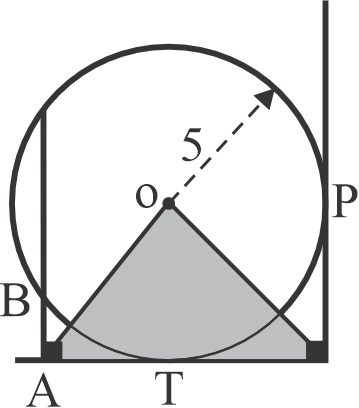
\includegraphics[width=3cm]{imagenes/CEPRE-UNA2024-I/etapa2/ing/rm3c24-I.png}
	\end{center}
	
	\begin{enumerate}[label=\alph*)]
		\item $20\ u^2$
		\item $\dfrac{45}{2}\ u^2$
		\item $25\ u^2$
		\item $\dfrac{49}{2}\ u^2$
		\item $21\ u^2$
	\end{enumerate}
	\textbf{Respuesta correcta:} b)
	
	\vspace{2mm}
	\textbf{Solucionario:}\\[1mm]
	Del gráfico, el radio del círculo es $5$.
	
	Como $AB=2$, en el triángulo rectángulo formado con el radio:
	
	$x^2+3^2=5^2$
	
	$x^2+9=25$
	
	$x=4$
	
	Entonces la base total del triángulo sombreado es:
	
	$AO=AT+TO=4+5=9$
	
	y su altura es el radio:
	
	$5$
	
	Área sombreada:
	
	$A=\dfrac{9\cdot5}{2}=\dfrac{45}{2}\ u^2$
	
	\fbox{$\dfrac{45}{2}\ u^2$}
	
	\vspace{6mm}
	
	\item Se divide un terreno rectangular en parcelas lográndose $108$ parcelas cuadradas de $121\ m^2$ cada una. En cada esquina de las parcelas se coloca un poste, empleándose en total $130$ postes. Halle la diferencia entre el largo y el ancho del terreno rectangular.
	\begin{enumerate}[label=\alph*)]
		\item $44\ m$
		\item $33\ m$
		\item $38\ m$
		\item $52\ m$
		\item $50\ m$
	\end{enumerate}
	\textbf{Respuesta correcta:} b)
	
	\vspace{2mm}
	\textbf{Solucionario:}\\[1mm]
	Cada parcela tiene lado:
	
	$\sqrt{121}=11\ m$
	
	Si el rectángulo tiene $m$ parcelas por un lado y $n$ por el otro:
	
	$mn=108$
	
	y el número de postes es:
	
	$(m+1)(n+1)=130$
	
	$mn+m+n+1=130$
	
	$108+m+n+1=130$
	
	$m+n=21$
	
	Los números que cumplen:
	
	$m=9,\quad n=12$
	
	La diferencia de dimensiones es:
	
	$(12-9)\cdot 11=33\ m$
	
	\fbox{$33\ m$}
	
	\vspace{6mm}
	
	\item Calcule la suma de los 10 primeros términos de la serie
	
	$S=4+12+26+46+\cdots$
	\begin{enumerate}[label=\alph*)]
		\item $1200$
		\item $1110$
		\item $1320$
		\item $1120$
		\item $1000$
	\end{enumerate}
	\textbf{Respuesta correcta:} d)
	
	\vspace{2mm}
	\textbf{Solucionario:}\\[1mm]
	Las diferencias son:
	
	$8,\ 14,\ 20,\dots$
	
	La segunda diferencia es constante, entonces:
	
	$a_n=3n^2-n+2$
	
	Luego:
	
	$S_{10}=\sum_{n=1}^{10}(3n^2-n+2)$
	
	$=3\sum_{n=1}^{10}n^2-\sum_{n=1}^{10}n+2\sum_{n=1}^{10}1$
	
	$=3(385)-55+20$
	
	$=1155-55+20$
	
	\fbox{$= 1120$}
	
	\vspace{6mm}
	
	\item Halle la suma de los elementos de la matriz $10\times10$
	
	\[
	\begin{bmatrix}
		2 & 4 & 6 & \cdots & 18 & 20\\
		4 & 6 & 8 & \cdots & 20 & 22\\
		6 & 8 & 10 & \cdots & 22 & 24\\
		\vdots & \vdots & \vdots & \ddots & \vdots & \vdots\\
		20 & 22 & 24 & \cdots & 36 & 38
	\end{bmatrix}
	\]
	
	\begin{enumerate}[label=\alph*)]
		\item $2200$
		\item $2100$
		\item $2580$
		\item $2000$
		\item $2700$
	\end{enumerate}
	\textbf{Respuesta correcta:} d)
	
	\vspace{2mm}
	\textbf{Solucionario:}\\[1mm]
	El término general es:
	
	$a_{ij}=2(i+j-1)$
	
	Entonces:
	
	$\displaystyle \sum_{i=1}^{10}\sum_{j=1}^{10} a_{ij}
	=\sum_{i=1}^{10}\sum_{j=1}^{10}2(i+j-1)$
	
	$=2\left(10\sum_{i=1}^{10}i+10\sum_{j=1}^{10}j-100\right)$
	
	$=2(10\cdot55+10\cdot55-100)$
	
	$=2(550+550-100)$
	
	$=2(1000)=2000$
	
	\fbox{$2000$}
	
	\vspace{6mm}
	
\end{enumerate}

\subsection*{Razonamiento Verbal}

\begin{enumerate}[resume]
	
	\item Marque la relación incorrecta de sustantivos colectivos:
	\begin{enumerate}[label=\alph*)]
		\item pinar : pinos
		\item clientela : clientes
		\item bosque : árboles
		\item estrellada : estrellas
		\item dentadura : dientes
	\end{enumerate}
	\textbf{Respuesta correcta:} d)
	
	\vspace{2mm}
	\textbf{Solucionario:}\\[1mm]
	``Estrellada'' no es un sustantivo colectivo de estrellas.
	
	La relación incorrecta es:
	
	\fbox{estrellada : estrellas}
	
	\vspace{6mm}
	
	\item La palabra que está implicada en las demás es:
	\begin{enumerate}[label=\alph*)]
		\item legislación.
		\item reglamento.
		\item normativa.
		\item ordenanza.
		\item estatuto.
	\end{enumerate}
	\textbf{Respuesta correcta:} c)
	
	\vspace{2mm}
	\textbf{Solucionario:}\\[1mm]
	La palabra más general, que engloba a las demás, es \textbf{normativa}.
	
	\vspace{6mm}
	
	\item En las oraciones ``Estamos en una estación, en la que los árboles comienzan a florecer y los días se vuelven más largos'' y ``El tren llegó a la estación a tiempo para recoger a los pasajeros que se dirigían a la ciudad''.
	
	¿Cuál es la relación entre las palabras subrayadas?
	\begin{enumerate}[label=\alph*)]
		\item Paronimia
		\item Homografía
		\item Homofonía
		\item Polisemia
		\item Homonimia
	\end{enumerate}
	\textbf{Respuesta correcta:} d)
	
	\vspace{2mm}
	\textbf{Solucionario:}\\[1mm]
	La palabra ``estación'' tiene varios significados relacionados entre sí; eso es \textbf{polisemia}.
	
	\vspace{6mm}
	
	\item El antónimo de la palabra VITUPERABLE es:
	\begin{enumerate}[label=\alph*)]
		\item censurable.
		\item reprochable.
		\item laudable.
		\item condenable.
		\item recusable.
	\end{enumerate}
	\textbf{Respuesta correcta:} c)
	
	\vspace{2mm}
	\textbf{Solucionario:}\\[1mm]
	``Vituperable'' significa digno de reproche; su antónimo es \textbf{laudable}.
	
	\vspace{6mm}
	
	\item PLAN DE REDACCIÓN
	
	Las plantas de interior
	
	I. Hay condiciones ambientales para promover su eficaz desarrollo.
	
	II. Existen diversos tipos de plantas de interior.
	
	III. Su principal función consiste en ser objeto de ornato.
	
	IV. Una de ellas es la adecuada iluminación y
	
	V. Las hay desde las más modestas hasta las más exóticas.
	
	\begin{enumerate}[label=\alph*)]
		\item III -- V -- I -- IV -- II
		\item II -- I -- V -- IV -- III
		\item II -- III -- V -- I -- IV
		\item II -- V -- III -- I -- IV
		\item III -- II -- V -- I -- IV
	\end{enumerate}
	\textbf{Respuesta correcta:} d)
	
	\vspace{2mm}
	\textbf{Solucionario:}\\[1mm]
	Primero se presenta el tema general: II.
	
	Luego se amplía la variedad de las plantas: V.
	
	Después se señala su función principal: III.
	
	Finalmente se mencionan las condiciones para su desarrollo: I, y se precisa una de ellas: IV.
	
	Orden:
	
	II -- V -- III -- I -- IV
	
	\vspace{6mm}
	
	\item Siempre que tomo café en las tardes, no puedo dormir esa noche. Si lo tomo por la mañana, no podré conciliar el sueño hasta medianoche. ¿Cuál de las opciones es necesariamente cierta?
	\begin{enumerate}[label=\alph*)]
		\item Son las dos de la mañana y estoy despierto. Hoy he tomado café.
		\item Tomé café en el desayuno. A las dos de la mañana estaré despierto.
		\item Son las once de la noche y estoy dormido. Hoy no he tomado café.
		\item Estoy despierto a las doce y media de la noche. Hoy he tomado café por la mañana.
		\item Tomé café por la tarde. Dormiré a la medianoche.
	\end{enumerate}
	\textbf{Respuesta correcta:} c)
	
	\vspace{2mm}
	\textbf{Solucionario:}\\[1mm]
	Si toma café en la tarde, no duerme esa noche.
	
	Si lo toma en la mañana, no duerme hasta medianoche.
	
	Entonces, si a las once de la noche está dormido, necesariamente \textbf{no tomó café ese día}.
	
	\vspace{6mm}
\end{enumerate}

\subsection*{Inglés}

\begin{enumerate}[resume]
	
	\item Find the list with the right question words to complete the questions of this conversation.
	
	A: Good morning, sir. \rule{1.5cm}{0.4pt} is your name?
	
	B: My name is Brown.
	
	A: \rule{1.5cm}{0.4pt} did you arrive?
	
	B: At 8:00 o'clock this morning.
	
	A: \rule{1.5cm}{0.4pt} did you come here?
	
	B: I took a taxi.
	
	\begin{enumerate}[label=\alph*)]
		\item What -- Who -- Where
		\item What -- How -- Who
		\item What -- When -- How
		\item What -- Who -- When
		\item What -- Where -- How
	\end{enumerate}
	\textbf{Respuesta correcta:} c)
	
	\vspace{2mm}
	\textbf{Solucionario:}\\[1mm]
	Las preguntas correctas son:
	
	What is your name?
	
	When did you arrive?
	
	How did you come here?
	
	\vspace{6mm}
	
	\item Look at this chart, and choose the right information
	
\begin{center}
	\begin{tikzpicture}
		% marco
		\draw[thick] (0,0) rectangle (9.5,6.6);
		
		% columnas
		\draw[thick] (2.6,0) -- (2.6,6.6);
		\draw[thick] (5.9,0) -- (5.9,6.6);
		
		% filas
		\draw[thick] (0,5.5) -- (9.5,5.5);
		\draw[thick] (0,3.7) -- (9.5,3.7);
		\draw[thick] (0,1.9) -- (9.5,1.9);
		
		% encabezados
		\node at (1.3,6.05) {Name};
		\node at (4.25,6.05) {is going to};
		\node at (7.7,6.05) {isn't going to ...};
		
		% Susan
		\node at (1.3,4.6) {Susan};
		\node at (4.25,4.95) {build};
		\node at (4.25,4.55) {a};
		\node at (4.25,4.15) {bridge};
		\node at (7.7,4.25) {build a house};
		
		% Hanna
		\node at (1.3,2.8) {Hanna};
		\node at (4.25,3.1) {study};
		\node at (4.25,2.6) {English};
		\node at (7.7,2.8) {build a road};
		
		% Simon
		\node at (1.3,0.95) {Simon};
		\node at (4.25,1.35) {build};
		\node at (4.25,0.95) {a};
		\node at (4.25,0.55) {bridge};
		\node at (7.7,0.95) {study English};
	\end{tikzpicture}
\end{center}

	\begin{enumerate}[label=\alph*)]
		\item Susan and Simon are going to build a bridge.
		\item Hanna is going to build a road.
		\item Simon and Susan are going to study English.
		\item Susan and Hanna are going to build a house.
		\item Simon is going to build a road.
	\end{enumerate}
	\textbf{Respuesta correcta:} a)
	
	\vspace{2mm}
	\textbf{Solucionario:}\\[1mm]
	Según la tabla, Susan is going to build a bridge y Simon is going to build a bridge.
	
	Por tanto, la opción correcta es:
	
	\fbox{Susan and Simon are going to build a bridge.}
	
	\vspace{6mm}
	
\end{enumerate}

\subsection*{Quechua y Aimara}

\begin{enumerate}[resume]
	
	\item ¿Pikunatataq puñunapiri puñunku?/¿Khitinakasa ikinana ikipxi?
	\begin{enumerate}[label=\alph*)]
		\item Uywakuna / Uywanaka
		\item Allqukuna / Anunaka
		\item Pichinkukuna / Jamach'inaka
		\item Runakuna / Jaqinaka
		\item Khuchikuna / Khuchinaka
	\end{enumerate}
	\textbf{Respuesta correcta:} d)
	
	\vspace{2mm}
	\textbf{Solucionario:}\\[1mm]
	``Pikunatataq'' y ``Khitinakasa'' se refieren a \textbf{quiénes}; por tanto corresponde \textbf{personas}.
	
	Quechua: runakuna
	
	Aimara: jaqinaka
	
	\vspace{6mm}
	
	\item ¿Imatataq misikunari mikhunku?/¿Kunsa phisinakaxa manq'apxi?
	\begin{enumerate}[label=\alph*)]
		\item Q'achuta / Chuxlla
		\item Yakuta / Uma
		\item Alpata / Laq'a
		\item Rumita / Qala
		\item Aychata / Aycha
	\end{enumerate}
	\textbf{Respuesta correcta:} e)
	
	\vspace{2mm}
	\textbf{Solucionario:}\\[1mm]
	La pregunta significa: ¿Qué comen los gatos?
	
	Los gatos comen carne.
	
	Quechua: aychata
	
	Aimara: aycha
	
	\vspace{6mm}
	
\end{enumerate}



\section*{Área: Biomédicas}

\addcontentsline{toc}{subsection}{Área: Biomédicas}

\subsection*{Aritmética}

\begin{enumerate}
	
	\item En una multiplicación, si el multiplicando aumenta en 15 unidades, el producto aumenta en 420 unidades. Calcule el multiplicador inicial.
	\begin{enumerate}[label=\alph*)]
		\item 28
		\item 15
		\item 18
		\item 25
		\item 22
	\end{enumerate}
	\textbf{Respuesta correcta:} a)
	
	\vspace{2mm}
	\textbf{Solucionario:}\\[1mm]

	Sabemos que si $M\times m=P$, entonces al aumentar el multiplicando en $15$ unidades, el nuevo producto será:
	
	$(M+15)m=P+420$
	
	Como $Mm=P$, reemplazamos:
	
	$Mm+15m=P+420$
	
	$P+15m=P+420$
	
	$15m=420$
	
	$m=\dfrac{420}{15}$\fbox{$=28$}
	
	\vspace{6mm}
	
	\item En una fábrica trabajan 500 personas, de las cuales el 70\% son obreros. Si se despiden al 20\% de los obreros y luego contratan el 30\% de la cantidad de obreros no despedidos, ¿cuántos obreros trabajan al final en la fábrica?
	\begin{enumerate}[label=\alph*)]
		\item 280
		\item 320
		\item 350
		\item 260
		\item 364
	\end{enumerate}
	\textbf{Respuesta correcta:} e)
	
	\vspace{2mm}
	\textbf{Solucionario:}
	
	Hay $500$ personas.
	
	Cantidad de obreros:
	
	$70\%\,(500)=350$
	
	Cantidad de obreros despedidos:
	
	$20\%\,(350)=70$
	
	Cantidad de obreros que quedan:
	
	$350-70=280$
	
	Cantidad de obreros contratados:
	
	$30\%\,(280)=84$
	
	Cantidad de obreros que trabajan al final:
	
	\fbox{$280+84=364$}
	
	\vspace{6mm}
	
	\item El promedio de notas de 40 alumnos de un aula es 16. Si se incorporan dos alumnos cuyas notas son 18 y 14, calcule el promedio final del aula.
	\begin{enumerate}[label=\alph*)]
		\item 17
		\item 16
		\item 18
		\item 15
		\item 14
	\end{enumerate}
	\textbf{Respuesta correcta:} b)
	
	\vspace{2mm}
\textbf{Solucionario:}

Sean $a_1,a_2,a_3,\ldots,a_{40}$ las notas de los $40$ alumnos del aula.

Por dato:

$\dfrac{a_1+a_2+a_3+\cdots+a_{40}}{40}=16$

Entonces:

$a_1+a_2+a_3+\cdots+a_{40}=40\cdot 16=640$

Al agregar las notas $18$ y $14$, se tienen $42$ alumnos y el nuevo promedio es:

$\overline{x}=\dfrac{640+18+14}{42}$

$\overline{x}=\dfrac{672}{42}=$ \fbox{$16$}
	
	\vspace{6mm}
	
\end{enumerate}

\subsection*{Álgebra}

\begin{enumerate}[resume]
	
	\item Al resolver la inecuación lineal en $x$
	
	$(a+1)x^2+ax+b<0,\quad a<b,$
	
	su conjunto solución está incluido en:
	\begin{enumerate}[label=\alph*)]
		\item $\langle -1;+\infty\rangle$
		\item $\langle -\infty;-1\rangle$
		\item $\langle -1;7\rangle$
		\item $\langle -7;-1\rangle$
		\item $\langle 0;1\rangle$
	\end{enumerate}
	\textbf{Respuesta correcta:} a)
	
	\vspace{2mm}
	\textbf{Solucionario:}\\[1mm]
	
	\begin{center}
		\begin{tikzpicture}[x=1.6cm,y=1cm]
			\draw[thick,->] (-0.5,0) -- (4.2,0);
			
			\filldraw (-0.1,0) circle (1.5pt);
			\node[below] at (-0.1,0) {$-1$};
			
			\filldraw (1.2,0) circle (1.5pt);
			\node[below] at (1.2,0) {$b$};
			
			\draw[very thick] (1.2,0.15) -- (4,0.15);
			\draw[very thick] (1.2,0.05) -- (1.2,0.25);
			
			\node[above] at (2.6,0.2) {$x>b$};
		\end{tikzpicture}
	\end{center}
	
	Para que la inecuación sea lineal, el coeficiente de $x^2$ debe ser cero:
	
	$a+1=0 \Rightarrow a=-1$
	
	Entonces la inecuación queda:
	
	$-x+b<0$
	
	De aquí:
	
	$x>b$
	
	Además, como $a<b$ y $a=-1$, se tiene:
	
	$-1<b$
	
	Por tanto:
	
	$x>b>-1$
	
	Luego, el conjunto solución es de la forma:
	
	$\langle,+\infty\rangle \subset \langle -1,+\infty\rangle$
	
	\fbox{$\langle -1;+\infty\rangle$}
	
	\vspace{6mm}
	
	\item La función $T(t)=T_m+(T_0-T_m)e^{-kt}$ representa la ley de enfriamiento de un cuerpo, donde $T(t)$ es la temperatura del cuerpo después de un tiempo $t$ dado en minutos, $T_0$ y $T_m$ representan la temperatura inicial del cuerpo y la temperatura del medio respectivamente. Según esta ley: si una taza de leche se enfría de $90^\circ C$ a $60^\circ C$ en 10 minutos en la habitación donde la temperatura es de $30^\circ C$, halle el valor de la constante $k$.
	\begin{enumerate}[label=\alph*)]
		\item $-\dfrac{\ln 2}{10}$
		\item $\dfrac{10}{\ln 2}$
		\item $-\dfrac{\ln 3}{10}$
		\item $\dfrac{\ln 2}{10}$
		\item $\dfrac{10}{\ln 3}$
	\end{enumerate}
	\textbf{Respuesta correcta:} d)
	
	\vspace{2mm}
	\textbf{Solucionario:}\\[1mm]
	Sustituyendo en la ley de enfriamiento:
	
	$60=30+(90-30)e^{-10k}$
	
	$60=30+60e^{-10k}$
	
	$\dfrac{30}{60}=e^{-10k}$
	
	$\dfrac{1}{2}=e^{-10k}$
	
	
	$\ln\left(\dfrac{1}{2}\right)=-10k$
	
	$-\ln 2=-10k$
	
	$k=\dfrac{\ln 2}{10}$
	
	\fbox{$k=\dfrac{\ln 2}{10}$}
	
	\vspace{6mm}
	
	\item El cociente notable $\dfrac{x^n-y^m}{x^3-y^4}$ tiene 14 términos en su desarrollo. El grado absoluto del séptimo término del desarrollo representa la edad de Adrián dentro de 3 años. Halle $m+n$ menos la edad de Adrián.
	\begin{enumerate}[label=\alph*)]
		\item 42
		\item 56
		\item 45
		\item 48
		\item 98
	\end{enumerate}
	\textbf{Respuesta correcta:} b)
	
	\vspace{2mm}
	\textbf{Solucionario:}\\[1mm]
	Como el cociente notable tiene $14$ términos, se cumple:
	
	$\dfrac{n}{3}=\dfrac{m}{4}=14$
	
	De donde:
	
	$n=42,\qquad m=56$
	
	El séptimo término del desarrollo es:
	
	$t_7=(x^3)^{14-7}(y^4)^{7-1}=x^{21}y^{24}$
	
	
	$GA(t_7)=21+24=45$
	
	Como ese valor representa la edad de Adrián dentro de $3$ años, su edad actual es:
	
	$45-3=42$
	
	Por tanto:
	
	\fbox{$m+n-42=56$}
	
	\vspace{6mm}
	
\end{enumerate}

\subsection*{Geometría}

\begin{enumerate}[resume]
	
	\item Jonás tiene una madera de forma triangular, pero solo necesita una parte. Por ello, traza $BM$ por donde realizará el corte. Si $AB=80$ cm, $BC=1$ m y $M$ es punto medio de $AC$, halle la longitud de corte.
	\begin{center}
 		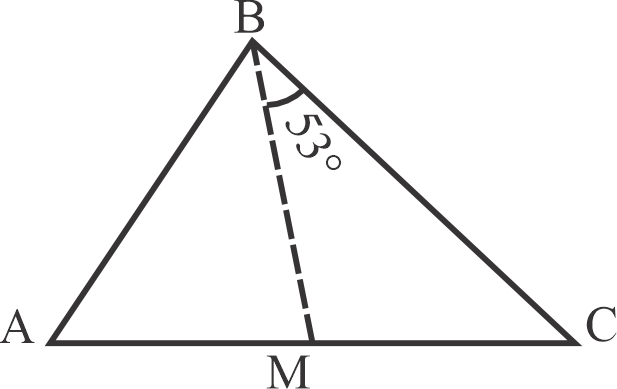
\includegraphics[width=4.4cm]{imagenes/CEPRE-UNA2024-I/etapa2/bio/geo1c24-I.png}
	\end{center}
	\begin{enumerate}[label=\alph*)]
		\item 30 cm
		\item 45 cm
		\item 50 cm
		\item 40 cm
		\item 35 cm
	\end{enumerate}
	\textbf{Respuesta correcta:} a)
	
	\vspace{2mm}
	\textbf{Solucionario:}
	
	\begin{center}
		\begin{minipage}{0.45\textwidth}
			
		Piden $BM=x$
		
		Trazamos $MN$ base media del triángulo ABC.

		Como $N$ es punto medio  de $BC$ y $HC=2MN$, se tiene que $MN$ también es base media del triángulo rectángulo $BHC$.
		
		Entonces, el triángulo $BHC$ es notable de $37^\circ$ y $53^\circ$, por lo que sus lados están en razón:
		
		$3k,\ 4k,\ 5k$
		
		Del gráfico se obtiene:
		
		$2x=60$
		
		Por tanto:
		
		$x=30\text{ cm}$
		
		\fbox{$30\text{ cm}$}
			\vspace{6mm}
		\end{minipage}
		\hfill
		\begin{minipage}{0.45\textwidth}
			\centering
			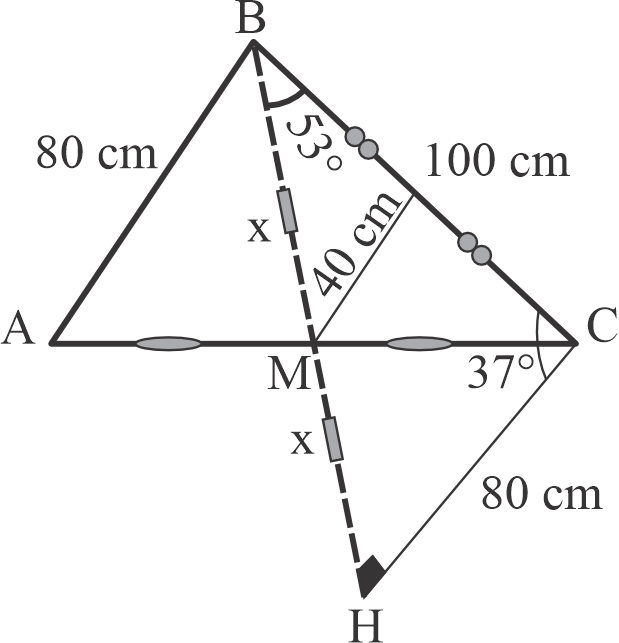
\includegraphics[width=4cm]{imagenes/CEPRE-UNA2024-I/etapa2/bio/geo1c24-Ir.png}
		\end{minipage}
		\end{center}
	
	\vspace{6mm}
	
	\item Se tiene un hexágono equiángulo $ABCDEF$ de tal manera que $AB=3$, $BC=6$, $EF=2$ y $AF=9$. Calcule las longitudes de $\overline{CD}$ y $\overline{DE}$.
	\begin{enumerate}[label=\alph*)]
		\item 4 y 7
		\item 5 y 7
		\item 7 y 6
		\item 7 y 3
		\item 4 y 5
	\end{enumerate}
	\textbf{Respuesta correcta:} b)
	
	\vspace{2mm}
	\textbf{Solucionario:}\\[1mm]
	
	
		\begin{center}
		\begin{minipage}{0.45\textwidth}
			
	
			Como el polígono es equiángulo, cada ángulo exterior mide:
			
			$\dfrac{360^\circ}{6}=60^\circ$
			
			Al prolongar los lados, se forman triángulos equiláteros auxiliares.
			
			De la figura se obtiene que:
			
			$PR=14$
			\qquad y \qquad
			$PQ=14$
			
			Entonces:
			
			$3+6+x=14$
			
			$9+x=14$
			
			$x=5$
			
			Además:
			
			$x+y+2=14$
			
			$5+y+2=14$
			
			$y=7$
			
			Por lo tanto:
			
			$CD=x=5,\qquad DE=y=7$
			
			\fbox{$CD=5,\ DE=7$}
			\vspace{6mm}
		\end{minipage}
		\hfill
		\begin{minipage}{0.45\textwidth}
			\centering
			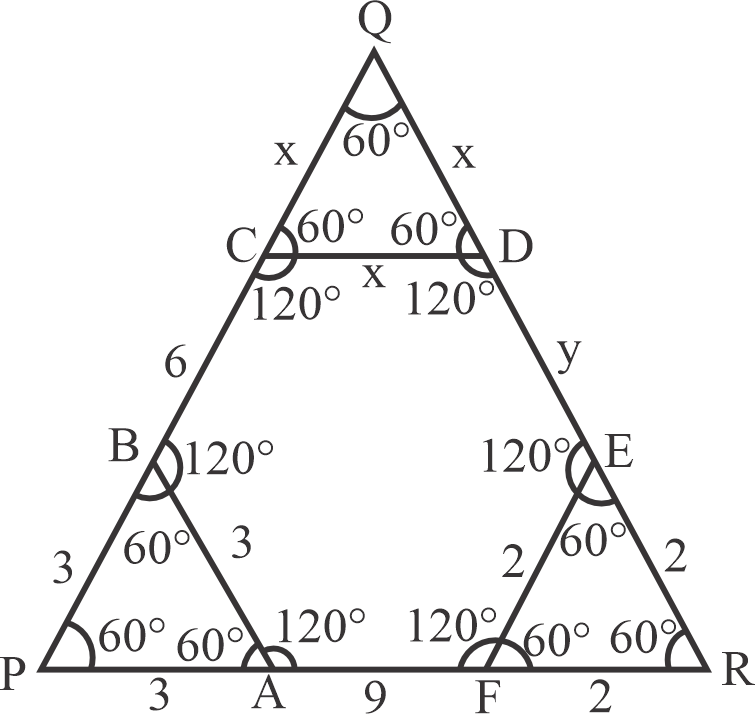
\includegraphics[width=4.2cm]{imagenes/CEPRE-UNA2024-I/etapa2/bio/geo2c24-Ir.png}
		\end{minipage}
	\end{center}
	

	
	\vspace{6mm}
	
	\item Marcos construye una mesa cuyo tablero tiene la forma de un trapecio isósceles, tal como se muestra en el gráfico. Calcule el perímetro del tablero de la mesa.
	\begin{center}
		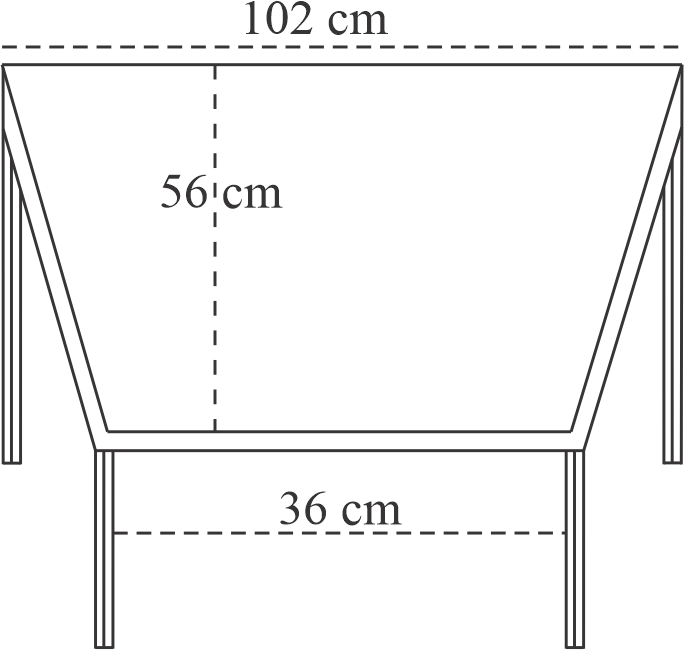
\includegraphics[width=4.3cm]{imagenes/CEPRE-UNA2024-I/etapa2/bio/geo3c24-I.png}
	\end{center}
	
	\begin{enumerate}[label=\alph*)]
		\item 230 cm
		\item 258 cm
		\item 260 cm
		\item 268 cm
		\item 278 cm
	\end{enumerate}
	\textbf{Respuesta correcta:} d)
	
	\vspace{2mm}
	\textbf{Solucionario:}

			\begin{center}
		\begin{minipage}{0.45\textwidth}
			
			
		Bases:

		$B=102,\qquad b=36,\qquad h=56$
		
		La semidiferencia de bases es:\\
		
		$\dfrac{102-36}{2}=33$\\
		
		Cada lado oblicuo mide:\\
		
		$l=\sqrt{33^2+56^2}=\sqrt{1089+3136}=\sqrt{4225}=65$
		
		Entonces el perímetro es:
		
		$P=102+36+65+65=$\fbox{$268$}
			\vspace{6mm}
		\end{minipage}
		\hfill
		\begin{minipage}{0.45\textwidth}
			\centering
			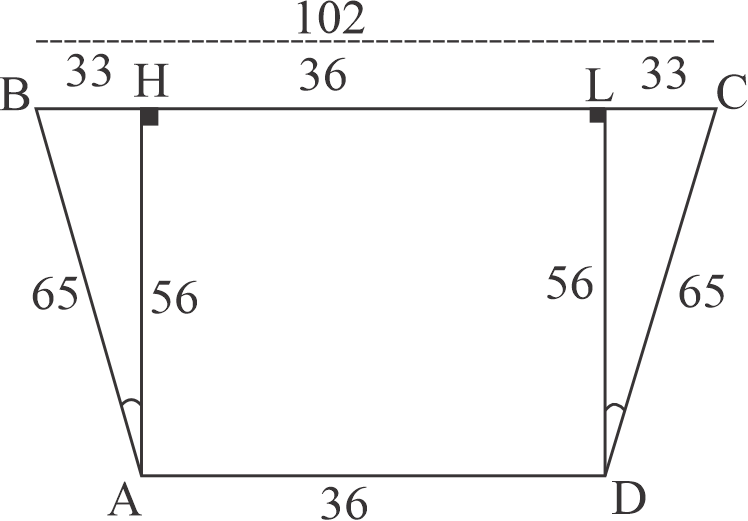
\includegraphics[width=4.5cm]{imagenes/CEPRE-UNA2024-I/etapa2/bio/geo3c24-Ir.png}
		\end{minipage}
	\end{center}
	
	\vspace{6mm}
	
\end{enumerate}

\subsection*{Trigonometría}

\begin{enumerate}[resume]

	
	\item En la figura, calcule el área de la región sombreada si $OA=OB$ y $AC=BD$.
	
	\begin{center}
		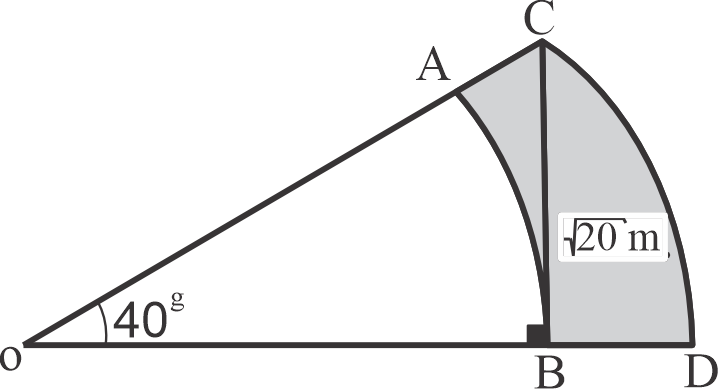
\includegraphics[width=4.3cm]{imagenes/CEPRE-UNA2024-I/etapa2/bio/trigo1c24-I.png}
	\end{center}
	
	\begin{enumerate}[label=\alph*)]
		\item $\pi\ m^2$
		\item $2\pi\ m^2$
		\item $3\pi\ m^2$
		\item $4\pi\ m^2$
		\item $5\pi\ m^2$
	\end{enumerate}
	\textbf{Respuesta correcta:} b)
	
	\vspace{2mm}
	\textbf{Solucionario:}\\[1mm]
	Como $40^g=\dfrac{40\pi}{200}=\dfrac{\pi}{5}\text{ rad}$
	
	$\theta=\dfrac{\pi}{5}$
	
	Además, en el triángulo rectángulo formado por los radios y la distancia entre circunferencias:
	
	$R^2=r^2+(\sqrt{20})^2$
	
	$R^2-r^2=20$
	
	El área sombreada es la diferencia de dos sectores:
	
	$A_{\text{sombreada}}=\dfrac{\theta R^2}{2}-\dfrac{\theta r^2}{2}$
	
	$=\dfrac{\theta}{2}(R^2-r^2)$
	
	$=\dfrac{1}{2}\cdot \dfrac{\pi}{5}\cdot 20$
	
	$=2\pi \text{ m}^2$
	
	\fbox{$2\pi \text{ m}^2$}
	
	
	\vspace{6mm}
	
	\item En la figura, si $AB=12\sqrt{3}$ y $BC=4\sqrt{3}$, calcule $AD+CD$.
	
	\begin{center}
		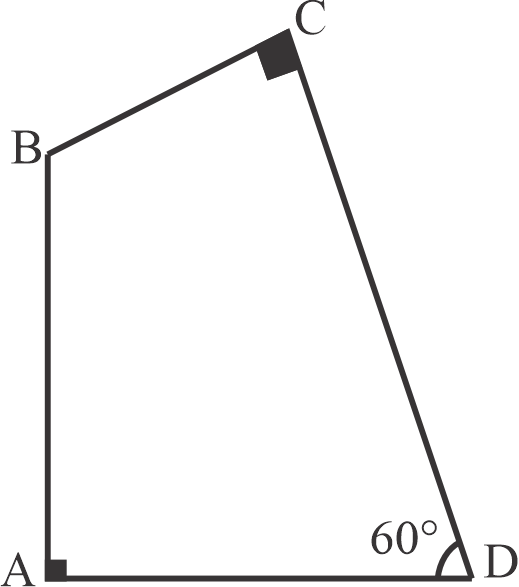
\includegraphics[width=3.8cm]{imagenes/CEPRE-UNA2024-I/etapa2/bio/trigo2c24-I.png}
	\end{center}
	
	\begin{enumerate}[label=\alph*)]
		\item 40
		\item 46
		\item 38
		\item 50
		\item 48
	\end{enumerate}
	\textbf{Respuesta correcta:} e)
	
	\vspace{2mm}
	\textbf{Solucionario:}

	En el gráfico inicial se continua con el trazo de $AB$ y $DC$ hacia el punto $A$, se reconoce que los triángulos $ADE$ y $BCE$ son triángulos notables de $30^\circ$ y $60^\circ$.
	
	Por ello, los segmentos correspondientes resultan:
	
	$AD=20$
	\qquad y \qquad
	$DC=28$
	
	Entonces:
	
	$AD+DC=20+28=$\fbox{$48$}
	
	\vspace{6mm}
	

	\item Si $3\sen x+4\cos x=5$, calcule $\tan x+\dfrac{5}{4}$.
	\begin{enumerate}[label=\alph*)]
		\item 1
		\item 0
		\item 2
		\item $\dfrac{1}{4}$
		\item $\dfrac{3}{4}$
	\end{enumerate}
	\textbf{Respuesta correcta:} c)
	
	\vspace{2mm}
	\textbf{Solucionario:}\\[1mm]
	
	\begin{center}
		\begin{tikzpicture}[scale=0.9]
			\draw[very thick] (0,0) -- (4,0) -- (4,3) -- cycle;
			\draw[very thick] (3.7,0) -- (3.7,0.3) -- (4,0.3);
			\node at (2, -0.35) {$4$};
			\node at (4.35,1.5) {$3$};
			\node at (1.7,1.8) {$5$};
			\draw[very thick] (0.8,0) arc[start angle=0,end angle=37,radius=0.8];
			\node at (1.15,0.35) {$37^\circ$};
			\draw[very thick] (4,2.2) arc[start angle=270,end angle=215,radius=0.8];
			\node at (3.55,2) {$53^\circ$};
		\end{tikzpicture}
	\end{center}
	
	Dividimos entre $5$:
	
	$\dfrac{3}{5}\sen x+\dfrac{4}{5}\cos x=1$
	
	Como $\dfrac{3}{5}$ y $\dfrac{4}{5}$ corresponden a un triángulo notable $3$-$4$-$5$, tomamos:
	
	$\cos 53^\circ=\dfrac{3}{5}, \qquad \sen 53^\circ=\dfrac{4}{5}$
	
	Entonces:
	
	$\cos 53^\circ \sen x+\sen 53^\circ \cos x=1$
	
	
	$\sen(x+53^\circ)=1$
	
	
	$x+53^\circ=90^\circ$
	
	$x=37^\circ$
	
	
	$\tan x+\dfrac{5}{4}=\tan 37^\circ+\dfrac{5}{4}$
	
	$=\dfrac{3}{4}+\dfrac{5}{4}=$\fbox{$2$}
	
	\vspace{6mm}
	
\end{enumerate}

\subsection*{Física}

\begin{enumerate}[resume]
	
	
	\item En la figura, calcule el valor de la fuerza $\vec{F}$ para que el cuerpo de 40 N de peso permanezca en equilibrio.
	
	\begin{center}
		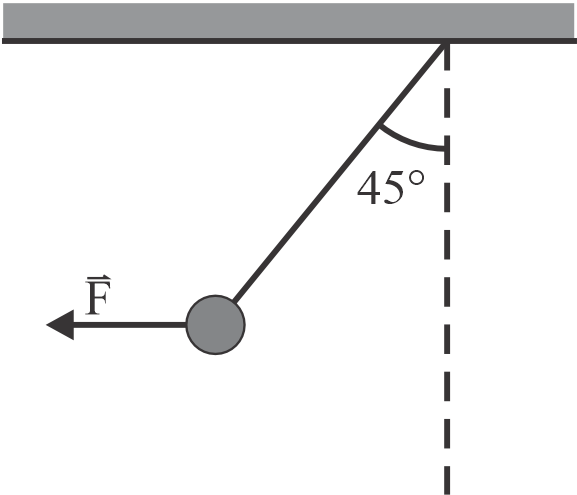
\includegraphics[width=4cm]{imagenes/CEPRE-UNA2024-I/etapa2/bio/fisica1c24-I.png}
	\end{center}
	
	\begin{enumerate}[label=\alph*)]
		\item 20 N
		\item $20\sqrt{2}$ N
		\item 40 N
		\item $40\sqrt{2}$ N
		\item 45 N
	\end{enumerate}
	\textbf{Respuesta correcta:} c)
	
	\vspace{2mm}
	\textbf{Solucionario:}\\[1mm]
	La tensión forma $45^\circ$ con la vertical. En equilibrio:
	
	$T\cos45^\circ=40$
	
	$T=\dfrac{40}{\cos45^\circ}=40\sqrt2$
	
	La fuerza horizontal es:
	
	$F=T\sen45^\circ=40\sqrt2\cdot \dfrac{\sqrt2}{2}=$\fbox{$40N$}
	
	\vspace{6mm}
	

	
	\item Desde la superficie terrestre se lanza un proyectil con una velocidad de 50 m/s formando un ángulo de $53^\circ$ con la horizontal. Determine el valor de la velocidad del proyectil en el punto más alto de su trayectoria.
	\begin{enumerate}[label=\alph*)]
		\item 20 m/s
		\item 30 m/s
		\item 40 m/s
		\item 50 m/s
		\item 60 m/s
	\end{enumerate}
	\textbf{Respuesta correcta:} b)
	
	\vspace{2mm}
	\textbf{Solucionario:}\\[1mm]
	En el punto más alto, la componente vertical es cero y solo queda la horizontal:
	
	$v_x=50\cos53^\circ$
	
	Usando:
	
	$\cos53^\circ=\dfrac35$
	
	se obtiene:
	
	$v_x=50\cdot \dfrac{3}{5}=$\fbox{$30N$}
	
	\vspace{6mm}
	
	
	\item Una máquina soldadora de 1000 W funciona a un voltaje de 220 V. Determine la energía eléctrica que consume en 20 minutos de funcionamiento.
	\begin{enumerate}[label=\alph*)]
		\item 0,6 MJ
		\item 1,0 MJ
		\item 1,2 MJ
		\item 2,2 MJ
		\item 4,4 MJ
	\end{enumerate}
	\textbf{Respuesta correcta:} c)
	
	\vspace{2mm}
	\textbf{Solucionario:}\\[1mm]
	La energía es:
	
	$E=Pt$
	
	Con:
	
	$P=1000\text{ W},\qquad t=20\text{ min}=1200\text{ s}$
	
	Entonces:
	
	$E=1000(1200)=1\,200\,000\text{ J}=$\fbox{$1.2\text{ MJ}$}
	
	\vspace{6mm}
	
\end{enumerate}

  \subsection*{Química}

\begin{enumerate}[resume]
	
	\item Se tiene dos isótopos los cuales tienen 20 y 24 neutrones respectivamente. Si la suma de sus números de nucleones fundamentales es 104, determine la ubicación de dicho elemento en la tabla periódica.
	\begin{enumerate}[label=\alph*)]
		\item período 3: grupo 4B
		\item período 4: grupo 2B
		\item período 4: grupo 6B
		\item período 4: grupo 3B
		\item período 5: grupo 1B
	\end{enumerate}
	\textbf{Respuesta correcta:} b)
	
	\vspace{2mm}
	\textbf{Solucionario:}\\[1mm]
	Sea $Z$ el número atómico. Los números másicos son:
	
	$A_1=Z+20,\qquad A_2=Z+24$
	
	Su suma es 104:
	
	$(Z+20)+(Z+24)=104$
	
	$2Z+44=104$
	
	$2Z=60 \Rightarrow Z=30$
	
	El elemento con $Z=30$ es Zn, ubicado en período 4, grupo 2B.
	
	\vspace{6mm}
	
	\item Después del balanceo en medio ácido de la ecuación iónica:
	
	$\mathrm{Fe^{2+}_{(ac)}+ClO_3^-{}_{(ac)}\rightarrow Fe^{3+}_{(ac)}+Cl^-{}_{(ac)}}$
	
	indique el coeficiente del agua.
	\begin{enumerate}[label=\alph*)]
		\item 2
		\item 3
		\item 4
		\item 5
		\item 6
	\end{enumerate}
	\textbf{Respuesta correcta:} b)
	
	\vspace{2mm}
	\textbf{Solucionario:}\\[1mm]
	Semirreacciones:
	
	$Fe^{2+}\rightarrow Fe^{3+}+e^-$
	
	$ClO_3^-+6H^++6e^-\rightarrow Cl^-+3H_2O$
	
	Multiplicando la primera por 6 y sumando:
	
	$6Fe^{2+}+ClO_3^-+6H^+\rightarrow 6Fe^{3+}+Cl^-+3H_2O$
	
	El coeficiente del agua es \fbox{3}
	
	\vspace{6mm}
	
	\item Un balón contiene metano ($CH_4$) a $30^\circ C$ y 0,4 atm. Calcule la presión que tendrá si aumentamos la temperatura hasta $200^\circ C$ permaneciendo su volumen constante.
	\begin{enumerate}[label=\alph*)]
		\item 0,26 atm
		\item 0,29 atm
		\item 0,31 atm
		\item 0,38 atm
		\item 0,62 atm
	\end{enumerate}
	\textbf{Respuesta correcta:} e)
	
	\vspace{2mm}
	\textbf{Solucionario:}\\[1mm]
	A volumen constante:
	
	$\dfrac{P_1}{T_1}=\dfrac{P_2}{T_2}$
	
	Temperaturas absolutas:
	
	$T_1=30+273=303,\qquad T_2=200+273=473$
	
	Entonces:
	
	$P_2=0.4\cdot \dfrac{473}{303}\approx \fbox{0.62}$
	
	\vspace{6mm}
	
	\item Proporcione el nombre IUPAC del alcano cuya notación topológica es:
	
	\begin{center}
		
\includegraphics[width=4.5cm]{imagenes/CEPRE-UNA2024-I/etapa2/bio/quimica4c24-I.png}
	\end{center}
	
	\begin{enumerate}[label=\alph*)]
		\item 7-isobutil-2,3,6-trimetilundecano
		\item 5-isobutil-6,9,19-trimetilundecano
		\item 3-sec-butil-5,3,4-dimetilundecano
		\item 5-etil-5,6,11-trimetil-4-terbutilnonano
		\item 7-butil-2,3,6,9-tetrametildecano
	\end{enumerate}
	\textbf{Respuesta correcta:} a)
	
	\vspace{2mm}
	\textbf{Solucionario:}\\[1mm]
	Se identifica como cadena principal una de 11 carbonos, es decir, un undecano. Al numerar para obtener el menor conjunto de localizadores, se observan tres metilos en 2, 3 y 6, y un isobutil en 7. Por ello, el nombre correcto es:
	
	$\text{7-isobutil-2,3,6-trimetilundecano}$
	
	\vspace{6mm}
	
	\item El grupo de vitaminas B es muy complejo. Tenemos por ejemplo la vitamina $B_1$ cuya fórmula es $C_{12}H_{17}N_4OS$ y la vitamina $B_2$ cuya fórmula es $C_{17}H_{20}N_4O_6$. Entonces la suma de sus pesos moleculares es:
	\begin{enumerate}[label=\alph*)]
		\item 700
		\item 641
		\item 376
		\item 265
		\item 670
	\end{enumerate}
	\textbf{Respuesta correcta:} b)
	
	\vspace{2mm}
	\textbf{Solucionario:}\\[1mm]
	Usando masas atómicas: $C=12$, $H=1$, $N=14$, $O=16$, $S=32$.
	
	Para $B_1$:
	
	$12(12)+17(1)+4(14)+16+32=265$
	
	Para $B_2$:
	
	$17(12)+20(1)+4(14)+6(16)=376$
	
	Suma:
	
	\fbox{$265+376=641$}
	
	\vspace{6mm}
	
\end{enumerate}

\subsection*{Biología y Anatomía}

\begin{enumerate}[resume]
	
	\item Juan desarrolla anemia si su cuerpo no produce suficientes glóbulos rojos. ¿Cuál es el bioelemento insuficiente que presenta?
	\begin{enumerate}[label=\alph*)]
		\item Insulina
		\item Hierro
		\item Glucagón
		\item Iodo
		\item Glucosa
	\end{enumerate}
	\textbf{Respuesta correcta:} b)
	
	\vspace{2mm}
	\textbf{Solucionario:}\\[1mm]
	La anemia suele asociarse a la deficiencia de hierro, porque este elemento es esencial para la formación de hemoglobina y glóbulos rojos.
	
	\vspace{6mm}
	
	\item Los animales que pueden variar su temperatura corporal modificando su comportamiento en estrecha relación a la temperatura ambiental se denominan:
	\begin{enumerate}[label=\alph*)]
		\item homeotermos.
		\item poiquilotermos.
		\item endotermos.
		\item homotermos.
		\item depredadores.
	\end{enumerate}
	\textbf{Respuesta correcta:} b)
	
	\vspace{2mm}
	\textbf{Solucionario:}\\[1mm]
	Los poiquilotermos son organismos cuya temperatura corporal varía de acuerdo con la temperatura del ambiente.
	
	\vspace{6mm}
	
	\item Algunas serpientes incuban sus huevos en el interior del oviducto donde eclosionan liberando sus crías. Este tipo de nacimiento corresponde a:
	\begin{enumerate}[label=\alph*)]
		\item ovíparos.
		\item ovovivíparos.
		\item metamorfosis.
		\item vivíparos.
		\item fragmentación.
	\end{enumerate}
	\textbf{Respuesta correcta:} b)
	
	\vspace{2mm}
	\textbf{Solucionario:}\\[1mm]
	En los ovovivíparos, los huevos permanecen dentro del cuerpo de la madre hasta su eclosión, pero el embrión se nutre del huevo, no directamente de la madre.
	
	\vspace{6mm}
	
	\item Las haustras, tenias musculares y apéndices cecales son estructuras que corresponden al:
	\begin{enumerate}[label=\alph*)]
		\item estómago.
		\item intestino delgado.
		\item esófago.
		\item hígado.
		\item intestino grueso.
	\end{enumerate}
	\textbf{Respuesta correcta:} e)
	
	\vspace{2mm}
	\textbf{Solucionario:}\\[1mm]
	Las haustras, tenias del colon y apéndices epiploicos son características anatómicas del intestino grueso.
	
	\vspace{6mm}
	
	\item En el ciclo del nitrógeno, intervienen bacterias nitrificantes y bacterias fijadoras de nitrógeno. Ejemplos de ellas son:
	\begin{enumerate}[label=\alph*)]
		\item nitrosomonas -- rhizobium.
		\item nitrosomonas -- nitrobacter.
		\item rhizobium -- azotobacter.
		\item nitrobacter -- nitrosomonas.
		\item azotobacter -- rhizobium.
	\end{enumerate}
	\textbf{Respuesta correcta:} a)
	
	\vspace{2mm}
	\textbf{Solucionario:}\\[1mm]
	\textit{Nitrosomonas} es bacteria nitrificante y \textit{Rhizobium} es fijadora de nitrógeno. La pareja correcta es:
	
	$\text{nitrosomonas -- rhizobium}$
	
	\vspace{6mm}
	
	\item El principal efecto de los compuestos fluorocarbonados utilizados como refrigerantes es que al ser liberados a la atmósfera:
	\begin{enumerate}[label=\alph*)]
		\item producen acumulación en tejidos orgánicos.
		\item provocan efecto smog fotoquímico.
		\item provocan la lluvia ácida.
		\item destruyen la capa de ozono.
		\item producen la eutroficación.
	\end{enumerate}
	\textbf{Respuesta correcta:} d)
	
	\vspace{2mm}
	\textbf{Solucionario:}\\[1mm]
	Los clorofluorocarbonos y compuestos similares afectan la capa de ozono estratosférica, favoreciendo su destrucción.
	
	\vspace{6mm}
	
\end{enumerate}

\subsection*{Psicología y Filosofía}

\begin{enumerate}[resume]
	
	\item El principio y el fin de todo conocimiento es la:
	\begin{enumerate}[label=\alph*)]
		\item teoría.
		\item especulación.
		\item ciencia.
		\item práctica.
		\item argumentación.
	\end{enumerate}
	\textbf{Respuesta correcta:} d)
	
	\vspace{2mm}
	\textbf{Solucionario:}\\[1mm]
	En filosofía se sostiene que la práctica es la base y comprobación del conocimiento, por lo que se considera el principio y fin del mismo.
	
	\vspace{6mm}
	
	\item Cuando la persona moral se da cuenta que los actos que realiza son buenos o malos, estamos haciendo referencia a:
	\begin{enumerate}[label=\alph*)]
		\item libertad moral.
		\item acto moral.
		\item conciencia moral.
		\item responsabilidad moral.
		\item libertad de conciencia.
	\end{enumerate}
	\textbf{Respuesta correcta:} c)
	
	\vspace{2mm}
	\textbf{Solucionario:}\\[1mm]
	La conciencia moral es la capacidad de juzgar los propios actos como buenos o malos.
	
	\vspace{6mm}
	
	\item La disciplina filosófica que se encarga de estudiar la ciencia y la estructura del conocimiento es la:
	\begin{enumerate}[label=\alph*)]
		\item axiología.
		\item epistemología.
		\item traumatología.
		\item sociología.
		\item fenomenología.
	\end{enumerate}
	\textbf{Respuesta correcta:} b)
	
	\vspace{2mm}
	\textbf{Solucionario:}\\[1mm]
	La epistemología estudia la naturaleza, origen y validez del conocimiento científico.
	
	\vspace{6mm}
	
	\item Es el cambio más complejo que incluye transformaciones en el funcionamiento y desarrollo de la inteligencia, creatividad, sociabilidad y moralidad.
	\begin{enumerate}[label=\alph*)]
		\item Cambio cualitativo
		\item Cambio cuantitativo
		\item Metamorfosis
		\item Cambio dimensional
		\item Maduración
	\end{enumerate}
	\textbf{Respuesta correcta:} a)
	
	\vspace{2mm}
	\textbf{Solucionario:}\\[1mm]
	El cambio cualitativo implica modificaciones profundas en la manera de pensar, actuar y desarrollarse, no solo aumento en cantidad. Por ello se relaciona con inteligencia, creatividad, sociabilidad y moralidad.
	
	\vspace{6mm}
	
\end{enumerate}

\subsection*{Geografía}

\begin{enumerate}[resume]
	
	\item La unidad minera que explota yacimientos de cobre en el departamento de Apurímac es:
	\begin{enumerate}[label=\alph*)]
		\item Antamina.
		\item Las Bambas.
		\item Cobriza.
		\item Tintaya.
		\item Cerro Verde.
	\end{enumerate}
	\textbf{Respuesta correcta:} b)
	
	\vspace{2mm}
	\textbf{Solucionario:}\\[1mm]
	Las Bambas es el importante proyecto cuprífero ubicado en la región Apurímac.
	
	\vspace{6mm}
	
	\item El mar peruano es considerado uno de los más ricos y variados a nivel mundial debido a la:
	\begin{enumerate}[label=\alph*)]
		\item ubicación geográfica del Perú.
		\item cercanía de la Cordillera de los Andes.
		\item presencia de nubes stratos.
		\item descarga constante de sedimentos de ríos.
		\item abundancia de fitoplancton.
	\end{enumerate}
	\textbf{Respuesta correcta:} e)
	
	\vspace{2mm}
	\textbf{Solucionario:}\\[1mm]
	La riqueza del mar peruano se debe, entre otros factores, a la abundancia de fitoplancton, base de la cadena alimenticia marina.
	
	\vspace{6mm}
	
\end{enumerate}

\subsection*{Historia}

\begin{enumerate}[resume]
	
	\item Fue el impuesto que gravaba los cargos públicos, lo que debían pagar aquellos que asumían un cargo administrativo antes de ejercer el mismo.
	\begin{enumerate}[label=\alph*)]
		\item Derecho de avería
		\item El almojarifazgo
		\item El tributo indígena
		\item La alcabala
		\item La media anata
	\end{enumerate}
	\textbf{Respuesta correcta:} e)
	
	\vspace{2mm}
	\textbf{Solucionario:}\\[1mm]
	La media anata era el tributo que debían pagar quienes accedían a determinados cargos públicos.
	
	\vspace{6mm}
	
	\item Es el presidente que, en 1933, pasaba revista a los 30 mil movilizables en el antiguo Hipódromo de Santa Beatriz, hoy Campo de Marte en Lima, y fue asesinado por Abelardo Mendoza Leyva de tres tiros de revólver.
	\begin{enumerate}[label=\alph*)]
		\item Oscar Raymundo Benavides
		\item Manuel Prado Ugarteche
		\item José Luis Bustamante y Rivero
		\item Luís Miguel Sánchez Cerro
		\item Augusto Bernardino Leguía
	\end{enumerate}
	\textbf{Respuesta correcta:} d)
	
	\vspace{2mm}
	\textbf{Solucionario:}\\[1mm]
	El presidente asesinado en 1933 fue Luis Miguel Sánchez Cerro.
	
	\vspace{6mm}
	
\end{enumerate}

\subsection*{Educación Cívica}

\begin{enumerate}[resume]
	
	\item Marcos está casado con Juana por un período de 5 años; sin embargo, Juana toma conocimiento que Marcos tiene un hijo extramatrimonial de 1 año, hecho que corrobora con el acta de nacimiento. ¿Qué causal podría invocar Juana para que declaren fundada su demanda de divorcio?
	\begin{enumerate}[label=\alph*)]
		\item Servicia
		\item Hijo extramatrimonial
		\item Engaño
		\item Adulterio
		\item Infidelidad
	\end{enumerate}
	\textbf{Respuesta correcta:} d)
	
	\vspace{2mm}
	\textbf{Solucionario:}\\[1mm]
	El hijo de 1 año prueba que Marcos tuvo relaciones con otra mujer durante el matrimonio, lo que constituye adulterio.
	
	\vspace{6mm}
	
	\item En el año 2019, entró en vigencia la ley de plásticos como respuesta del país ante la grave situación que enfrentan los mares del mundo por la contaminación. En el corto plazo, los supermercados fueron prohibidos de entregar bolsas de plástico no reutilizables, fabricar sorbetes para el consumo interno, entre otras medidas importantes. Todo lo anterior está vinculado con la preservación del medio ambiente sano que es clasificado como un derecho humano de:
	\begin{enumerate}[label=\alph*)]
		\item primera generación.
		\item segunda generación.
		\item tercera generación.
		\item cuarta generación.
		\item pre generación.
	\end{enumerate}
	\textbf{Respuesta correcta:} c)
	
	\vspace{2mm}
	\textbf{Solucionario:}\\[1mm]
	Los derechos relacionados con el ambiente sano, la paz y el desarrollo pertenecen a la tercera generación de derechos humanos.
	
	\vspace{6mm}
	
\end{enumerate}

\subsection*{Economía}

\begin{enumerate}[resume]
	
	\item La estructura del presupuesto público en el Perú comprende los gastos corrientes que:
	\begin{enumerate}[label=\alph*)]
		\item incluye el pago de salarios del personal que labora en el sector público.
		\item son destinados a proyectos de inversión a largo plazo.
		\item son relacionados con la deuda externa del país.
		\item son categorías separadas en el presupuesto y no están vinculadas a actividades diarias.
		\item incluye los otros gastos de capital.
	\end{enumerate}
	\textbf{Respuesta correcta:} a)
	
	\vspace{2mm}
	\textbf{Solucionario:}\\[1mm]
	Los gastos corrientes financian el funcionamiento ordinario del Estado, como remuneraciones, bienes y servicios.
	
	\vspace{6mm}
	
	\item Es el proceso de acumulación progresiva durante un período más o menos prolongado de una parte de los ingresos percibidos.
	\begin{enumerate}[label=\alph*)]
		\item El ingreso
		\item La producción
		\item La inversión
		\item El capital
		\item El ahorro
	\end{enumerate}
	\textbf{Respuesta correcta:} e)
	
	\vspace{2mm}
	\textbf{Solucionario:}\\[1mm]
	El ahorro consiste en reservar o acumular una parte del ingreso para uso futuro.
	
	\vspace{6mm}
	
\end{enumerate}

\subsection*{Comunicación}

\begin{enumerate}[resume]
	
	\item En una conversación, un botánico afirma: “Las plantas del patio crecen al recibir luz solar y agua. Las plantas del vecino crecen al recibir luz solar y agua. Las plantas del jardín botánico crecen al recibir luz solar y agua. Entonces las plantas crecen al recibir la luz solar y el agua”.
	
	Considerando la redacción, las ideas están expresadas en forma:
	\begin{enumerate}[label=\alph*)]
		\item deductiva.
		\item inductiva.
		\item mixta.
		\item paremiológica.
		\item compleja.
	\end{enumerate}
	\textbf{Respuesta correcta:} b)
	
	\vspace{2mm}
	\textbf{Solucionario:}\\[1mm]
	Se presentan varios casos particulares y luego una conclusión general. Eso corresponde a razonamiento inductivo.
	
	\vspace{6mm}
	
	\item Cuando la Constitución Política del Perú declara como idiomas oficiales al quechua, aimara y lenguas originarias amazónicas quiere decir que:
	\begin{enumerate}[label=\alph*)]
		\item no se deben usar en público.
		\item se obliga su uso a todos los ciudadanos.
		\item están facultados para uso público e institucional.
		\item se reconocen como un derecho humano.
		\item solo pueden ser usados por los nativos.
	\end{enumerate}
	\textbf{Respuesta correcta:} c)
	
	\vspace{2mm}
	\textbf{Solucionario:}\\[1mm]
	Ser idioma oficial significa que puede usarse legítimamente en ámbitos públicos e institucionales, dentro de su zona de predominio.
	
	\vspace{6mm}
	
	\item Cuando un narrador exagera las cualidades físicas o morales de un personaje, genera una descripción denominada:
	\begin{enumerate}[label=\alph*)]
		\item etopeya.
		\item retrato.
		\item prosopografía.
		\item topografía.
		\item caricatura.
	\end{enumerate}
	\textbf{Respuesta correcta:} e)
	
	\vspace{2mm}
	\textbf{Solucionario:}\\[1mm]
	La caricatura exagera rasgos físicos o morales. La etopeya describe rasgos morales, la prosopografía físicos, y la topografía lugares.
	
	\vspace{6mm}
	
	\item Complete el enunciado.
	
	El desarrollo social se refleja en el signo lingüístico gracias a la \rule{2cm}{0.15mm} y el caos lingüístico se evita gracias a la \rule{2cm}{0.15mm}
	\begin{enumerate}[label=\alph*)]
		\item sincronía -- diacronía.
		\item arbitrariedad -- linealidad.
		\item mutabilidad -- inmutabilidad.
		\item diacronía -- sincronía.
		\item linealidad -- arbitrariedad.
	\end{enumerate}
	\textbf{Respuesta correcta:} c)
	
	\vspace{2mm}
	\textbf{Solucionario:}\\[1mm]
	El signo lingüístico es mutable porque cambia socialmente, e inmutable porque no puede alterarse arbitrariamente por un individuo.
	
	\vspace{6mm}
	
\end{enumerate}

\subsection*{Literatura}

\begin{enumerate}[resume]
	
	\item El tema central del cuento \textit{Funes, el memorioso} de Borges es la:
	\begin{enumerate}[label=\alph*)]
		\item influencia de la literatura clásica en la mentalidad de Funes.
		\item representación de la vida cotidiana en un arrabal sudamericano.
		\item dualidad entre el pasado y el presente en la vida de Ireneo Funes.
		\item alineación en un mundo donde nadie comprende.
		\item paradoja de la memoria perfecta.
	\end{enumerate}
	\textbf{Respuesta correcta:} e)
	
	\vspace{2mm}
	\textbf{Solucionario:}\\[1mm]
	El cuento muestra cómo una memoria absoluta, lejos de ser una ventaja total, se vuelve una limitación. Por eso el tema es la paradoja de la memoria perfecta.
	
	\vspace{6mm}
	
	\item En una obra de Clorinda Matto de Turner, dos enamorados de origen indígena, Manuel y Margarita, se ven impedidos de concretar su amor al descubrir que son hermanos. ¿A qué novela nos estamos refiriendo?
	\begin{enumerate}[label=\alph*)]
		\item Índole
		\item Herencia
		\item Aves sin Nido
		\item Tradiciones Cuzqueñas y Leyendas
		\item Ima Súmac
	\end{enumerate}
	\textbf{Respuesta correcta:} c)
	
	\vspace{2mm}
	\textbf{Solucionario:}\\[1mm]
	Esa trama corresponde a \textit{Aves sin Nido}, novela de denuncia social de Clorinda Matto de Turner.
	
	\vspace{6mm}
	
\end{enumerate}

\subsection*{Razonamiento Matemático}

\begin{enumerate}[resume]
	
	\item Según el gráfico, G es baricentro del $\triangle ABC$. Si el área de la región triangular $ABC$ es $180\,u^2$, calcule el área de la región sombreada.
	
	\begin{center}
		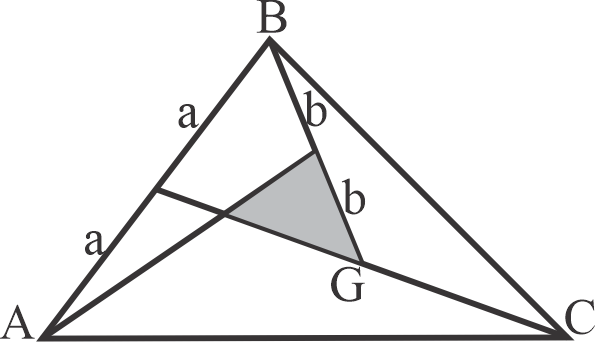
\includegraphics[width=4.5cm]{imagenes/CEPRE-UNA2024-I/etapa2/bio/rm1c24-I.png}
	\end{center}
	
	\begin{enumerate}[label=\alph*)]
		\item $20\,u^2$
		\item $10\,u^2$
		\item $15\,u^2$
		\item $25\,u^2$
		\item $18\,u^2$
	\end{enumerate}
	\textbf{Respuesta correcta:} a)
	
	\vspace{2mm}
	\textbf{Solucionario:}\\[1mm]
	Usando que $G$ es baricentro, las medianas dividen al triángulo en regiones con relaciones de área conocidas. La región sombreada resulta ser la doceava parte del área total:
	
	$\dfrac{180}{12}=15$
	
	Por tanto:
	
	$A_{\text{sombreada}}=$\fbox{$15u^2$}
	
	\vspace{6mm}
	
	\item Se define el operador
	
	$\boxed{\begin{matrix} b\\ a \end{matrix}}X^{n-1}=\dfrac{1}{n}(b^n-a^n)$\\
	
	Halle $m$ en\\
	
	$\boxed{\begin{matrix} 10\\ 1 \end{matrix}}X^2= \boxed{\begin{matrix} m\\ \sqrt{10} \end{matrix}}X$
	
	\begin{enumerate}[label=\alph*)]
		\item 14
		\item 18
		\item 20
		\item 22
		\item 26
	\end{enumerate}
	\textbf{Respuesta correcta:} e)
	
	\vspace{2mm}
	\textbf{Solucionario:}\\[1mm]
	En la izquierda, $n-1=2\Rightarrow n=3$:
	
	$\boxed{\begin{matrix} 10\\ 1 \end{matrix}}X^2=\dfrac13(10^3-1^3)=\dfrac{999}{3}=333$
	
	En la derecha, $n-1=1\Rightarrow n=2$:
	
	$\boxed{\begin{matrix} m\\ \sqrt{10} \end{matrix}}X=\dfrac12(m^2-10)$
	
	Igualando:
	
	$\dfrac12(m^2-10)=333$
	
	$m^2-10=666$
	
	$m^2=676 \Rightarrow m=$\fbox{$26$}
	
	\vspace{6mm}
	
	\item Al preguntarle por su edad a Silvia, ella contestó: “mi edad es la suma de todos aquellos números naturales tales que el cuadrado de su quíntuplo disminuido en 4 es mayor que 16 pero menor que 900”. ¿Cuál es la edad de Silvia?
	\begin{enumerate}[label=\alph*)]
		\item 20
		\item 19
		\item 17
		\item 16
		\item 18
	\end{enumerate}
	\textbf{Respuesta correcta:} a)
	
	\vspace{2mm}
	\textbf{Solucionario:}\\[1mm]
	Interpretamos:
	
	$(5n-4)^2>16 \quad \text{y}\quad (5n-4)^2<900$
	
	Entonces:
	
	$4<5n-4<30$
	
	$8<5n<34$
	
	$\dfrac85<n<\dfrac{34}{5}$
	
	Los naturales son:
	
	$n=2,3,4,5,6$
	
	Su suma es:
	
	$2+3+4+5+6=$\fbox{$20$}
	
	\vspace{6mm}
	
	\item Calcule el valor de:
	
	$\sqrt{\dfrac{605\times 595+25}{316\times 284+256}}$
	\begin{enumerate}[label=\alph*)]
		\item 7
		\item 6
		\item 2
		\item 3
		\item 1
	\end{enumerate}
	\textbf{Respuesta correcta:} c)
	
	\vspace{2mm}
	\textbf{Solucionario:}
	
	Usamos productos notables:
	
	$605\cdot 595+25=(600+5)(600-5)+25=600^2-25+25=600^2$
	
	$316\cdot 284+256=(300+16)(300-16)+16^2=300^2-256+256=300^2$
	
	Entonces:
	
	$\sqrt{\dfrac{600^2}{300^2}}=\sqrt{4}=$\fbox{$2$}
	
	\vspace{6mm}
	
	\item Halle $x-y$ si
	
	\begin{center}
		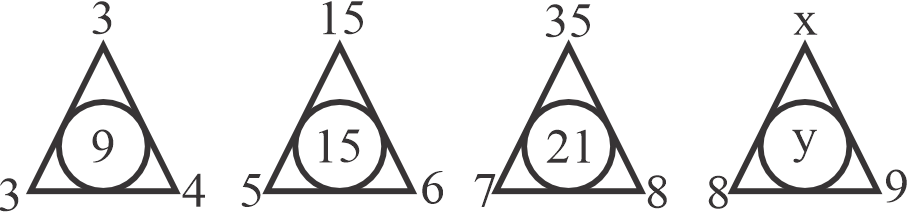
\includegraphics[width=7.8cm]{imagenes/CEPRE-UNA2024-I/etapa2/bio/rm5c24-I.png}
	\end{center}
	
	\begin{enumerate}[label=\alph*)]
		\item 38
		\item 28
		\item 46
		\item 54
		\item 63
	\end{enumerate}
	\textbf{Respuesta correcta:} a)
	
	\vspace{2mm}
	\textbf{Solucionario:}
	
	Primero calculamos el valor de $x$, siguiendo la secuencia de los números de la parte superior de cada triángulo:
	
	$2^2-1=3$
	
	$4^2-1=15$
	
	$6^2-1=35$
	
	Entonces:
	
	$8^2-1=64-1=63$
	
	Por lo tanto:
	
	$x=63$
	
	Ahora calculamos el valor de $y$ siguiendo la segunda secuencia:
	
	$(3\times 4)-3=9$
	
	$(5\times 6)-15=15$
	
	$(7\times 8)-35=21$
	
	Luego:
	
	$(8\times 9)-63=72-63=9$
	
	Así:
	
	$y=9$
	
	Finalmente:
	
	$x-y=63-9=$\fbox{$54$}
	
	\vspace{6mm}
	
	\item Determine la cantidad de círculos no sombreados en la posición 20:
	
	\begin{center}
		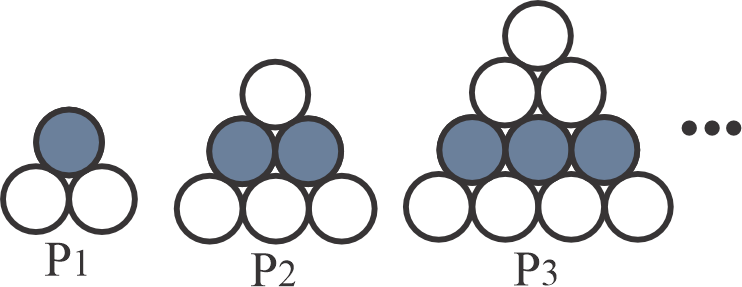
\includegraphics[width=4.5cm]{imagenes/CEPRE-UNA2024-I/etapa2/bio/rm6c24-I.png}
	\end{center}
	
	\begin{enumerate}[label=\alph*)]
		\item 211
		\item 210
		\item 201
		\item 190
		\item 189
	\end{enumerate}
	\textbf{Respuesta correcta:} a)
	
	\vspace{2mm}
	\textbf{Solucionario:}
	
	En la posición $n$, el total de círculos es:
	
	$T_{n+1}=\dfrac{(n+1)(n+2)}{2}$
	
	Los sombreados son $n$. Entonces los no sombreados son:
	
	$\dfrac{(n+1)(n+2)}{2}-n$
	
	Para $n=20$:
	
	$\dfrac{21\cdot 22}{2}-20=231-20=$\fbox{$211$}
	
	\vspace{6mm}
	
\end{enumerate}

\subsection*{Razonamiento Verbal}

\begin{enumerate}[resume]
	
	\item La raíz latina de CABALLO es:
	\begin{enumerate}[label=\alph*)]
		\item domus.
		\item equus.
		\item damnum.
		\item somnus.
		\item pectus.
	\end{enumerate}
	\textbf{Respuesta correcta:} b)
	
	\vspace{2mm}
	\textbf{Solucionario:}\\[1mm]
	La palabra latina para caballo es \textit{equus}.
	
	\vspace{6mm}
	
	\item Complete la oración:
	
	Las anomalías que \rule{2cm}{0.15mm} tu organismo son difíciles de comprender; por eso, \rule{2cm}{0.15mm} trataremos con médicos del extranjero.
	\begin{enumerate}[label=\alph*)]
		\item afectan - la
		\item tienen - las
		\item afecta - te
		\item presenta - las
		\item presentan - las
	\end{enumerate}
	\textbf{Respuesta correcta:} d)
	
	\vspace{2mm}
	\textbf{Solucionario:}\\[1mm]
	La forma correcta es:
	
	$\text{Las anomalías que presenta tu organismo...; por eso, las trataremos...}$
	
	En la primera parte, el verbo concuerda con “tu organismo”; en la segunda, el pronombre “las” reemplaza a “anomalías”.
	
	\vspace{6mm}
	
	\item ¿Qué término, por su generalidad, incluye a los otros?
	\begin{enumerate}[label=\alph*)]
		\item Cáncer
		\item Infección
		\item Afección
		\item Síndrome
		\item Cardiopatía
	\end{enumerate}
	\textbf{Respuesta correcta:} c)
	
	\vspace{2mm}
	\textbf{Solucionario:}\\[1mm]
	“Afección” es el término más general, porque puede incluir diversas enfermedades, trastornos o alteraciones.
	
	\vspace{6mm}
	
	\item Señale las afirmaciones correctas en los enunciados.
	
	I. Ómicrom es una enfermedad griega.\\
	II. Era es la diosa de la fertilidad.\\
	III. Iota es una letra griega.\\
	IV. La raíz griega andros significa niña.
	
	\begin{enumerate}[label=\alph*)]
		\item F V V F
		\item F F V V
		\item V F F V
		\item F V F V
		\item V V F F
	\end{enumerate}
	\textbf{Respuesta correcta:} a)
	
	\vspace{2mm}
	\textbf{Solucionario:}\\[1mm]
	I es falsa, porque ómicron es una letra griega.\\
	II se toma como verdadera en el planteamiento del examen.\\
	III es verdadera.\\
	IV es falsa, porque \textit{andros} significa hombre o varón.\\
	Por tanto:
	
	$F\ V\ V\ F$
	
	\vspace{6mm}
	
	\item El esquema general para ordenar las ideas es:
	
	I. Conclusión\\
	II. Tipos o clases\\
	III. Antecedentes\\
	IV. Características\\
	V. Definición
	
	\begin{enumerate}[label=\alph*)]
		\item V -- III -- II -- IV -- I
		\item III -- V -- IV -- II -- I
		\item I -- II -- III -- IV -- V
		\item IV -- III -- V -- II -- I
		\item V -- IV -- III -- II -- I
	\end{enumerate}
	\textbf{Respuesta correcta:} b)
	
	\vspace{2mm}
	\textbf{Solucionario:}\\[1mm]
	Un orden expositivo general razonable es: antecedentes, definición, características, tipos o clases y conclusión:
	
	$III - V - IV - II - I$
	
	\vspace{6mm}
	
	\item \textbf{COMPRENSIÓN DE TEXTO}
	
	“Si alguna vez adviertes que te miro a los ojos y una veta de amor reconoces en los míos, no pienses que deliro, piensa simplemente que puedes contar conmigo.
	
	Si otras veces me encuentras huraño sin motivo, no pienses que es flojera, igual puedes contar conmigo”.
	
	\hfill (Mario Benedetti)
	
	Es una conclusión sobre la destinataria del mensaje.
	\begin{enumerate}[label=\alph*)]
		\item Que no reconoce el amor.
		\item Que confunde flojera con amor.
		\item Que puede confundir el amor con el delirio.
		\item Que no piensa en su pareja.
		\item Que puede estar confundida.
	\end{enumerate}
	\textbf{Respuesta correcta:} c)
	
	\vspace{2mm}
	\textbf{Solucionario:}\\[1mm]
	El texto dice: “no pienses que deliro, piensa simplemente que puedes contar conmigo”. Esto indica que el autor anticipa que la destinataria podría interpretar su mirada de amor como un acto de delirio. Por lo tanto, la conclusión correcta es que ella puede confundir el amor con el delirio.
	
	\vspace{6mm}
	
\end{enumerate}

\subsection*{Inglés}

\begin{enumerate}[resume]
	
	\item Where is the toothbrush?
	
	\begin{center}
		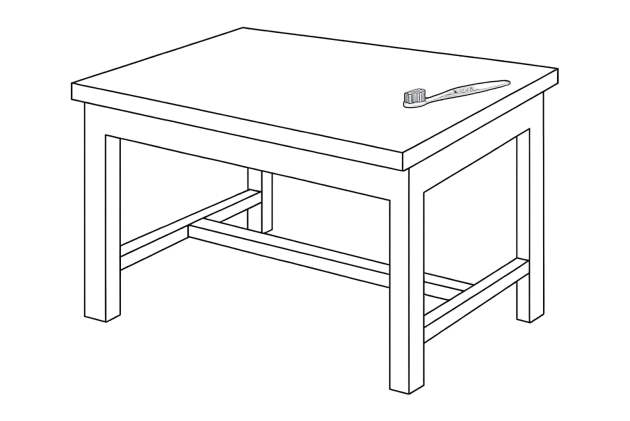
\includegraphics[width=4.5cm]{imagenes/CEPRE-UNA2024-I/etapa2/bio/ingles1c24-I.png}
	\end{center}
	
	\begin{enumerate}[label=\alph*)]
		\item It is near the table.
		\item It is in the table.
		\item It is under the table.
		\item It is next to the table.
		\item It is on the table.
	\end{enumerate}
	\textbf{Respuesta correcta:} e)
	
	\vspace{2mm}
	\textbf{Solucionario:}\\[1mm]
	En la imagen, el cepillo está encima de la mesa. Por eso la oración correcta es:
	
	$\text{It is on the table.}$
	
	\vspace{6mm}
	
	\item Which sentence is making a suggestion?
	\begin{enumerate}[label=\alph*)]
		\item You like that T-shirt.
		\item If you feel dizzy, you should lie down.
		\item You can run.
		\item You will go to the doctor.
		\item You could get sick.
	\end{enumerate}
	\textbf{Respuesta correcta:} b)
	
	\vspace{2mm}
	\textbf{Solucionario:}\\[1mm]
	La sugerencia se expresa con \textit{should}. Por eso:
	
	$\text{If you feel dizzy, you should lie down.}$
	
	es la opción correcta.
	
	\vspace{6mm}
	
\end{enumerate}

\subsection*{Quechua y Aimara}

\begin{enumerate}[resume]
	
	\item Qhichwa simipi sutinta yachayta munaspaqa, hinatam tapuna / Aimaranxa, jaqina sutipa yatïña muntha ukjaxa, akhama jisktha:
	\begin{enumerate}[label=\alph*)]
		\item ¿Maymantam kanki? / ¿Kawkitatasa?
		\item ¿Imam sutiyki? / ¿Kunasa sutimaxa?
		\item ¿Hayk’a watayuqmi kanki? / ¿Qhawqa maranitasa?
		\item ¿Maypim tiyanki? / ¿Kawkinsa utjtha?
		\item ¿Pitaq taytayki? / ¿Khitisa awkimaxa?
	\end{enumerate}
	\textbf{Respuesta correcta:} b)
	
	\vspace{2mm}
	\textbf{Solucionario:}\\[1mm]
	El enunciado pide la forma de preguntar por el nombre de una persona. La alternativa correcta corresponde a “¿Cómo te llamas?” / “¿Cuál es tu nombre?”.
	
	\vspace{6mm}
	
	\item ¿Hayk’a chakiyuqtaq pichinkukunari kanku? / ¿Qawqha kayunisa jamach’ixa?
	\begin{enumerate}[label=\alph*)]
		\item Iskay chakiyuq / Paya kayu
		\item Kimsa chakiyuq / Kimsa kayu
		\item Tawa chakiyuq / Pusi kayu
		\item Pichqa chakiyuq / Phisqa kayu
		\item Suqta chakiyuq / Suxta kayu
	\end{enumerate}
	\textbf{Respuesta correcta:} a)
	
	\vspace{2mm}
	\textbf{Solucionario:}\\[1mm]
	La pregunta se refiere al número de patas de las aves. Las aves tienen dos patas:
	
	$\text{Iskay} = 2,\qquad \text{Paya} = 2$
	

	
	\vspace{6mm}
	
\end{enumerate}










\section*{Área: Sociales}

\addcontentsline{toc}{subsection}{Área: Sociales}

\subsection*{Aritmética}

\begin{enumerate}
	\item Una señora lleva 2000 huevos al mercado y encuentra que el 10\% estaban malogrados y solo pudo vender el 60\% de los buenos. ¿Cuántos quedaron sin vender?
	\begin{enumerate}[label=\alph*)]
		\item 814
		\item 720
		\item 920
		\item 1080
		\item 714
	\end{enumerate}
	\textbf{Respuesta correcta:} c)
	
	\vspace{2mm}
	\textbf{Solucionario:}\\[1mm]
	Huevos buenos: $2000\times 0.9=1800$.
	
	De ellos vendió el $60\%$: $1800\times 0.6=1080$.
	
	Sin vender quedaron: $2000-1080=$\fbox{$920$}
	
	\vspace{6mm}
	
	\item Si $\overline{4x0}_{(8)}=1200_{(6)}$, halle $x^2-1$.
	\begin{enumerate}[label=\alph*)]
		\item 32
		\item 12
		\item 24
		\item 15
		\item 21
	\end{enumerate}
	\textbf{Respuesta correcta:} d)
	
	\vspace{2mm}
	\textbf{Solucionario:}
	
	$1200_{(6)}=1\cdot 6^3+2\cdot 6^2=216+72=288$.
	
	Además, $\overline{4x0}_{(8)}=4\cdot 8^2+x\cdot 8=256+8x$.
	
	$256+8x=288$.
	
	$x=4$.
	
	$x^2-1=16-1=$\fbox{$15$}
	
	\vspace{6mm}
	
	\item El registro del número de tazas de café consumidas por un empleado durante 20 días es:
	
	$4,0,1,3,2,4,3,0,4,5,2,1,4,3,2,1,4,3,1,4$
	
	Halle la suma de la mediana y la moda.
	\begin{enumerate}[label=\alph*)]
		\item 6
		\item 4
		\item 3
		\item 8
		\item 7
	\end{enumerate}
	\textbf{Respuesta correcta:} e)
	
	\vspace{2mm}
	\textbf{Solucionario:}
	
	Ordenando:
	
	$0,0,1,1,1,1,2,2,2,2,3,3,3,3,4,4,4,4,4,5$
	
	La mediana es $3$ y la moda es $4$.
	
	La suma es $3+4=$\fbox{$7$}
	
	\vspace{6mm}
\end{enumerate}

\subsection*{Álgebra}

\begin{enumerate}[resume]

	
	\item Si $f$ es una función constante tal que $\dfrac{3f(2)+8}{f(3)-1}=4$, halle $f(4)$.
	\begin{enumerate}[label=\alph*)]
		\item 2
		\item 3
		\item 4
		\item 8
		\item 12
	\end{enumerate}
	\textbf{Respuesta correcta:} e)
	
	\vspace{2mm}
	\textbf{Solucionario:}
	
	Si $f$ es constante, entonces $f(2)=f(3)=f(4)=k$.
	
	Luego, $\dfrac{3k+8}{k-1}=4$.
	
	$3k+8=4k-4$.
	
	$k=12$.
	
	Por tanto, $f(4)=$\fbox{$12$}
	
	\vspace{6mm}
	
	\item Se desea implementar con grass sintético una cancha de voleibol cuyas dimensiones son 18 metros de largo y 9 metros de ancho. ¿Cuál será el costo del grass sintético si se sabe que el metro cuadrado cuesta S/ 25?
	\begin{enumerate}[label=\alph*)]
		\item S/ 4000
		\item S/ 4050
		\item S/ 4500
		\item S/ 5000
		\item S/ 3000
	\end{enumerate}
	\textbf{Respuesta correcta:} b)
	
	\vspace{2mm}
	\textbf{Solucionario:}\\[1mm]
	Área de la cancha: $18\times 9=162\,m^2$.
	
	Costo total: $162\times 25=$\fbox{$4050$}
	
	\vspace{6mm}
	
	\item Si $x_1$ y $x_2$ son soluciones de la ecuación $3x^2+4x-3=0$, halle el valor de $E=\dfrac{1}{x_1}+\dfrac{1}{x_2}$.
	\begin{enumerate}[label=\alph*)]
		\item $\dfrac{4}{3}$
		\item $-\dfrac{4}{3}$
		\item $\dfrac{3}{4}$
		\item $-\dfrac{3}{4}$
		\item 3
	\end{enumerate}
	\textbf{Respuesta correcta:} a)
	
	\vspace{2mm}
	\textbf{Solucionario:}
	
	$x_1+x_2=-\dfrac{4}{3}$.
	
	$x_1x_2=-1$.
	
	Entonces:
	
	$E=\dfrac{x_1+x_2}{x_1x_2}$
	
	$E=\dfrac{-4/3}{-1}=$\fbox{$\dfrac{4}{3}$}
	
	\vspace{6mm}
\end{enumerate}

\subsection*{Geometría}

\begin{enumerate}[resume]

	
	\item En el gráfico, $PS=3\,cm$ y $SR=9\,cm$. Halle el valor de $PQ$.
	
\begin{center}
	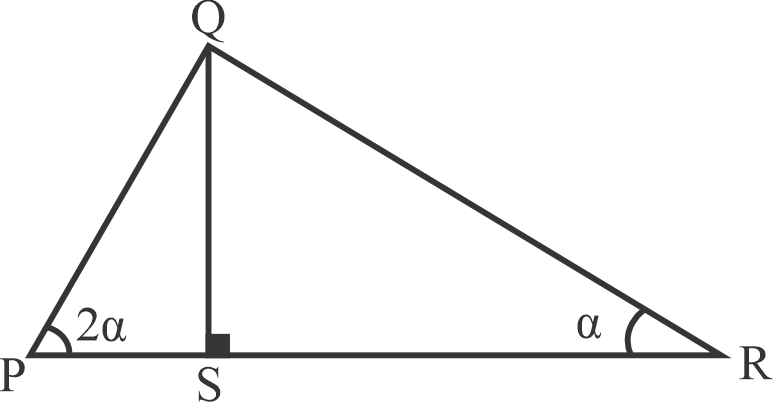
\includegraphics[width=4.5cm]{imagenes/CEPRE-UNA2024-I/etapa2/soc/geo1c24-I.png}
\end{center}
	
	\begin{enumerate}[label=\alph*)]
		\item 5
		\item 6
		\item 7
		\item 8
		\item 9
	\end{enumerate}
	\textbf{Respuesta correcta:} b)
	
	\vspace{2mm}
	\textbf{Solucionario:}\\[1mm]
	
	
		\begin{center}
		\begin{minipage}{0.45\textwidth}
			
			Se traza $QH$, del que $\text{m}\angle MQR=\text{m}\angle MRP \Rightarrow \triangle MQR$ es isósceles.
			
			$QM=MR$
			
			$x+3=9$
			
			\fbox{$x=6$}

			\vspace{6mm}
		\end{minipage}
		\hfill
		\begin{minipage}{0.45\textwidth}
			\centering
			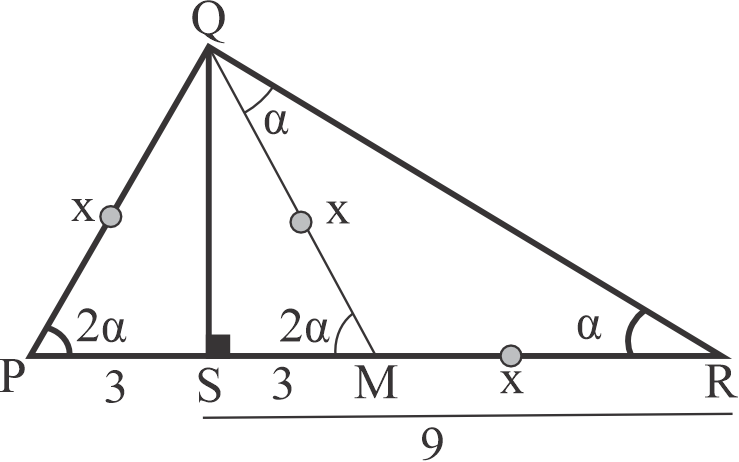
\includegraphics[width=4.5cm]{imagenes/CEPRE-UNA2024-I/etapa2/soc/geo1c24-Ir.png}
		\end{minipage}
	\end{center}
	
	
	
	
	
	
	\vspace{6mm}
	
	\item Halle el perímetro del triángulo $ABC$.
	
	\begin{center}
		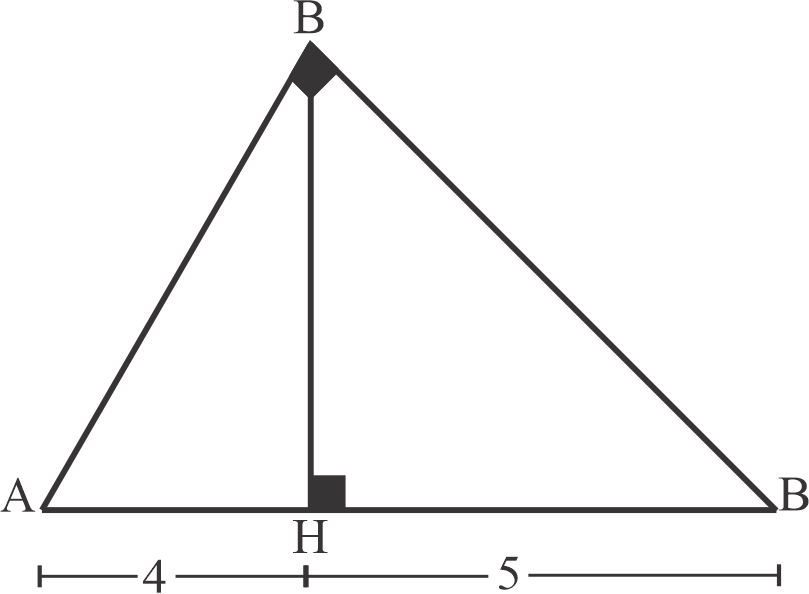
\includegraphics[width=4cm]{imagenes/CEPRE-UNA2024-I/etapa2/soc/geo2c24-I.png}
	\end{center}
	
	\begin{enumerate}[label=\alph*)]
		\item 4
		\item 5
		\item $\sqrt{5}$
		\item 3
		\item $3(5+\sqrt{5})$
	\end{enumerate}
	\textbf{Respuesta correcta:} e)
	
	\vspace{2mm}
	\textbf{Solucionario:}\\[1mm]
	
	Por propiedad:
	
	$x^2=4(9)=36$
	
	$x=6$
	
	$y^2=5(9)=45$
	
	$y=\sqrt{45}$
	
	Entonces el perímetro:
	
	$P=x+y+9=6+\sqrt{45}+9=15+3\sqrt{5}=$\fbox{$3(5+\sqrt{5})$}
	
	\vspace{6mm}
\end{enumerate}

\subsection*{Trigonometría}

\begin{enumerate}[resume]

	
	\item En un sector circular, el ángulo central mide $50^{g}$ y el radio mide $72\,cm$. ¿Cuánto mide la longitud de su arco?
	\begin{enumerate}[label=\alph*)]
		\item $12\pi\,cm$
		\item $16\pi\,cm$
		\item $18\pi\,cm$
		\item $20\pi\,cm$
		\item $36\pi\,cm$
	\end{enumerate}
	\textbf{Respuesta correcta:} c)
	
	\vspace{2mm}
	\textbf{Solucionario:}\\[1mm]
	
	\begin{center}
		\begin{tikzpicture}[scale=0.7]
			\coordinate (O) at (0,0);
			\coordinate (A) at (4.8,1.7);
			\coordinate (B) at (4.8,-1.7);
			
			\draw[thick] (O)--(A);
			\draw[thick] (O)--(B);
			\draw[thick] (A) arc[start angle=20,end angle=-20,radius=5.1];
			
			\node[left] at (2.5,0) {$\theta=50^g$};
			\node[above] at ($(O)!0.63!(A)$) {$R=72\,\text{cm}$};
			\node[right] at (5.3,0) {$L$};
		\end{tikzpicture}
	\end{center}
	
	$\theta=50^g=\dfrac{50\pi}{200}$
	
	$=\dfrac{5\pi}{20}$
	
	$=\dfrac{\pi}{4}\,\text{rad}$
	
	$L=\theta R$
	
	$=\dfrac{\pi}{4}(72)$
	
	$=\dfrac{\pi}{4}(4)(18)$
	
	\fbox{$L=18\pi\,\text{cm}$}
	
	\vspace{6mm}
	
	\item Si se cumple $\sen(5x+21^{\circ})=\cos(2x+6^{\circ})$, calcule el valor de $M=\tan x\,\cot 9^{\circ}+\tan 5x$.
	\begin{enumerate}[label=\alph*)]
		\item 2
		\item 3
		\item 4
		\item 5
		\item 6
	\end{enumerate}
	\textbf{Respuesta correcta:} a)
	
	\vspace{2mm}
	\textbf{Solucionario:}\\[1mm]
	Como:
	
	$\sen(5x+21^\circ)=\cos(2x+6^\circ)$
	
	$\Rightarrow 5x+21^\circ+2x+6^\circ=90^\circ$
	
	$7x+27^\circ=90^\circ$
	
	$7x=90^\circ-27^\circ$
	
	$7x=63^\circ$
	
	$x=9^\circ$
	
	Luego:
	
	$M=\tan 9^\circ\cdot \cot 9^\circ+\tan 5(9^\circ)$
	
	$=1+\tan 45^\circ$
	
	$=1+1$
	
	\fbox{$M=2$}
	
	\vspace{6mm}
\end{enumerate}

\subsection*{Física}

\begin{enumerate}[resume]

	
	\item Si el bloque es jalado por una fuerza $\vec F$ de magnitud $80\,N$ durante 8 segundos desde el punto $A$ hasta el punto $B$, halle la potencia que desarrolla la fuerza $\vec F$.
	
	\begin{center}
			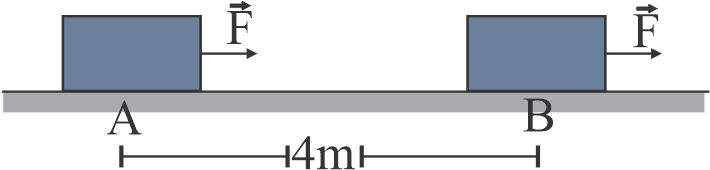
\includegraphics[width=5.5cm]{imagenes/CEPRE-UNA2024-I/etapa2/soc/fisica1c24-I.png}
	\end{center}
	
	\begin{enumerate}[label=\alph*)]
		\item 20 W
		\item 40 W
		\item 60 W
		\item 80 W
		\item 100 W
	\end{enumerate}
	\textbf{Respuesta correcta:} b)
	
	\vspace{2mm}
	\textbf{Solucionario:}\\[1mm]
	Trabajo realizado:
	
	$W=F\cdot d=80\cdot 4=320\,J$.
	
	Potencia media:
	
	$P=\dfrac{W}{t}=\dfrac{320}{8}=$\fbox{$40\,W$}
	
	\vspace{6mm}
	
	\item Calcule la presión hidrostática que ejerce el agua en el fondo del pozo mostrado. $(g=10\,m/s^2)$
	
	\begin{center}
		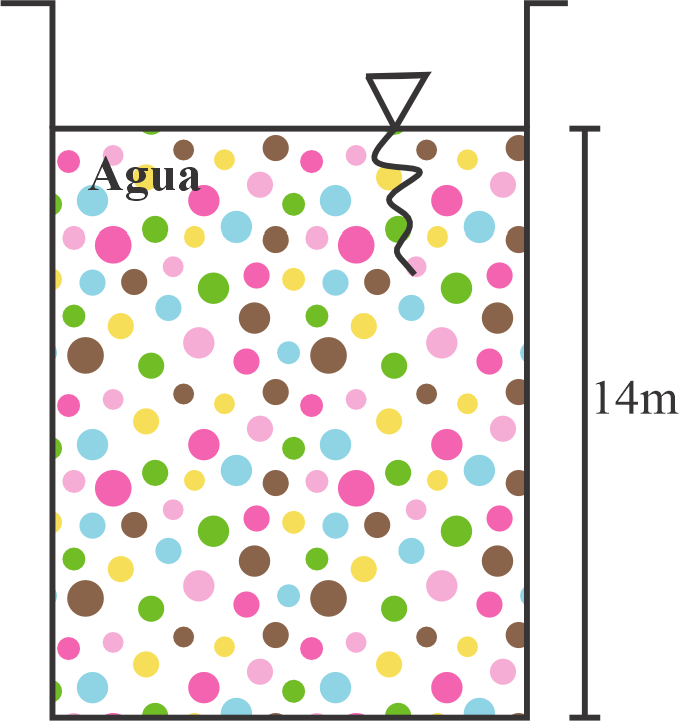
\includegraphics[width=4cm]{imagenes/CEPRE-UNA2024-I/etapa2/soc/fisica2c24-I.png}
	\end{center}
	
	\begin{enumerate}[label=\alph*)]
		\item 120 kPa
		\item 140 kPa
		\item 160 kPa
		\item 180 kPa
		\item 100 kPa
	\end{enumerate}
	\textbf{Respuesta correcta:} b)
	
	\vspace{2mm}
	\textbf{Solucionario:}\\[1mm]
	La presión hidrostática es:
	
	$P=\rho gh=1000\cdot 10\cdot 14=140000\,Pa=$\fbox{$140\,kPa$}
	
	\vspace{6mm}
\end{enumerate}

\subsection*{Química}

\begin{enumerate}[resume]

	\item ¿Cuántos gramos de oxígeno se encuentran en 800 gramos de $CaCO_3$?
	
	$(PA:\; Ca=40;\; C=12;\; O=16)$
	\begin{enumerate}[label=\alph*)]
		\item 280 g
		\item 320 g
		\item 384 g
		\item 260 g
		\item 150 g
	\end{enumerate}
	\textbf{Respuesta correcta:} c)
	
	\vspace{2mm}
	\textbf{Solucionario:}\\[1mm]
	Masa molar del $CaCO_3$:
	
	$40+12+3(16)=100$.
	
	La masa del oxígeno en 1 mol es $48\,g$, es decir, el $48\%$ del compuesto.
	
	Entonces, en $800\,g$ habrá:
	
	$800\times 0.48=$\fbox{$384\,g$}
	
	\vspace{6mm}
	
	\item Ordene en forma ascendente, según su radio iónico, las especies iónicas:
	
	${}_{25}Mn^{2+},\; {}_{23}V^{2+},\; {}_{22}Ti^{2+},\; {}_{28}Ni^{2+}$
	
	\begin{enumerate}[label=\alph*)]
		\item ${}_{28}Ni^{2+} \,<\, {}_{23}V^{2+} \,<\, {}_{22}Ti^{2+} \,<\, {}_{23}Mn^{2+}$
		\item ${}_{23}V^{2+} \,<\, {}_{22}Ti^{2+} \,<\, {}_{28}Ni^{2+} \,<\, {}_{23}Mn^{2+}$
		\item ${}_{23}Mn^{2+} \,<\, {}_{28}Ni^{2+} \,<\, {}_{23}V^{2+} \,<\, {}_{22}Ti^{2+}$
		\item ${}_{28}Ni^{2+} \,<\, {}_{25}Mn^{2+} \,<\, {}_{23}V^{2+} \,<\, {}_{22}Ti^{2+}$
		\item ${}_{25}Mn^{2+} \,<\, {}_{28}Ni^{2+} \,<\, {}_{23}V^{2+} \,<\, {}_{22}Ti^{2+}$
	\end{enumerate}
	\textbf{Respuesta correcta:} d)
	
	\vspace{2mm}
	\textbf{Solucionario:}\\[1mm]
	Para cationes de una misma serie, al aumentar la carga nuclear efectiva, el radio tiende a disminuir.
	
	Entre estas especies, el menor radio corresponde a $Ni^{2+}$ y el mayor a $Ti^{2+}$.
	
	El orden ascendente es:
	
	
	\fbox{${}_{28}Ni^{2+} \,<\, {}_{25}Mn^{2+} \,<\, {}_{23}V^{2+} \,<\, {}_{22}Ti^{2+}$}
	
	\vspace{6mm}
\end{enumerate}

\subsection*{Biología y Anatomía}

\begin{enumerate}[resume]

	
	\item Las aletas del pez y de la ballena presentan semejanzas externas. Esto permite catalogarlas como órganos:
	\begin{enumerate}[label=\alph*)]
		\item vestigiales.
		\item atávicos.
		\item homólogos.
		\item rudimentarios.
		\item análogos.
	\end{enumerate}
	\textbf{Respuesta correcta:} e)
	
	\vspace{2mm}
	\textbf{Solucionario:}\\[1mm]
	Son órganos \textbf{análogos}, porque cumplen función semejante y presentan similitud externa, pero tienen distinto origen evolutivo.
	

	
	\vspace{6mm}
	
	\item ¿Qué tipo de tejido muscular encontramos en el tubo digestivo y vías urinarias?
	\begin{enumerate}[label=\alph*)]
		\item Cardíaco
		\item Esquelético
		\item Liso
		\item Voluntario
		\item Estriado
	\end{enumerate}
	\textbf{Respuesta correcta:} c)
	
	\vspace{2mm}
	\textbf{Solucionario:}\\[1mm]
	En las paredes del tubo digestivo y de las vías urinarias predomina el músculo \textbf{liso}, de contracción involuntaria.
	

	\vspace{6mm}
\end{enumerate}

\subsection*{Psicología y Filosofía}

\begin{enumerate}[resume]

	
	\item Cuando afirmamos que Sonia es individual e incomparable en su forma de llegar al conocimiento de su entorno, ¿qué característica de la conciencia se manifiesta?
	\begin{enumerate}[label=\alph*)]
		\item Subjetiva
		\item Temporal
		\item Múltiple
		\item Unitaria
		\item Prospectiva
	\end{enumerate}
	\textbf{Respuesta correcta:} a)
	
	\vspace{2mm}
	\textbf{Solucionario:}\\[1mm]
	La conciencia es \textbf{subjetiva} porque cada persona conoce y experimenta la realidad desde su propia individualidad.
	
	
	
	\vspace{6mm}
	
	\item Guillermo sostiene: ``Si la realidad es dinámica entonces el conocimiento, reflejo de la realidad, también lo es''. Expresa una tesis:
	\begin{enumerate}[label=\alph*)]
		\item metafísica.
		\item fenomenista.
		\item escepticista.
		\item realista.
		\item criticista.
	\end{enumerate}
	\textbf{Respuesta correcta:} d)
	
	\vspace{2mm}
	\textbf{Solucionario:}\\[1mm]
	La afirmación considera que el conocimiento refleja la realidad objetiva; eso corresponde a una postura \textbf{realista}.
	

	
	\vspace{6mm}
	
	\item Un estudiante narra que, cuando lo asaltaron, sintió un aumento del ritmo cardíaco y no podía respirar. Esto sería un ejemplo de proceso afectivo de:
	\begin{enumerate}[label=\alph*)]
		\item amplitud.
		\item polaridad.
		\item intimidad.
		\item intensidad.
		\item profundidad.
	\end{enumerate}
	\textbf{Respuesta correcta:} d)
	
	\vspace{2mm}
	\textbf{Solucionario:}\\[1mm]
	La emoción se manifiesta con gran fuerza fisiológica; por ello corresponde a la \textbf{intensidad} del proceso afectivo.
	
	
	
	\vspace{6mm}
	
	\item Es el movimiento psicológico que surgió a mediados del siglo XX y asumió una postura opuesta al determinismo del psicoanálisis, así como al mecanicismo del conductismo y constituyó la tercera fuerza de la psicología.
	\begin{enumerate}[label=\alph*)]
		\item Estructuralismo
		\item Psicogenética
		\item Cognitivismo
		\item Funcionalismo
		\item Humanismo
	\end{enumerate}
	\textbf{Respuesta correcta:} e)
	
	\vspace{2mm}
	\textbf{Solucionario:}\\[1mm]
	La ``tercera fuerza'' de la psicología es el \textbf{humanismo}, que valora la libertad, la autorrealización y la experiencia humana.
	

	
	\vspace{6mm}
\end{enumerate}

\subsection*{Geografía}

\begin{enumerate}[resume]

	
	\item La pesca, minería, explotación forestal, caza y recolección, son actividades:
	\begin{enumerate}[label=\alph*)]
		\item extractivas.
		\item productivas.
		\item transformativas.
		\item de servicios.
		\item agropecuarios.
	\end{enumerate}
	\textbf{Respuesta correcta:} a)
	
	\vspace{2mm}
	\textbf{Solucionario:}\\[1mm]
	Son actividades \textbf{extractivas} porque obtienen directamente los recursos de la naturaleza.
	

	
	\vspace{6mm}
	
	\item La central hidroeléctrica Santiago Antúnez de Mayolo se localiza en la cuenca del río:
	\begin{enumerate}[label=\alph*)]
		\item Ene.
		\item Mantaro.
		\item Urubamba.
		\item Ucayali.
		\item Tambo.
	\end{enumerate}
	\textbf{Respuesta correcta:} b)
	
	\vspace{2mm}
	\textbf{Solucionario:}\\[1mm]
	La central Santiago Antúnez de Mayolo forma parte del complejo hidroeléctrico del río \textbf{Mantaro}.
	
	
	\vspace{6mm}
	
	\item Es el río que desagua en la parte norte de la bahía de Chucuito y se forma por afluencia de los ríos Lampa y Cabanillas.
	\begin{enumerate}[label=\alph*)]
		\item Coata
		\item Ramis
		\item Suches
		\item Ilave
		\item Huancané - Putina
	\end{enumerate}
	\textbf{Respuesta correcta:} a)
	
	\vspace{2mm}
	\textbf{Solucionario:}\\[1mm]
	El río formado por los ríos Lampa y Cabanillas es el \textbf{Coata}, que desemboca en la parte norte de la bahía de Chucuito.
	
	
	
	\vspace{6mm}
	
	\item Son los vientos que soplan de manera constante en verano, van desde las altas presiones subtropicales hacia las bajas presiones ecuatoriales y soplan de noreste al sudeste en el hemisferio norte y del sudeste al noreste en el hemisferio sur.
	\begin{enumerate}[label=\alph*)]
		\item Polares
		\item Brisas
		\item Ciclones
		\item Alisios
		\item Contralisios
	\end{enumerate}
	\textbf{Respuesta correcta:} d)
	
	\vspace{2mm}
	\textbf{Solucionario:}\\[1mm]
	La descripción corresponde a los \textbf{vientos alisios}, que soplan constantemente desde zonas subtropicales hacia la franja ecuatorial.
	

	
	\vspace{6mm}
\end{enumerate}

\subsection*{Historia}

\begin{enumerate}[resume]

	
	\item En el origen mitológico de la cultura Lambayeque existe un personaje legendario denominado Naylamp. Algo similar acontece en la cultura Chimú, donde también aparece un personaje mítico llamado:
	\begin{enumerate}[label=\alph*)]
		\item Chimú Cápac.
		\item Tacaynamo.
		\item Gran Chimú.
		\item Michan Caman.
		\item Murcahn Zaman.
	\end{enumerate}
	\textbf{Respuesta correcta:} b)
	
	\vspace{2mm}
	\textbf{Solucionario:}\\[1mm]
	El personaje mítico de origen en la cultura Chimú es \textbf{Tacaynamo}.
	

	
	\vspace{6mm}
	
	\item En el período conocido como el Oncenio de Augusto B. Leguía, se recuerda un hecho importante para la historia:
	\begin{enumerate}[label=\alph*)]
		\item la celebración del centenario de la independencia del Perú (28 de julio de 1921).
		\item el surgimiento del primer partido civil del Perú.
		\item el sesquicentenario de la independencia política.
		\item el cincuentenario de la república aristocrática.
		\item la creación de los consejos regionales eliminando a las juntas departamentales.
	\end{enumerate}
	\textbf{Respuesta correcta:} a)
	
	\vspace{2mm}
	\textbf{Solucionario:}\\[1mm]
	Durante el Oncenio de Leguía se celebró el \textbf{centenario de la independencia} en 1921.
	

	
	\vspace{6mm}
	
	\item En el gobierno de Manuel A. Odría (1950--1956), se creó un organismo encargado de estudios geopolíticos y militares denominado:
	\begin{enumerate}[label=\alph*)]
		\item Comando Conjunto de las Fuerzas Armadas.
		\item Consejo de Militares.
		\item Servicio Nacional de Inteligencia.
		\item Instituto Peruano de Estudios Geopolíticos.
		\item Centro de Altos Estudios Militares.
	\end{enumerate}
	\textbf{Respuesta correcta:} e)
	
	\vspace{2mm}
	\textbf{Solucionario:}\\[1mm]
	Durante ese gobierno se creó el \textbf{Centro de Altos Estudios Militares (CAEM)}.
	

	
	\vspace{6mm}
	
	\item El líder militar que se sublevó en defensa de los campesinos del departamento de Puno en la segunda década del siglo XX fue:
	\begin{enumerate}[label=\alph*)]
		\item Zacarias Puntaca Farfán.
		\item José Antonio Salazar Huilca.
		\item Juan Dueñas Bustamante.
		\item Teodomiro Gutiérrez Cuevas.
		\item José Gabriel Condorcanqui.
	\end{enumerate}
	\textbf{Respuesta correcta:} d)
	
	\vspace{2mm}
	\textbf{Solucionario:}\\[1mm]
	El militar vinculado a la rebelión en defensa de campesinos puneños fue \textbf{Teodomiro Gutiérrez Cuevas}, conocido también como Rumi Maqui.
	

	
	\vspace{6mm}
\end{enumerate}

\subsection*{Educación Cívica}

\begin{enumerate}[resume]

	
	\item David, estudiante universitario, asistió a una ponencia y escuchó la siguiente expresión: ``El sentido de pertenencia vincula a todo individuo con un grupo humano, social y cultural''. Del texto podemos afirmar que la ponencia trató sobre la:
	\begin{enumerate}[label=\alph*)]
		\item tolerancia.
		\item tradición.
		\item igualdad.
		\item identidad.
		\item cosmovisión.
	\end{enumerate}
	\textbf{Respuesta correcta:} d)
	
	\vspace{2mm}
	\textbf{Solucionario:}\\[1mm]
	El sentido de pertenencia a un grupo humano y cultural define la \textbf{identidad}.
	

	
	\vspace{6mm}
	
	\item Mantener comunicación con las organizaciones sociales, proponer proyectos de ordenanza municipal y desempeñar funciones de fiscalización de la gestión municipal, son atribuciones que corresponden:
	\begin{enumerate}[label=\alph*)]
		\item al alcalde.
		\item a los consejeros municipales.
		\item al teniente alcalde.
		\item a los regidores.
		\item al gerente municipal.
	\end{enumerate}
	\textbf{Respuesta correcta:} d)
	
	\vspace{2mm}
	\textbf{Solucionario:}\\[1mm]
	Esas funciones corresponden a los \textbf{regidores}, quienes integran el concejo municipal y fiscalizan la gestión.
	

	
	\vspace{6mm}
	
	\item \rule{2cm}{0.15mm} es un organismo constitucionalmente autónomo cuya función es velar por el uso adecuado de los recursos públicos. Y su representante es designado por \rule{2cm}{0.15mm}, a propuesta del Presidente de la República.
	\begin{enumerate}[label=\alph*)]
		\item La Contraloría General de la República -- la Comisión Extraordinaria.
		\item El Ministerio Público -- la Contraloría General de la República.
		\item La Contraloría General de la República -- el Congreso de la República.
		\item La Defensoría del Pueblo -- el Congreso de la República.
		\item La SUNAT -- el Ministerio Público.
	\end{enumerate}
	\textbf{Respuesta correcta:} c)
	
	\vspace{2mm}
	\textbf{Solucionario:}\\[1mm]
	El organismo es la \textbf{Contraloría General de la República}.
	
	El contralor es designado por el \textbf{Congreso de la República}, a propuesta del Presidente.
	

	
	\vspace{6mm}
	
	\item Es el órgano competente para declarar la vacancia del Gobernador Regional.
	\begin{enumerate}[label=\alph*)]
		\item La Gerencia Regional
		\item La Sociedad Civil
		\item La Presidencia Regional
		\item El Concejo de Coordinación Regional
		\item El Consejo Regional
	\end{enumerate}
	\textbf{Respuesta correcta:} e)
	
	\vspace{2mm}
	\textbf{Solucionario:}\\[1mm]
	La vacancia del gobernador regional corresponde al \textbf{Consejo Regional}.
	

	
	\vspace{6mm}
\end{enumerate}

\subsection*{Economía}

\begin{enumerate}[resume]

	
	\item La abogada Karla obtiene rentas por el ejercicio profesional independiente en su estudio jurídico. ¿A qué categoría del Impuesto a la Renta pertenece?
	\begin{enumerate}[label=\alph*)]
		\item Primera categoría
		\item Segunda categoría
		\item Tercera categoría
		\item Cuarta categoría
		\item Quinta categoría
	\end{enumerate}
	\textbf{Respuesta correcta:} d)
	
	\vspace{2mm}
	\textbf{Solucionario:}\\[1mm]
	El ejercicio profesional independiente genera rentas de \textbf{cuarta categoría}.
	

	
	\vspace{6mm}
	
	\item La Ley de Gresham establece que:
	\begin{enumerate}[label=\alph*)]
		\item las monedas de metal precioso son más valiosas que las de papel.
		\item las personas prefieren guardar sus monedas valiosas en lugar de gastarlas.
		\item el valor de las monedas se mide por su valor real.
		\item las monedas y billetes constituyen la emisión primaria.
		\item las monedas ``malas'' tienden a desplazar del mercado a las monedas ``buenas''.
	\end{enumerate}
	\textbf{Respuesta correcta:} e)
	
	\vspace{2mm}
	\textbf{Solucionario:}\\[1mm]
	La Ley de Gresham resume la idea de que la \textbf{moneda mala desplaza a la buena} cuando ambas circulan con el mismo valor nominal.
	

	
	\vspace{6mm}
	
	\item Seleccione la opción que mejor define el presupuesto público.
	\begin{enumerate}[label=\alph*)]
		\item Incluye todos los ingresos de fuente tributaria.
		\item Incluye todos los ingresos y gastos que el gobierno prevé y planifica para un período anual.
		\item Incluye todos los ingresos e inversiones de los ciudadanos.
		\item Representa la cantidad de dinero que el gobierno peruano presta a otros países.
		\item Se refiere únicamente a los fondos destinados a la educación pública en el Perú.
	\end{enumerate}
	\textbf{Respuesta correcta:} b)
	
	\vspace{2mm}
	\textbf{Solucionario:}\\[1mm]
	El presupuesto público es el instrumento que contiene los \textbf{ingresos y gastos previstos por el Estado para un año fiscal}.
	

	
	\vspace{6mm}
	
	\item En su conjunto, el mercado de trabajo, el mercado de capitales y el mercado de recursos forman el llamado:
	\begin{enumerate}[label=\alph*)]
		\item mercado de recursos.
		\item mercado laboral.
		\item mercado financiero.
		\item mercado de bienes.
		\item mercado de factores.
	\end{enumerate}
	\textbf{Respuesta correcta:} e)
	
	\vspace{2mm}
	\textbf{Solucionario:}\\[1mm]
	Trabajo, capital y recursos son \textbf{factores de producción}; por eso integran el mercado de factores.
	

	
	\vspace{6mm}
\end{enumerate}

\subsection*{Comunicación}

\begin{enumerate}[resume]

	
	\item Juan, mi sobrino, es muy agraciado. A pesar de sus veintidós años, tiene mucha madurez, razona sobre los conflictos sociales, es alegre y muy sabio. Tiene una voz exuberante y atractiva.
	
	El fragmento expresa una descripción de tipo:
	\begin{enumerate}[label=\alph*)]
		\item prosopografía.
		\item etopeya.
		\item caricatura.
		\item retrato.
		\item topografía.
	\end{enumerate}
	\textbf{Respuesta correcta:} d)
	
	\vspace{2mm}
	\textbf{Solucionario:}\\[1mm]
	La descripción mezcla rasgos físicos (voz, apariencia) y psicológicos o morales (madurez, alegría, sabiduría).
	
	Esa combinación constituye un \textbf{retrato}.
	

	
	\vspace{6mm}
	
	\item Los mensajes de función \rule{2cm}{0.15mm} son los que están destinados a abrir, mantener o interrumpir el contacto entre emisor y receptor.
	\begin{enumerate}[label=\alph*)]
		\item poética
		\item fática
		\item representativa
		\item metalingüística
		\item expresiva
	\end{enumerate}
	\textbf{Respuesta correcta:} b)
	
	\vspace{2mm}
	\textbf{Solucionario:}\\[1mm]
	La función del lenguaje que sirve para abrir, mantener o cerrar el canal de comunicación es la \textbf{fática}.
	

	
	\vspace{6mm}
	
	\item Un alumno pregunta al docente sobre la calidad del texto que escribió. Este le responde que el texto escrito presenta problemas de organización de la información.
	
	En la situación comunicativa, el docente observa en el texto escrito un problema de:
	\begin{enumerate}[label=\alph*)]
		\item cohesión.
		\item coherencia.
		\item adecuación.
		\item implicación.
		\item revisión.
	\end{enumerate}
	\textbf{Respuesta correcta:} b)
	
	\vspace{2mm}
	\textbf{Solucionario:}\\[1mm]
	La organización lógica de la información corresponde a la \textbf{coherencia}.
	
	Si falla, las ideas no guardan un orden claro.
	

	
	\vspace{6mm}
	
	\item Es una palabra o locución que sirve para expresar la relación gramatical y lógica entre dos proposiciones o entre dos elementos análogos de una oración.
	\begin{enumerate}[label=\alph*)]
		\item La preposición
		\item La conjunción
		\item El adverbio
		\item El artículo
		\item El pronombre
	\end{enumerate}
	\textbf{Respuesta correcta:} b)
	
	\vspace{2mm}
	\textbf{Solucionario:}\\[1mm]
	La palabra que enlaza proposiciones o términos análogos es la \textbf{conjunción}.
	

	
	\vspace{6mm}
\end{enumerate}

\subsection*{Literatura}

\begin{enumerate}[resume]

	
	\item En \textit{La metamorfosis} de Franz Kafka, el padre de Gregorio considera a su hijo un ser inservible para el mundo moderno porque:
	\begin{enumerate}[label=\alph*)]
		\item no se puede adaptar a una profesión tan agitada.
		\item no produce nada y es una vergüenza para la familia.
		\item hace pasar a la familia muchas penurias económicas.
		\item ha abandonado su trabajo cansado de la rutina.
		\item obliga a trabajar a los miembros de la familia.
	\end{enumerate}
	\textbf{Respuesta correcta:} b)
	
	\vspace{2mm}
	\textbf{Solucionario:}\\[1mm]
	Tras la transformación de Gregorio, el padre lo considera inútil e improductivo, además de motivo de vergüenza para la familia.
	
	Por eso la mejor opción es la \textbf{b)}.
	

	
	\vspace{6mm}
	
	\item La segunda parte de los \textit{Comentarios Reales} del Inca Garcilaso de la Vega se refiere a:
	\begin{enumerate}[label=\alph*)]
		\item la conquista y las guerras civiles entre españoles.
		\item la expedición de Hernando de Soto a la Florida.
		\item los recuerdos de la niñez y juventud del autor.
		\item los dioses y hombres que habitaron Huarochirí.
		\item los orígenes de la cultura e historia del pueblo inca.
	\end{enumerate}
	\textbf{Respuesta correcta:} a)
	
	\vspace{2mm}
	\textbf{Solucionario:}\\[1mm]
	La segunda parte de la obra aborda la \textbf{conquista del Perú y las guerras civiles entre españoles}.
	

	
	\vspace{6mm}
	
	\item En la novela \textit{El ingenioso hidalgo Don Quijote de la Mancha}, el final del protagonista se ve representado por el siguiente suceso:
	\begin{enumerate}[label=\alph*)]
		\item encuentra a Dulcinea y se casa con ella.
		\item se vuelve loco y es encerrado en un manicomio.
		\item recobra la razón y muere en casa.
		\item pierde la memoria y se extravía en la Mancha.
		\item enferma gravemente y se queda convaleciente.
	\end{enumerate}
	\textbf{Respuesta correcta:} c)
	
	\vspace{2mm}
	\textbf{Solucionario:}\\[1mm]
	Al final de la novela, don Quijote recupera la cordura, reniega de sus fantasías caballerescas y muere en su casa.
	

	
	\vspace{6mm}
	
	\item Al final de \textit{El Lazarillo de Tormes}, el protagonista:
	\begin{enumerate}[label=\alph*)]
		\item se encuentra con su madre.
		\item asume el oficio de caballero.
		\item se casa y es nombrado pregonero en Toledo.
		\item vuelve a encontrar al ciego.
		\item llega a ser rico y tiene su lazarillo.
	\end{enumerate}
	\textbf{Respuesta correcta:} c)
	
	\vspace{2mm}
	\textbf{Solucionario:}\\[1mm]
	Lázaro termina casado con la criada del arcipreste y ejerciendo como \textbf{pregonero en Toledo}.
	

	
	\vspace{6mm}
\end{enumerate}

\subsection*{Razonamiento Matemático}

\begin{enumerate}[resume]

	
	\item Complete las casillas en blanco con números de un dígito de manera que al sumar los valores de cada fila o columna resulten 34. ¿Cuántas veces aparece el dígito 9 en ambas diagonales?
	
	\begin{center}
		$
		\renewcommand{\arraystretch}{1.2}
		\begin{array}{|c|c|c|c|}
			\hline
			& 8 &  & 9 \\
			\hline
			8 &  &  &  \\
			\hline
			8 &  &  & 8 \\
			\hline
			&  & 9 &  \\
			\hline
		\end{array}
		$
	\end{center}
	
	\begin{enumerate}[label=\alph*)]
		\item 4
		\item 5
		\item 6
		\item 7
		\item 8
	\end{enumerate}
	\textbf{Respuesta correcta:} c)
	
	\vspace{2mm}
	\textbf{Solucionario:}\\[1mm]
	Sea la cuadrícula:
	
	$
	\begin{matrix}
		a&8&b&9\\
		8&c&d&e\\
		8&f&g&8\\
		h&i&9&j
	\end{matrix}
	$
	
	Imponiendo que cada fila y columna sume $34$ se obtiene una solución única:
	
	$
	\begin{matrix}
		9&8&8&9\\
		8&9&8&9\\
		8&9&9&8\\
		9&8&9&8
	\end{matrix}
	$
	
	Las diagonales son $9,9,9,8$ y $9,8,9,9$.
	
	En total, el dígito $9$ aparece $3+3=$	\fbox{$6$} veces.
	

	
	\vspace{6mm}
	
	\item Ana y Beatriz preparan pasteles. Si el triple de lo que prepara Ana más lo de Beatriz es mayor que 51 y el doble de Ana menos lo de Beatriz es 24. ¿Cuál es la cantidad mínima de pasteles que prepara Ana?
	\begin{enumerate}[label=\alph*)]
		\item 16
		\item 23
		\item 24
		\item 25
		\item 18
	\end{enumerate}
	\textbf{Respuesta correcta:} a)
	
	\vspace{2mm}
	\textbf{Solucionario:}\\[1mm]
	Sea $A$ lo de Ana y $B$ lo de Beatriz.
	
	Del dato:
	
	$2A-B=24$.
	
	$B=2A-24$.
	
	Sustituyendo en $3A+B>51$:
	
	$3A+(2A-24)>51$.
	
	$5A>75$.
	
	$A>15$.
	
	La cantidad mínima entera es $A=$\fbox{$16$}
	
	\vspace{6mm}
	
	\item Se define el operador $*$ en $\mathbb{N}$.
	A partir de la tabla:
	
	$
	\begin{array}{c|cccccc}
		* & 1 & 2 & 3 & 4 & \cdots \\
		\hline
		1 & 1 & 2 & 3 & 4 & \\
		2 & 2 & 3 & 4 & 5 & \\
		3 & 3 & 4 & 5 & 6 & \\
		4 & 4 & 5 & 6 & 7 & \\
		\vdots & & & & & &
	\end{array}
	$
	
	halle $(6*7)*(3*5)$
	\begin{enumerate}[label=\alph*)]
		\item 19
		\item 17
		\item 18
		\item 20
		\item 16
	\end{enumerate}
	\textbf{Respuesta correcta:} c)
	
	\vspace{2mm}
	\textbf{Solucionario:}\\[1mm]
	De la tabla se deduce la regla:
	
	$a*b=a+b-1$.
	
	Entonces:
	
	$6*7=6+7-1=12$.
	
	$3*5=3+5-1=7$.
	
	Por tanto:
	
	$(6*7)*(3*5)=12*7=12+7-1=$\fbox{$18$}
	
	\vspace{6mm}
	
	\item En el gráfico, tomando como centro de la circunferencia a $C$, se ha trazado el arco $\widehat{AD}$. Si $AB$ es diámetro del semicírculo, $AB=BC=2\,cm$ y $CD=DE$, calcule el perímetro de la región sombreada.
	
	\begin{center}
		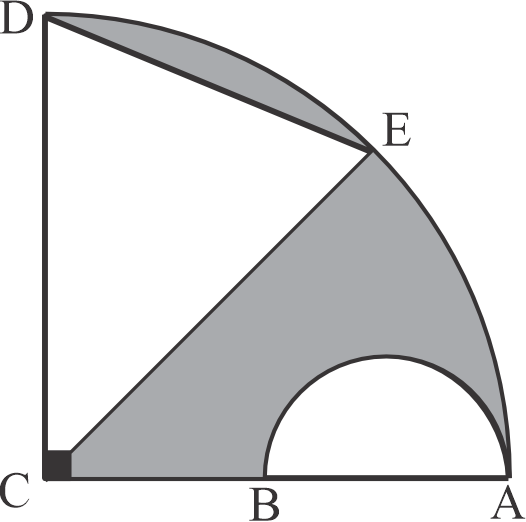
\includegraphics[width=3.2cm]{imagenes/CEPRE-UNA2024-I/etapa2/soc/rm4c24-I.png}
	\end{center}
	
	\begin{enumerate}[label=\alph*)]
		\item $(8+3\pi)\,cm$
		\item $(9+2\pi)\,cm$
		\item $(10+3\pi)\,cm$
		\item $\left(8+\dfrac{5\pi}{2}\right)\,cm$
		\item $(7+\pi)\,cm$
	\end{enumerate}
	\textbf{Respuesta correcta:} c)
	
	\vspace{2mm}
	\textbf{Solucionario:}\\[1mm]
	Como $AB=BC=2$, entonces $CA=4$ y el cuarto de circunferencia tiene radio $4$.
	
	Además, $CD=4$ y por dato $DE=4$.
	
	El arco total $\widehat{DA}$ del cuarto de circunferencia mide:
	
	$L_1=\dfrac{1}{4}(2\pi\cdot 4)=2\pi$.
	
	El semicírculo tiene radio $1$, así que su arco mide:
	
	$L_2=\pi$.
	
	Los segmentos rectos del contorno sombreado son $DE=4$, $CE=4$ y $CB=2$.
	
	Entonces el perímetro total es:
	
	$P=2\pi+\pi+4+4+2=$\fbox{$10+3\pi$}
	
	\vspace{6mm}
	
	\item Definimos el operador
	
	$\boxed{2x+1}=4x+7$
	
	Halle el valor de $\boxed{8}$
	\begin{enumerate}[label=\alph*)]
		\item 17
		\item 18
		\item 35
		\item 21
		\item 25
	\end{enumerate}
	\textbf{Respuesta correcta:} d)
	
	\vspace{2mm}
	\textbf{Solucionario:}\\[1mm]
	Sea $\boxed{y}=f(y)$.
	
	Dado que si $y=2x+1$, entonces:
	
	$f(y)=4x+7=2(2x+1)+5=2y+5$.
	
	Por tanto:
	
	$\boxed{8}=2(8)+5=$\fbox{$21$}
	
	\vspace{6mm}
	
	\item Determine $x+y$ si
	
	\begin{center}
		\begin{tikzpicture}[scale=0.38]
			\draw[very thick] (0,0) circle (3);
			
			\draw[very thick] (0,0) -- (0,3);
			\draw[very thick] (0,0) -- (2.12,2.12);
			\draw[very thick] (0,0) -- (3,0);
			\draw[very thick] (0,0) -- (2.12,-2.12);
			\draw[very thick] (0,0) -- (0,-3);
			\draw[very thick] (0,0) -- (-2.12,-2.12);
			\draw[very thick] (0,0) -- (-3,0);
			\draw[very thick] (0,0) -- (-2.12,2.12);
			
			\node at (1.05,2.25) {$7$};
			\node at (2.15,1.05) {$11$};
			\node at (1.8,-0.85) {$5$};
			\node at (1.0,-2.05) {$8$};
			\node at (-0.9,-2.05) {$13$};
			\node at (-1.8,-0.85) {$y$};
			\node at (-2.05,1.0) {$x$};
			\node at (-1.0,2.15) {$4$};
		\end{tikzpicture}
	\end{center}
	
	\begin{enumerate}[label=\alph*)]
		\item 17
		\item 18
		\item 20
		\item 24
		\item 26
	\end{enumerate}
	\textbf{Respuesta correcta:} e) 
	
	\vspace{2mm}
	\textbf{Solucionario:}\\[1mm]
	
	\begin{center}
		\begin{tikzpicture}[scale=0.38]
			\draw[very thick] (0,0) circle (3);
			
			\draw[very thick] (0,0) -- (0,3);
			\draw[very thick] (0,0) -- (2.12,2.12);
			\draw[very thick] (0,0) -- (3,0);
			\draw[very thick] (0,0) -- (2.12,-2.12);
			\draw[very thick] (0,0) -- (0,-3);
			\draw[very thick] (0,0) -- (-2.12,-2.12);
			\draw[very thick] (0,0) -- (-3,0);
			\draw[very thick] (0,0) -- (-2.12,2.12);
			
			\node at (1.05,2.25) {$7$};
			\node at (2.15,1.05) {$11$};
			\node at (1.8,-0.85) {$5$};
			\node at (1.0,-2.05) {$8$};
			\node at (-0.9,-2.05) {$13$};
			\node at (-1.8,-0.85) {$y$};
			\node at (-2.05,1.0) {$x$};
			\node at (-1.0,2.15) {$4$};
		\end{tikzpicture}
	\end{center}
	
	La suma de $4+7=11$ \\
	La suma de $11+5=16$ \\
	La suma de $8+13=21$\\
	La suma de $y+x=?$  \\
	
	
	$11,16,21,?$ la diferencia entre estas es 5 
	
	por lo tanto  $y+x=21+5=$\fbox{$26$}
	\vspace{6mm}
\end{enumerate}

\subsection*{Razonamiento Verbal}

\begin{enumerate}[resume]

	
	\item En la palabra \textbf{ABSTEMIO}, el prefijo \textbf{ABS} significa:
	\begin{enumerate}[label=\alph*)]
		\item condenación.
		\item construcción.
		\item separación.
		\item inferencia.
		\item relación.
	\end{enumerate}
	\textbf{Respuesta correcta:} c)
	
	\vspace{2mm}
	\textbf{Solucionario:}\\[1mm]
	El prefijo latino \textbf{abs-} expresa idea de alejamiento o \textbf{separación}.
	
	Por eso ``abstemio'' alude a quien se aparta de beber alcohol.
	

	
	\vspace{6mm}
	
	\item Para la universidad, la excelencia académica significa lograr una educación \rule{1cm}{0.15mm} forma profesionales competentes y éticos, \rule{1cm}{0.15mm} aporten al desarrollo del país.
	\begin{enumerate}[label=\alph*)]
		\item que - quienes
		\item cuando - mientras
		\item donde - pero
		\item cual - cuyos
		\item cuyo - más
	\end{enumerate}
	\textbf{Respuesta correcta:} a)
	
	\vspace{2mm}
	\textbf{Solucionario:}\\[1mm]
	La forma correcta es: ``una educación \textbf{que} forma profesionales competentes y éticos, \textbf{quienes} aporten al desarrollo del país''.
	

	
	\vspace{6mm}
	
	\item El antónimo de la palabra \textbf{ALEVOSÍA} es:
	\begin{enumerate}[label=\alph*)]
		\item felonía.
		\item perfidia.
		\item traición.
		\item condición.
		\item lealtad.
	\end{enumerate}
	\textbf{Respuesta correcta:} e)
	
	\vspace{2mm}
	\textbf{Solucionario:}\\[1mm]
	``Alevosía'' se relaciona con traición o perfidia; su antónimo es \textbf{lealtad}.
	

	
	\vspace{6mm}
	
	\item El sinónimo de la palabra \textbf{LACÓNICO} es:
	\begin{enumerate}[label=\alph*)]
		\item breve.
		\item enjuto.
		\item parco.
		\item agotado.
		\item caviloso.
	\end{enumerate}
	\textbf{Respuesta correcta:} a)
	
	\vspace{2mm}
	\textbf{Solucionario:}\\[1mm]
	``Lacónico'' significa breve, conciso, de pocas palabras.
	
	La opción más directa es \textbf{breve}.
	

	
	\vspace{6mm}
	
	\item \textbf{PLAN DE REDACCIÓN}
	
	I. Ahora que he ingresado, me toca estudiar para hacer realidad mi carrera.\\
	II. He concluido mi secundaria, soy uno de los 260 000 estudiantes que egresan cada año.\\
	III. De antemano, sé que la competencia es dura, por eso me he preparado a conciencia.\\
	IV. Deseo seguir mis estudios en una buena universidad, la mejor de todas.\\
	V. Di mi examen y respondí todas las preguntas que sabía.
	
	\begin{enumerate}[label=\alph*)]
		\item II -- IV -- I -- V -- III
		\item II -- III -- I -- IV -- V
		\item I -- II -- V -- IV -- III
		\item II -- IV -- III -- V -- I
		\item II -- IV -- I -- III -- V
	\end{enumerate}
	\textbf{Respuesta correcta:} d)
	
	\vspace{2mm}
	\textbf{Solucionario:}\\[1mm]
	El orden lógico es: primero concluye la secundaria (II), luego expresa su deseo de seguir estudios (IV), después reconoce la competencia y se prepara (III), luego da el examen (V) y finalmente, al ingresar, se proyecta a estudiar la carrera (I).
	

	
	\vspace{6mm}
	
	\item \textbf{COMPRENSIÓN DE TEXTO}
	
	\begin{quote}
		Soy otro cuando soy; los actos míos son más míos\\
		si son también de todos, para que pueda ser, he\\
		de ser otro, salir de mí, buscarme entre los otros.
	\end{quote}
	\hfill Octavio Paz
	
	¿Cuál es la intención del autor?
	\begin{enumerate}[label=\alph*)]
		\item Mostrarse como otro.
		\item Evitar ser confundido con los otros.
		\item Argumentar sobre la referencia colectiva del ser humano.
		\item Evidenciar las semejanzas entre unos y otros.
		\item Hablar sobre la identidad del hombre.
	\end{enumerate}
	\textbf{Respuesta correcta:} c)
	
	\vspace{2mm}
	\textbf{Solucionario:}\\[1mm]
	Octavio Paz argumenta que el individuo se realiza plenamente solo en relación con los demás.
	
	La frase \textit{``los actos míos son más míos si son también de todos''} evidencia que la intención central es destacar la \textbf{dimensión colectiva del ser humano} como condición necesaria para la identidad individual.
	

	
	\vspace{6mm}
\end{enumerate}

\subsection*{Inglés}

\begin{enumerate}[resume]

	
	\item Select the sentence with the irregular verb in simple past tense.
	\begin{enumerate}[label=\alph*)]
		\item Yesterday I bought a new book.
		\item Yesterday I worked very hard.
		\item Yesterday I studied until midnight.
		\item Yesterday I travelled to Juliaca.
		\item I missed you yesterday.
	\end{enumerate}
	\textbf{Respuesta correcta:} a)
	
	\vspace{2mm}
	\textbf{Solucionario:}\\[1mm]
	The verb \textit{bought} is the simple past of the irregular verb \textit{buy}.
	
	The others are regular past forms.
	

	
	\vspace{6mm}
	
	\item Choose the correct auxiliar verb to complete the next question:
	
	A. Where \rule{1.5cm}{0.15mm} she live?\\
	B. She lives in a small village.
	\begin{enumerate}[label=\alph*)]
		\item will
		\item do
		\item is
		\item does
		\item was
	\end{enumerate}
	\textbf{Respuesta correcta:} d)
	
	\vspace{2mm}
	\textbf{Solucionario:}\\[1mm]
	For third person singular in the simple present, the correct auxiliary is \textit{does}: ``Where \textbf{does} she live?''
	

	
	\vspace{6mm}
\end{enumerate}

\subsection*{Quechua y Aimara}

\begin{enumerate}[resume]

	
	\item ¿Hayk’a pachayuqtaq chawpi p’unchawri kan? / ¿Qawqha pachanisa chikata uruxa?
	\begin{enumerate}[label=\alph*)]
		\item Chunka iskayniyuq / Tunka paya pachani
		\item Iskay chunka iskayniyuq / Paya tunka paya pachani
		\item Iskay chunka tawayuq / Paya tunka pusi pachani
		\item Iskay chunka pichqayuq / Paya tunka phisqa pachani
		\item Iskay chunka suqtayuq / Paya tunka suxta pachani
	\end{enumerate}
	\textbf{Respuesta correcta:} a)
	
	\vspace{2mm}
	\textbf{Solucionario:}\\[1mm]
	La pregunta alude al \textbf{medio día}, es decir, 12 horas.
	
	En quechua corresponde a \textit{chunka iskayniyuq} y en aimara a \textit{tunka paya pachani}.
	

	
	\vspace{6mm}
	
	\item ¿Imatataq wallpakunari churanku? / ¿Kunsa wallpanakaxa uskampxi?
	\begin{enumerate}[label=\alph*)]
		\item Runtuta / K'awna
		\item Q’awata / Phaña
		\item Rumita / Qala
		\item Makita / Ampara
		\item Muhuta / Jatha
	\end{enumerate}
	\textbf{Respuesta correcta:} a)
	
	\vspace{2mm}
	\textbf{Solucionario:}\\[1mm]
	La gallina pone \textbf{huevos}.
	
	En quechua es \textit{runtu}; la pareja correcta en la opción es la \textbf{a)}.
	

	
	\vspace{6mm}
\end{enumerate}



\newpage

\section*{Ejercicios Propuestos}

\addcontentsline{toc}{subsection}{Ejercicios Propuestos}

\begin{enumerate}
	
	\item Se tiene el número $8abc$ que al dividirlo entre 37 da un residuo de 4. ¿Cuál es el residuo al dividir el número $abc4$ entre 37?
	\begin{enumerate}[label=\Alph*)]
		\item 4
		\item 5
		\item 2
		\item 3
		\item 1
	\end{enumerate}
	
	\item De las siguientes proposiciones, ¿cuáles son equivalentes entre sí?
	
	I. Pedro no va a la fiesta porque estudia para su examen.\\
	II. Pedro no estudia para su examen y no va a la fiesta.\\
	III. No es cierto que Pedro estudie para su examen y vaya a la fiesta.\\
	IV. Pedro va a la fiesta y no estudia para su examen.
	
	\begin{enumerate}[label=\Alph*)]
		\item III y IV
		\item II y III
		\item I y II
		\item I y III
		\item II y IV
	\end{enumerate}
	
	\item Sea $A$ una matriz cuadrada de orden $3\times 3$ con $\det(A)=-4$. Calcular el valor de $\det(2A^T(A^2)^{-1})$.
	\begin{enumerate}[label=\Alph*)]
		\item $-4$
		\item 3
		\item $-2$
		\item $-3$
		\item 4
	\end{enumerate}
	
	\item Halle $m+n$ si al dividir:
	
	$\dfrac{2x^4+x^3+3x^2+mx+n}{x^2-2x+1}$
	
	se obtiene como resto $7x+5$.
	
	\begin{enumerate}[label=\Alph*)]
		\item 4
		\item 5
		\item 7
		\item 3
		\item 1
	\end{enumerate}
	
	\item Un postulante de la UNA Puno observa la maqueta de un parque. Si desea colocar un reflector en el segmento $AC$, lo más próximo al reflector ubicado en $B$, ¿a qué distancia de $B$ lo colocará si se sabe que $AC=28$ cm?
	
	\begin{center}
		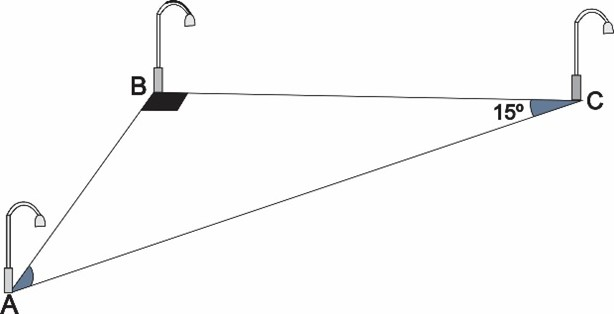
\includegraphics[width=4.5cm]{imagenes/propuestos/geo3.png}
	\end{center}
	
	\begin{enumerate}[label=\Alph*)]
		\item 7 cm
		\item 8 cm
		\item 4 cm
		\item 5 cm
		\item 6 cm
	\end{enumerate}
	
	\item Un paralelogramo $ABCD$, $AB=3$, $BC=5$, $AC=7$. Calcule $m\angle A$.
	\begin{enumerate}[label=\Alph*)]
		\item $120^\circ$
		\item $20^\circ$
		\item $10^\circ$
		\item $25^\circ$
		\item $53^\circ$
	\end{enumerate}
	
	\item En un triángulo rectángulo, uno de los ángulos agudos mide $\dfrac{2\pi}{5}$ rad. Determine el otro ángulo agudo en el sistema sexagesimal.
	\begin{enumerate}[label=\Alph*)]
		\item $-62^\circ$
		\item $73^\circ$
		\item $18^\circ$
		\item $45^\circ$
		\item $26^\circ$
	\end{enumerate}
	
	\item En la figura, determina $\tan\theta$.
	
	\begin{center}
		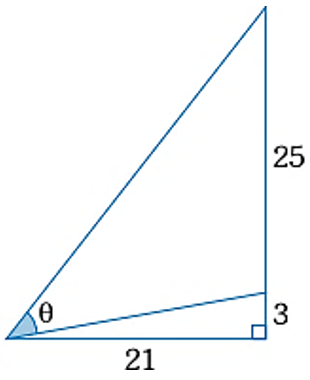
\includegraphics[width=2cm]{imagenes/propuestos/trigo4.png}
	\end{center}
	
	\begin{enumerate}[label=\Alph*)]
		\item $2\sqrt{3}$
		\item 1
		\item 2
		\item 5
		\item 24
	\end{enumerate}
	
	\item Un bloque de 10 kg de masa está sobre el plano inclinado como se muestra en la figura. Determine el tiempo que demora el bloque en llegar a la base del plano. El coeficiente de fricción entre el bloque y el plano es 0,5. $(g=10\ \text{m/s}^2)$
	
	\begin{center}
		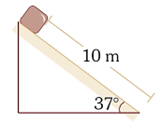
\includegraphics[width=3cm]{imagenes/propuestos/fisica3.png}
	\end{center}
	
	\begin{enumerate}[label=\Alph*)]
		\item $2\sqrt{10}$ s
		\item 4 s
		\item $2\sqrt{5}$ s
		\item $\sqrt{5}$ s
		\item $\sqrt{10}$ s
	\end{enumerate}
	
	\item Qué tiempo debe circular una corriente eléctrica de 10 A por una resistencia de 4,2 $\Omega$ para que con el calor disipado se logre elevar la temperatura de 480 g de agua de $40^\circ$C a $50^\circ$C. $(1\ \text{cal}=4,2\ \text{J})$
	\begin{enumerate}[label=\Alph*)]
		\item 48 s
		\item 480 s
		\item 4,8 s
		\item 12,1 s
		\item 24,0 s
	\end{enumerate}
	
	\item Indica verdadero (V) o falso (F), según corresponda respecto a los isótopos.
	
	I. Son átomos que tienen propiedades químicas idénticas.\\
	II. Son átomos que tienen propiedades físicas diferentes.\\
	III. Todo elemento posee dos o más isótopos naturales, además de ser estables.\\
	IV. Poseen diferente número de nucleones fundamentales.\\
	V. El isótopo más abundante en la naturaleza es el de menor número de masa.
	
	\begin{enumerate}[label=\Alph*)]
		\item FVVFF
		\item VVFVV
		\item FFVFF
		\item FFFVV
		\item VFVVV
	\end{enumerate}
	
	\item Elija tres metales pesados que causan mayor preocupación ecológica.
	\begin{enumerate}[label=\Alph*)]
		\item Hg, As, Li
		\item Pb, Hg, Ag
		\item Hg, Na, Au
		\item Hg, Pb, As
		\item Pb, As, Ag
	\end{enumerate}
	
	\item Entre los músculos de la masticación se encuentra el masetero, cuyo origen es el:
	\begin{enumerate}[label=\Alph*)]
		\item ala mayor de la apófisis pterigoides.
		\item ala menor de la apófisis pterigoides.
		\item borde inferior del hueso parietal.
		\item borde inferior del arco cigomático.
		\item borde inferior de la apófisis pterigoides.
	\end{enumerate}
	
	\item Una de las alternativas corresponde a los trastornos autosómicos dominantes del sistema esquelético.
	\begin{enumerate}[label=\Alph*)]
		\item Neurofibromatosis
		\item distrofia miotónica
		\item síndrome de Marfan
		\item enfermedad de Huntington
		\item borde inferior de la apófisis pterigoides.
	\end{enumerate}
	
	\item Un tema fundamental en la filosofía se refiere al problema relacionado al ser, es decir, determinar qué es primero en la relación ser-pensar. Esta problemática es desarrollada por la rama de la filosofía denominada:
	\begin{enumerate}[label=\Alph*)]
		\item Ontología
		\item Epistemología
		\item Lógica
		\item Idealismo
		\item Metafísica
	\end{enumerate}
	
	\item El saber en general es el conjunto de conocimientos adquiridos por el hombre. El conocimiento científico inicia con el saber:
	\begin{enumerate}[label=\Alph*)]
		\item Espontáneo
		\item Filosófico
		\item Trascendente
		\item Común
		\item Formal
	\end{enumerate}
	
	\item La siguiente descripción: “Se divide en dos sectores, la rama costera y oceánica, transportan entre $40^\circ S$ y $45^\circ S$ masas de agua, son de baja salinidad, alto contenido de oxígeno disuelto, que le permite generar mejores condiciones para la vida marina”; nos referimos a:
	\begin{enumerate}[label=\Alph*)]
		\item La corriente del Niño
		\item La corriente Oceánica
		\item La corriente de Humboldt
		\item La contracorriente del Perú
		\item La corriente Submarina
	\end{enumerate}
	
	\item Las siguientes subcuencas como las de Inambari, Tambopata, Orthon, Las Piedras; pertenecen a la cuenca hidrográfica del río:
	\begin{enumerate}[label=\Alph*)]
		\item Marañón
		\item Ucayali
		\item Madre de Dios
		\item Huallaga
		\item Napo
	\end{enumerate}
	
	\item Las asimetrías entre ricos y pobres en el Perú denotan la forma de violencia denominada:
	\begin{enumerate}[label=\Alph*)]
		\item Estructural
		\item Política
		\item micro social
		\item natural
		\item étnica-cultural
	\end{enumerate}
	
	
		\item Son representantes de la escuela neoliberal.
	
	1. John Keynes\\
	2. Von Hayeck\\
	3. Margaret Thacher\\
	4. Ronald Reagan\\
	5. David Ricardo
	
	Son ciertas:
	\begin{enumerate}[label=\Alph*)]
		\item 1, 2 y 5
		\item 1, 3 y 4
		\item 1, 4 y 5
		\item 3 y 4
		\item 3 y 5
	\end{enumerate}
	
	\item Marque verdad (V) o falsedad (F) en relación con el sistema financiero.
	
	1. Un acreedor financiero es una empresa que obtiene préstamo.\\
	2. La tasa activa y pasiva normalmente son iguales.\\
	3. Una caja rural pertenece al sistema financiero directo.
	
	\begin{enumerate}[label=\Alph*)]
		\item FFF
		\item FVV
		\item VVV
		\item VFF
		\item VVF
	\end{enumerate}
	
	\item Es una característica propia del arcaico superior o de los horticultores sedentarios en la Historia del Perú:
	\begin{enumerate}[label=\Alph*)]
		\item la presencia de la cunicultura
		\item las técnicas de percusión y presión para el tallado de la piedra
		\item la construcción de los primeros centros ceremoniales
		\item la formación de las primeras aldeas
		\item la primera domesticación del perro
	\end{enumerate}
	
	\item Uno de los enunciados no corresponde a la Carta a los Españoles Americanos.
	\begin{enumerate}[label=\Alph*)]
		\item Es un documento de tendencia separatista.
		\item Fue redactado por Juan Pablo Vizcardo y Guzmán.
		\item La versión original fue en francés.
		\item Promueve la idea de patria continental.
		\item Rechaza la presencia de las tropas napoleónicas en España.
	\end{enumerate}
	
	\item El primero en fundamentar que el temor del hombre, por ser antisocial, ha hecho necesario el surgimiento del Estado como autoridad omnipotente e incontrastable, es:
	\begin{enumerate}[label=\Alph*)]
		\item Rousseau
		\item Sócrates
		\item Platón
		\item Hobbes
		\item Aristóteles
	\end{enumerate}
	
	\item En los versos de “Los Reyes Rojos” de Eguren: “Por verde bosque / Y en los purpurinos cerros / Vibra su ceño. // Falcones reyes / Batallan en lejanías / De oro de azulinas // Por la luz cadmio, / Airadas se ven pequeñas, / sus formas negras...”, la influencia de los movimientos literarios son:
	\begin{enumerate}[label=\Alph*)]
		\item sinestesia -- simbolismo
		\item creacionismo -- modernismo
		\item simbolismo -- parnasianismo
		\item pre modernismo -- futurismo
		\item tradicionalismo - esteticismo
	\end{enumerate}
	
	\item El texto: “Aguacero, aguacerito / Granizadita, granizadita / mira, no me mojes / no me granices / tengo manta corta / tengo poncho chico”, corresponde a un:
	\begin{enumerate}[label=\Alph*)]
		\item Aymoray
		\item Coyllur
		\item Arawy
		\item Urpi
		\item Huakatapi
	\end{enumerate}
	
	\item El número de términos que tiene la serie:
	
	$9,\ 12,\ 15,\ 16,\ 21,\ 20,\ \ldots,\ 64$
	
	es:
	
	\begin{enumerate}[label=\Alph*)]
		\item 28
		\item 29
		\item 30
		\item 31
		\item 32
	\end{enumerate}
	
	\item En un examen para ingreso a una Universidad, un postulante comentaba: “De las 80 preguntas formuladas, si hubiera contestado solo la tercera parte de las preguntas que he contestado habría contestado menos de 17 preguntas; además, el triple de las preguntas que no contesté es menor que el doble de preguntas que contesté, disminuido en 5”. La cantidad de preguntas que no contestó el postulante fue:
	\begin{enumerate}[label=\Alph*)]
		\item 10
		\item 30
		\item 50
		\item 52
		\item 54
	\end{enumerate}
	
	\item Elegir la alternativa que contenga el vocablo con el significado antónimo absoluto contextual, respecto del que posee el término subrayado en el enunciado siguiente:
	
	\textit{Es capaz de aglutinar a la gente más dispar.}
	
	\begin{enumerate}[label=\Alph*)]
		\item Unir
		\item Junta
		\item Separar
		\item Extraviar
		\item alentar
	\end{enumerate}
	
	\item Localizar en el texto la idea principal y determinar qué tipo de párrafo es por su ubicación. Texto base:
	
	\textit{Se entiende por libertad a aquella capacidad de autodeterminación de la voluntad, que permite a los seres humanos actuar como deseen. En tal sentido, suele ser denominada libertad individual. El término libertad se vincula a la soberanía de su país en la vertiente de “libertad nacional”. Aunque desde esta perspectiva tradicional, la libertad puede ser civil o política, el concepto moderno incluye un conjunto general de derechos individuales, como la igualdad de oportunidades o el derecho a la educación. Pese a todas estas particularidades históricas se conserva aquella parte esencial de su definición que afirma que libertad es la autonomía de la voluntad a partir de la cual el hombre actúa como mejor le venga en gana.}
	
	\begin{enumerate}[label=\Alph*)]
		\item Encuadrado
		\item Paralelo
		\item Analizante
		\item alternado-centrado
		\item sintetizante
	\end{enumerate}
	
	\item “Yachachiq” simipi, “-q” sufijochasqa ima nirqan?
	\begin{enumerate}[label=\Alph*)]
		\item Mana
		\item Runa
		\item Riqsi
		\item Runapas hina ruwachiq
		\item Tinkuy
	\end{enumerate}
	
	\item ¿Imanallataq “viernes” nisqaqa?
	\begin{enumerate}[label=\Alph*)]
		\item K’anchay
		\item Viernesmanta
		\item Ch’askimanta
		\item Ch’isi
		\item Killachay
	\end{enumerate}
	

	
	\item The boy \_\_\_ won the race is my cousin.
	\begin{enumerate}[label=\Alph*)]
		\item which
		\item where
		\item who
		\item whom
		\item that whom
	\end{enumerate}
	
	\item She usually studies \_\_\_ night.
	\begin{enumerate}[label=\Alph*)]
		\item in
		\item at
		\item on
		\item to
		\item by
	\end{enumerate}
	
	\end{enumerate}




\subsubsection*{Claves de Respuestas}


\begin{center}
	\begin{tabular}{ll ll ll ll ll ll}
		1) E & 2) D & 3) C & 4) C & 5) A & 6) A \\
		7) C & 8) B & 9) E & 10) A & 11) B & 12) D \\
		13) D & 14) C & 15) A & 16) A & 17) C & 18) C \\
		19) A & 20) A & 21) C & 22) E & 23) D & 24) C \\
		25) A & 26) A & 27) B & 28) C & 29) A & 30) D \\
		31) B & 32) C & 33) B & 34) B & & \\
	\end{tabular}
\end{center}


	\thispagestyle{empty}
\addcontentsline{toc}{chapter}{EXAMEN GENERAL 2024-I}
\addcontentsline{toc}{section}{Primera Etapa}

\vspace*{\fill}
\begin{center}
	{\Huge\bfseries EXAMEN GENERAL 2024-I}\\[10pt]
	{\Large\bfseries Primera Etapa}
\end{center}
\vspace*{\fill}

\clearpage




\section*{Área: Ingenierías}


\subsection*{Aritmética}

\begin{enumerate}
	
	
	\item Si: 
	$A = \{ a \in \mathbb{Z} / a^5 - 5a^3 + 4a = 0 \}$ \\
	$B = \{ a \in A / \exists \, b \in \mathbb{Z}, a = b^2 \}$ \\
	Halle la suma de los elementos de $A - B$.
	
	\begin{enumerate}[label=\alph*)]
	\item 0
	\item 1
	\item -1
	\item -2
	\item 2
	\end{enumerate}
	
	\textbf{Respuesta correcta:} a)
	
	\vspace{2mm}
	\textbf{Solucionario:}\\[1mm]
	Con $A$: 
	\begin{align*}
		a^5 - 5a^3 + 4a = 0 &\Rightarrow a(a^4 - 5a^2 + 4) = 0 \\
		&\Rightarrow a(a^2 - 1)(a^2 - 4) = 0 \\
		&\Rightarrow a(a-1)(a+1)(a-2)(a+2) = 0
	\end{align*}
	Entonces: $A = \{ -2; -1; 0; 1; 2 \}$
	
	Con $B$: Para $a = -2 \vee a = -1$, no existe un $b \in \mathbb{Z} / a = b^2$. \\
	$a = 0 \Rightarrow \exists \, b \in \mathbb{Z} / 0 = b^2 \rightarrow b = 0$ \\
	$a = 1 \Rightarrow \exists \, b \in \mathbb{Z} / 1 = b^2 \rightarrow b = -1, 1$ \\
	$a = 2 \Rightarrow \nexists \, b \in \mathbb{Z} / 2 = b^2$
	
	Entonces: $B = \{ 0; 1; -1 \}$
	
	Luego: $A - B = \{ -2; 2 \}$
	
	Piden la suma de sus elementos de $A - B$: $-2 + 2 $\fbox{$= 0$}
	
	
	\vspace{6mm}
	

	\item Hallar el número de seis cifras cuya primera cifra a la izquierda es uno y tal que si esta cifra se traslada a la derecha de la cifra de las unidades, el número así formado es el triple del original.
	
	\begin{enumerate}[label=\alph*)]
		\item $181534$
		\item $121337$
		\item $112857$
		\item $142857$
		\item $135682$
	\end{enumerate}
	
	\textbf{Respuesta correcta:} d)
	
	\vspace{2mm}
	\textbf{Solucionario:}\\[1mm]
	Sea el número: $\overline{1abcde}$ \\
	Dato: $\overline{abcde1} = 3(\overline{1abcde})$
	
	Descomponiendo resulta:
	\begin{align*}
		10(\overline{abcde}) + 1 &= 3(10^5 + \overline{abcde}) \\
		10(\overline{abcde}) + 1 &= 300\,000 + 3(\overline{abcde}) \\
		7(\overline{abcde}) &= 300000 - 1 \\
		7(\overline{abcde}) &= 299999 \\
		\overline{abcde} &= 42857
	\end{align*}
	
	Piden $\overline{1abcde} $ \fbox{$= 142857$}
	
	\vspace{6mm}
	
	\item Si $N$ es un número que descompuesto en sus factores primos es igual a $N = 2^5 \cdot 3^4 \cdot x$ y además $N$ es igual a $\dfrac{24}{77}$ de la suma de sus divisores, halle  la suma de digitos de $x$.
	
	\begin{enumerate}[label=\alph*)]
		\item $3$
		\item $2$
		\item $8$
		\item $6$
		\item $10$
	\end{enumerate}
	
	\textbf{Respuesta correcta:} b)
	
	\vspace{2mm}
	\textbf{Solucionario:}\\[1mm]
	Usamos la fórmula para hallar $S.D_{(N)}$ (Suma de Divisores). \\
	Como $N = 2^5 \cdot 3^4 \cdot x^1$, entonces:
	
	$ N = \dfrac{24}{77} \cdot (S.D_{(N)}) $
	
	$N = \dfrac{24}{77} \left[ \left( \dfrac{2^6 - 1}{2 - 1} \right) \left( \dfrac{3^5 - 1}{3 - 1} \right) \left( \dfrac{x^2 - 1}{x - 1} \right) \right] $
	
		$2^5 \cdot 3^4 \cdot x = \dfrac{24}{77} \cdot \dfrac{63}{1} \cdot \dfrac{242}{2} \cdot (x + 1)$ \\
		
		$2^5 \cdot 3^4 \cdot x = 2^3 \cdot 3^3 \cdot 11 \cdot (x + 1)$ \\
		$2^2 \cdot 3 \cdot x = 11x + 11 $\\
		$12x = 11x + 11 \Rightarrow x = 11$

	
	Suma de cifras de $x$: $1 + 1 $\fbox{$= 2$}
	
	\vspace{6mm}
	
	
	
	\item Se tiene la siguiente distribución de frecuencias respecto al ingreso familiar de 200 familias.
	
	\begin{center}
		\begin{tabular}{|c|c|c|}
			\hline
			Ingreso & $f_i$ & $F_i$ \\ \hline
			$[ \quad ; \quad \rangle$ & 35 & \\ \hline
			$[ \quad ; 240 \rangle$ & & \\ \hline
			$[ \quad ; \quad \rangle$ & 45 & 120 \\ \hline
			$[ \quad ; \quad \rangle$ & & 157 \\ \hline
			$[ 280; \quad \rangle$ & & \\ \hline
			$[ \quad ; \quad ]$ & 20 & \\ \hline
		\end{tabular}
	\end{center}
	
	¿Cuántas familias tienen un ingreso entre S/. 230 y S/. 300?
	
	\begin{enumerate}[label=\alph*)]
		\item 125
		\item 120
		\item 68
		\item 124
		\item 86
	\end{enumerate}
	
	\textbf{Respuesta correcta:} a)
	
	\vspace{2mm}
	\textbf{Solucionario:}\\[1mm]
	Calculamos el ancho de clase ($w$):
	
	% Representación del gráfico de intervalos
	\begin{center}
		\setlength{\unitlength}{1mm}
		\begin{picture}(80,10)
			\put(0,5){\line(1,0){70}}
			\put(0,5){\circle*{1.5}} \put(14,5){\circle*{1.5}} \put(28,5){\circle*{1.5}} 
			\put(42,5){\circle*{1.5}} \put(56,5){\circle*{1.5}} \put(70,5){\circle*{1.5}}
			\put(6,7){\small $w=20$} \put(20,7){\small $w=20$} \put(34,7){\small $w=20$} \put(48,7){\small $w=20$} \put(62,7){\small $w=20$}
			\put(26,1){\small 240} \put(54,1){\small 280}
		\end{picture}
	\end{center}
	
	Se observa: $2w = 40 \Rightarrow w = 20$.
	
	Luego, distribuimos las frecuencias en los intervalos:
	\begin{itemize}
		\item $[200; 220\rangle \rightarrow f_1 = 35$
		\item $[220; 240\rangle \rightarrow f_2 = 120 - 35 - 45 = 40$
		\item $[240; 260\rangle \rightarrow f_3 = 45$
		\item $[260; 280\rangle \rightarrow f_4 = 157 - 120 = 37$
		\item $[280; 300\rangle \rightarrow f_5 = 200 - 157 - 20 = 23$
		\item $[300; 320] \rightarrow f_6 = 20$
	\end{itemize}
	
	Para el rango entre S/. 230 y S/. 300:
	\begin{itemize}
		\item Del intervalo $[220; 240\rangle$, tomamos la mitad (de 230 a 240): $40 / 2 = 20$ familias.
		\item Del intervalo $[240; 260\rangle$: 45 familias.
		\item Del intervalo $[260; 280\rangle$: 37 familias.
		\item Del intervalo $[280; 300\rangle$: 23 familias.
	\end{itemize}
	
	Suma total: $20 + 45 + 37 + 23 $\fbox{$ = 125$}.
	
	Por lo tanto, hay 125 familias que tienen ingresos entre S/. 230 y S/. 300.
	
	

	
	\vspace{6mm}

\end{enumerate}




\subsection*{Álgebra}


\begin{enumerate}[resume]
	
	
	\item Sabiendo que $f(x) = 6x + k$ y $g(x) = 4x - k$, halle el valor de $k$ si se cumple $(f \circ g)(x) + 4 = (g \circ f)(x) - (f - g)(k)$.
	
	\begin{enumerate}[label=\alph*)]
		\item 1
		\item -1
		\item 2
		\item -2
		\item 0
	\end{enumerate}
	
	\textbf{Respuesta correcta:} a)
	
	\vspace{2mm}
	\textbf{Solucionario:}\\[1mm]
	Calculamos las composiciones y la resta:
	\begin{itemize}
		\item $(f \circ g)(x) = f(4x - k) = 6(4x - k) + k = 24x - 5k$
		\item $(g \circ f)(x) = g(6x + k) = 4(6x + k) - k = 24x + 3k$
		\item $(f - g)(k) = f(k) - g(k) = (6k + k) - (4k - k) = 7k - 3k = 4k$
	\end{itemize}
	Reemplazamos en la ecuación original:
	\begin{align*}
		(24x - 5k) + 4 &= (24x + 3k) - 4k \\
		24x - 5k + 4 &= 24x - k \\
		-4k + 4 &= 0 \\
		4 &= 4k \Rightarrow \fbox{k = 1}
	\end{align*}
	
	
	
	
	
	\vspace{6mm}
	
	
	
	
	\item Sean $A$ y $B$ matrices cuadradas del mismo orden. Establezca el valor de verdad de las siguientes proposiciones:
	\begin{enumerate}[label=\Roman*.]
		\item $(A + B)^2 = A^2 + 2AB + B^2$
		\item $|A + B| = |B + A|$
		\item $|A \cdot B| = |A| |B|$
		\item $|A \cdot B^{-1}| =\displaystyle \dfrac{|A|}{|B|}, \text{ donde } |B| \neq 0$
	\end{enumerate}
	
	\begin{enumerate}[label=\alph*)]
		\item FVVV
		\item VFVV
		\item VVVF
		\item VVFF
		\item FFVF
	\end{enumerate}
	
	\textbf{Respuesta correcta:} a)
	
	\vspace{2mm}
	\textbf{Solucionario:}\\[1mm]
	\begin{itemize}
		\item \textbf{I. (F)} Pues $(A + B)^2 = A^2 + AB + BA + B^2$. 
		\item \textbf{II. (V)} La suma de matrices es conmutativa, 
		\item \textbf{III. (V)} Propiedad de los determinantes: el determinante del producto es el producto de los determinantes.
		\item \textbf{IV. (V)} Propiedad de los determinantes: $|B^{-1}| = \displaystyle\dfrac{1}{|B|}$.
	\end{itemize}
	
	
	
	\vspace{6mm}
	
	
	\item Al descomponer $\displaystyle\dfrac{x+1}{(x-1)^3}$ en una suma de fracciones parciales, se encontró que uno de sus sumandos es $\displaystyle\dfrac{A_2}{(x-1)^2}$. ¿Cuál es el valor de $A_2$?
	
	\begin{enumerate}[label=\alph*)]
		\item 1
		\item -1
		\item 2
		\item -2
		\item 3
	\end{enumerate}
	
	\textbf{Respuesta correcta:} a)
	
	\vspace{2mm}
	\textbf{Solucionario:}\\[1mm]
	Planteamos la descomposición:
	\[ \dfrac{x+1}{(x-1)^3} = \dfrac{A_1}{(x-1)} + \dfrac{A_2}{(x-1)^2} + \dfrac{A_3}{(x-1)^3} \]
	Multiplicando todo por $(x-1)^3$:
	\[ x + 1 = A_1(x-1)^2 + A_2(x-1) + A_3 \]
	\[ x + 1 = A_1(x^2 - 2x + 1) + A_2x - A_2 + A_3 \]
	
	Comparando coeficientes:
	\begin{itemize}
		\item Para $x^2$: $A_1 = 0$
		\item Para $x$: $A_2 - 2A_1 = 1 \Rightarrow A_2 - 0 = 1 \Rightarrow A_2 = 1$
		\item Término independiente: $A_1 - A_2 + A_3 = 1 \Rightarrow 0 - 1 + A_3 = 1 \Rightarrow A_3 = 2$
	\end{itemize}
	Por lo tanto, \fbox{$A_2 = 1$}.
	
	
	
	
	\item Halle el volumen máximo de un cilindro, cuya área total es igual a $S$.
	
	\begin{enumerate}[label=\alph*)]
		\item $\displaystyle\dfrac{\pi s^{\dfrac{3}{2}}}{2}$
		\item $\pi$
		\item $\displaystyle\dfrac{s^{\dfrac{3}{2}}}{3\sqrt{6\pi}}$
		\item $\displaystyle\dfrac{\pi}{2} S^3$
		\item $\pi S^{\dfrac{3}{2}}$
	\end{enumerate}
	
	\textbf{Respuesta correcta:} a)
	
	\vspace{2mm}
	\textbf{Solucionario:}\\[1mm]
	$V = \pi r^2 h$ y $S = 2\pi r^2 + 2\pi r h$ \\
	
	Despejamos $h$: $h = \dfrac{S - 2\pi r^2}{2\pi r}$ \\
	
	Luego reemplazamos en $V$:
	
	$V = \pi r^2 \left( \dfrac{S - 2\pi r^2}{2\pi r} \right) = \dfrac{r}{2}(S - 2\pi r^2) = \dfrac{rS}{2} - \pi r^3 $\\
	
	Derivamos para maximizar:\\
	$V' = \dfrac{S}{2} - 3\pi r^2 = 0 \Rightarrow r^2 = \dfrac{S}{6\pi} \Rightarrow r = \sqrt{\dfrac{S}{6\pi}}\\ $
	 $V'' = -6\pi r < 0$ (es un máximo). \\
	 $V = \dfrac{rS}{2} - \dfrac{rS}{6} = \dfrac{rS}{3}\\$ 
	\fbox{$V = \displaystyle\dfrac{s^{\dfrac{3}{2}}}{3\sqrt{6\pi}}$} \\
	
	
	\vspace{6mm}
	
\end{enumerate}


\subsection*{Geometría}

\begin{enumerate}[resume]
	
	\item En la figura, P=(6$\sqrt{3};8$). Halle la distancia del baricentro de la región triángular UNO al punto P.
	
	
	\begin{center}
		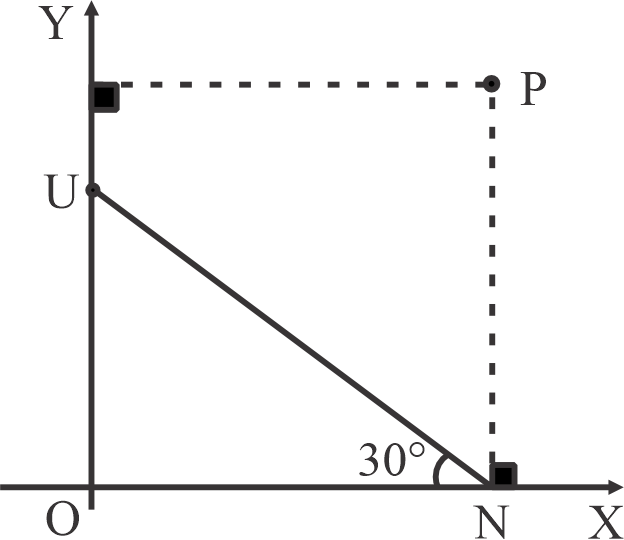
\includegraphics[width=3.5cm]{imagenes/general2024-I/etapa1/ing/geo1g24-I.png}
	\end{center}
	
	\begin{enumerate}[label=\alph*)]
		\item 21
		\item $\sqrt{21}$
		\item $2\sqrt{21}$
		\item $4\sqrt{21}$
		\item $2\sqrt{42}$
	\end{enumerate}
	
	\textbf{Respuesta correcta:} c)
	
	\vspace{2mm}
	\textbf{Solucionario:}\\[1mm]
		
		
	\begin{center}
		\begin{minipage}{0.45\textwidth}
			De la figura:\\
			$x=\dfrac{0+0+6\sqrt{3}}{3}=2\sqrt{3}$\\
			
			$y=\dfrac{0+6+0}{3}=2$\\
			
			$G=(2\sqrt{3},2)$\\
			$d(G,p)=\sqrt{(6\sqrt{3}-2\sqrt{3})^2+(8-2)^2}$\\
			$=\sqrt{16(3)+36}$\\
			$=\sqrt{84}$\\
			\fbox{$=2\sqrt{21}$}
			\vspace{6mm}
		\end{minipage}
		\hfill
		\begin{minipage}{0.45\textwidth}
			\centering
			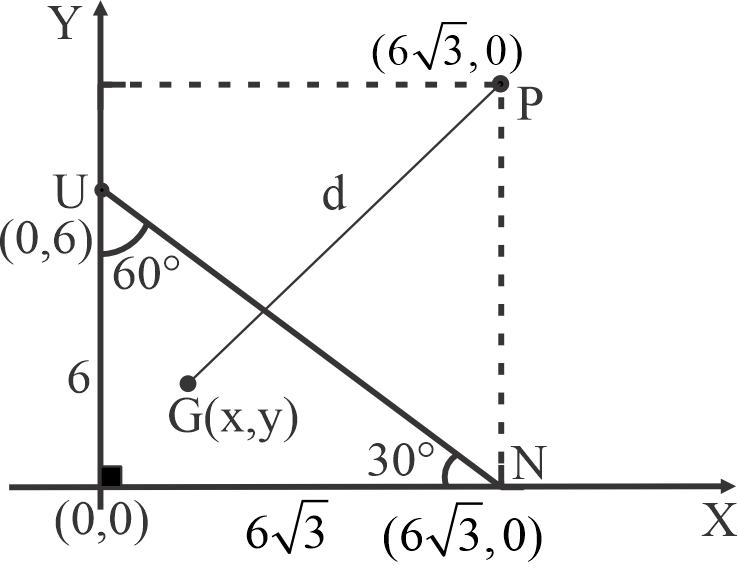
\includegraphics[width=4.5cm]{imagenes/general2024-I/etapa1/ing/geo1g24r-I.png}
		\end{minipage}
	\end{center}
	

	
		\vspace{6mm}
	
	
	
	
	
	\item En un hexágono regular ABCDEF,cuyo apotema mide $3\sqrt{3}$, calcule la medida del apotema del triángulo ACE.
	\begin{enumerate}[label=\alph*)]
		\item 3
		\item 4
		\item 6
		\item 3$\sqrt{2}$
		\item $3\sqrt{3}$
	\end{enumerate}
	
	\textbf{Respuesta correcta:} a)
	
	\vspace{2mm}
	\textbf{Solucionario:}\\[1mm]
	\begin{center}
		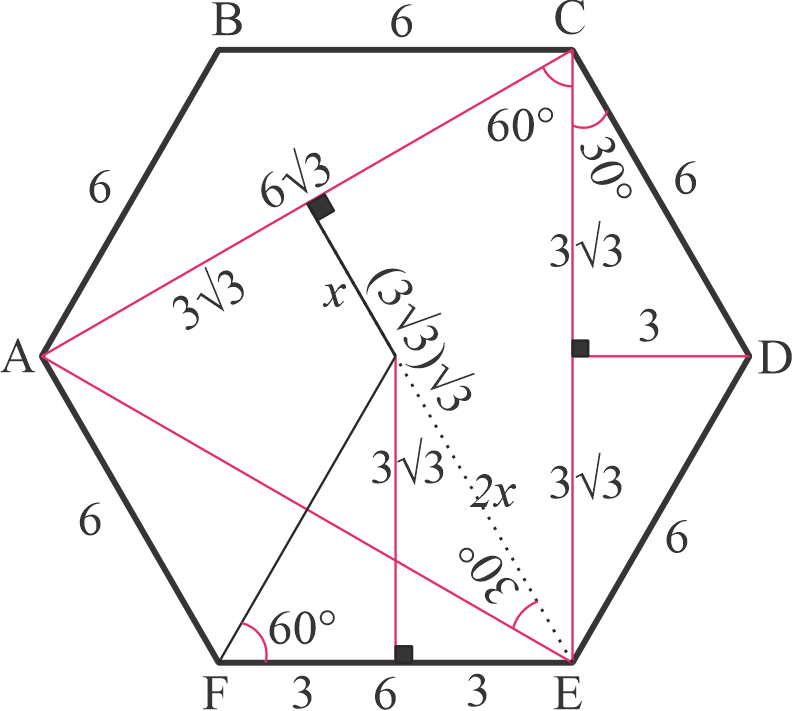
\includegraphics[width=4cm]{imagenes/general2024-I/etapa1/ing/geo2g24-I.png}
	\end{center}
	
	
	
	De la figura se tiene: $3x=9 \Rightarrow $\fbox{$x=3$}
	
	\vspace{6mm}
	
		\item En la figura, si $\alpha + \beta = 130^\circ$, calcule $x + y + z + w + v$.
		
		\begin{center}
			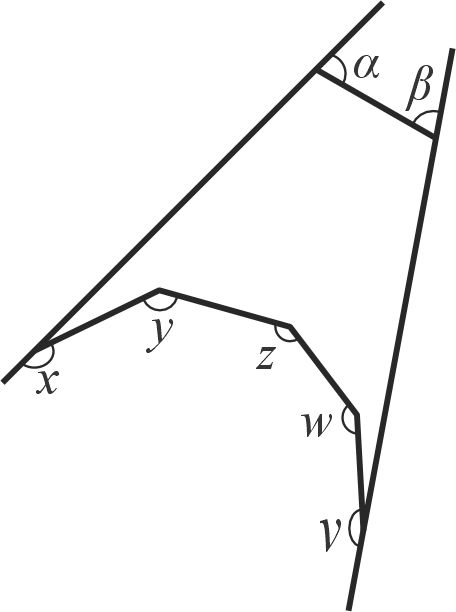
\includegraphics[width=3cm]{imagenes/general2024-I/etapa1/ing/geo3g24-I.png}
		\end{center}
		
	\begin{enumerate}[label=\alph*)]
		\item 920°
		\item 630°
		\item 860°
		\item 770°
		\item 550°
	\end{enumerate}
	
	\textbf{Respuesta correcta:} d)
	
	\vspace{2mm}
	\textbf{Solucionario:}\\[1mm]
	
	
	
		\begin{center}
		\begin{minipage}{0.45\textwidth}
		Del gráfico:\\
		$ \alpha +\beta+ a=180° \rightarrow a=50\\
		m+n+a=180° \rightarrow  m+n=130°\\
		x+y+z+w+v+m+n=180(7-2)\\
		x+y+z+w+v=180°(5)-130°\\
		x+y+z+w+v=900°-130°\\
		$\fbox{$x+y+z+w+v=770°$}
			\vspace{6mm}
		\end{minipage}
		\hfill
		\begin{minipage}{0.45\textwidth}
			\centering
			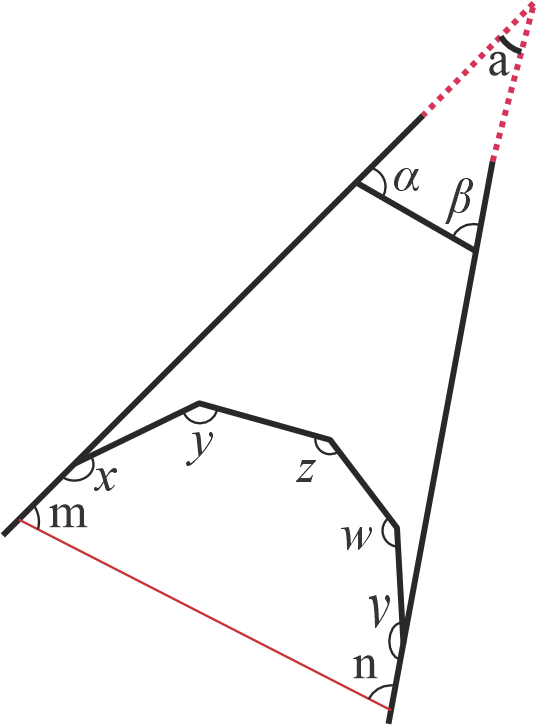
\includegraphics[width=3cm]{imagenes/general2024-I/etapa1/ing/geo3g24r-I.png}
		\end{minipage}
	\end{center}
	
	
	
	\vspace{6mm}
	
		\item Calcule el radio de la circunferencia inscrita en un trapecio rectángulo cuyas bases miden 2 y 3.
	\begin{enumerate}[label=\alph*)]
		\item $\dfrac{3}{5}$
		\item $\dfrac{6}{5}$
		\item $\dfrac{4}{3}$
		\item $\dfrac{2}{3}$
		\item $\dfrac{3}{2}$
	\end{enumerate}
	
	\textbf{Respuesta correcta:} b)
	
	\vspace{2mm}
	\textbf{Solucionario:}\\[1mm]
	\begin{center}
		\begin{minipage}{0.45\textwidth}
			Por relaciones métricas\\
			$ r^2=(2-r)(3-r)\\
			r^2=6-5r+r^2\\
			5r=6$\\
			\fbox{$4r=\dfrac{6}{5}$}
			\vspace{6mm}
		\end{minipage}
		\hfill
		\begin{minipage}{0.45\textwidth}
			\centering
			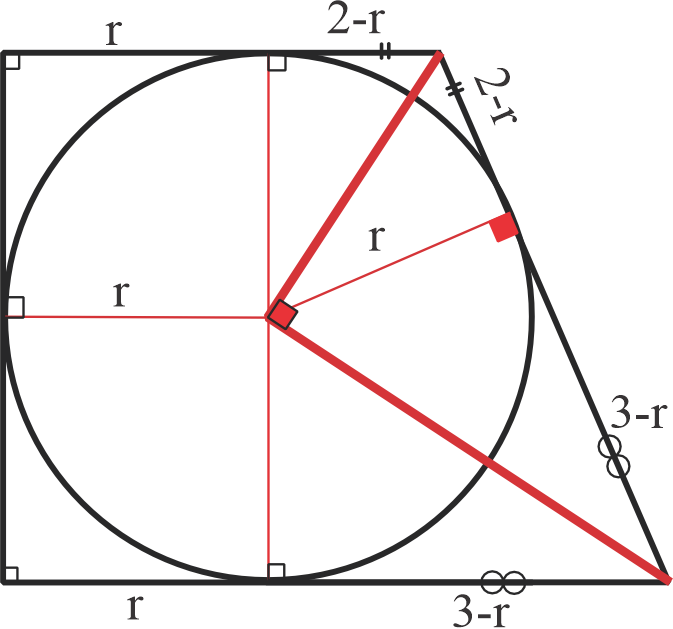
\includegraphics[width=3.8cm]{imagenes/general2024-I/etapa1/ing/geometria4g24-I.png}
		\end{minipage}
	\end{center}
	
	\vspace{6mm}
	
\end{enumerate}



\subsection*{Trigonometría}

\begin{enumerate}[resume]
	
	\item En la figura, halle $\cos 2x$
		
	\begin{center}
		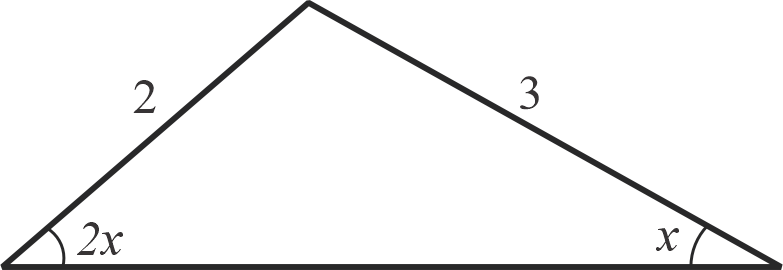
\includegraphics[width=4.5cm]{imagenes/general2024-I/etapa1/ing/trigonometria1g24-I.png}
	\end{center}
	
	\begin{enumerate}[label=\alph*)]
		\item $\displaystyle\dfrac{4}{7}$
		\item $\displaystyle\dfrac{1}{8}$
		\item $\displaystyle\dfrac{7}{8}$
		\item $\displaystyle\dfrac{\sqrt{7}}{2}$
		\item $\displaystyle\dfrac{3}{4}$
	\end{enumerate}
	
	\textbf{Respuesta correcta:} b)
	
	\vspace{2mm}
	\textbf{Solucionario:}\\[1mm]
	
	$\displaystyle\dfrac{\sen 2x}{\sen x}=\displaystyle\dfrac{3}{2}$
	
	$2 \cos x=\dfrac{3}{2}$
		
	$\cos x=\displaystyle\dfrac{3}{4}$
	
	$\cos 2x=2\cos^2x-1$
	
	$\cos 2x=2(\dfrac{3}{4})^2-1$
	
	$\cos2x=\displaystyle\dfrac{9}{8}-1$
	
	\fbox{$\cos2x=\displaystyle\dfrac{1}{8}$}
	
	\vspace{6mm}
	
	\item Halle el valor de 
	\[ M = \tan 35^\circ + \tan 25^\circ + \sqrt{3} \tan 35^\circ \cdot \tan 25^\circ \]
	
	\begin{enumerate}[label=\alph*)]
		\item1
		\item $\dfrac{1}{2}$
		\item $\dfrac{\sqrt{2}}{2}$
		\item $\dfrac{\sqrt{3}}{3}$
		\item $\sqrt{3}$
	\end{enumerate}
	
	\textbf{Respuesta correcta:} b)
	
	\vspace{2mm}
	\textbf{Solucionario:}\\[1mm]
	
	$\tan 60^\circ = \tan(35^\circ + 25^\circ) = \dfrac{\tan 35^\circ + \tan 25^\circ}{1 - \tan 35^\circ \tan 25^\circ}$ \\
	
	$\sqrt{3} = \dfrac{\tan 35^\circ + \tan 25^\circ}{1 - \tan 35^\circ \tan 25^\circ}$ \\
	
	$\sqrt{3} - \sqrt{3} \tan 35^\circ \cdot \tan 25^\circ = \tan 35^\circ + \tan 25^\circ$ \\
	$\sqrt{3} = \tan 35^\circ + \tan 25^\circ + \sqrt{3} \tan 35^\circ \cdot \tan 25^\circ$


	\vspace{6mm}
	
	\item En la figura, determine $\tan\theta + \tan \alpha$.
	
	\begin{center}
		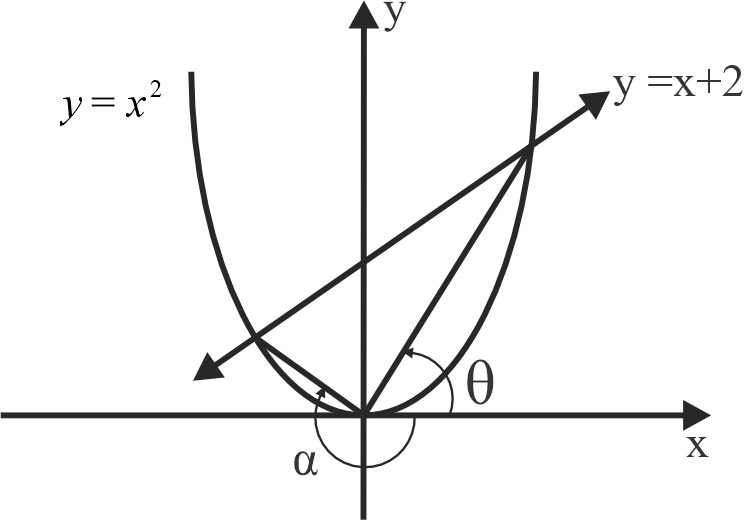
\includegraphics[width=4.3cm]{imagenes/general2024-I/etapa1/ing/trigonometria3g24-I.png}
	\end{center}
	
	
	\begin{enumerate}[label=\alph*)]
		\item 1
		\item -1
		\item 2
		\item -2
		\item -3
	\end{enumerate}
	
	\textbf{Respuesta correcta:} a)
	
	\vspace{2mm}
	\textbf{Solucionario:}\\[1mm]
	
	\begin{center}
		\begin{minipage}{0.45\textwidth}
		$y = x^2 = x + 2$ \\
		$x^2 - x - 2 = 0$ \\
		$(x - 2)(x + 1) = 0$ \\
		$x = 2 \quad x = -1$ \\
		$B(2; 4) \quad \wedge \quad A(-1; 1)$ \\
		$\tan \theta + \tan \alpha$ \\
		$= \dfrac{4}{2} + \dfrac{1}{-1}$ \\
		$= 2 - 1 = 1$
			\vspace{6mm}
		\end{minipage}
		\hfill
		\begin{minipage}{0.45\textwidth}
			\centering
			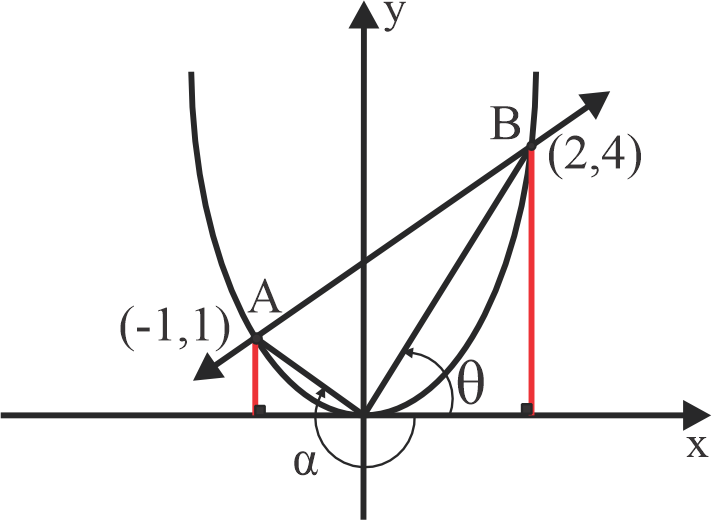
\includegraphics[width=4.3cm]{imagenes/general2024-I/etapa1/ing/trigonometria3g24r-I.png}
		\end{minipage}
	\end{center}
	
	\vspace{6mm}
	
	\item Determine el periodo de la función:\\
	$ g(x) = |\cos^4 x - \sin^4 x| $
	\begin{enumerate}[label=\alph*)]
		\item $\dfrac{\pi}{4}$
		\item $\dfrac{\pi}{2}$
		\item $\dfrac{\pi}{8}$
		\item $\dfrac{\pi}{16}$
		\item $\dfrac{3\pi}{8}$
	\end{enumerate}
	
	\textbf{Respuesta correcta:} b)
	
	\vspace{2mm}
	\textbf{Solucionario:}\\[1mm]
	
	
	\begin{center}
		\begin{minipage}{0.45\textwidth}
		$g(x) = |(\cos^2 x - \sin^2 x)(\underbrace{\cos^2 x + \sin^2 x}_{1})|$ \\
		$g(x) = |\cos^2 x - \sin^2 x|$ \\
		$g(x) = |\cos 2x|$

			\vspace{6mm}
		\end{minipage}
		\hfill
		\begin{minipage}{0.45\textwidth}
			\centering
			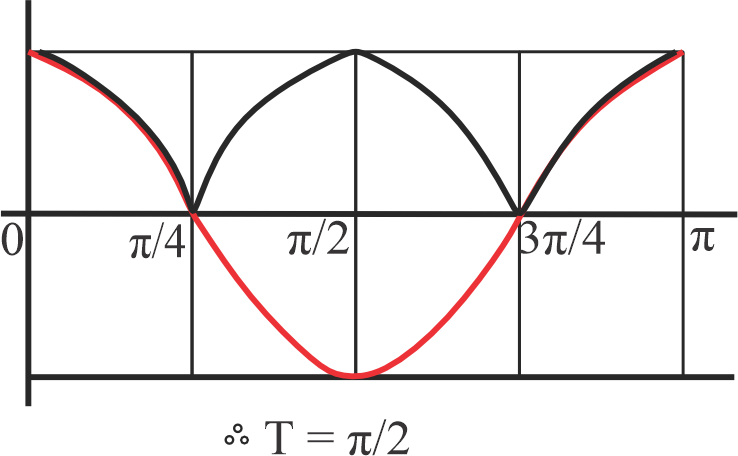
\includegraphics[width=5cm]{imagenes/general2024-I/etapa1/ing/trigonometria4g24-I.png}
		\end{minipage}
	\end{center}
	\vspace{6mm}
	
\end{enumerate}







\subsection*{Física}

\begin{enumerate}[resume]
	
	\item  Un conductor de $1 \Omega$ de resistencia se conecta a una fuente cuyo voltaje varía con el tiempo de acuerdo a la función $\varepsilon = (14 + 2t)V$, donde $t$ está en segundos. ¿Qué cantidad de carga pasa por el conductor en los 3 primeros segundos?

	\begin{enumerate}[label=\alph*)]
		\item 51 C
		\item 50 C
		\item 49 C
		\item 48 C
		\item 52 C
	\end{enumerate}
	
	\textbf{Respuesta correcta:} a)
	
	\vspace{2mm}
	\textbf{Solucionario:}\\[1mm]
	
		\begin{center}
		\begin{minipage}{0.45\textwidth}
			$V = i \cdot R \Rightarrow \varepsilon = i \cdot R$ \\
			$(14 + 2t) = i(1)$ \\
			$i = 14 + 2t$ \\
			Si $t = 0s \Rightarrow i(0) = 14 A$ \\
			Si $t = 3s \Rightarrow i(3) = 14 + 2(3) = 20 A$
			$i = \dfrac{q}{t} \rightarrow q = i \cdot t = \left( \dfrac{14 + 20}{2} \right)(3)$ \\
			$q = (17)(3) = 51 C$
			
			\vspace{6mm}
		\end{minipage}
		\hfill
		\begin{minipage}{0.45\textwidth}
			\centering
			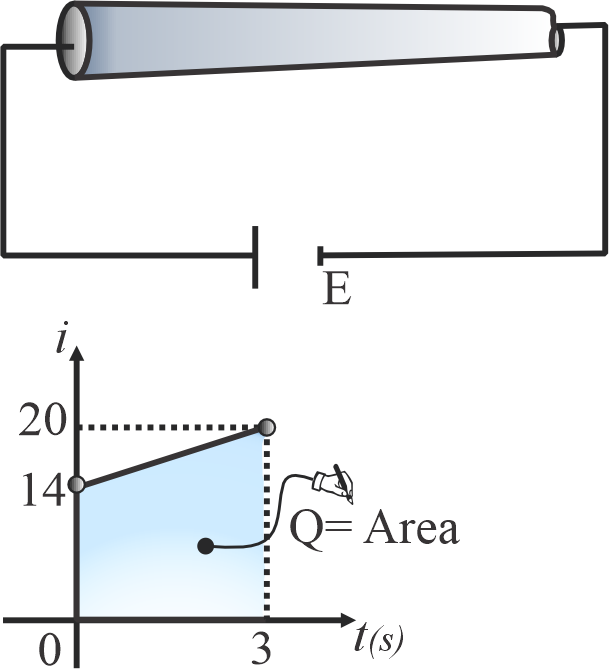
\includegraphics[width=4cm]{imagenes/general2024-I/etapa1/ing/fisica1g24-I .png}
		\end{minipage}
	\end{center}
	\vspace{6mm}
	
	\item Dos esferas de igual Volumen tienen pesos de 10N y 50N respectivamente, se encuentran en el agua flotando unidas mediante un resorte como se muestra en la figura. Halle la deformacion del resorte . (K=5N/cm)
	\begin{center}
		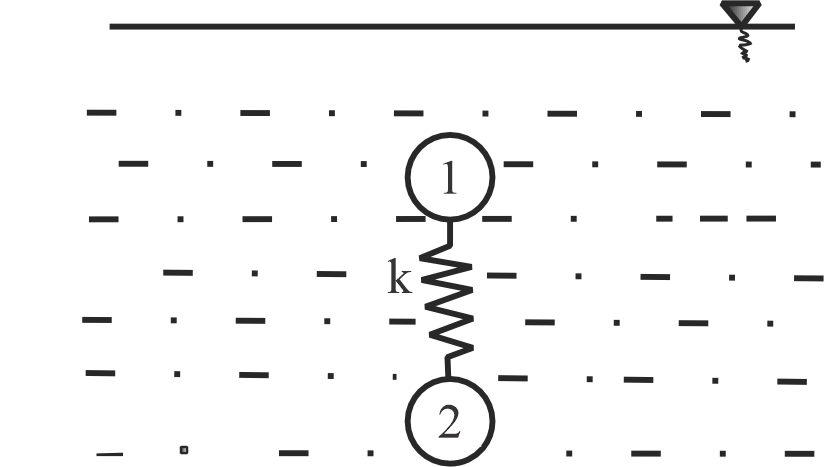
\includegraphics[width=4.5cm]{imagenes/general2024-I/etapa1/ing/fisica2g24-I.png}
	\end{center}
	
	
	\begin{enumerate}[label=\alph*)]
		\item 5 cm
		\item 4 cm
		\item 3 cm
		\item 2 cm
		\item 1 cm
	\end{enumerate}
	
	\textbf{Respuesta correcta:} b)
	
	\vspace{2mm}
	\textbf{Solucionario:}\\[1mm]
	
	\begin{center}
		\begin{minipage}{0.45\textwidth}
			\centering
		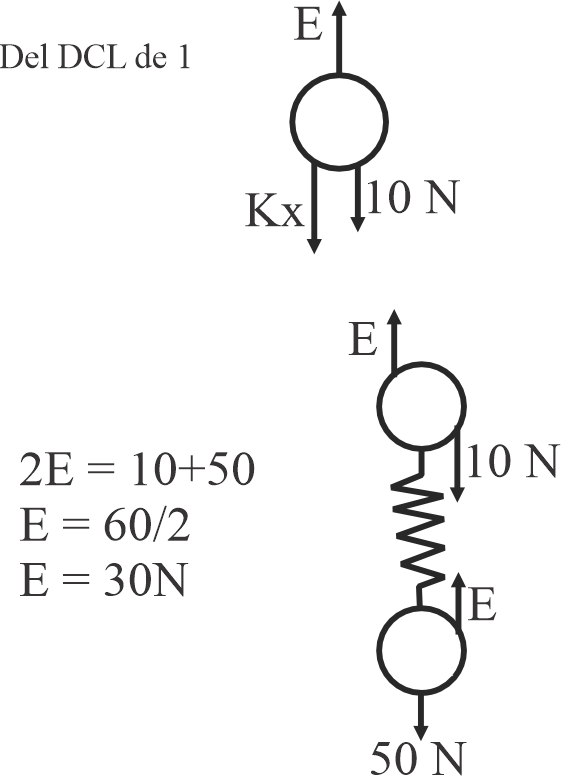
\includegraphics[width=4cm]{imagenes/general2024-I/etapa1/ing/fisica2g24r-I.png}
			
			\vspace{6mm}
		\end{minipage}
		\hfill
		\begin{minipage}{0.45\textwidth}
			$E=Kx+10\\
			x=\dfrac{E-10}{K}.............(*)\\$
			Remplazando E en (*)\\
			$x=\dfrac{30-10(N)}{5N/cm}\\
			x=4cm$\\	
		\end{minipage}
	\end{center}
	
	\vspace{6mm}
	
	
	\item Una hervidora eléctrica de $420 \, W$ se emplea para hacer hervir $1 \, kg$ de agua. Si inicialmente la temperatura del agua es de $10^\circ C$ y el agua hierve a $90^\circ C$, ¿en cuánto tiempo se logra hervir el agua? ($1 \, cal = 4,2 \, J$)
	
	\begin{enumerate}[label=\alph*)]
		\item 820 s
		\item 840 s
		\item 810 s
		\item 800 s
		\item 799 s
	\end{enumerate}
	
	\textbf{Respuesta correcta:} d)
	
	\vspace{2mm}
	\textbf{Solucionario:}\\[1mm]
	$Q = C_e \cdot m \cdot \Delta T$ \\
	$Q = \left( 1 \, \dfrac{cal}{g \cdot ^\circ C} \right) (1000 \, g) (90 - 10) \, ^\circ C$ \\
	$Q = 80 \times 10^3 \, cal$ \\
	$Q = 8 \times 10^4 \times 4,2 \, J$ \\
	$Q = 33,6 \times 10^4 \, J$ \\
	$Q = 336 \, kJ$ \\
	
	$P = \dfrac{Q}{t} \Rightarrow t = \dfrac{Q}{P} = \dfrac{336 \, kJ}{420 \, W}$ \\
	$t = \dfrac{8 \times 10^3 \times 4,2 \times 10}{420} = 800 \, s$

	\vspace{6mm}


\item Si la longitud de un péndulo simple se incrementaría en $4 \, m$, su periodo se quintuplicaría. ¿Cuál es la longitud de dicho péndulo?

\begin{enumerate}[label=\alph*)]
	\item $1/6 \, m$
	\item $1/4 \, m$
	\item $1/5 \, m$
	\item $1/3 \, m$
	\item $1/2 \, m$
\end{enumerate}

\textbf{Respuesta correcta:} a)

\vspace{2mm}
\textbf{Solucionario:}\\[1mm]
$T = 2\pi \sqrt{\dfrac{\ell}{g}}$ \\
$5T = 2\pi \sqrt{\dfrac{\ell + 4}{g}}$ \\

Dividiendo:
$\dfrac{T}{5T} = \dfrac{2\pi \sqrt{\dfrac{\ell}{g}}}{2\pi \sqrt{\dfrac{\ell + 4}{g}}}$ \\

$\left( \dfrac{1}{5} \right)^2 = \left( \sqrt{\dfrac{\dfrac{\ell}{g}}{\dfrac{\ell + 4}{g}}} \right)^2 = \left( \sqrt{\dfrac{\ell}{\ell + 4}} \right)^2$ \\

$\dfrac{1}{25} = \dfrac{\ell}{\ell + 4} \Rightarrow \ell + 4 = 25\ell$ \\

$4 = 24\ell$ \\

$\ell = \dfrac{4}{24} = \dfrac{1}{6} \, m$

\vspace{6mm}
\end{enumerate}



\subsection*{Química}

\begin{enumerate}[resume]
	
	
	
	
	
	\item Calcule el porcentaje de pureza de un mineral de $Fe$, si una muestra de $500 gramos$ del mineral impuro produce $12 gramos$ de hidrógeno según la siguiente reacción:
	
	$Fe_{(s)} + HCl_{(ac)} \longrightarrow FeCl_3 + H_{2(g)}$
	
	$(Fe = 56; \quad H = 1; \quad Cl = 35.5)$
	
	\begin{enumerate}[label=\alph*)]
		\item 46.4\%
		\item 44.8\%
		\item 43.8\%
		\item 48.4\%
		\item 40.4\%
	\end{enumerate}
	
	\textbf{Respuesta correcta:} b)
	
	\vspace{2mm}
	\textbf{Solucionario:}\\[1mm]
	Primero se debe balancear: \\
	$Fe_{(s)} + 3HCl_{(ac)} \rightarrow FeCl_3 + \dfrac{3}{2}H_{2(g)}$
	
	\vspace{2mm}
	\begin{tabular}{l c l}
		Si $Fe_{(s)}$ & \textemdash $\rightarrow$ & $\dfrac{3}{2} H_{2(g)}$ \\
		
		
		$56$ & \textemdash & $\dfrac{3}{2}(1 \times 2)$ \\
		
		$X_{Fe}$ & \textemdash & $12$ \\
	\end{tabular}
	
	\vspace{2mm}
	$X_{Fe} = 224g$
	
	\vspace{4mm}
	Determinando la pureza: \\
	Pureza $= \dfrac{Masa \: sustancia \: pura \: Fe}{Masa \: del \: mineral \: Fe} \times 100$ \\
	
	Pureza $= \dfrac{224g}{500g} \times 100$ \\
	Pureza $= 44.8\%$
	
	\vspace{6mm}
	
	
	
	\item ¿Qué cantidad de energía en joule se libera cuando se transforma en su totalidad, $5g$ de materia?
	
	\begin{enumerate}[label=\alph*)]
		\item $45 \times 10^{16}$
		\item $4,5 \times 10^{14}$
		\item $45 \times 10^{12}$
		\item $4,5 \times 10^{15}$
		\item $4,5 \times 10^{16}$
	\end{enumerate}
	
	\textbf{Respuesta correcta:} b)
	
	\vspace{2mm}
	\textbf{Solucionario:}\\[1mm]
	\textbf{datos} \\
	$E = ?$ J \\
	$m = 5g$ \\
	$c = 3 \times 10^8 m/s$\\

	$E = mc^2$ \\
	$E = 5 \times 10^{-3} kg * (3 \times 10^8 m/s)^2$ \\
	$E = 5 \times 10^{-3} * 9 \times 10^{16}$ \\
	$E = 45 \times 10^{13} J$ \\
	$E = 4,5 \times 10^{14} J.$
	
	\vspace{6mm}
	
	\item Indique Verdadero (V) o Falso (F) a las siguientes proposiciones, según corresponda:
	
	I. El ácido clorhídrico es uno de los componentes de la lluvia ácida.
	
	II. En una zona urbana debe generarse más lluvia ácida que en una zona rural.
	
	III. Un combustible con alto contenido de azufre es un promotor de la lluvia ácida.
	
	\begin{enumerate}[label=\alph*)]
		\item FFV
		\item VVF
		\item FVV
		\item FVF
		\item VFV
	\end{enumerate}
	
	\textbf{Respuesta correcta:} a)
	
	\vspace{2mm}
	\textbf{Solucionario:}\\[1mm]

	Los componentes de la lluvia ácida son los ácidos azufre y nitrógeno como $H_2SO_4$ (ácido sulfúrico) y $HNO_3$ (ácido nítrico).
	
	Los gases producidos como el $NO_x$ y $SO_x$ causan la lluvia ácida.
	
	\vspace{6mm}
	
	\item Se tiene $150g$ de una disolución que contiene $6\%$ de cierta sal, y se requiere reducir al $5\%$, ¿Qué cantidad de agua se debe añadir?
	
	\begin{enumerate}[label=\alph*)]
		\item 25 g
		\item 30g
		\item 20 g
		\item 35 g
		\item 40 g
	\end{enumerate}
	
	\textbf{Respuesta correcta:} b)
	
	\vspace{2mm}
	\textbf{Solucionario:}\\[1mm]

	DATOS \\
	$m_1 = 150g$ disolución \\
	$C_1 = 6\%$ \\
	$C_2 = 5\%$ \\
	$m_2 = m_1 + x$
	
	\vspace{2mm}
	$\Rightarrow C_1 \cdot M_1 = C_2 \cdot M_2$ \\
	$6\% (150) = 5\% (m_1 + x)$ 
	
	$\dfrac{6}{100} (150) = \dfrac{5}{100} (150 + x)$ 
	
	$900 = 750 + 5x$ \\
	$x = 30g$
	
	\vspace{6mm}
	
\end{enumerate}








\subsection*{Biología y Anatomía}

\begin{enumerate}[resume]

	\item La unidad de conservación que protege en forma intangible una especie o una comunidad determinada de plantas y/o animales, así como las formaciones naturales de interés científico y paisajístico, se denomina:
	
	\begin{enumerate}[label=\alph*)]
		\item Parque nacional.
		\item Reserva nacional.
		\item Santuario histórico.
		\item Reserva comunal.
		\item Santuario nacional.
	\end{enumerate}
	
	\textbf{Respuesta correcta:} e)
	
	\vspace{2mm}
	\textbf{Solucionario:}\\[1mm]
	Los Santuarios Nacionales son áreas de carácter intangible destinadas a proteger especies específicas de la flora y fauna, así como formaciones naturales únicas. A diferencia de los Parques Nacionales que protegen ecosistemas amplios, el Santuario se enfoca en comunidades o especies determinadas.
	
	\vspace{6mm}
	
	\item La fermentación alcohólica en la célula se realiza a nivel de:
	
	\begin{enumerate}[label=\alph*)]
		\item citosol
		\item matriz mitocondrial
		\item membrana externa mitocondrial
		\item cresta mitocondrial
		\item cloroplasto
	\end{enumerate}
	
	\textbf{Respuesta correcta:} a)
	
	\vspace{2mm}
	\textbf{Solucionario:}\\[1mm]
	La fermentación (tanto alcohólica como láctica) es un proceso anaeróbico que ocurre íntegramente en el citosol (citoplasma) de la célula. A diferencia de la respiración celular aeróbica, no requiere de las mitocondrias para la obtención de energía (ATP).
	
	\vspace{6mm}
\end{enumerate}




\subsection*{Psicología y Filosofía}

\begin{enumerate}[resume]
	
	
	\item La profesora utiliza láminas de colores para que los estudiantes puedan prestar atención durante toda la clase. Es una característica de la atención:
	
	\begin{enumerate}[label=\alph*)]
		\item direccional.
		\item selectiva.
		\item distributiva.
		\item constante.
		\item intencional.
	\end{enumerate}
	
	\textbf{Respuesta correcta:} a)
	
	\vspace{2mm}
	\textbf{Solucionario:}\\[1mm]
	La atención direccional se refiere a la capacidad de orientar los recursos sensoriales y cognitivos hacia un estímulo específico que destaca en el entorno (en este caso, las láminas de colores) para facilitar el procesamiento de la información.
	
	\vspace{6mm}
	
	\item Juan Victor desea aprender a bailar por eso práctica semanalmente. Este es un tipo de aprendizaje:
	
	\begin{enumerate}[label=\alph*)]
		\item afectivo.
		\item cognositivo.
		\item motor.
		\item social.
		\item actitudinal.
	\end{enumerate}
	
	\textbf{Respuesta correcta:} c)
	
	\vspace{2mm}
	\textbf{Solucionario:}\\[1mm]
	El aprendizaje motor involucra la adquisición de habilidades que requieren coordinación muscular, destreza física y ejecución de movimientos complejos. La práctica semanal del baile es un ejemplo clásico de cómo se automatizan estas secuencias motoras.
	
	\vspace{6mm}
	
	\item El relato ficticio que intenta explicar un aspecto de la realidad se denomina:
	
	\begin{enumerate}[label=\alph*)]
		\item filosofía.
		\item ciencia.
		\item mito.
		\item metafísica.
		\item poesía.
	\end{enumerate}
	
	\textbf{Respuesta correcta:} c)
	
	\vspace{2mm}
	\textbf{Solucionario:}\\[1mm]
	El mito es una narración tradicional y ficticia, protagonizada a menudo por seres sobrenaturales, que busca dar una explicación simbólica u ontológica a fenómenos de la naturaleza o aspectos de la condición humana antes del surgimiento del pensamiento racional-científico.
	
	\vspace{6mm}
	
	\item Si José es un sismólogo que se encarga de tomar nota de todos los detalles de los movimientos telúricos que azotan al Perú, está cumpliendo con la función ... de la ciencia.
	
	\begin{enumerate}[label=\alph*)]
		\item explicativa
		\item aplicativa
		\item social
		\item descriptiva
		\item predictiva
	\end{enumerate}
	
	\textbf{Respuesta correcta:} d)
	
	\vspace{2mm}
	\textbf{Solucionario:}\\[1mm]
	La función descriptiva de la ciencia consiste en registrar, organizar y detallar las características o propiedades de un objeto o fenómeno de estudio. Al "tomar nota de todos los detalles", el sismólogo está respondiendo a la pregunta "¿cómo es?" el fenómeno observado.
	
	\vspace{6mm}
	
\end{enumerate}



\vspace{6mm}



\subsection*{Geografía}

\begin{enumerate}[resume]
	
\item A la relación que existe entre las dimensiones del terreno y las dimensiones que se registran de ese terreno en un mapa, se denomina:

\begin{enumerate}[label=\alph*)]
	\item Proyección cartográfica
	\item Coordenada geográfica
	\item Curva de nivel
	\item Escala cartográfica
	\item Latitud y longitud
\end{enumerate}

\textbf{Respuesta correcta:} d)

\vspace{2mm}
\textbf{Solucionario:}\\[1mm]
La escala cartográfica es la relación matemática que existe entre las dimensiones reales del territorio y las dimensiones representadas en el mapa. Permite calcular distancias reales a partir de una representación reducida.

\vspace{6mm}

\item El fenómeno que eleva la temperatura de la costa norte y avanza hacia el sur del Perú, se llama:

\begin{enumerate}[label=\alph*)]
	\item Corriente de Humbolt
	\item Anticiclón del Pacífico sur
	\item Corriente de El Niño
	\item Anticiclón del Atlántico sur
	\item Corriente peruana
\end{enumerate}

\textbf{Respuesta correcta:} c)

\vspace{2mm}
\textbf{Solucionario:}\\[1mm]
La Corriente de El Niño consiste en la llegada de masas de agua cálida procedentes del norte hacia las costas peruanas. Este fenómeno provoca un aumento anómalo de la temperatura del mar y del aire en la costa norte, extendiéndose ocasionalmente hacia el sur.

\vspace{6mm}	
	
\end{enumerate}


\subsection*{Historia}

\begin{enumerate}[resume]
	
\item La arquitectura \_\_\_\_\_\_\_\_\_\_\_\_\_\_\_ apareció en el siglo XII y perduró hasta fines del XV, sus principales características fueron la ojiva o bóveda elíptica, el arco quebrado o en punta de lanza, las columnas finas y los vitrales.

\begin{enumerate}[label=\alph*)]
	\item medieval
	\item gótica
	\item románica
	\item renacentista
	\item barroca
\end{enumerate}

\textbf{Respuesta correcta:} b)

\vspace{2mm}
\textbf{Solucionario:}\\[1mm]
La arquitectura gótica es el estilo predominante en la Baja Edad Media. Sus innovaciones técnicas, como el arco apuntado (ojiva) y la bóveda de crucería, permitieron construir edificios mucho más altos y con grandes ventanales adornados con vitrales, diferenciándose del estilo románico, que era más robusto y oscuro.

\vspace{6mm}

\item Tras la renuncia del Ing. Alberto Fujimori, el Dr. Valentín Paniagua ocupa la presidencia del Perú entre el 2000 y 2001. Asumió dicho cargo a partir de su condición de

\begin{enumerate}[label=\alph*)]
	\item congresista de la República.
	\item primer ministro del gobierno.
	\item embajador ante la ONU.
	\item candidato electo.
	\item presidente del Congreso de la República.
\end{enumerate}

\textbf{Respuesta correcta:} e)

\vspace{2mm}
\textbf{Solucionario:}\\[1mm]
Tras la crisis política del año 2000 y la vacancia de la presidencia y las vicepresidencias, la línea de sucesión constitucional estableció que el cargo debía ser asumido por el Presidente del Congreso. Valentín Paniagua, quien ocupaba dicha posición en ese momento, asumió la presidencia de un gobierno de transición para convocar a nuevas elecciones.

\vspace{6mm}	
	
\end{enumerate}




\subsection*{Educación Cívica}

\begin{enumerate}[resume]
	
	\item Según la estructura jerárquica del sistema jurídico normativo del Perú, los decretos supremos, los edictos municipales y los decretos regionales ejecutivos, corresponden al:
	
	\begin{enumerate}[label=\alph*)]
		\item I nivel — constitucional.
		\item II nivel — legal.
		\item III nivel — reglamentario.
		\item IV nivel — resoluciones.
		\item V nivel — normas de interés particular.
	\end{enumerate}
	
	\textbf{Respuesta correcta:} c)
	
	\vspace{2mm}
	\textbf{Solucionario:}\\[1mm]
	En la pirámide de Kelsen aplicada al sistema peruano, el tercer nivel (nivel reglamentario) agrupa normas de carácter administrativo general emitidas por el Ejecutivo y gobiernos locales. Los decretos supremos y edictos municipales reglamentan las leyes de jerarquía superior sin contravenirlas.
	
	\vspace{6mm}
	
	\item Según Karl Loewenstein, bajo el sistema político del constitucionalismo, un tipo de democracia constitucional es:
	
	\begin{enumerate}[label=\alph*)]
		\item el nacional — socialismo alemán.
		\item el comunismo chino.
		\item la democracia popular.
		\item la democracia directa.
		\item el neopresidencialismo.
	\end{enumerate}
	
	\textbf{Respuesta correcta:} d)
	
	\vspace{2mm}
	\textbf{Solucionario:}\\[1mm]
	Karl Loewenstein clasifica los sistemas según el ejercicio del poder. En el marco del constitucionalismo, donde el poder está limitado y controlado, la democracia directa se considera una forma pura de democracia constitucional donde la soberanía reside y es ejercida sin intermediarios por el pueblo dentro de un orden jurídico establecido.
	
	\vspace{6mm}
	
\end{enumerate}


\vspace{6mm}


\subsection*{Economía}

\begin{enumerate}[resume]
	
	\item La toma de decisiones de un productor con el objetivo de maximizar sus beneficios, es campo de estudio de la ...
	
	\begin{enumerate}[label=\alph*)]
		\item macroeconomía.
		\item microeconomía.
		\item política económica.
		\item economía política.
		\item economía normativa.
	\end{enumerate}
	
	\textbf{Respuesta correcta:} b)
	
	\vspace{2mm}
	\textbf{Solucionario:}\\[1mm]
	La microeconomía estudia el comportamiento individual de los agentes económicos, como consumidores y empresas (productores). El análisis de cómo un productor decide niveles de producción y costos para maximizar su utilidad es un tema central de esta rama.
	
	\vspace{6mm}
	
	\item En relación a las exportaciones de la economía Peruana se puede afirmar que se ...
	
	\begin{enumerate}[label=\alph*)]
		\item venden maquinarias y equipos.
		\item concentra en productos no tradicionales.
		\item elaboran productos con mucho valor agregado.
		\item concentra en el oro, el cobre y la harina de pescado.
		\item concentra en productos tradicionales con mucho valor agregado.
	\end{enumerate}
	
	\textbf{Respuesta correcta:} d)
	
	\vspace{2mm}
	\textbf{Solucionario:}\\[1mm]
	La estructura exportadora del Perú es primario-exportadora. Esto significa que la mayor parte de las divisas provienen de productos tradicionales (materias primas con bajo valor agregado), destacando principalmente los minerales como el oro y el cobre, además de la harina de pescado.
	
	\vspace{6mm}
	
\end{enumerate}


\subsection*{Comunicación}

\begin{enumerate}[resume]
	
\item La computadora es la consecuencia de muchos inventos del hombre para hacer más fácil los cálculos matemáticos, la composición de textos, el diseño de gráficos, etc.
En el texto, ¿Qué tipo de coma se utiliza?

\begin{enumerate}[label=\alph*)]
	\item coma elíptica
	\item coma apositiva
	\item coma enfática
	\item coma enumerativa
	\item coma explicativa
\end{enumerate}

\textbf{Respuesta correcta:} d)

\vspace{2mm}
\textbf{Solucionario:}\\[1mm]
La coma enumerativa se utiliza para separar elementos análogos dentro de una serie o lista. En el texto, se emplea para separar las distintas funciones de la computadora: "...cálculos matemáticos, la composición de textos, el diseño de gráficos...".

\vspace{6mm}

\item Los seres vivos que existen en nuestro planeta pueden clasificarse de acuerdo a la forma como obtienen sus alimentos. Según estas características pueden ser autótrofos y heterótrofos.
¿A qué tipo de texto corresponde?

\begin{enumerate}[label=\alph*)]
	\item Descriptivo
	\item Argumentativo
	\item Narrativo
	\item Instructivo
	\item Expositivo
\end{enumerate}

\textbf{Respuesta correcta:} e)

\vspace{2mm}
\textbf{Solucionario:}\\[1mm]
El texto es expositivo porque su intención principal es informar y transmitir datos de manera objetiva sobre un tema específico (la clasificación de los seres vivos según su alimentación), sin intentar convencer al lector ni contar una historia.

\vspace{6mm}

\item El presidente del barrio San José convoca a una reunión extraordinaria y pide a su secretario tomar anotaciones del suceso.
¿Qué documento redactará el secretario?

\begin{enumerate}[label=\alph*)]
	\item Solicitud
	\item Carta
	\item Memorando
	\item Acta
	\item Oficio
\end{enumerate}

\textbf{Respuesta correcta:} d)

\vspace{2mm}
\textbf{Solucionario:}\\[1mm]
El acta es el documento oficial donde se registran de manera detallada los hechos, acuerdos y deliberaciones ocurridos durante una reunión o asamblea. Es la función específica del secretario dar fe de lo sucedido mediante este documento.

\vspace{6mm}

\item En la narración, la parte donde se presenta los personajes y el lugar de los eventos se denomina:

\begin{enumerate}[label=\alph*)]
	\item Título
	\item Inicio
	\item Nudo
	\item Desarrollo
	\item Desenlace
\end{enumerate}

\textbf{Respuesta correcta:} b)

\vspace{2mm}
\textbf{Solucionario:}\\[1mm]
El inicio (o planteamiento) es la parte inicial de una estructura narrativa. Su función es situar al lector en el contexto, presentando a los personajes principales, el tiempo y el lugar donde se desarrollará la acción antes de que aparezca el conflicto.

\vspace{6mm}
	
\end{enumerate}






\subsection*{Literatura}

\begin{enumerate}[resume]
	
	\item Los temas fundamentales que desarrolla Kafka en sus obras son:
	
	\begin{enumerate}[label=\alph*)]
		\item el capitalismo y el abuso.
		\item el caos y el absurdo.
		\item la dominación y el servilismo.
		\item la deshumanización y el amor
		\item el rechazo al mundo y el deshonor
	\end{enumerate}
	
	\textbf{Respuesta correcta:} b)
	
	\vspace{2mm}
	\textbf{Solucionario:}\\[1mm]
	Franz Kafka es el máximo exponente de la literatura del absurdo. Sus obras exploran la angustia existencial del individuo frente a situaciones caóticas, burocráticas e incomprensibles donde la lógica común no aplica, reflejando la desorientación del hombre moderno.
	
	\vspace{6mm}
	
	\item Mariano Melgar, para crear el Yaraví, tuvo como referencia al...
	
	\begin{enumerate}[label=\alph*)]
		\item haylli.
		\item lanka.
		\item haravicu.
		\item huayño
		\item harawi.
	\end{enumerate}
	
	\textbf{Respuesta correcta:} e)
	
	\vspace{2mm}
	\textbf{Solucionario:}\\[1mm]
	El Yaraví melgariano tiene su origen en el \textit{harawi} incaico, una especie lírica de tono melancólico y sentimental que expresaba el dolor por la ausencia o pérdida de la amada. Melgar asimiló esta tradición indígena y la fusionó con formas métricas españolas.
	
	\vspace{6mm}
	
\end{enumerate}







\subsection*{Razonamiento Matemático}

\begin{enumerate}[resume]
	
	\item Se tiene un reloj de agujas que a las 0:00 horas del primero de enero marcaba las 5:50 a.m. Si dicho reloj se adelanta 30 segundos cada hora, ¿Cuántas veces durante el año marcará la hora correcta?
	
	\begin{enumerate}[label=\alph*)]
		\item 4
		\item 8 
		\item 12 
		\item 2
		\item 6
	\end{enumerate}
	
	\textbf{Respuesta correcta:} e)
	
	\vspace{2mm}
	\textbf{Solucionario:}\\[1mm]
	Determinando cada cuántos días marcará la hora correcta:
	
	Para que un reloj de agujas vuelva a marcar la hora correcta, debe acumular un adelanto de 12 horas (720 minutos).
	
	\begin{itemize}
		\item Adelanta: $30s = \dfrac{1}{2}$ min $\xrightarrow{\times 2}$ en 1 h.
		\item Adelanta: 720 min $\xrightarrow{\times 2}$ en 1440 h.
	\end{itemize}
	
	Convertimos las horas a días:
	$1440 \text{ h} = \dfrac{1440}{24} = 60 \text{ días.}$
	
	$\Rightarrow$ Cada 60 días marcará la hora exacta.
	
	\vspace{2mm}
	\textbf{Para un año (365 días):}
	$\# \text{ veces} = \dfrac{365}{60} \approx 6 \text{ veces.}$
	
	\vspace{6mm}

	
	\item Si a cada uno de los 4 términos de una proporción geométrica se le quita una misma cantidad, se obtendrá 20, 28, 32 y 44. Halle la suma de los términos de la proporción.
	
	\begin{enumerate}[label=\alph*)]
		\item 140
		\item 124
		\item 144
		\item 112
		\item 104
	\end{enumerate}
	
	\textbf{Respuesta correcta:} a)
	
	\vspace{2mm}
	\textbf{Solucionario:}\\[1mm]
	La proporción: $\dfrac{a}{b} = \dfrac{c}{d} \quad \text{(I)}$
	
	Se le quita la misma cantidad:
	$\left. \begin{array}{l} 
		a - x = 20 \Rightarrow a = 20 + x \\
		b - x = 28 \Rightarrow b = 28 + x \\
		c - x = 32 \Rightarrow c = 32 + x \\
		d - x = 44 \Rightarrow d = 44 + x 
	\end{array} \right\} \text{(II)}$
	
	Se tendrá que:\\
	$a + b + c + d = 124 + 4x \quad \text{(III)}$
	
	Remplazando (II) en (I) y resolviendo:
	$$\dfrac{20 + x}{28 + x} = \dfrac{32 + x}{44 + x} \Rightarrow 880 + 64x + x^2 = 896 + 60x + x^2$$
	$4x = 16 \Rightarrow x = 4$
	
	Se pide $a + b + c + d = ?$\\
	De (III): $a + b + c + d = 124 + 4(4) = 140$
	
	\vspace{6mm}


\item En un pastizal, una vaca es atada a una estaca con una cuerda de 4 metros. Comiendo la misma cantidad de pasto diario, consumió todo lo que estaba a su alcance en 4 días. Si luego se aumenta 4 metros más de cuerda, ¿cuántos días más se demorará en consumir el pasto restante?

\begin{enumerate}[label=\alph*)]
	\item 9 días
	\item 16 días
	\item 12 días
	\item 18 días
	\item 8 días
\end{enumerate}

\textbf{Respuesta correcta:} c)

\vspace{4mm}
\textbf{Solucionario:}\\[1mm]



\begin{center}
	\begin{minipage}{0.45\textwidth}
		El área que consume la vaca es un círculo: $A = \pi \cdot r^2$.\\

		\textbf{Caso 1 ($r = 4$ m):}\\
		$A_1 = \pi(4)^2 = 16\pi$\\
		Relacionamos días y área:\\
		$4 \text{ días} \longrightarrow 16\pi$\\
		
		\textbf{Caso 2 ($r = 8$ m):}\\
		El área nueva es la corona circular\\ 
		(el pasto restante):\\
		$A_{restante} = \pi(8)^2 - \pi(4)^2$\\
		$A_{restante} = 64\pi - 16\pi = 48\pi$\\
		
		\textbf{Regla de tres:}\\
		$\dfrac{x}{4} = \dfrac{48\pi}{16\pi} \implies x = 4 \cdot 3 = 12$\\
		
		\textbf{Demora 12 días más.}\\
	\end{minipage}
	\hfill
	\begin{minipage}{0.45\textwidth}
		\centering
		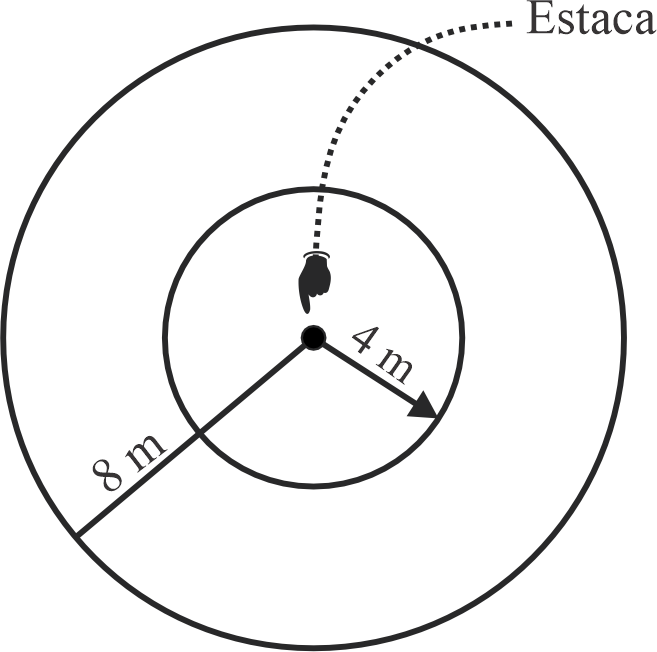
\includegraphics[width=3.5cm]{imagenes/general2024-I/etapa1/ing/RM3g24-I.png}
	\end{minipage}
\end{center}








\item Si $ABCD$ es un cuadrado de lado $4$ m, calcule el perímetro de la región sombreada.

\begin{center}
	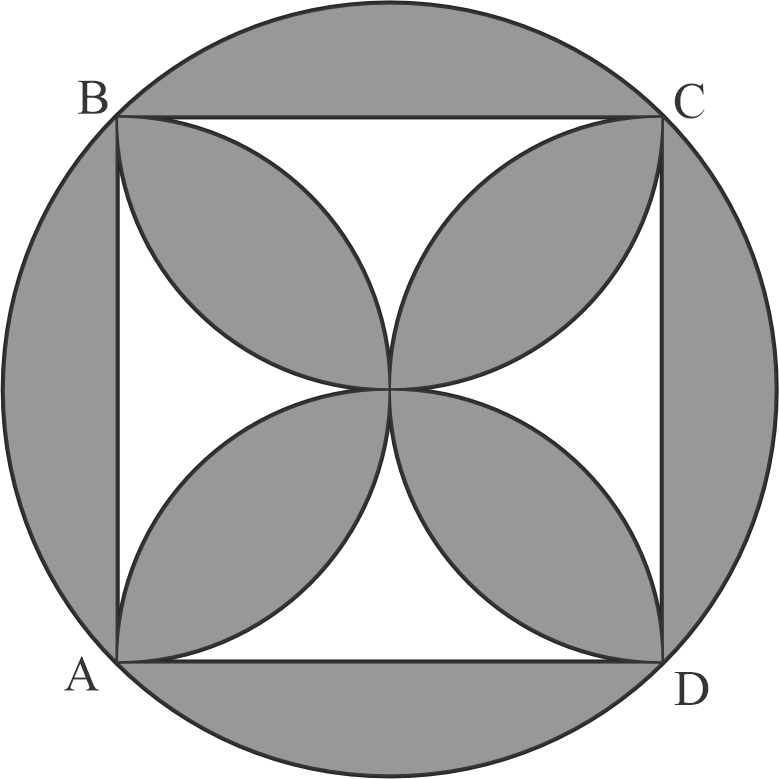
\includegraphics[width=3.5cm]{imagenes/general2024-I/etapa1/ing/RM4g24-I.png} % Ajusta el nombre según tu archivo
\end{center}

\begin{enumerate}[label=\alph*)]
	\item $4(\pi + 2\pi + 4)$ m
	\item $4(\sqrt{2}\pi + 2\pi + 4)$ m
	\item $4(2\sqrt{2}\pi + \pi + 4)$ m
	\item $8(2\sqrt{2}\pi + 2\pi + 2)$ m
	\item $8(4\sqrt{2}\pi + \pi + 2)$ m
\end{enumerate}

\textbf{Respuesta correcta:} b)

\vspace{4mm}
\textbf{Solucionario:}\\[1mm]


\begin{center}
	\begin{minipage}{0.45\textwidth}
		\item[i)] \textbf{Del Grafico}\\
		\item[ii)] \textbf{Perimetro cuadrado}\\
		$= 16 \text{ m}$\\
		\item[iii)] \textbf{Circunferencia}\\
		$P = 2\pi r = 2\pi (2\sqrt{2}) = 4\sqrt{2}\pi$\\
		$\text{perimetro arcos} \left( \begin{array}{l} 
			\stackrel{\frown}{AB} = 2\pi \\
			\stackrel{\frown}{CD} = 2\pi \\
			\stackrel{\frown}{BC} = 2\pi \\
			\stackrel{\frown}{AD} = 2\pi 
		\end{array} \right. = 8\pi$
		
		\vspace{4mm}
		$\therefore \textbf{perímetro} = (4\sqrt{2}\pi + 8\pi + 16)m$ \\
		\hspace{20mm} $= 4(\sqrt{2}\pi + 2\pi + 4)m$
		
	\end{minipage}
	\hfill
	\begin{minipage}{0.45\textwidth}
		\centering
		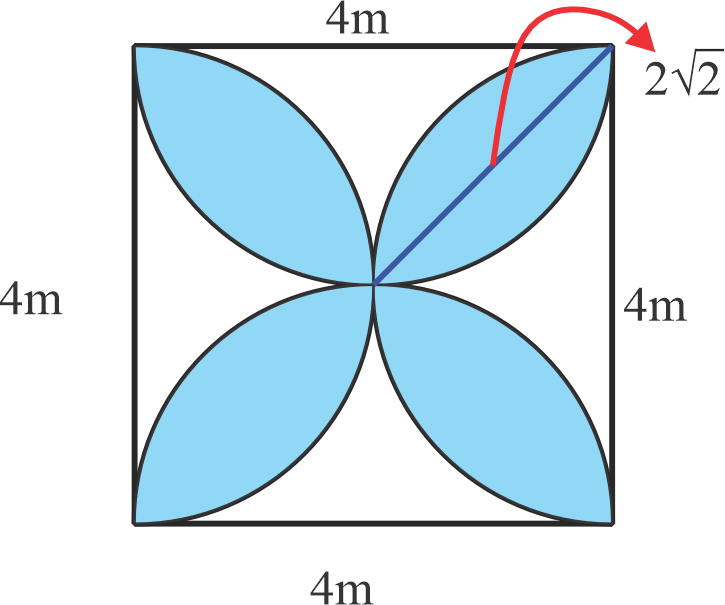
\includegraphics[width=4cm]{imagenes/general2024-I/etapa1/ing/RM4g24r-I.png} 
	\end{minipage}
\end{center}

	\item Se define el operador:
	$$2a^b \circledast 3b^a = \sqrt{a^2 + b^2}$$
	Halle: $128 \circledast 243$
	
	\begin{enumerate}[label=\alph*)]
		\item 5
		\item 3
		\item 4
		\item 7
		\item 6
	\end{enumerate}
	
	\textbf{Respuesta correcta:} a)
	
	\vspace{2mm}
	\textbf{Solucionario:}\\[1mm]
	Dando la forma de la definición:\\
	$$128 \circledast 243 = 2 \cdot 4^3 \circledast 3 \cdot 3^4$$\\
	De donde se obtiene que:\\
	$a = 4$ y $b = 3$\\
	
	Remplazando:\\
	$\Rightarrow \sqrt{4^2 + 3^2}$\\
	$= \sqrt{16 + 9} = \sqrt{25} = 5$\\
	
	\vspace{6mm}


	\item Calcule la suma:
	$$S = 25 + 36 + 49 + \dots + 400$$
	
	\begin{enumerate}[label=\alph*)]
		\item 2810
		\item 2820
		\item 2830
		\item 2840
		\item 2850
	\end{enumerate}
	
	\textbf{Respuesta correcta:} d)
	
	\vspace{2mm}
	\textbf{Solucionario:}\\[1mm]
	\underline{(Fórmula)}
	$$\sum_{i=1}^{n} i^2 = \dfrac{n(n+1)(2n+1)}{6}$$
	
	Identificando los términos de la serie:
	$$S = \sum_{i=1}^{20} i^2 - \sum_{i=1}^{4} i^2 = (1^2 + 2^2 + 3^2 + \dots + 20^2) - (1^2 + 2^2 + 3^2 + 4^2)$$
	
	Aplicando la fórmula para $n=20$ y $n=4$:
	$$= \dfrac{20(20+1)(2(20)+1)}{6} - \dfrac{4(4+1)(2(4)+1)}{6}$$
	$$= 2870 - 30$$
	$$= 2840$$
	
	\vspace{6mm}
	
	
\end{enumerate}





\subsection*{Razonamiento Verbal}

\begin{enumerate}[resume]
	
	\item La palabra ingeniero proviene del latín \textit{ingenium} que significa:
	
	\begin{enumerate}[label=\alph*)]
		\item Poseer o estimular la capacidad de creación, invención, etc.
		\item Adaptarse frente a un agente perturbador, estado o situación adverso.
		\item Discurrir o inventar con prontitud y facilidad.
		\item Emprender con resolución, acciones o empresas innovadoras.
		\item Poseer los conocimientos especiales de una ciencia o arte.
	\end{enumerate}
	
	\textbf{Respuesta correcta:} c)
	
	\vspace{2mm}
	\textbf{Solucionario:}\\[1mm]
	Etimológicamente, \textit{ingenium} se refiere a la cualidad natural de una persona para crear o dar soluciones ingeniosas. La definición que mejor se ajusta a esta raíz es la capacidad de discurrir o inventar de manera rápida y eficaz ante un desafío.
	
	\vspace{6mm}
	
	\item Complete la oración:
	
	No logró ingresar a la universidad \_\_\_\_\_\_\_ de haberse preparado adecuadamente, \_\_\_\_\_\_\_, su perseverancia será recompensada en algún momento.
	
	\begin{enumerate}[label=\alph*)]
		\item no obstante \textemdash por lo tanto
		\item a pesar \textemdash sin embargo
		\item luego \textemdash por lo que
		\item después \textemdash entonces
		\item empero \textemdash pero
	\end{enumerate}
	
	\textbf{Respuesta correcta:} b)
	
	\vspace{2mm}
	\textbf{Solucionario:}\\[1mm]
	El primer espacio requiere un conector concesivo ("a pesar") que indique que el resultado fue adverso pese a la preparación. El segundo espacio requiere un conector adversativo ("sin embargo") para introducir la idea de esperanza en la perseverancia futura.
	
	\vspace{6mm}
	
	\item Encuentre la oración a eliminar:
	
	I. La situación económica del Perú es el resultado de borrones y cuentas nuevas en la política peruana. \\
	II. Cada nueva administración gubernamental trata de desaparecer los vestigios de la anterior. \\
	III. De lo que se trata es concertar un proyecto de desarrollo que todos los partidos respeten. \\
	IV. De este modo se podrá planificar para el futuro programas de mediano y largo plazo. \\
	V. La concentración es básicamente un nivel de acuerdo.
	
	\begin{enumerate}[label=\alph*)]
		\item IV
		\item II
		\item V
		\item I
		\item III
	\end{enumerate}
	
	\textbf{Respuesta correcta:} c)
	
	\vspace{2mm}
	\textbf{Solucionario:}\\[1mm]
	El texto trata sobre la falta de continuidad política y la necesidad de proyectos de desarrollo a largo plazo. La oración V se elimina por impertinencia, ya que define "concentración" de forma aislada, alejándose del eje temático sobre administración pública y planificación.
	
	\vspace{6mm}
	
	\item Identifica el par analógico.
	
	SEDIMENTACIÓN : ESTRATO ::
	
	\begin{enumerate}[label=\alph*)]
		\item erosión : desgaste.
		\item ciencia : estudio.
		\item ficción : realidad.
		\item nobleza : verdad.
		\item base : capa.
	\end{enumerate}
	
	\textbf{Respuesta correcta:} e)
	
	\vspace{2mm}
	\textbf{Solucionario:}\\[1mm]
	La relación es de proceso a producto: la sedimentación genera el estrato (una capa de sedimentos). De manera análoga, una base constituye el fundamento o soporte de una capa en diversas estructuras o formaciones.
	
	\vspace{6mm}
	
	\item PLAN DE REDACCIÓN \\
	\textbf{Galileo Galilei}
	
	I. Realizó experiencias sobre la caída de los cuerpos e inventó el termómetro. \\
	II. Fue matemático, físico y astrónomo y el verdadero fundador de la Física y la Mecánica. \\
	III. A los 19 años, observó en la Catedral de Pisa, una lámpara que se balanceaba colgada de la cúpula y se le ocurrió aplicar el péndulo a la medida del tiempo. \\
	IV. Partidario del sistema de Copérnico, abjuró de sus convicciones sobre el movimiento de la tierra obligado por la inquisición. \\
	V. Por ello, Galileo es considerado como el prototipo de mártir a causa de la ciencia.
	
	\begin{enumerate}[label=\alph*)]
		\item II - I - III - IV - V
		\item II - III - IV - I - V
		\item III - II - I - IV - V
		\item III - II - I - V - IV
		\item IV - V - I - II - III
	\end{enumerate}
	
	\textbf{Respuesta correcta:} d)
	
	\vspace{2mm}
	\textbf{Solucionario:}\\[1mm]
	El orden lógico sigue un criterio cronológico y de relevancia: se inicia con su juventud (III), se define su importancia general (II), se mencionan sus inventos y experimentos (I), se concluye con el impacto de su juicio (V) y su conflicto final con la inquisición (IV).
	
	\vspace{6mm}
	
	\item Los ríos se caracterizan por su baja productividad primaria y baja concentración de oxígeno disuelto. Sin embargo, en ellos vive un gran número de poblaciones de animales debido a que la corriente del río carga materiales orgánicos de otros sistemas y ventila los organismos sosteniéndolos a pesar de las condiciones antes referidas. Aplicando el modelo producción  respiración, el río es un sistema heterotrófico, donde la respiración es mayor que la producción. La productividad primaria del río radica principalmente en la superficie de las rocas o en los lentos remansos, donde la poca velocidad de las aguas permite el crecimiento de algas o de plantas acuáticas vasculares desde el punto de vista regional los ríos transportan con rapidez materiales y energía entre un sistema y otro.
	
	Pese a sus deficientes condiciones, los ríos pueden sostener vida gracias a que:
	
	\begin{enumerate}[label=\alph*)]
		\item Son subsidiados por lagos.
		\item La agitación mecánica arrastra e incorpora al río lo necesario.
		\item El río tiene zonas tranquilas, los remansos favorables a la vida.
		\item La respiración es mayor que la producción.
		\item Los organismos se han adaptado a esas duras condiciones.
	\end{enumerate}
	
	\textbf{Respuesta correcta:} b)
	
	\vspace{2mm}
	\textbf{Solucionario:}\\[1mm]
	Según el texto, la corriente del río carga materiales orgánicos y ventila los organismos. Esta "agitación mecánica" permite la incorporación de nutrientes y oxígeno de otros sistemas, compensando la baja productividad primaria propia del río.
	
	\vspace{6mm}
	
\end{enumerate}


\subsection*{Inglés}

\begin{enumerate}[resume]

	\item Answer the question about the underline word.
	"The mothers day is \underline{in} May on the second Sunday"
	What is underline word?
	
	\begin{enumerate}[label=\alph*)]
		\item Preposition
		\item Verb
		\item Gerund
		\item Noun
		\item Simple
	\end{enumerate}
	
	\textbf{Respuesta correcta:} a)
	
	\vspace{2mm}
	\textbf{Solucionario:}\\[1mm]
	En la gramática inglesa, "in" es una preposición de tiempo que se utiliza antes de meses, años, siglos y períodos largos. En la oración proporcionada, establece la relación temporal entre el Día de la Madre y el mes de mayo.
	
	\vspace{6mm}
	
	\item Select the option with the irregular verb in the simple past tense.
	
	\begin{enumerate}[label=\alph*)]
		\item I lived to dance
		\item We live in Puno
		\item We meet en the afternoon
		\item I enjoyed singing with him
		\item I had two sisters
	\end{enumerate}
	
	\textbf{Respuesta correcta:} e)
	
	\vspace{2mm}
	\textbf{Solucionario:}\\[1mm]
	Los verbos irregulares son aquellos que no siguen la regla estándar de añadir "-ed" para formar el tiempo pasado. El verbo "had" es el pasado del verbo irregular "have". Las otras opciones utilizan verbos regulares en pasado ("lived", "enjoyed") o están en tiempo presente ("live", "meet").
	
	\vspace{6mm}
	
\end{enumerate}





\subsection*{Quechua y Aimara}

\begin{enumerate}[resume]
	
	\item Ñuqaq kimsa chunka uwihaykuna karqan, kimsata atuq mikhurqapusqa, ¿Hayk'a uwihakunataq qhipawan?/Nayaxa kimsatunka uwijaniyatwa. Kimsaru qamaqi manq'antawayi. ¿Qawqhasa jichaxa utjaski?
	
	\begin{enumerate}[label=\alph*)]
		\item Iskay chunka pichqayuq/Pä tunka phisqani.
		\item Iskay chunka suqtayuq/Pä tunka suxtani.
		\item Iskay chunka qanchisniyuq/Pä tunka paqallquni.
		\item Iskay chunka pusaqniyuq/Pä tunka kimsaqallquni.
		\item Iskay chunka isqunniyuq/Pä tunka llatunkani.
	\end{enumerate}
	
	\textbf{Respuesta correcta:} c)
	
	\vspace{2mm}
	\textbf{Solucionario:}\\[1mm]
	El problema plantea una resta básica en Quechua y Aimara: "Tenía 30 ovejas (\textit{kimsa chunka} / \textit{kimsatunka}) y el zorro se comió 3 (\textit{kimsa} / \textit{kimsa})". 
	Operación: $30 - 3 = 27$.
	En Quechua, 27 es \textit{Iskay chunka qanchisniyuq} y en Aimara es \textit{Pä tunka paqallquni}.
	
	\vspace{6mm}
	
	\item Chunkaman tawata yapaykuptiyri, ¿Hayk'ataq kanman?/Tunkaru pusimpi apxatirista, ¿Ukaxa qawqhaspasa?
	
	\begin{enumerate}[label=\alph*)]
		\item Chunka hukniyuq/Tunka mayani.
		\item Chunka iskayniyuq/Tunka payani.
		\item Chunka kimsayuq/Tunka kimsani.
		\item Chunka tawayuq/Tunka pusini.
		\item Chunka pichqayuq/Tunka phisqani.
	\end{enumerate}
	
	\textbf{Respuesta correcta:} d)
	
	\vspace{2mm}
	\textbf{Solucionario:}\\[1mm]
	La pregunta solicita realizar una suma: "A diez (\textit{chunka} / \textit{tunka}) le agrego cuatro (\textit{tawa} / \textit{pusi}), ¿cuánto sería?".
	Operación: $10 + 4 = 14$.
	En Quechua, 14 se dice \textit{Chunka tawayuq} y en Aimara se dice \textit{Tunka pusini}.
	
	\vspace{6mm}
	
\end{enumerate}

\section*{Área: Biomédicas}


\subsection*{Aritmética}

\begin{enumerate}
	
	\item Determine el esquema mólecular simplificado del siguiente circuito:
	
	
	\begin{figure}[h]
		\centering
		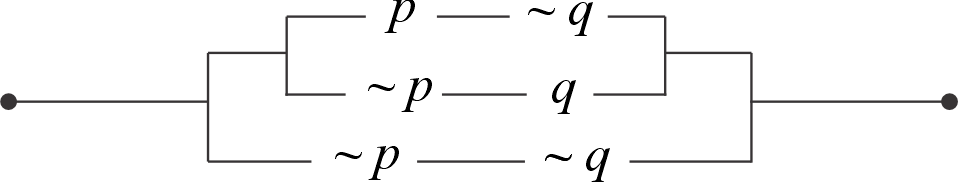
\includegraphics[width=0.6\textwidth]{imagenes/general2024-I/etapa1/bio/aritmetica1g24-I}
		%\caption{Descripción de la imagen}
		%\label{fig:ejemplo}
	\end{figure}
	
	
	
	
	\begin{enumerate}[label=\alph*)]
		\item $p \land q$
		\item $p \lor q$
		\item $\sim p\,\,\land \sim q$
		\item $\sim p\,\,\lor \sim q$
		\item $\sim p\,\land q$
	\end{enumerate}
	
	\textbf{Respuesta correcta:} d)
	
	\vspace{2mm}
	\textbf{Solucionario:}\\[1mm]
	Del circuito inicial podemos formar lo siguiente, reduciendo:
	
	\begin{figure}[h]
		\centering
		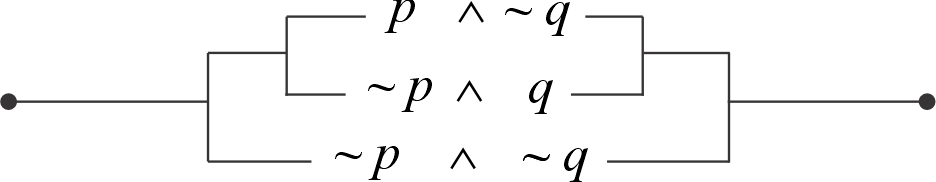
\includegraphics[width=0.6\textwidth]{imagenes/general2024-I/etapa1/bio/aritmetica1soluciong24-I}
		%\caption{Descripción de la imagen}
		%\label{fig:ejemplo}
	\end{figure}
	
	
	De ahí tendremos la siguiente expresión lógica:
	
	\[\begin{array}{l}
		\equiv [(p \,\wedge  \sim q) \vee ( \sim p \wedge q)] \vee ( \sim p \wedge  \sim q)\\
		\equiv [(p \vee ( \sim p \wedge q)) \wedge ( \sim q \vee ( \sim p \wedge q))] \vee  \sim (p \wedge q)\\
		\equiv [(p \vee q) \wedge ( \sim q\, \vee  \sim p)] \vee  \sim (p \wedge q)\\
		\equiv ( \sim q\, \vee  \sim p) \vee ( \sim p\, \wedge  \sim q)\\
		\equiv  \sim q \vee [ \sim p \vee ( \sim p \,\wedge  \sim q)] \\ \equiv  \sim q\, \vee  \sim p\, \\ \equiv  \sim p\, \vee  \sim q
	\end{array}\]
	
	
	\vspace{6mm}
	
	\item Un cilindro de 60L de capacidad, fue llenado completamente por 4 recipientes donde el volumen del primero es al segundo como el del tercero es al cuarto como 2 es a 1. Halle la suma de los volúmenes del segundo y cuarto recipiente.
	\begin{enumerate}[label=\alph*)]
		\item 20L
		\item 30L
		\item 40L
		\item 15L
		\item 25L
	\end{enumerate}
	
	\textbf{Respuesta correcta:} a)
	
	\vspace{2mm}
	\textbf{Solucionario:}\\[1mm]
	$V_1$ + $V_2$ + $V_3$ + $V_4$ = 60\\
	
	$\displaystyle\dfrac{V_1}{V_2} = \dfrac{V_3}{V_4} = \dfrac{2}{1}$\\
	
	$\displaystyle\dfrac{V_1+V_3}{V_2+V_4} = \dfrac{2}{1}$\\
	
	Propiedad   $\displaystyle\dfrac{V_1+V_2+V_3+V_4}{V_2+V_4} = \dfrac{2+1}{1}$\\
	
	Reemplazando   $\displaystyle\dfrac{60}{V_2+V_4} = \dfrac{3}{1}$\\
	
	Donde $V_2$ + $V_4$ = 20L
	
	\vspace{6mm}
	
	\item El dinero de A excede al de B en 20\% del dinero de C y el exceso de B a C equivaleal 10\% del dinero de A. Si A tiene S/.200 ¿Cuantos tiene C y B juntos? 
	
	
	
	
	\begin{enumerate}[label=\alph*)]
		\item 280
		\item 300
		\item 420
		\item 360
		\item 320
	\end{enumerate}
	
	\textbf{Respuesta correcta:} e)
	
	\vspace{2mm}
	\textbf{Solucionario:}\\[1mm]
	
	A = S/.200 B=3 C=?\\
	
	A - B = 20\%C ...... (1)\\
	B - C = 10\%A ...... (2)\\
	A - C = 20\%C + 10\%A
	
	100\%A - 100\%C = 20\%C + 10\%A\\
	90\%A = 120\%C\\
	90\%A = 120\%C
	
	90(200) = 120C => C = S/.150
	
	En(1) 200 - B =  $\displaystyle\dfrac{20}{100}$(150) = S/.170 = B
	
	A + B = 150 + 170 = 320
	
	
	
	\vspace{6mm}
	
\end{enumerate}



\subsection*{Álgebra}

\begin{enumerate}[resume]
	
	\item En el polinomio P(x)=$(1+2x)^n$+$(1+3x)^n$, la suma de coeficientes excede en 23 al término independiente. Según ello, establezca el valor de verdad de las siguientes proposiciones:
	\begin{enumerate}[label=\Roman*.]
		\item El polinomio es de grado 2
		\item La suma de sus coeficientes es 25
		\item El término cuadrático es $12x^2$
	\end{enumerate}
	
	
	\begin{enumerate}[label=\alph*)]
		\item VVV
		\item VFV
		\item VVF
		\item FVV
		\item FFV
	\end{enumerate}
	
	\textbf{Respuesta correcta:} c)
	
	\vspace{2mm}
	\textbf{Solucionario:}\\[1mm]
	
	$P(1)=3^n+4^n$ ; $P(0)=1+1=2$\\
	$P(1)=P(0)+23$\\
	$3^n+4^n=2+23=25$\\    
	$\therefore n = 2$\\
	$P(x)=1+4x+4x^2+1+6x+9x^2$\\
	$P(x)=13x^2+10x+2; P(1)=25$\\
	
	\begin{itemize}[label=*]
		\item El polinomio $P(x)$ es de grado 2.(V)
		\item La suma de sus coeficientes es 25 (V)
		\item El término cuadrático de $P(x)$ es $12x^2$. (F)
	\end{itemize}
	
	
	
	
\end{enumerate}

\begin{enumerate}[resume]
	
	\item Sabiendo que:
	${x^3} + \dfrac{1}{{{y^3}}} = {y^3} + \dfrac{1}{{{z^3}}} = 1$\\
	Calcule $(xyz)^{102}-1$
	
	
	\begin{enumerate}[label=\alph*)]
		\item $\,\,\,\,2$
		\item $-1$
		\item $\,\,\,\,0$
		\item $\,\,\,\,1$
		\item $-2$
	\end{enumerate}
	
	\textbf{Respuesta correcta:} c)
	
	\vspace{2mm}
	\textbf{Solucionario:}\\[1mm]
	
	${x^3} + \dfrac{1}{{{y^3}}} = 1 \Rightarrow {x^3}{y^3} + 1 = {y^3}$\\
	${y^3} = 1 - \dfrac{1}{{{z^3}}}\,\,\,luego\,\,{x^3}{y^3} + 1 = 1 - \dfrac{1}{{{z^3}}}$\\
	${x^3}{y^3} =  - \dfrac{1}{{{z^3}}}\,\, \Rightarrow \,\,\,{x^3}{y^3}{z^3} =  - 1$\	de donde ${\left( {{x^3}{y^3}{z^3}} \right)^{34}} = {\left( { - 1} \right)^{34}} = 1$\\\\
	$\therefore {(xyz)^{102}} - 1 = 1 - 1 = 0$
	
	
\end{enumerate}


\begin{enumerate}[resume]
	
	\item Sea la función $f = [5,b] \to [a,5]$, cuya regla de correspondencia es $f(x)=x^2-6x+1$. Calcule el valor de $a+b$ siendo $f$ biyectiva. 
	\begin{enumerate}[label=\alph*)]
		\item $\sqrt{13}-1$
		\item $\sqrt{13}-2$
		\item $\sqrt{13}+2$
		\item $\sqrt{13}+1$
		\item $\sqrt{13}+3$
	\end{enumerate}
	
	\textbf{Respuesta correcta:} a)
	
	\vspace{2mm}
	\textbf{Solucionario:}\\[1mm]
	
	$f(x)=x^2-6x+1=(x-3)^2-8$\\
	$f$ es creciente $f(5)=a$ y $f(b)=5$
	
	\begin{itemize}[label=.]
		\item $25 - 30 + 1 = a\Rightarrow a =  - 4$
		\item $(b + 3)^2 - 8 = 5 \Rightarrow {(b + 3)^2} = 13 \Rightarrow b = 3 + \sqrt {13}$
		
	\end{itemize}
	
	luego $a+b=\sqrt{13}-1$
	
\end{enumerate}



\subsection*{Geometría}

\begin{enumerate}[resume]
	
	\item En la figura, calcule la	$m \overset{\frown}{EF}$
	
	
	\begin{figure}[h]
		\centering
		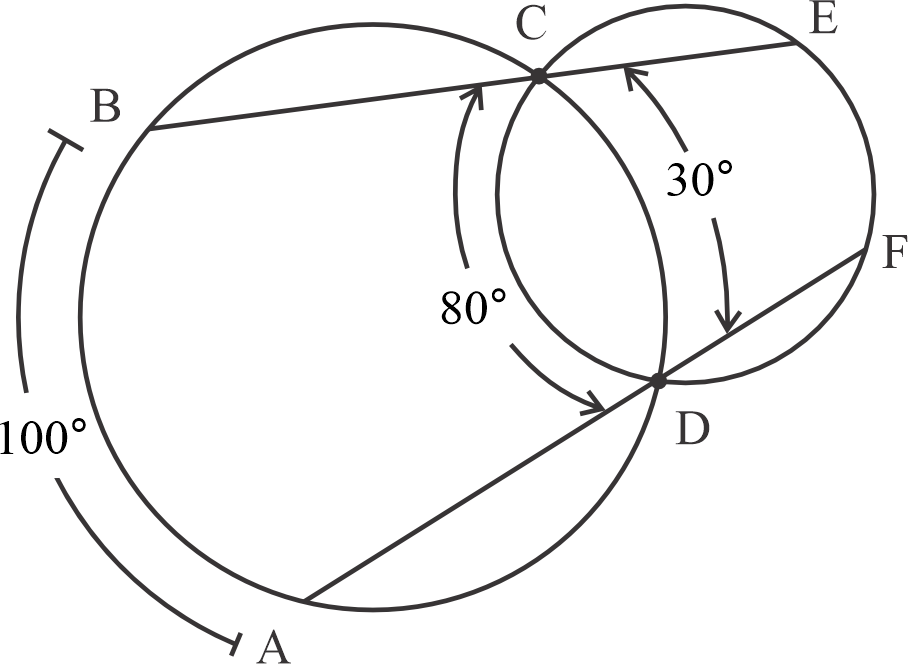
\includegraphics[width=0.3\textwidth]{imagenes/general2024-I/etapa1/bio/geometria1g24-I}
		%\caption{Descripción de la imagen}
		%\label{fig:ejemplo}
	\end{figure}
	
	\begin{enumerate}[label=\alph*)]
		\item $10^\circ$
		\item $20^\circ$
		\item $35^\circ$
		\item $45^\circ$
		\item $50^\circ$
	\end{enumerate}
	
	\textbf{Respuesta correcta:} a)
	
	\vspace{2mm}
	
	\noindent
	\begin{minipage}[t]{0.3\textwidth}
		\vspace{1pt}
		\textbf{Solucionario:}\\[1mm]
		
		De la figura:\\
		
		$\alpha=\dfrac{{100 - 30}}{2} = 35^\circ$\\
		$\alpha  = \dfrac{{80 - x}}{2}$\\
		
		$\to x = 80 - 2\alpha$\\
		$x=80 - 2(35)$\\
		$x = 10^\circ$	
		
	\end{minipage}
	\hfill
	\begin{minipage}[t]{0.7\textwidth}
		\vspace{0pt}
		\centering
		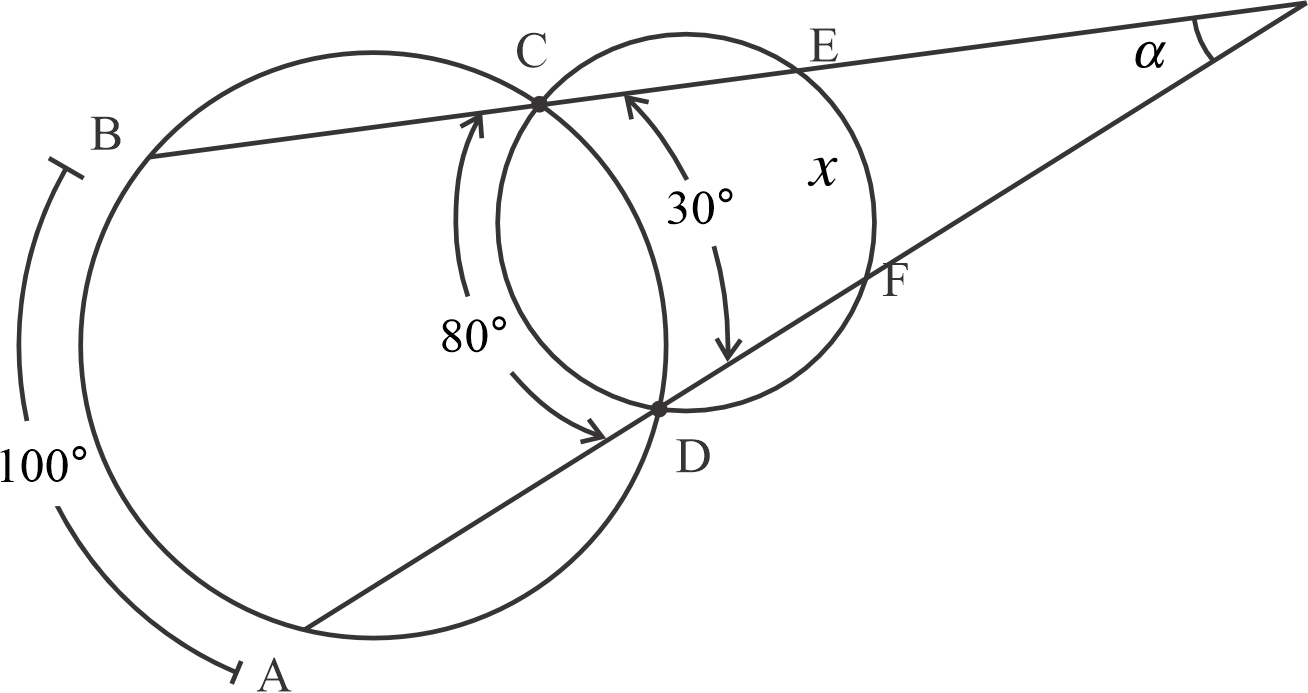
\includegraphics[width=0.7\textwidth]{imagenes/general2024-I/etapa1/bio/geometria1soluciong24-I}
	\end{minipage}
	
	
	
	
	
	
\end{enumerate}



\begin{enumerate}[resume]
	
	\item En la figura	PUNO y UNAP son cuadrados. Si $\alpha=16^\circ$, calcule $x$.
	
	
	\begin{figure}[h]
		\centering
		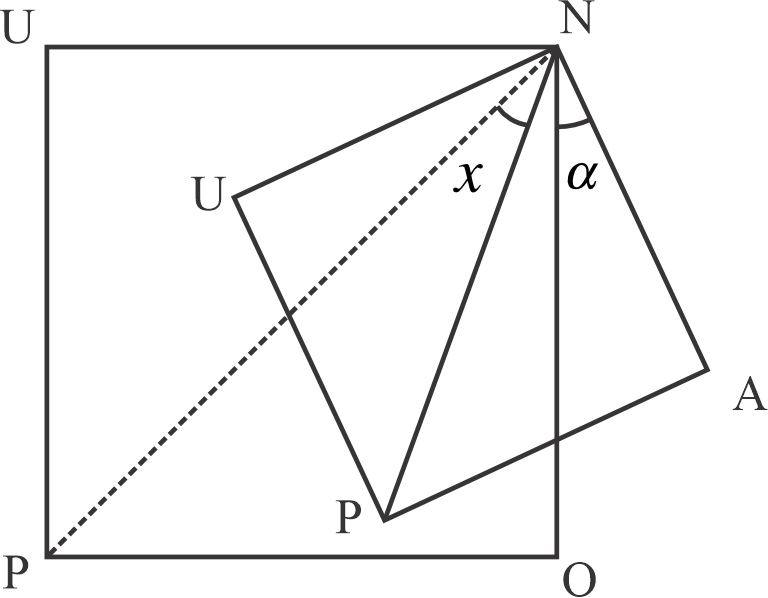
\includegraphics[width=0.37\textwidth]{imagenes/general2024-I/etapa1/bio/geometria2g24-I}
		%\caption{Descripción de la imagen}
		%\label{fig:ejemplo}
	\end{figure}
	
	
	\begin{enumerate}[label=\alph*)]
		\item $15^\circ$
		\item $16^\circ$
		\item $22^\circ$
		\item $31^\circ$
		\item $35^\circ$
	\end{enumerate}
	
	
	\vspace{2mm}
	\textbf{Respuesta correcta:} b)
	
	\vspace{2mm}
	
	
	
	\noindent
	\begin{minipage}[t]{0.3\textwidth}
		\vspace{2pt}
		\textbf{Solucionario:}\\[1mm]
		
		De la figura:\\\\
		${45^\circ } - x + \alpha  = {45^\circ }\\
		x = \alpha \\
		x = 16^\circ$	
		
	\end{minipage}
	\hfill
	\begin{minipage}[t]{0.7\textwidth}
		\vspace{0pt}
		\centering
		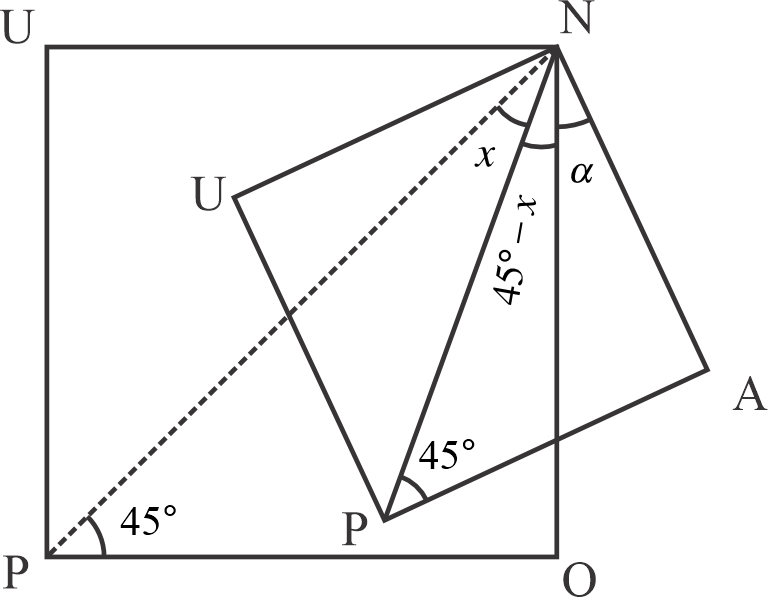
\includegraphics[width=0.55\textwidth]{imagenes/general2024-I/etapa1/bio/geometria2soluciong24-I}
	\end{minipage}
	
	
\end{enumerate}


\begin{enumerate}[resume]
	
	\item Determine la ecuación de la recta que contiene al diamétro de la circunferencia $x^2+y^2-4x-6y=17$ que es perpendicular a la recta $L:5x-2y=13$.
	\begin{enumerate}[label=\alph*)]
		\item $2x+5y-19=0$
		\item $5x+2y-19=0$
		\item $2x-5y-19=0$
		\item $2x+5y+11=0$
		\item $5x+2y+11=0$
	\end{enumerate}
	
	\textbf{Respuesta correcta:} a)
	
	\vspace{2mm}
	\textbf{Solucionario:}\\[1mm]
	
	$x^2+y^2-4x-6y=17\\
	{x-2}^2+{y-3}^2=17+4+9\\
	{x-2}^2+{y-3}^2=30\\
	c=(2,3)\\$
	
	$L:2y =  - 13 + 5x$
	
	$\,\,\,\,\,\,\,\,\,y =  + \dfrac{5}{2}x - \dfrac{{13}}{2} \to {m_1} =  + \dfrac{5}{2}\\$
	
	
	${L_p}:y - {y_0} =  - \dfrac{2}{5}(x - {x_0})$
	
	$\,\,\,\,\,\,\,\,\,5y + 2x + b = 0$
	
	$\,\,\,\,\,\,\,\,5(3) + 2(2) + b = 0$
	
	$\,\,\,\,\,\,\,\,b =  - 19\\$
	
	$\therefore {L_{perpendicular}} : 2x + 5y - 19 = 0$
	
	
	
	
\end{enumerate}


\subsection*{Trigonometría}

\begin{enumerate}[resume]
	
	\item En el gráfico, calcule el área de la región sombreada. 
	
	\begin{figure}[h]
		\centering
		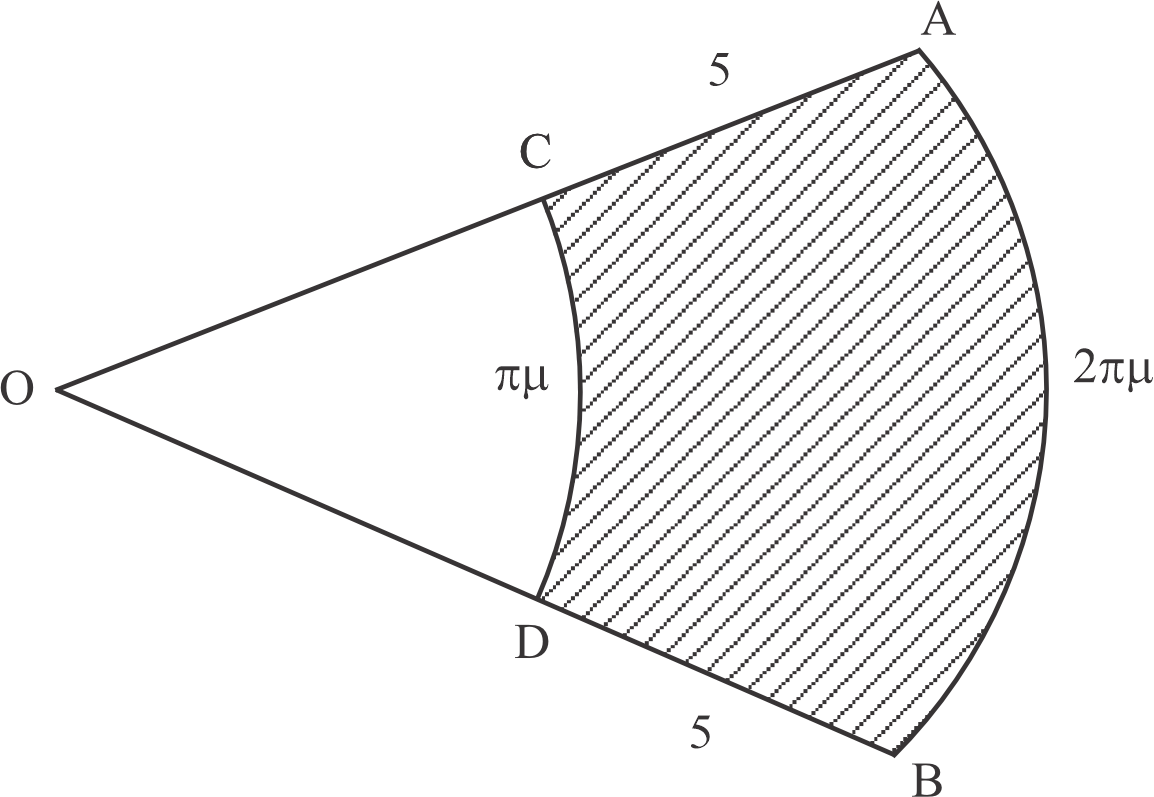
\includegraphics[width=0.48\textwidth]{imagenes/general2024-I/etapa1/bio/trigonometria1g24-I}
		%\caption{Descripción de la imagen}
		%\label{fig:ejemplo}
	\end{figure}
	
	\begin{enumerate}[label=\alph*)]
		\item $\dfrac{{5\pi }}{2}{\mu ^2}$
		\item $\dfrac{{13\pi }}{2}{\mu ^2}$
		\item $\dfrac{{9\pi }}{2}{\mu ^2}$
		\item $\dfrac{{15\pi }}{2}{\mu ^2}$
		\item $\dfrac{{11\pi }}{2}{\mu ^2}$
	\end{enumerate}
	
	\textbf{Respuesta correcta:} d)
	
	\vspace{2mm}
	\textbf{Solucionario:}
	
	\noindent
	\begin{minipage}[t]{0.3\textwidth}
		\vspace{2pt}
		De la figura:\\\\
		${A_S} = \left( {\dfrac{{2\pi  + \pi }}{2}} \right)(5)\\\\
		{A_S} = \left( {\dfrac{{3\pi}}{2}} \right)(5)\\\\
		{A_S} = \dfrac{{15\pi }}{2}{\mu ^2}$	
		
	\end{minipage}
	\hfill
	\begin{minipage}[t]{0.7\textwidth}
		\vspace{0pt}
		\centering
		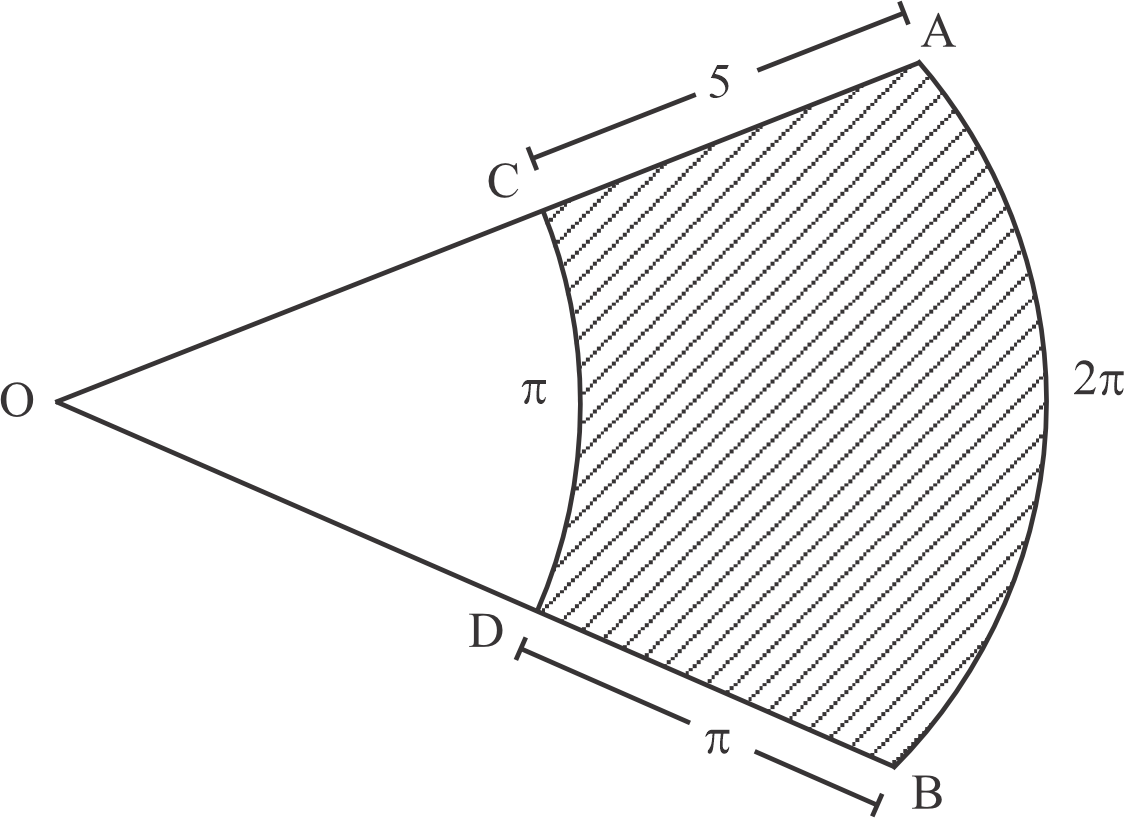
\includegraphics[width=0.65\textwidth]{imagenes/general2024-I/etapa1/bio/trigonometria1soluciong24-I}
	\end{minipage}
	
	
	
\end{enumerate}



\begin{enumerate}[resume]
	
	\item Si A y B son ángulos suplementarios, calcule:
	\[M=cos^2A+sen^2B\]
	\begin{enumerate}[label=\alph*)]
		\item $\,\,\,\,0$
		\item $\,\,\,\,\dfrac{1}{2}$
		\item $\,\,\,\,1$
		\item $-1$
		\item $-\dfrac{1}{2}$
	\end{enumerate}
	
	\textbf{Respuesta correcta:} c)
	
	\vspace{2mm}
	\textbf{Solucionario:}
	
	$A+B=180^\circ\\
	B=180^\circ-A$
	
	$M=cos^2A+sen^2B\\
	M=cos^2A+sen^2(180^\circ-A)\\
	M=cos^2A+(-senA)^2\\
	M=cos^2A+sen^2A\\
	M=1$
	
\end{enumerate}




\begin{enumerate}[resume]
	
	\item En el gráfico, AB$=6$; BC$=5$ y AC$=4$
	
	
	\begin{figure}[h]
		\centering
		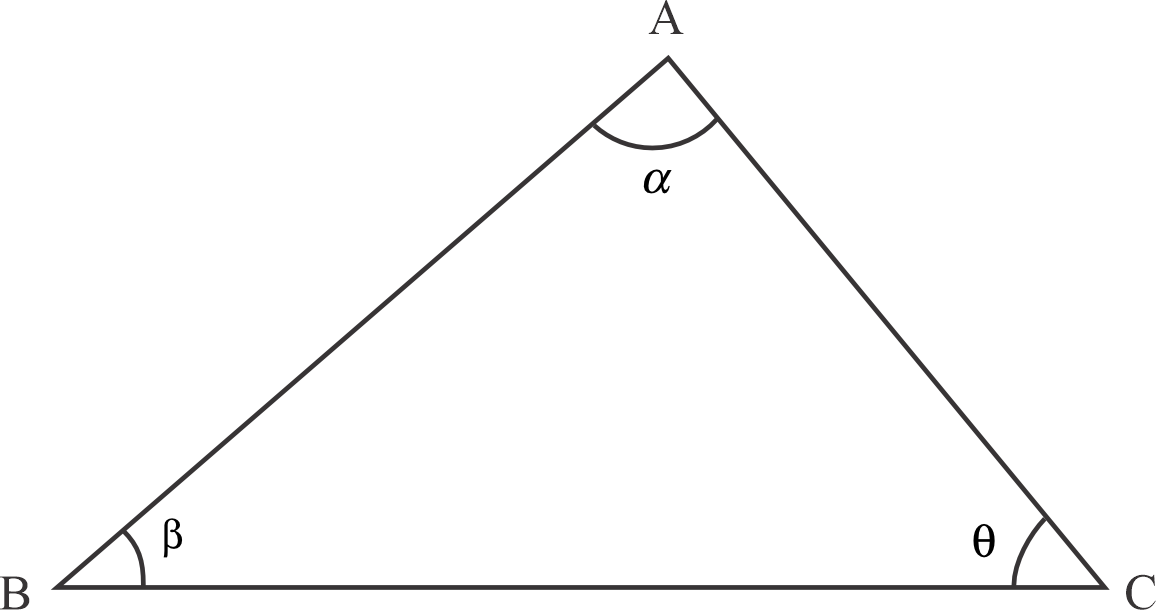
\includegraphics[width=0.5\textwidth]{imagenes/general2024-I/etapa1/bio/trigonometria3g24-I}
		%\caption{Descripción de la imagen}
		%\label{fig:ejemplo}
	\end{figure}
	
	
	Calcule:
	\[M = \dfrac{{sen\alpha  + sen\beta }}{{sen\theta }}\]
	
	\begin{enumerate}[label=\alph*)]
		\item $\dfrac{4}{3}$
		\item $\dfrac{3}{2}$
		\item $\dfrac{3}{4}$
		\item $\dfrac{2}{3}$
		\item $\dfrac{2}{5}$
	\end{enumerate}
	
	\textbf{Respuesta correcta:} b)
	
	\vspace{2mm}
	\textbf{Solucionario:}\\[1mm]
	
	\noindent
	\begin{minipage}[t]{0.35\textwidth}
		\vspace{2pt}
		Ley de senos:\\
		
		$M = \dfrac{{4}}{{sen\beta }}+\dfrac{{5}}{{sen\alpha }}+\dfrac{{6}}{{sen\theta }}=2R\\\\
		M=\dfrac{{sen\beta}}{{4}}+\dfrac{{sen\alpha}}{{5}}+\dfrac{{sen\theta}}{{6}}=\dfrac{{1}}{{2R}}$
		
		$ \left\{ {\begin{array}{*{20}{c}}
				sen\beta=\dfrac{{4}}{{2R}}\\\\
				sen\alpha=\dfrac{{5}}{{2R}}\\\\
				sen\theta=\dfrac{{6}}{{2R}}
		\end{array}} \right.$
		
		$M = \dfrac{{\dfrac{5}{{2R}} + \dfrac{4}{{2R}}}}{{\dfrac{6}{{2R}}}} = \dfrac{{\dfrac{9}{{2R}}}}{{\dfrac{6}{{2R}}}} = \dfrac{9}{6} = \dfrac{3}{2}$	
		
	\end{minipage}
	\hfill
	\begin{minipage}[t]{0.65\textwidth}
		\vspace{0pt}
		\centering
		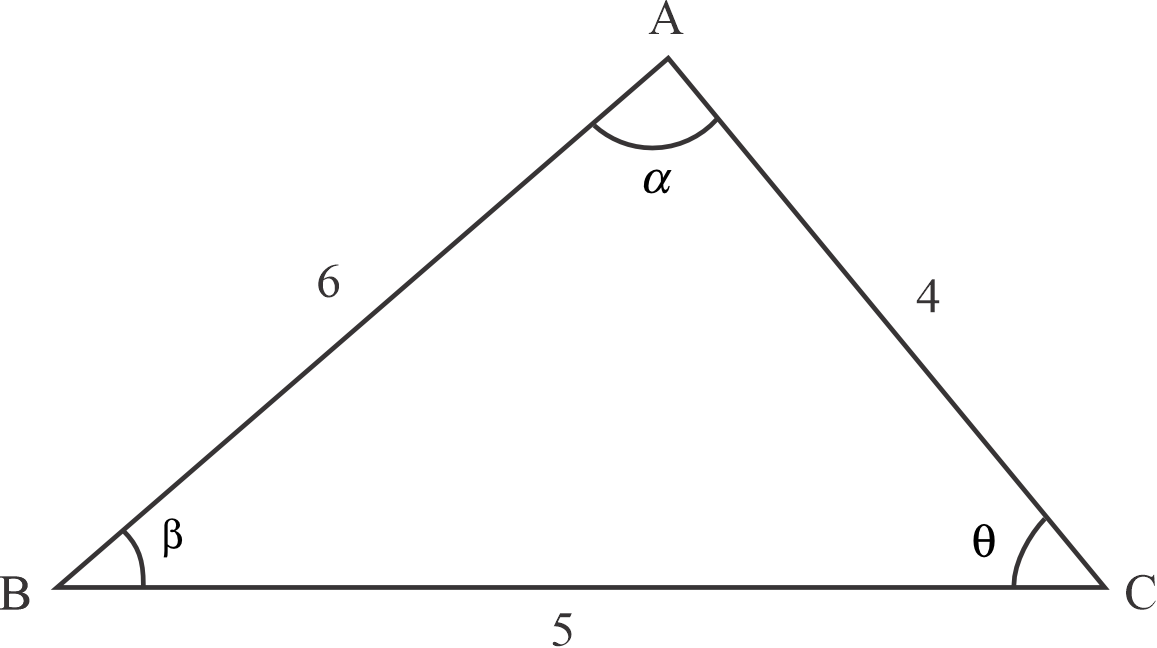
\includegraphics[width=0.8\textwidth]{imagenes/general2024-I/etapa1/bio/trigonometria3soluciong24-I}
	\end{minipage}
	
	
	
	
\end{enumerate}



\subsection*{Física}

\begin{enumerate}[resume]
	
	\item La figura muestra un cubo de arista $x$. Determine módulo de la resultante de los vectores  $\vec{R_1}$ y $\vec{R_2}$.
	
	
	\begin{figure}[h]
		\centering
		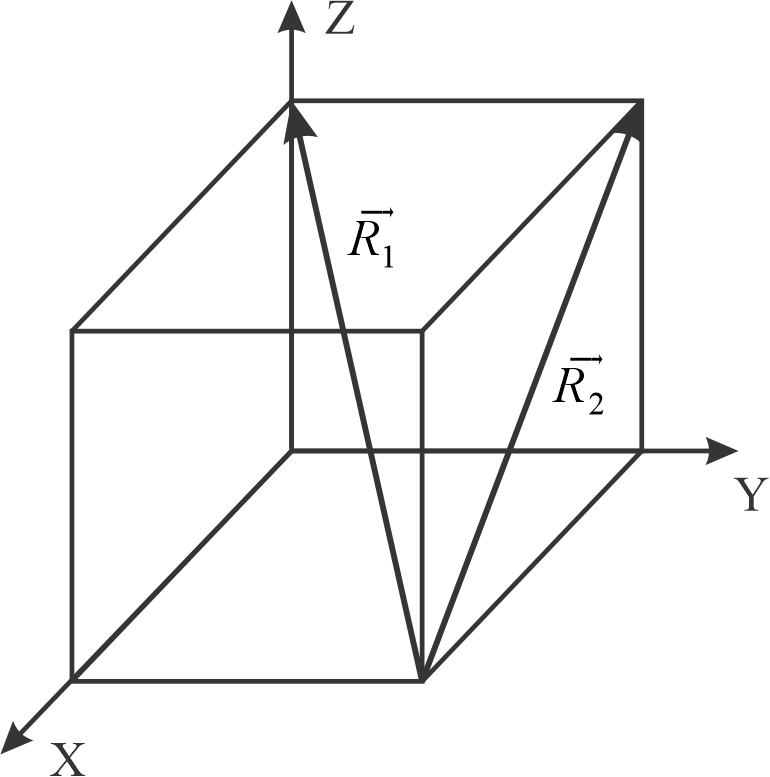
\includegraphics[width=0.3\textwidth]{imagenes/general2024-I/etapa1/bio/fisica1g24-I}
		%\caption{Descripción de la imagen}
		%\label{fig:ejemplo}
	\end{figure}
	
	
	
	\begin{enumerate}[label=\alph*)]
		\item $4x$
		\item $\,\,\,x$
		\item $2x$
		\item $3x$
		\item $5x$
	\end{enumerate}
	
	
	
	
	%\begin{tikzpicture}[overlay, remember picture]
	%	\node at (11, 3) %{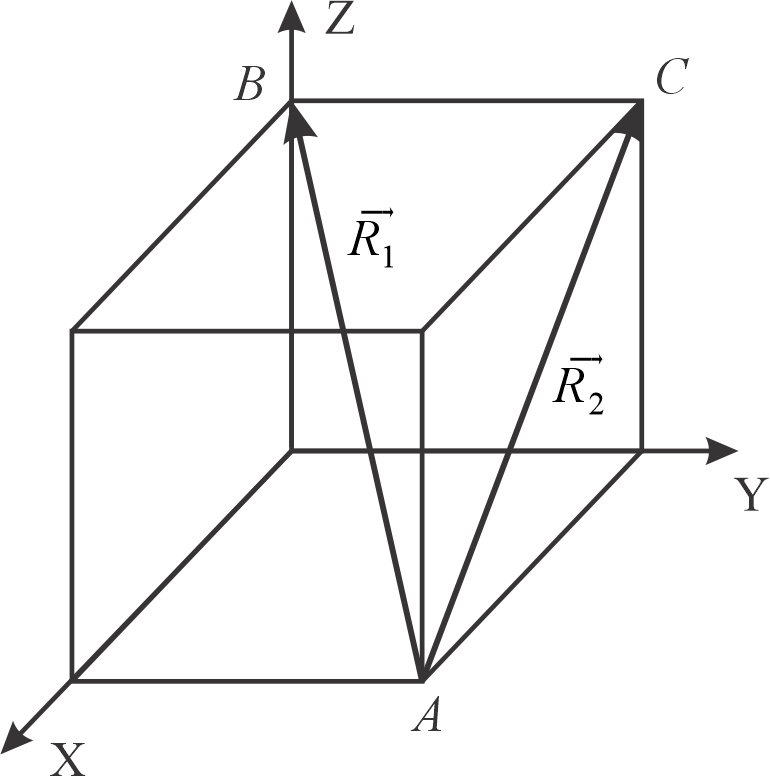
\includegraphics[width=0.4\textwidth]{BIO_PREG1_FISICA_SOLUCION}};
	%\end{tikzpicture}
	
	
	\textbf{Respuesta correcta:} d)
	
	\vspace{2mm}
	\textbf{Solucionario:}\\[1mm]
	
	
	
	
	%\AddToShipoutPicture*{\put(100,80){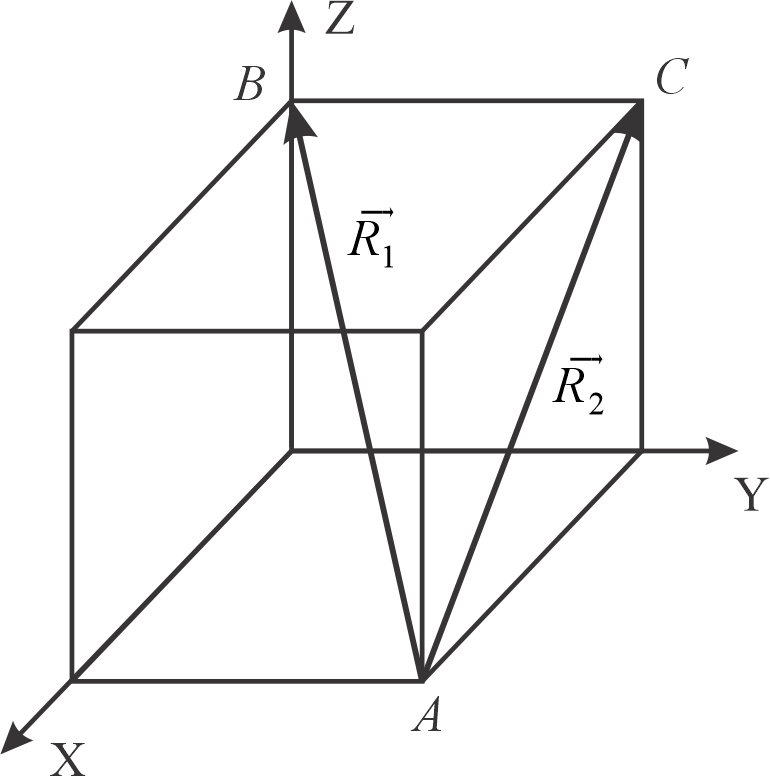
\includegraphics[scale=0.8]{BIO_PREG1_FISICA_SOLUCION}}} % Image background
	
	
	%\begin{figure}[h]
	%	\centering
	%	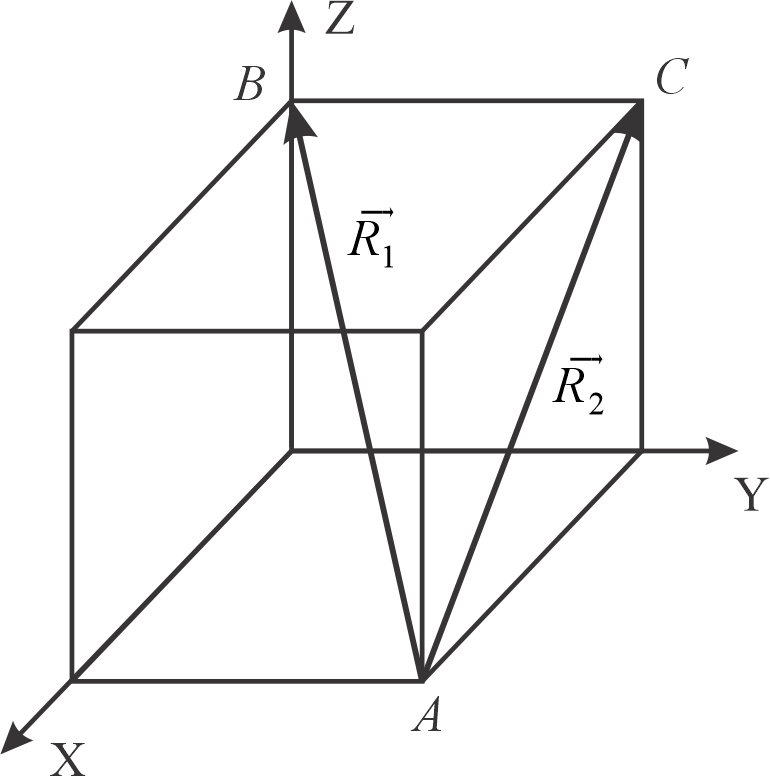
\includegraphics[width=0.4\textwidth]{BIO_PREG1_FISICA_SOLUCION}
	%\AddToShipoutPicture*{\put(100,80){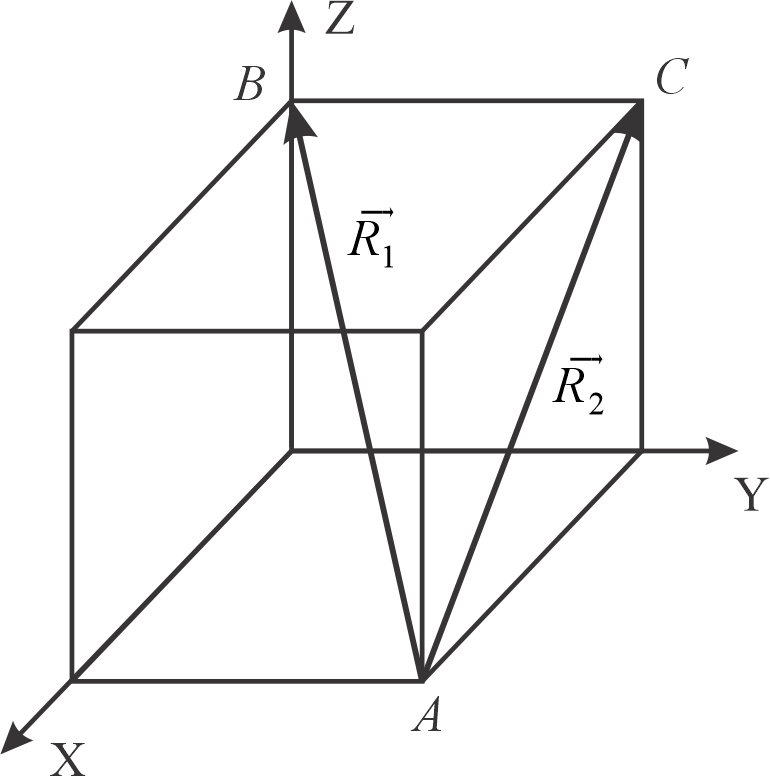
\includegraphics[scale=0.8]{BIO_PREG1_FISICA_SOLUCION}}} % Image background
	%\caption{Descripción de la imagen}
	%\label{fig:ejemplo}
	%\end{figure}
	
	
	De la figura:
	
	$A = (x,x,0)\\
	B = (0,0,x)\\
	C = (0,x,x)$\\
	
	
	$\overrightarrow {{R_{1}}}  = \overrightarrow {AB}  = B - A = (0,0,x) - (x,x,0)\\
	\overrightarrow {{R_{1}}}  = ( - x, - x,x)$
	
	\noindent
	\begin{minipage}[t]{0.5\textwidth}
		\vspace{2pt}
		$\overrightarrow {{R_{2}}}  = \overrightarrow {AC}  = C - A = (0,x,x) - (x,x,0)\\
		\overrightarrow {{R_{2}}}  = ( - x,0,x)\\
		\\$
		
		$\overrightarrow R  = \overrightarrow {{R_{1}}}  + \overrightarrow {{R_{2}}} \\
		\overrightarrow R  = ( - x, - x,x) + ( - x,0,x)\\
		\overrightarrow R  = ( - 2x, - x,2x)$
		
		$\left| {\overrightarrow R } \right| = \sqrt {{{( - 2x)}^2} + {{( - x)}^2} + {{(2x)}^2}}\\\\
		\left| {\overrightarrow R } \right| = \sqrt {{{4x}^2} + {{x}^2} + {{4x}^2}}\\
		\left| {\overrightarrow R } \right| = \sqrt {{{9x}^2}}=3x$	
		
	\end{minipage}
	\hfill
	\begin{minipage}[t]{0.5\textwidth}
		\vspace{0pt}
		\centering
		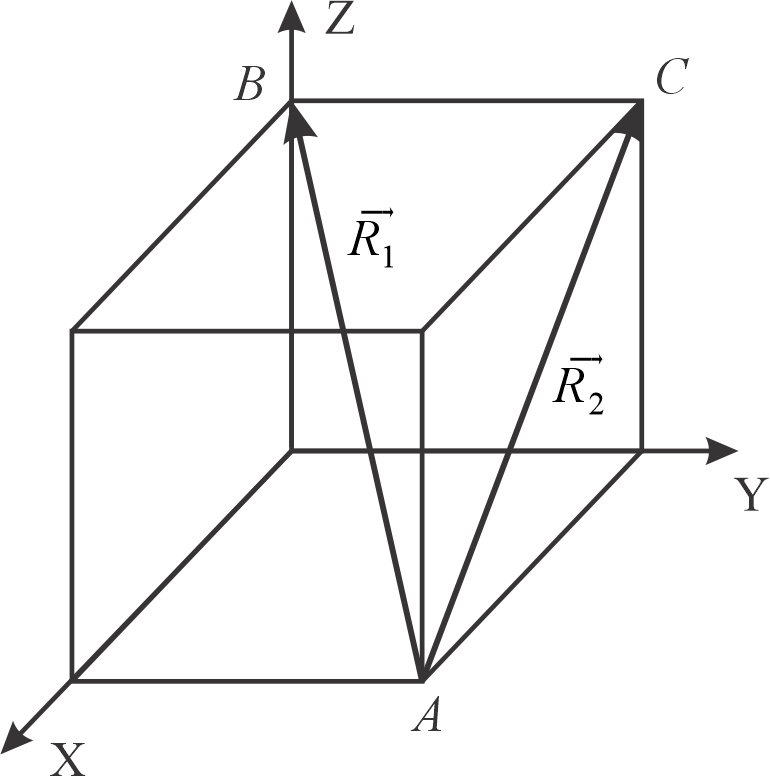
\includegraphics[width=0.68\textwidth]{imagenes/general2024-I/etapa1/bio/fisica1soluciong24-I}
	\end{minipage}
	
	
\end{enumerate}




\begin{enumerate}[resume]
	
	\item Un cuerpo esférico se lanza contra la pared, como se muestra en la figura. Si luego del impacto su rapidez disminuye en $1/3$, determine la relación entre la energía cinética antes y después del impacto. 
	
	
	\begin{figure}[h]
		\centering
		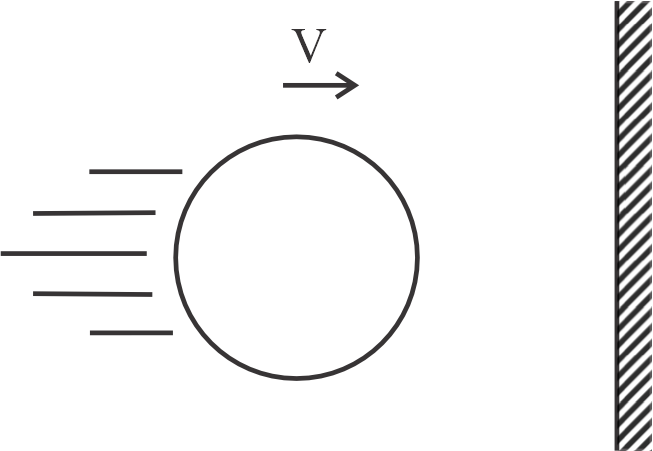
\includegraphics[width=0.3\textwidth]{imagenes/general2024-I/etapa1/bio/fisica2g24-I}
		%\caption{Descripción de la imagen}
		%\label{fig:ejemplo}
	\end{figure}
	
	
	
	\begin{enumerate}[label=\alph*)]
		\item $9/2$
		\item $9/4$
		\item $9/5$
		\item $\,\,\,\,\,9$
		\item $\,\,\,\,\,4$
	\end{enumerate}
	
	\textbf{Respuesta correcta:} b)
	
	\vspace{2mm}
	\textbf{Solucionario:}\\[1mm]
	
	
	$E_{c}\,\text{antes}=\dfrac{1}{2}mv^2\\$
	
	$E_{c}\,\text{después}=\dfrac{1}{2}m({{\dfrac{3}{3}v-\dfrac{1}{3}v}})^2\\\\$
	$E_{c}\,\text{después}=\dfrac{1}{2}m({\dfrac{2}{3}v})^2\\\\$
	$E_{c}\,\text{después}=\dfrac{1}{2}m{\dfrac{4}{2}v}^2=\dfrac{2}{9}mv^2\\$
	
	$\dfrac{{{E_c}\,\text{antes}}}{{{E_c}\,\text{después}}} = \dfrac{{\dfrac{1}{2}m{v^2}}}{{\dfrac{2}{9}m{v^2}}} = \dfrac{9}{4}$
	
	
\end{enumerate}



\begin{enumerate}[resume]
	
	\item Se tiene un alambre largo y delgado por el cual fluye una corriente de $20$ A. ¿A qué distancia del conductor la magnitud del campo magnético es $5\times10^{-4}T$? 
	\newline
	$\mu_o=4\pi\times10^{-7}\,\dfrac{Tm}{\text{A}}$  
	
	
	\begin{enumerate}[label=\alph*)]
		\item $0,4$ cm
		\item $0,5$ cm
		\item $0,6$ cm
		\item $0,7$ cm
		\item $0,8$ cm
	\end{enumerate}
	
	\textbf{Respuesta correcta:} e)
	
	\vspace{2mm}
	
	\noindent
	\begin{minipage}[t]{0.3\textwidth}
		\vspace{2pt}
		\textbf{Solucionario:}\\[1mm]
		
		$B = \dfrac{{{\mu_o}i}}{{2\pi x}}\\\\
		x = \dfrac{{{\mu_o}i}}{{2\pi B}}\\\\
		x = \dfrac{{4\pi  \times {{10}^{ - 7}}\dfrac{{Tm}}{A}(20A)}}{{2\pi (5\times {{10}^{ - 4}}T)}}\\
		x = \dfrac{{4\times {{10}^{ - 6}}}}{{5\times{{10}^{ - 4}}}} = \dfrac{4}{5}\times{10^{ - 2}}m\\\\
		x = 0,8\,cm$
		
	\end{minipage}
	\hfill
	\begin{minipage}[t]{0.7\textwidth}
		\vspace{0pt}
		\centering
		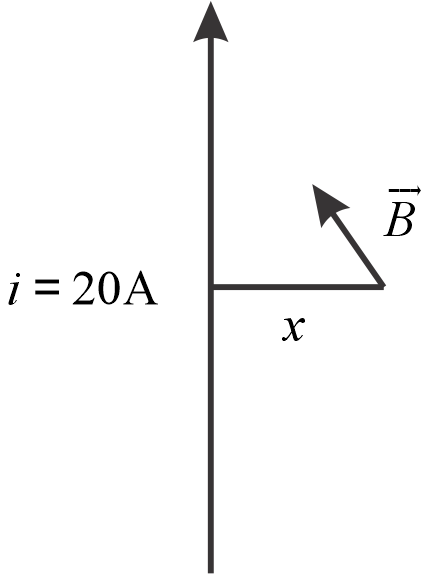
\includegraphics[width=0.3\textwidth]{imagenes/general2024-I/etapa1/bio/fisica3soluciong24-I}
	\end{minipage}
	
	
\end{enumerate}



\subsection*{Química}

\begin{enumerate}[resume]
	
	\item ¿Cuál es la normalidad de una solución que contiene $50$g de ácido sulfúrico en $500$mL de solución?
	\newline
	$(\text{H}=1;\,\text{S}=32;\,\text{O}=16)$
	
	\begin{enumerate}[label=\alph*)]
		\item $2,00$
		\item $2,08$
		\item $2,04$
		\item $2,40$
		\item $2,50$
	\end{enumerate}
	
	\textbf{Respuesta correcta:} c)
	
	\vspace{2mm}
	\textbf{Solucionario:}\\[1mm]
	
	Datos: (H$_2$SO$_4$)
	
	$\text{H}=1\times2\,\,\,=2\\
	\text{S}\,=32\times1=32\\
	\text{O}=16\times4=64$
	
	$\,\,\,\,\,\,\,\,\,\,\,\,\,\,\,\,\,\,\,\,\,\,\,\,\,\,\,\,\,\,=\overline {{\rm{98 g/mol}}}\\$
	
	Volumen solución $=500\text{ml}=0.5\text{L}\\$
	Gramos de soluto $=50\text{g}$\\
	
	Hallando el número equivalente gramo de un ácido:
	
	${\rm{Eq}} - {\rm{g}} = \dfrac{{{\rm{gr}}\,{\rm{soluto}}}}{{{\rm{\# }}\,{\rm{Equivalente}}\,{\rm{gramo}}\,{\rm{\text{ácido}}}\,{\rm{(H)}}}}\\\\
	{\rm{Eq}} - {\rm{g}}\,\,{\rm{\text{ácido}}}\, = \dfrac{{{\rm{gr}}\,{\rm{soluto}}}}{{{\rm{\# }}\,{\rm{Equivalente}}\,{\rm{gramo}}\,{\rm{\text{ácido}}}\,{\rm{(H)}}}}\\\\
	{\rm{Eq}} - {\rm{g}}\,\,{\rm{\text{ácido}}}\,{\rm{\text{sulfúrico}}} = \,49\,{\rm{g}}$\\
	
	Hallando el número equivalente:\\
	${\rm{Eq}} - {\rm{g}} = \dfrac{{50\,{\rm{g}}}}{{49\,{\rm{g}}}} = 1,02\,{\rm{g}}$
	
	Hallando la normalidad:\\
	
	${\rm{N = }}\dfrac{{{\rm{N^\circ  Eq}} - {\rm{g}}}}{{{\rm{U}}\,{\rm{\text{solución}}}}}\\\\
	{\rm{N = }}\dfrac{{1,02}}{{{\rm{0,5}}}}\\\\
	{\rm{N = 2,04}}$
	
	
	
\end{enumerate}


\begin{enumerate}[resume]
	
	\item En la relación a la ecuación química, indique verdadero (V) O (F) según corresponda.
	\[HC{I_{(ac)}} + NaO{H_{(ac)}} \to {H_2}{O_{(l)}} + calor\]
	
	\begin{enumerate}[label=\Roman*.]
		\item Es una reacción de metátesis.
		\item Es una reacción exotérmica.
		\item Es una reacción de simple desplazamiento.
	\end{enumerate}
	
	
	\begin{enumerate}[label=\alph*)]
		\item VVV
		\item FVF
		\item FVV
		\item VVF
		\item FFV
	\end{enumerate}
	
	\textbf{Respuesta correcta:} d)
	
	\vspace{2mm}
	\textbf{Solucionario:}\\[1mm]
	
	
	\begin{enumerate}[label=\Roman*.]
		\item ${\rm{Verdadero}} \to \text{Posee la forma}\,\,\,\,\,\,\,\,{\rm{AB}} + {\rm{CD}} \to {\rm{AC}} + {\rm{BD}}\\
		{\rm{   }} \Rightarrow {\text{corresponde a una reacción de metátesis. }}$
		
		\item ${\rm{Verdadero}} \to \text{Como la reacción genera calor}\\
		{\rm{   }} \Rightarrow {\text{es una reacción exotérmica. }}$
		
		\item ${\rm{Falso}} \to \text{Al ser una reacción de metátesis se desarrolla doble desplazamiento.}$\\
		
	\end{enumerate}
	
\end{enumerate}


\begin{enumerate}[resume]
	
	\item Se necesitan $200$ calorías para que $500$g de un cuerpo eleve su temperatura desde $20^\circ$C hasta $25^\circ$C. Determine el peso atómico de este cuerpo. 
	\begin{enumerate}[label=\alph*)]
		\item $64,5$
		\item $78,7$
		\item $36,4$
		\item $86,5$
		\item $49,5$
	\end{enumerate}
	
	\textbf{Respuesta correcta:} b)
	
	\vspace{2mm}
	\textbf{Solucionario:}\\[1mm]
	
	Datos:\\
	$d=200\,cal$\\
	$m=500 \rm{g}$\\
	$\bigtriangleup T=25-20=5^\circ C$
	
	Según la ley de Dulong y Petit:\\
	$PA \times CE = 6,3\\
	PA = \dfrac{{6,3}}{{CE}}$\\
	
	$d=m\times CE\times \bigtriangleup T\\\\
	CE = \dfrac{{d}}{{m\times \bigtriangleup T}}\\\\
	CE = \dfrac{{200\,cal}}{{500 \rm{g}\times 20^\circ C}}=\dfrac{2}{25}$\\\\
	
	Reemplazando:\\\\
	$PA = \dfrac{{6,3}}{{2/25}} = \dfrac{{25 \times 6,3}}{2} = 25 \times 3,15\\\\
	\boxed{{\therefore PA = 78,7}}$
	
	
\end{enumerate}


\begin{enumerate}[resume]
	
	\item ¿Qué procesos no están relacionados con la electrólisis?
	
	\begin{enumerate}[label=\Roman*.]
		\item La producción de energía eléctrica
		\item La producción de metales con una fina capa de otro metal
		\item La descarga de la batería en los teléfonos móviles
		\item La síntesis de elementos 
		
	\end{enumerate}
	
	
	\begin{enumerate}[label=\alph*)]
		\item Sólo II
		\item Sólo I
		\item Sólo IV
		\item I y III
		\item IV, II y III
	\end{enumerate}
	
	\textbf{Respuesta correcta:} d)
	
	\vspace{2mm}
	\textbf{Solucionario:}
	
	ELECTROLÍSIS\\
	Es un proceso no espontáneo en el cual, por acción de la energía eléctrica que proviene de una fuente de voltaje, se logra desarrollar reacciones REDOX. Se realiza en un medio acuoso. Por lo tanto la producción de energía eléctrica y la descarga de la batería en los teléfonos móviles, no se realiza en medio acuoso.
	
	
\end{enumerate}


\begin{enumerate}[resume]
	
	\item Un gas está confinado en un cilindro de acero de $10,0$ litros, a un apresión de 5 atmósferas y a $27^\circ$C. Si la temperatura se eleva a  $327^\circ$C. ¿Cuál será la presión del gas (en atm) en el interior del cilindro?
	
	\begin{enumerate}[label=\alph*)]
		\item $\,\,\,1,5$
		\item $10,0$
		\item $\,\,\,7,5$
		\item $12,5$
		\item $15,0$
	\end{enumerate}
	
	\textbf{Respuesta correcta:} b)
	
	\vspace{2mm}
	\textbf{Solucionario:}\\[1mm]
	
	
	%\iffalse
	\begin{minipage}[t]{0.45\textwidth}
		Datos:\\
		$V = 10\,L\\
		{P_{\,1}} = 5\,atm\\
		{T_{\,1}} = 27^\circ \rm{C}\\
		{T_{\,2}} = 327^\circ \rm{C}\\
		{P_{\,2}} = ?$
	\end{minipage}
	\hfill
	\begin{minipage}[t]{0.45\textwidth}
		$\dfrac{{{P_{\,1}}}}{{{T_{\,1}}}} = \dfrac{{{P_{\,2}}}}{{{T_{\,2}}}}\\\\
		{P_{\,2}} = \dfrac{{{T_{\,2}}}}{{{T_{\,1}}}}{P_{\,1}}\\\\
		{P_{\,2}} = \dfrac{{327^\circ \rm{C} + 273}}{{27^\circ \rm{C} + 273}}(5\,atm)\\\\
		{P_{\,2}} = \dfrac{{600}}{{300}}(5\,atm)\\\\
		\boxed{{P_{\,2}} = 10\,atm}$
	\end{minipage}
	%\fi
\end{enumerate}

\subsection*{Biología y Anatomía}

\begin{enumerate}[resume]
	
	\item Este parásito es el agente causal de la oxiurasis, se presenta principalmente en grupos familiares e institucionales (guarderías, jardines y escuelas).
	
	\begin{enumerate}[label=\alph*)]
		\item \textit{Enterobius vermicularis}
		\item \textit{Acaris lumbricoides}
		\item \textit{Entamoeba histolytica}
		\item \textit{Fasciola hepática}
		\item \textit{Echinococcus granulosus}
	\end{enumerate}
	
	\textbf{Respuesta correcta:} a)
	
	\vspace{2mm}
	\textbf{Solucionario:}
	
	La oxiurasis o enterobiasis es una parasitosis intestinal producida por \textit{Enterobius vermicularis}, conocido también como oxiuro. Se transmite con facilidad en grupos familiares y escolares por contacto directo o por objetos contaminados. Por ello, la alternativa correcta es \textit{Enterobius vermicularis}.
	
\end{enumerate}


\begin{enumerate}[resume]
	
	\item ¿Cuál es la anomalía cromosómica en la que los testículos se degeneran lentamente y conducen al crecimiento mamario?
	
	\begin{enumerate}[label=\alph*)]
		\item Síndrome de Edwards
		\item Síndrome de Down
		\item Síndrome de Patau 
		\item Síndrome de Klinefelter
		\item Síndrome de Turner
	\end{enumerate}
	
	\textbf{Respuesta correcta:} d)
	
	\vspace{2mm}
	\textbf{Solucionario:}
	
	El síndrome de Klinefelter se presenta en varones con cariotipo 47,XXY. Entre sus características destacan hipogonadismo, degeneración testicular progresiva y ginecomastia (crecimiento mamario). Por eso, la respuesta correcta es síndrome de Klinefelter.
	
\end{enumerate}

\begin{enumerate}[resume]
	
	\item ¿Qué estructura se encuentra exactamente en donde empieza la uretra membranosa?
	
	\begin{enumerate}[label=\alph*)]
		\item próstata
		\item gládula de Cowper
		\item vesísulas seminales 
		\item glándulas de Leydig
		\item glándulas de Skene
	\end{enumerate}
	
	\textbf{Respuesta correcta:} b)
	
	\vspace{2mm}
	\textbf{Solucionario:}
	
	La uretra membranosa se inicia al salir de la próstata y en esa región se relaciona con las glándulas bulbouretrales o glándulas de Cowper. Estas secretan una sustancia lubricante antes de la eyaculación. Por ello, la alternativa correcta es glándula de Cowper.
	
\end{enumerate}


\begin{enumerate}[resume]
	
	\item Durante la profase I de la meiosis, en uno de los periodos, los cromosomas bivalentes alcanzan su estado máximo de condensación, ocurriendo una reducción en el número de quiasmas. Este proceso corresponde a:
	
	\begin{enumerate}[label=\alph*)]
		\item Paquinema 
		\item Diplonema
		\item Cigonema
		\item Diacinesis
		\item Leptonema
	\end{enumerate}
	
	\textbf{Respuesta correcta:} d)
	
	\vspace{2mm}
	\textbf{Solucionario:}
	
	En la diacinesis, etapa final de la profase I, los cromosomas alcanzan su máxima condensación y los quiasmas disminuyen por terminalización. Esa es la característica descrita en el enunciado. Por lo tanto, la respuesta correcta es diacinesis.
	
\end{enumerate}

\begin{enumerate}[resume]
	
	\item ¿Cuál es la asociación interespecífica en la que una de las especies, debido a su desarrollo y producción de sustancias inhibidoras, impide el crecimiento de la otra especie?
	
	\begin{enumerate}[label=\alph*)]
		\item Protocooperación
		\item Amensalismo
		\item Inquilinismo
		\item Comensalismo
		\item Parasitismo
	\end{enumerate}
	
	\textbf{Respuesta correcta:} b)
	
	\vspace{2mm}
	\textbf{Solucionario:}
	
	El amensalismo es una relación interespecífica donde una especie resulta perjudicada y la otra no obtiene beneficio ni daño. Esto ocurre, por ejemplo, cuando una especie libera sustancias inhibidoras que impiden el crecimiento de otra. Por eso, la respuesta es amensalismo.
	
\end{enumerate}


\begin{enumerate}[resume]
	
	\item ¿Cuáles son las células del sistema inmunitario capaces de detectar cambios en las características de algunas células propias que han sido infectadas por virus o que se han degenerado convirtiéndose en células tumorales?
	
	\begin{enumerate}[label=\alph*)]
		\item Linfocitos supresores.
		\item Linfocitos B.
		\item Linfocitos "Helper".
		\item Linfocitos NK.
		\item Linfocitos polimorfonucleares.
	\end{enumerate}
	
	\textbf{Respuesta correcta:} d)
	
	\vspace{2mm}
	\textbf{Solucionario:}
	
	Los linfocitos NK (Natural Killer) reconocen y destruyen células infectadas por virus y células tumorales sin necesidad de una sensibilización previa específica. Su función principal es la vigilancia inmunológica. Por ello, la respuesta correcta es linfocitos NK.
	
\end{enumerate}

\subsection*{Psicología y Filosofía}

\begin{enumerate}[resume]
	
	\item Juana recuerda una imagen que vió en el parque de diversiones. Esta información preliminar específica del cerebro corresponde a:
	
	\begin{enumerate}[label=\alph*)]
		\item el hipotálamo.
		\item el cerebelo.
		\item el tálamo.
		\item el hemisferio izquierdo.
		\item el hemisferio derecho.
	\end{enumerate}
	
	\textbf{Respuesta correcta:} c)
	
	\vspace{2mm}
	\textbf{Solucionario:}
	
	El tálamo actúa como centro de relevo sensorial, organizando e integrando información que luego será procesada por la corteza cerebral. Por ello, ante una información preliminar relacionada con imágenes, la estructura señalada es el tálamo.
	
\end{enumerate}

\begin{enumerate}[resume]
	
	\item Pedro escoge su carrera no porque sea la que más le agrade, sino porque le va proporcionar mayores satisfacciones económicas. ¿Qué actitud asumió Pedro?
	
	\begin{enumerate}[label=\alph*)]
		\item Pragmática
		\item Religiosa
		\item Moral
		\item Definitoria
		\item Problematizadora
	\end{enumerate}
	
	\textbf{Respuesta correcta:} a)
	
	\vspace{2mm}
	\textbf{Solucionario:}
	
	La actitud pragmática se caracteriza por valorar principalmente la utilidad o conveniencia práctica de una decisión. Pedro elige la carrera por el beneficio económico y no por gusto personal. Por eso, la respuesta correcta es pragmática.
	
\end{enumerate}


\begin{enumerate}[resume]
	
	\item Le encanta la compañía, pero aveces busca la soledad; ama profundamente, aveces se desilusiona, lucha y muestra tenacidad por lo que parece su meta, para después decaer y perder el interés.\\\\
	Estas son características de inndividuos que se hallan en la:
	
	
	\begin{enumerate}[label=\alph*)]
		\item senectud.
		\item juventud.
		\item infancia.
		\item adolescencia.
		\item niñez.
	\end{enumerate}
	
	\textbf{Respuesta correcta:} d)
	
	\vspace{2mm}
	\textbf{Solucionario:}
	
	La adolescencia se caracteriza por cambios emocionales intensos, inestabilidad afectiva, contradicciones conductuales y búsqueda de identidad. Las descripciones del enunciado corresponden a esa etapa del desarrollo. Por lo tanto, la respuesta correcta es adolescencia.
	
\end{enumerate}



\begin{enumerate}[resume]
	
	\item \textit{La tierra gira alrededor del sol.}\\\\
	Este enunciado es aceptado por toda la comunidad de individuos cognoscentes en el planeta corresponde al conocimiento:
	
	
	\begin{enumerate}[label=\alph*)]
		\item objetivo.
		\item universal.
		\item necesario.
		\item fundamentado.
		\item racional.
	\end{enumerate}
	
	\textbf{Respuesta correcta:} b)
	
	\vspace{2mm}
	\textbf{Solucionario:}
	
	Un conocimiento es universal cuando su validez es aceptada por todos o tiene alcance general para todos los sujetos cognoscentes. El enunciado dado es reconocido por la comunidad científica y por la humanidad en general. Por eso, corresponde al conocimiento universal.
	
\end{enumerate}


\subsection*{Geografía}

\begin{enumerate}[resume]
	
	\item En el sistema hidrográfico del Perú, la cuenca endorreica corresponde a la vertiente del:
	
	
	\begin{enumerate}[label=\alph*)]
		\item Atlántico.
		\item Pacífico.
		\item Titicaca.
		\item Amazonas.
		\item Marañon.
	\end{enumerate}
	
	\textbf{Respuesta correcta:} c)
	
	\vspace{2mm}
	\textbf{Solucionario:}
	
	Las cuencas endorreicas son aquellas cuyas aguas no desembocan en el mar, sino en lagos interiores. En el Perú, la vertiente endorreica corresponde al lago Titicaca. Por ello, la respuesta correcta es Titicaca.
	
\end{enumerate}

\begin{enumerate}[resume]
	
	\item Los aspectos fundamentales de la biodiversidad son: la variedad genética, la diversidad de especies y la ...
	
	\begin{enumerate}[label=\alph*)]
		\item diversidad de ecosistemas.
		\item megadiversidad.
		\item ecología y desarrollo sotenible.
		\item diversidad botánica.
		\item diversidad zoológica.
	\end{enumerate}
	
	\textbf{Respuesta correcta:} a)
	
	\vspace{2mm}
	\textbf{Solucionario:}
	
	La biodiversidad comprende tres niveles fundamentales: diversidad genética, diversidad de especies y diversidad de ecosistemas. Esta última considera la variedad de hábitats y comunidades ecológicas. Por eso, la respuesta correcta es diversidad de ecosistemas.
	
\end{enumerate}



\subsection*{Historia}

\begin{enumerate}[resume]
	
	\item Entre 1347 y 1353, se produjo la pandemia más mortífera dela historia, conocida como $\_\_\_\_\_\_\_\_\_$. Los síntomas eran fiebre alta, dolores musculares, tos persistente. gangrena en dedos de las extremidades y aparición de enormes ampollas.
	
	\begin{enumerate}[label=\alph*)]
		\item tifoidea
		\item malaria
		\item peste negra
		\item cólera 
		\item peste amarilla
	\end{enumerate}
	
	\textbf{Respuesta correcta:} c)
	
	\vspace{2mm}
	\textbf{Solucionario:}
	
	La pandemia que asoló Europa entre 1347 y 1353 fue la peste negra, una de las más mortíferas de la historia. Produjo millones de muertes y se asoció a bubones, fiebre alta y gangrena. Por ello, la respuesta correcta es peste negra.
	
\end{enumerate}

\begin{enumerate}[resume]
	
	\item En 1856, el Dr. Cayetano Heredia impulsó la creación de la $\_\_\_\_\_\_\_\_\_\_\_$, como ente encargado del entrenamiento y vigilancia de la profesión médica.
	
	\begin{enumerate}[label=\alph*)]
		\item Facultad de Medicina del Perú
		\item Facultad de Medicina del Lima
		\item Facultad de Medicina del San Marcos
		\item Escuela Médica del Perú
		\item Universidad Mayor de San Marcos
		
	\end{enumerate}
	
	\textbf{Respuesta correcta:} b)
	
	\vspace{2mm}
	\textbf{Solucionario:}
	
	La pregunta alude a la reorganización de la enseñanza médica impulsada por Cayetano Heredia en el siglo XIX. Según la clave marcada, la respuesta correcta es Facultad de Medicina de Lima, institución destinada al entrenamiento y vigilancia de la profesión médica.
	
\end{enumerate}


\subsection*{Educación Cívica}


\begin{enumerate}[resume]
	
	\item El Congreso puede delegar al Poder Ejecutivo la facultad de legislar mediante:
	
	\begin{enumerate}[label=\alph*)]
		\item Decreto de Urgencia
		\item Decreto Supremo
		\item Decreto Legislativo
		\item Decreto Ley
		\item Edicto Municipal
	\end{enumerate}
	
	\textbf{Respuesta correcta:} c)
	
	\vspace{2mm}
	\textbf{Solucionario:}
	
	Cuando el Congreso delega facultades legislativas al Poder Ejecutivo, este emite decretos legislativos. Estos tienen rango de ley y se dictan dentro del marco y plazo establecidos por el Congreso. Por lo tanto, la respuesta correcta es Decreto Legislativo.
	
\end{enumerate}

\begin{enumerate}[resume]
	
	\item En el Perú, la entidad autónoma encragada de supervisar la legalidad de la ejecución del presupuesto del Estado es:
	
	\begin{enumerate}[label=\alph*)]
		\item Contraloría General de la República.
		\item Banco Central de Reserva del Perú.
		\item Superintendencia de Banca y Seguros.
		\item Consejo Nacional de la Magistratura.
		\item Jurado Nacional de Elecciones.
	\end{enumerate}
	
	\textbf{Respuesta correcta:} a)
	
	\vspace{2mm}
	\textbf{Solucionario:}
	
	La Contraloría General de la República es el órgano superior del Sistema Nacional de Control. Su función es supervisar la legalidad de la ejecución del presupuesto público y el uso de los recursos del Estado. Por eso, la respuesta correcta es Contraloría General de la República.
	
\end{enumerate}


\subsection*{Economía}

\begin{enumerate}[resume]
	
	\item El creciente desempleo y subempleo en nuestra economía, durante los últimos años, han originado principalmente:
	
	\begin{enumerate}[label=\alph*)]
		\item una mayor apertura de mercados formales.
		\item el incremento de mercados informales.
		\item mayores niveles de ahorro.
		\item un mayor acceso a los mercados cerrados.
		\item un mayor consumo de las familias.
	\end{enumerate}
	
	\textbf{Respuesta correcta:} b)
	
	\vspace{2mm}
	\textbf{Solucionario:}
	
	Cuando aumentan el desempleo y el subempleo, muchas personas recurren a actividades económicas no reguladas para generar ingresos. Eso produce el crecimiento de la informalidad. Por lo tanto, la respuesta correcta es el incremento de mercados informales.
	
\end{enumerate}

\begin{enumerate}[resume]
	
	\item Según los teóricos neoliberales, el Estado debe participar en la economía en la medida en que exista:
	
	\begin{enumerate}[label=\alph*)]
		\item barreras de mercado.
		\item fallas de mercado.
		\item políticas económicas.
		\item posiciones dominantes de mercado.
		\item económias a escala.
	\end{enumerate}
	
	\textbf{Respuesta correcta:} b)
	
	\vspace{2mm}
	\textbf{Solucionario:}
	
	Desde la perspectiva neoliberal, la intervención del Estado debe ser limitada y justificarse principalmente cuando el mercado no asigna eficientemente los recursos. Estas situaciones se denominan fallas de mercado. Por ello, la respuesta correcta es fallas de mercado.
	
\end{enumerate}



\subsection*{Comunicación}

\begin{enumerate}[resume]
	
	\item Consiste en escribir de manera breve y precisa los puntos más resaltantes de un texto en el proceso de la lectura.
	
	\begin{enumerate}[label=\alph*)]
		\item El resumen
		\item Las notas al margen
		\item El esquema
		\item La síntesis
		\item El sumillado
	\end{enumerate}
	
	\textbf{Respuesta correcta:} b)
	
	\vspace{2mm}
	\textbf{Solucionario:}
	
	Las notas al margen consisten en escribir breves apuntes o ideas clave al costado del texto mientras se lee. Sirven para destacar lo más importante de manera precisa y rápida. Por eso, la respuesta correcta es las notas al margen.
	
\end{enumerate}

\begin{enumerate}[resume]
	
	\item La anemia es la disminución de las células rojas de la sangre.\\
	El propósito comunicativo del texto es:
	
	\begin{enumerate}[label=\alph*)]
		\item convencer.
		\item deleitar.
		\item informar.
		\item instruir.
		\item advertir.
	\end{enumerate}
	
	\textbf{Respuesta correcta:} c)
	
	\vspace{2mm}
	\textbf{Solucionario:}
	
	El enunciado brinda una definición objetiva sobre la anemia. No intenta persuadir ni entretener, sino transmitir un dato. Por lo tanto, el propósito comunicativo es informar.
	
\end{enumerate}

\begin{enumerate}[resume]
	
	\item Pedro al culminar sus estudios en el área de Biomédicas, elaborará un documento para que el emitan su certificado de estudios.\\
	¿Qué documento presentar a la coordinación académica de su escuela profesional?
	
	\begin{enumerate}[label=\alph*)]
		\item Oficio
		\item Memorial
		\item Carta
		\item Informe
		\item Solicitud
	\end{enumerate}
	
	\textbf{Respuesta correcta:} e)
	
	\vspace{2mm}
	\textbf{Solucionario:}
	
	Cuando una persona pide formalmente un documento o trámite ante una institución, debe presentar una solicitud. En este caso, Pedro desea que le emitan su certificado de estudios. Por ello, la respuesta correcta es solicitud.
	
\end{enumerate}


\begin{enumerate}[resume]
	
	\item La función del lenguaje que expresa el mundo interior del sujeto es la:
	
	\begin{enumerate}[label=\alph*)]
		\item poética.
		\item metalinguística.
		\item apelativa.
		\item fática.
		\item expresiva.
	\end{enumerate}
	
	\textbf{Respuesta correcta:} e)
	
	\vspace{2mm}
	\textbf{Solucionario:}
	
	La función expresiva o emotiva del lenguaje manifiesta sentimientos, emociones, estados de ánimo y opiniones del hablante. Como el enunciado se refiere al mundo interior del sujeto, la respuesta correcta es expresiva.
	
\end{enumerate}


\subsection*{Literatura}

\begin{enumerate}[resume]
	
	\item ¿Qué figuras literarias están presentes en los versos?\\\\
	"Si eres muerte, ¿por qué me das la vida?\\ 
	si eres vida, ¿por qué me das la muerte?"
	
	\begin{enumerate}[label=\alph*)]
		\item Epítelo y simil
		\item Anáfora y metáfora
		\item Anáfora y paradoja
		\item Anáfora y antítesis
		\item Metáfora y retruécano
	\end{enumerate}
	
	\textbf{Respuesta correcta:} c)
	
	\vspace{2mm}
	\textbf{Solucionario:}
	
	Hay anáfora porque se repite la estructura inicial ``si eres...''. Además, existe paradoja porque se unen ideas aparentemente contradictorias: muerte que da vida y vida que da muerte. Por eso, la respuesta correcta es anáfora y paradoja.
	
\end{enumerate}

\begin{enumerate}[resume]
	
	\item ¿Cuál es el mensaje que evoca los versos del poema Heraldos Negros?\\\\
	Hay golpes en la vida tan fuertes ... ¡Yo no sé!\\
	golpes como el odio de Dios\\
	como si ante ello,\\
	la resaca de todo lo sufrido\\
	se empozara en el alma ... ¡Yo no sé!
	
	\begin{enumerate}[label=\alph*)]
		\item El poeta expresa en forma dolida el sufrimiento humano.
		\item El poeta expresa el odio al hombre.
		\item El poeta percibe el odio de Dios.
		\item El poeta percibe la incomprensión a las penurias del hombre.
		\item El poeta suspira y se congoja sin causa.
	\end{enumerate}
	
	\textbf{Respuesta correcta:} a)
	
	\vspace{2mm}
	\textbf{Solucionario:}
	
	En los versos de \textit{Los heraldos negros}, César Vallejo expresa el dolor profundo que causan ciertos golpes de la vida. El tema central es el sufrimiento humano ante experiencias dolorosas e inexplicables. Por ello, la respuesta correcta es la alternativa a).
	
\end{enumerate}

\subsection*{Razonamiento Matemático}

\begin{enumerate}[resume]
	
	\item Tres pasajeras se sientan alrededor de una mesa circular con 6 sillas distribuidas simétricamente. Se sabe que:
	
	\begin{itemize}[label=--]
		\item A la derecha de la novia de Alberto se sienta Gabriel.
		\item Mary, que está sentada a la derecha de Dora, está sentada al frente de su propio novio.
		\item Alberto está a la izquierda de Mario.
		\item Esperanza está al frente de la novia de Gabriel.
	\end{itemize}
	
	¿Quién es el novio de Dora?
	
	\begin{enumerate}[label=\alph*)]
		\item Antonio
		\item Gabriel
		\item Alberto
		\item Mario
		\item José
	\end{enumerate}
	
	\textbf{Respuesta correcta:} b)
	
	\vspace{2mm}
	\textbf{Solucionario:}\\
	
	Iniciando con el último dato.
	
	\noindent
	\begin{minipage}[t]{0.40\textwidth}
		\vspace{5pt}
		Del segundo dato, Mary está al frente de su propio novio, por tanto no puede ser Mary.
		
		Tampoco puede ser Esperanza, entonces la única posibilidad es que la novia de Gabriel sea Dora.
		
		$\therefore$ El novio de Dora es Gabriel.
	\end{minipage}
	\hfill
	\begin{minipage}[t]{0.35\textwidth}
		\vspace{0pt}
		\centering
		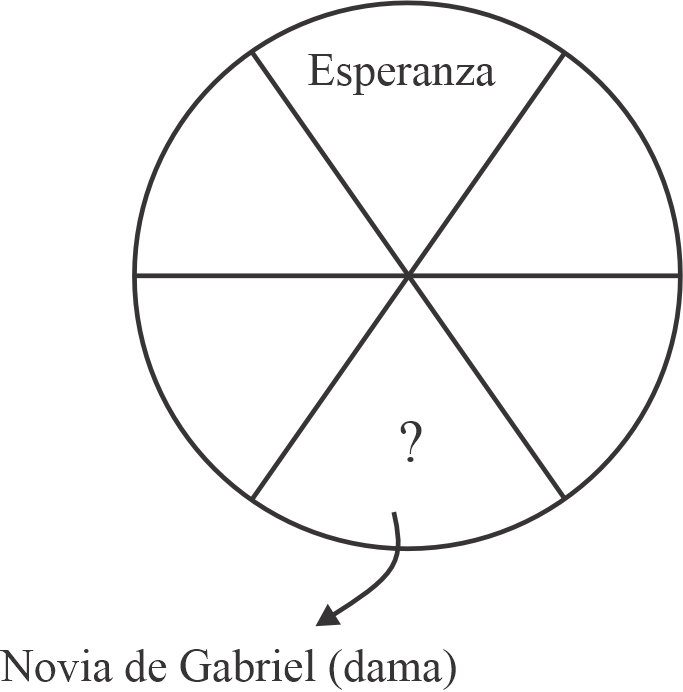
\includegraphics[width=4cm]{imagenes/general2024-I/etapa1/bio/razonamientomatematico1soluciong24-I}
	\end{minipage}
	
\end{enumerate}

\begin{enumerate}[resume]
	
	\item En un concierto hay tantas parejas bailando como varones parados. 300 damas no bailan, si las personas que no bailan son el triple de las damas que bailan, además hay 100 varones más bailando que sentados. ¿Cuántos varones bailan?
	
	\begin{enumerate}[label=\alph*)]
		\item $100$
		\item $150$
		\item $200$
		\item $150$
		\item $300$
	\end{enumerate}
	
	\textbf{Respuesta correcta:} c)
	
	\vspace{2mm}
	\textbf{Solucionario:}\\
	
	\begin{figure}[h]
		\centering
		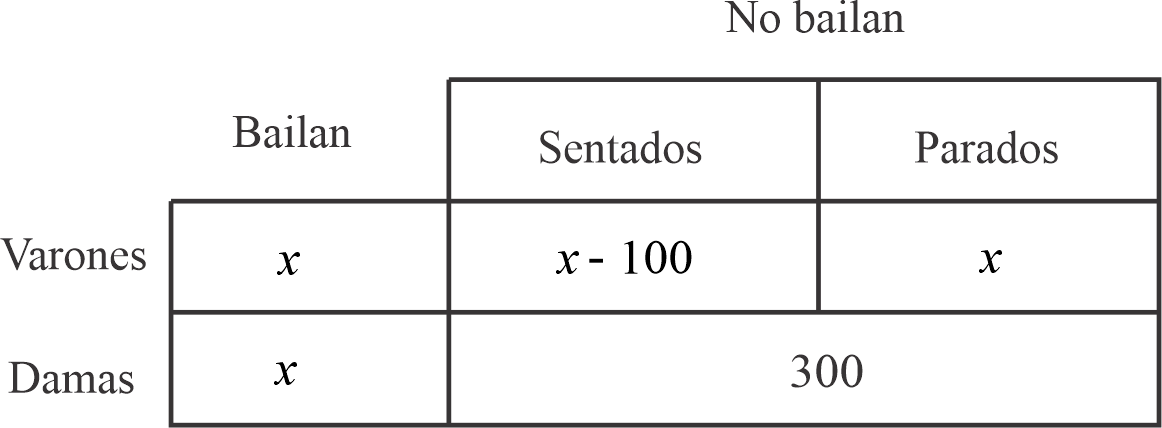
\includegraphics[width=5.5cm]{imagenes/general2024-I/etapa1/bio/razonamientomatematico2soluciong24-I}
	\end{figure}
	
	Planteando sobre las parejas que no bailan:
	
	$x-100+x+300=3x$
	
	$2x+200=3x$
	
	$x=200$
	
	$\therefore$ El número de hombres que bailan es $200$.
	
\end{enumerate}

\begin{enumerate}[resume]
	
	\item Un estudiante universitario multiplica el día de su nacimiento por 12 y el número del mes por 31. Luego suma ambos productos y obtiene 277. Determine la fecha de nacimiento de dicha persona.
	
	\begin{enumerate}[label=\alph*)]
		\item 5 de junio
		\item 7 de junio
		\item 7 de julio
		\item 5 de julio
		\item 12 de julio
	\end{enumerate}
	
	\textbf{Respuesta correcta:} d)
	
	\vspace{2mm}
	\textbf{Solucionario:}\\
	
	Sea la fecha de nacimiento:
	
	$\text{Día} \to D$
	
	$\text{Mes} \to M$
	
	Planteando la ecuación diofántica:
	
	$12D+31M=277$
	
	Probando la alternativa correcta:
	
	$12(5)+31(7)=60+217=277$
	
	$\therefore$ La fecha de nacimiento es 5 de julio.
	
\end{enumerate}

\begin{enumerate}[resume]
	
	\item ¿Cuántos cuadriláteros hay en la sucesión de figuras?
	
	\begin{figure}[h]
		\centering
		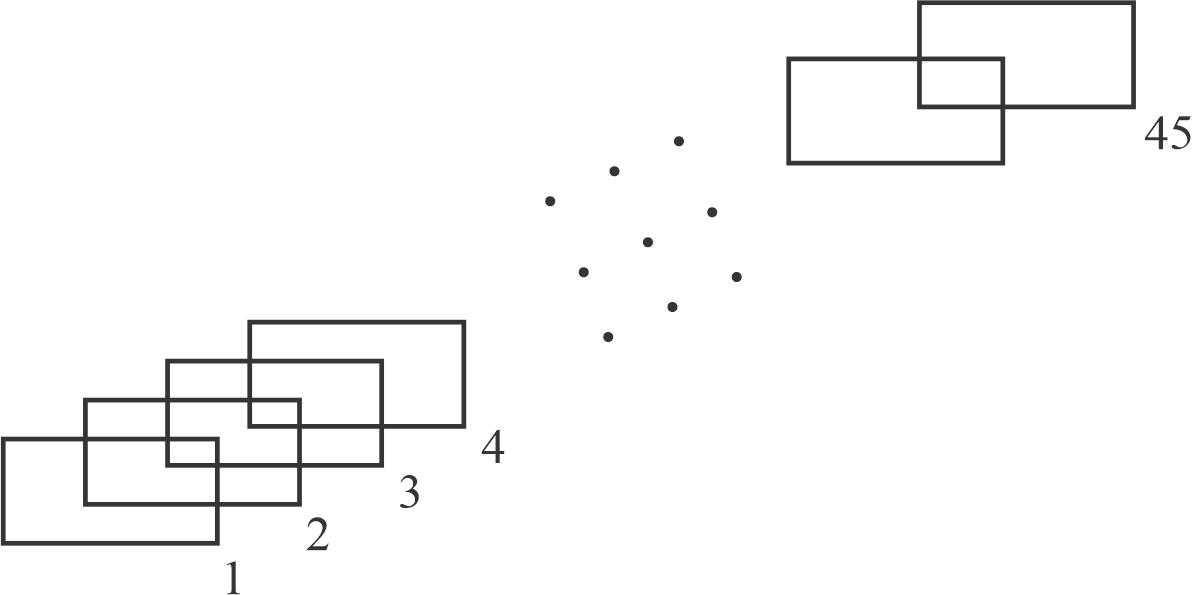
\includegraphics[width=5.5cm]{imagenes/general2024-I/etapa1/bio/razonamientomatematico4g24-I}
	\end{figure}
	
	\begin{enumerate}[label=\alph*)]
		\item 168
		\item 318
		\item 268
		\item 350
		\item 218
	\end{enumerate}
	
	\textbf{Respuesta correcta:} e)
	
	\vspace{2mm}
	\textbf{Solucionario:}\\
	
	Del gráfico se deduce:
	
	\begin{figure}[h]
		\centering
		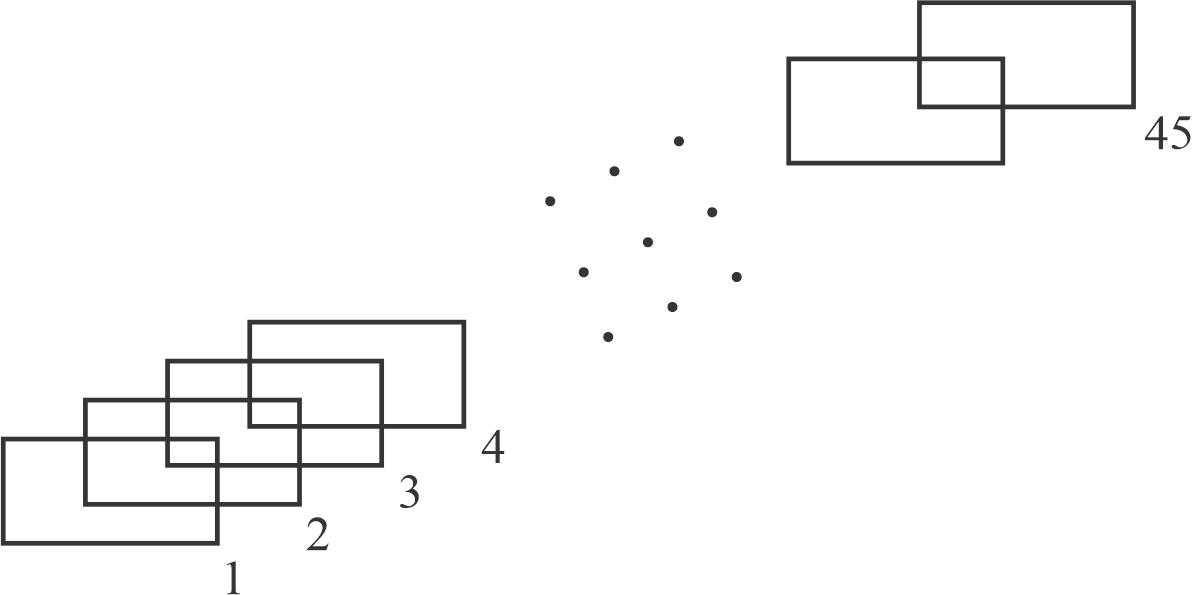
\includegraphics[width=5.5cm]{imagenes/general2024-I/etapa1/bio/razonamientomatematico4g24-I}
	\end{figure}
	
\end{enumerate}

\newpage

\begin{enumerate}[resume]
	
	\item La figura mostrada \textit{ABCD} es un cuadrado, donde \textit{P} y \textit{Q} son puntos medios. ¿Qué porcentaje del área del cuadrado es el área de las regiones sombreadas?
	
	\begin{figure}[h]
		\centering
		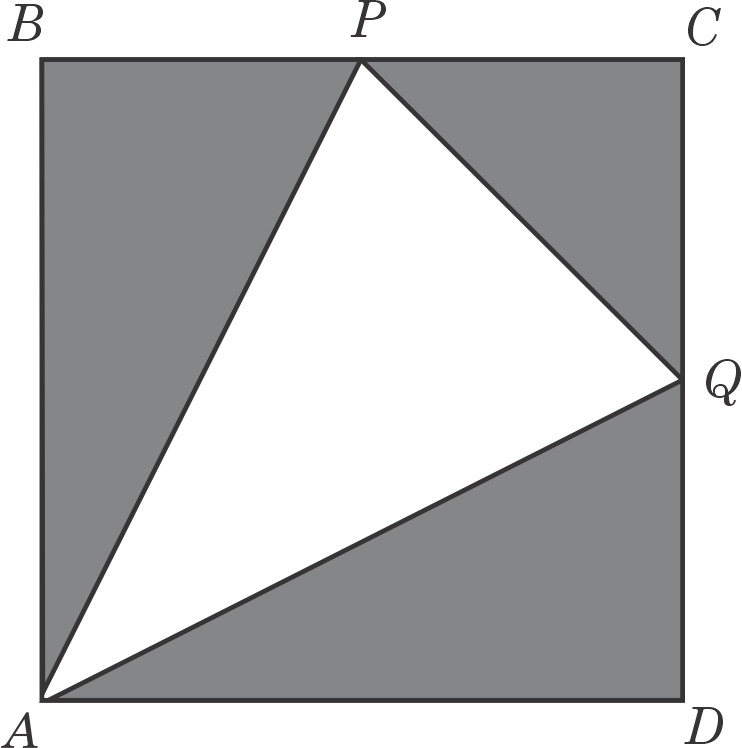
\includegraphics[width=3.5cm]{imagenes/general2024-I/etapa1/bio/razonamientomatematico5g24-I}
	\end{figure}
	
	\begin{enumerate}[label=\alph*)]
		\item $72\%$
		\item $52.5\%$
		\item $75\%$
		\item $62.5\%$
		\item $60\%$
	\end{enumerate}
	
	\textbf{Respuesta correcta:} d)
	
	\vspace{2mm}
	\textbf{Solucionario:}\\
	
	\noindent
	\begin{minipage}[t]{0.40\textwidth}
		\vspace{12pt}
		Según el gráfico:
		
		$50\%+\dfrac{1}{4}50\%$
		
		$50\%+12,5\%=62.5\%$
	\end{minipage}
	\hfill
	\begin{minipage}[t]{0.35\textwidth}
		\vspace{0pt}
		\centering
		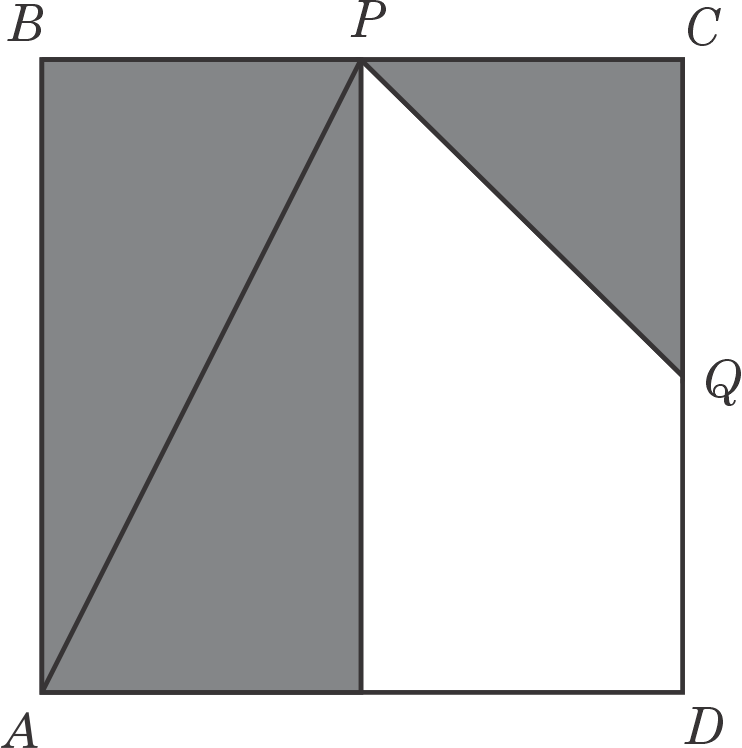
\includegraphics[width=3.5cm]{imagenes/general2024-I/etapa1/bio/razonamientomatematico5soluciong24-I}
	\end{minipage}
	
\end{enumerate}

\begin{enumerate}[resume]
	
	\item Calcule $x$:
	
	$\dfrac{x(x-1)!(x!-21)}{4!}=1+2!$
	
	\begin{enumerate}[label=\alph*)]
		\item 5
		\item 4
		\item 6
		\item 2
		\item 12
	\end{enumerate}
	
	\textbf{Respuesta correcta:} b)
	
	\vspace{2mm}
	\textbf{Solucionario:}\\
	
	$\dfrac{x(x-1)!(x!-21)}{4!}=1+2!$
	
	$\dfrac{x(x-1)!(x!-21)}{24}=1+2$
	
	$x!(x!-21)=72$
	
	$(x!)^2-21x!-72=0$
	
	Entonces:
	
	$(x!-24)(x!+3)=0$
	
	$x!=24 \qquad \text{o} \qquad x!=-3$
	
	Como $x!>0$, se tiene:
	
	$x!=24$
	
	$4!=24$
	
	$\therefore x=4$
	
\end{enumerate}


\subsection*{Razonamiento Verbal}

\begin{enumerate}[resume]
	
	\item Muchos de nuestros políticos son unos demagogos. Etimológicamente la palabra demagogo significa:
	
	\begin{enumerate}[label=\alph*)]
		\item \begin{tabular}{p{2.5cm} cp{3cm}} pueblo & -- & maestro. \end{tabular}
		\item \begin{tabular}{p{2.5cm} cp{3cm}} libertad & -- & ahora. \end{tabular}
		\item \begin{tabular}{p{2.5cm} cp{3cm}} democracia & -- & participativa. \end{tabular}
		\item \begin{tabular}{p{2.5cm} cp{3cm}} pueblo & -- & conductor. \end{tabular}
		\item \begin{tabular}{p{2.5cm} cp{3cm}} niño & -- & conductor. \end{tabular}
	\end{enumerate}
	
	\textbf{Respuesta correcta:} d)
	
	\vspace{2mm}
	\textbf{Solucionario:}\\[1mm]
	La pregunta pide el significado \textbf{etimológico} de la palabra \textit{demagogo}; es decir, su sentido a partir de las raíces griegas que la componen.
	
	La palabra \textit{demagogo} proviene del griego:
	
	\begin{itemize}[label=--]
		\item \textit{demos}: pueblo.
		\item \textit{agogos}: conductor, guía, el que conduce.
	\end{itemize}
	
	Por tanto, etimológicamente, \textit{demagogo} significa literalmente:
	
	\[
	\text{demagogo} = \text{pueblo} + \text{conductor}
	\]
	
	Es decir, \textbf{conductor del pueblo} o \textbf{el que guía al pueblo}.
	
	\vspace{6mm}
	
	\item Complete la oración\\
	A los psicólogos sociales podría considerárseles los médicos de la sociedad ... son los encargados de sanar los males que atacan a grupos humanos; ... ellos solo proporcionan los medios para que cada conglomerado humano saque sus propias conclusiones. 
	
	\begin{enumerate}[label=\alph*)]
		\item \begin{tabular}{p{2.5cm} cp{3cm}} ya que & -- & y \end{tabular}
		\item \begin{tabular}{p{2.5cm} cp{3cm}} pues & -- & por el contrario \end{tabular}
		\item \begin{tabular}{p{2.5cm} cp{3cm}} en tanto & -- & en consecuencia \end{tabular}
		\item \begin{tabular}{p{2.5cm} cp{3cm}} pero & -- & no obstante \end{tabular}
		\item \begin{tabular}{p{2.5cm} cp{3cm}} porque & -- & aunque \end{tabular}
	\end{enumerate}
	
	\textbf{Respuesta correcta:} e)
	
	\vspace{2mm}
	\textbf{Solucionario:}\\[1mm]
	Para resolver este tipo de ejercicios, debemos identificar la \textbf{relación lógica} entre las partes de la oración.
	
	\textit{A los psicólogos sociales podría considerárseles los médicos de la sociedad \textbf{porque} son los encargados de sanar los males que atacan a grupos humanos; \textbf{aunque} ellos solo proporcionan los medios para que cada conglomerado humano saque sus propias conclusiones.}
	
	La oración queda coherente:
	
	\begin{itemize}[label=--]
		\item \textbf{porque} explica la causa;
		\item \textbf{aunque} introduce una precisión restrictiva.
	\end{itemize}
	
	Revisemos por qué las demás no son las mejores:
	
	\begin{itemize}[label=--]
		\item a) \textit{ya que -- y}: el segundo conector solo suma, pero no expresa restricción.
		\item b) \textit{pues -- por el contrario}: el segundo establece oposición muy fuerte, no una concesión.
		\item c) \textit{en tanto -- en consecuencia}: el segundo indica resultado, lo cual no corresponde.
		\item d) \textit{pero -- no obstante}: ambos son adversativos; el primero no expresa adecuadamente la causa.
	\end{itemize}
	
	Por lo tanto, la alternativa correcta es \textbf{e)}.
	
	\vspace{6mm}
	
	\item Resuelve el siguiente par analógico.\\
	ADENITIS : GLÁNDULAS ::
	
	\begin{enumerate}[label=\alph*)]
		\item \begin{tabular}{p{2.5cm} cp{3cm}} cistitis & : & cejas. \end{tabular}
		\item \begin{tabular}{p{2.5cm} cp{3cm}} otitis & : & oídos. \end{tabular}
		\item \begin{tabular}{p{2.5cm} cp{3cm}} meningitis & : & meniscos. \end{tabular}
		\item \begin{tabular}{p{2.5cm} cp{3cm}} poliomelitis & : & huesos. \end{tabular}
		\item \begin{tabular}{p{2.5cm} cp{3cm}} blefaritis & : & labios. \end{tabular}
	\end{enumerate}
	
	\textbf{Respuesta correcta:} b)
	
	\vspace{2mm}
	\textbf{Solucionario:}\\[1mm]
	La relación analógica planteada es:
	
	\[
	\text{nombre de enfermedad o inflamación} : \text{órgano o parte afectada}
	\]
	
	Analicemos el primer par:
	
	\begin{itemize}[label=--]
		\item \textit{Adenitis} = inflamación de las glándulas.
	\end{itemize}
	
	Entonces debemos buscar otra relación semejante:
	
	\[
	\text{inflamación} : \text{órgano afectado}
	\]
	
	Revisemos las opciones:
	
	\begin{itemize}[label=--]
		\item a) \textit{cistitis} : cejas\\
		Cistitis es inflamación de la vejiga, no de las cejas.
		
		\item b) \textit{otitis} : oídos\\
		Otitis es inflamación del oído. La relación es correcta.
		
		\item c) \textit{meningitis} : meniscos\\
		Meningitis es inflamación de las meninges, no de los meniscos.
		
		\item d) \textit{poliomielitis} : huesos\\
		La poliomielitis afecta el sistema nervioso, no los huesos.
		
		\item e) \textit{blefaritis} : labios\\
		Blefaritis es inflamación de los párpados, no de los labios.
	\end{itemize}
	
	La única alternativa que conserva exactamente la misma relación es:
	
	\[
	\text{otitis} : \text{oídos}
	\]
	
	Por ello, la respuesta correcta es \textbf{b)}.
	
	\vspace{6mm}
	
	\item ELIMINACIÓN DE ORACIONES
	
	\begin{enumerate}[label=\alph*)]
		\item El problema surge a partir de la observación.
		\item El conocimiento surge a partir de la investigación.
		\item Una buena investigación implica observación.
		\item Los sentidos deben estar en óptimo nivel para percibir.
		\item La observación debe ser objetiva.
	\end{enumerate}
	
	\textbf{Respuesta correcta:} d)
	
	\vspace{2mm}
	\textbf{Solucionario:}\\[1mm]
	En eliminación de oraciones debemos identificar cuál de los enunciados \textbf{rompe la unidad temática} o se aleja de la idea central.
	
	Observemos el tema común de las oraciones:
	
	\begin{itemize}[label=--]
		\item a) relaciona la observación con el surgimiento del problema.
		\item b) relaciona la investigación con el conocimiento.
		\item c) vincula directamente investigación y observación.
		\item e) señala una característica propia de la observación: la objetividad.
	\end{itemize}
	
	En todas ellas el eje temático es el \textbf{proceso de observación e investigación} como base del conocimiento.
	
	En cambio, la oración:
	
	\textit{Los sentidos deben estar en óptimo nivel para percibir}
	
	se enfoca en una condición biológica o fisiológica de la percepción sensorial, no en la observación como método de investigación ni en su valor epistemológico.
	
	Es decir:
	
	\begin{itemize}[label=--]
		\item no desarrolla directamente la idea de investigación;
		\item no explica la objetividad de la observación;
		\item no se integra con precisión al conjunto.
	\end{itemize}
	
	Por eso, la oración que se debe eliminar es la \textbf{d)}.
	
	\vspace{6mm}
	
	\item El sinónimo de la palabra MEFÍTICO es:
	
	\begin{enumerate}[label=\alph*)]
		\item inodoro.
		\item corrosivo.
		\item insípido.
		\item irrespirable.
		\item expansivo.
	\end{enumerate}
	
	\textbf{Respuesta correcta:} d)
	
	\vspace{2mm}
	\textbf{Solucionario:}\\[1mm]
	La palabra \textit{mefítico} se usa para describir algo que:
	
	\begin{itemize}[label=--]
		\item despide emanaciones fétidas o nocivas;
		\item tiene un olor desagradable;
		\item resulta dañino o difícil de respirar.
	\end{itemize}
	
	Por ello, el significado más próximo es:
	
	\[
	\text{mefítico} \approx \text{irrespirable}
	\]
	
	Revisemos las opciones:
	
	\begin{itemize}[label=--]
		\item a) \textit{inodoro}: significa sin olor, contrario a mefítico.
		\item b) \textit{corrosivo}: alude a lo que desgasta o quema, no al olor o al aire.
		\item c) \textit{insípido}: significa sin sabor.
		\item d) \textit{irrespirable}: que no se puede respirar o resulta nocivo al respirar. Es la mejor equivalencia.
		\item e) \textit{expansivo}: no guarda relación semántica.
	\end{itemize}
	
	Por lo tanto, el sinónimo correcto es \textbf{d) irrespirable}.
	
	\vspace{6mm}
	
	\item \hfill TEXTO \hfill \null
	
	La biología moderna se basa en la suposición de que las funciones de los sistemas vivos pueden ser explicadas en términos de procesos físicos y químicos. El organismo vivo por lo tanto se considera como un sistema químico altamente complejo y bien organizado. Pero, al reducir el estudio de las reacciones químicas individuales, inevitablemente surge una pregunta: ¿Dónde termina lo que hace vivo a un organismo y dónde comienza lo que no lo hace?; o, haciendo la pregunta de otra manera: ¿Cuándo un conjunto de moléculas deja de ser solamente una mezcla química y se convierte en un organismo vivo?\\
	La pregunta inevitable obligatoria a la biología a:
	
	\begin{enumerate}[label=\alph*)]
		\item comparar a los seres vivos.
		\item definir lo que es la vida.
		\item caracterizar a los seres vivos.
		\item identificar el principio de la vida.
		\item comprender los procesos químicos.
	\end{enumerate}
	
	\textbf{Respuesta correcta:} b)
	
	\vspace{2mm}
	\textbf{Solucionario:}\\[1mm]
	El texto presenta una reflexión central de la biología moderna. Primero afirma que los sistemas vivos pueden explicarse mediante procesos físicos y químicos; sin embargo, después plantea una dificultad fundamental:
	
	\begin{itemize}[label=--]
		\item ¿dónde termina lo no vivo y empieza lo vivo?;
		\item ¿cuándo un conjunto de moléculas pasa de ser simple materia a convertirse en un organismo vivo?
	\end{itemize}
	
	Estas preguntas muestran que el problema central no es únicamente describir reacciones químicas, sino establecer con claridad qué debe entenderse por \textbf{vida}.
	
	Analicemos las alternativas:
	
	\begin{itemize}[label=--]
		\item a) \textit{comparar a los seres vivos}: no es la idea principal del texto.
		\item b) \textit{definir lo que es la vida}: sí, porque el texto cuestiona precisamente el límite entre lo vivo y lo no vivo.
		\item c) \textit{caracterizar a los seres vivos}: es una consecuencia posible, pero no el punto central.
		\item d) \textit{identificar el principio de la vida}: suena cercano, pero el texto no pide hallar un principio aislado, sino definir conceptualmente la vida.
		\item e) \textit{comprender los procesos químicos}: eso ya se menciona al inicio, pero la pregunta va más allá.
	\end{itemize}
	
	En conclusión, la interrogante planteada obliga a la biología a \textbf{definir lo que es la vida}.\\
	Por tanto, la respuesta correcta es \textbf{b)}.
	
\end{enumerate}


\subsection*{Inglés}

\begin{enumerate}[resume]
	
	\item What is the alternative is talking in simple past tense?
	
	\begin{enumerate}[label=\alph*)]
		\item We worked in this hospital.
		\item We work in this hospital.
		\item We will work en this hospital.
		\item We won't work in this hospital.
		\item We are working in this hospital.
	\end{enumerate}
	
	\textbf{Respuesta correcta:} a)
	
	\vspace{2mm}
	\textbf{Solucionario:}
	
	The simple past tense is used to express actions completed in the past. The sentence \textit{We worked in this hospital} uses the verb \textit{worked}, which is the past form of \textit{work}. Therefore, the correct answer is option a).
	
\end{enumerate}

\begin{enumerate}[resume]
	
	\item Which are the derivated products of the milk?
	
	\begin{enumerate}[label=\alph*)]
		\item Cheese - yogurt - milk - butter
		\item Orange - pasta - bread - apple
		\item Tomato - corn - onion - carrot
		\item Rice - sugars - potatoes - egg
		\item Chicken - cheese - fish - salmon
	\end{enumerate}
	
	\textbf{Respuesta correcta:} a)
	
	\vspace{2mm}
	\textbf{Solucionario:}
	
	Milk products or dairy products include cheese, yogurt and butter. Among the alternatives, only option a) contains foods derived from milk. Therefore, the correct answer is a).
	
\end{enumerate}


\subsection*{Quechua y Aimara}

\begin{enumerate}[resume]
	
	\item ¿Hay'ka ñawikunayuq huk runari kan? / ¿Qawqha nayranakanisa mä jaqixa?
	
	\begin{enumerate}[label=\alph*)]
		\item Iskay ñawikunayuq / paya nayranaka.
		\item Kimsa ñawikunayuq / kimsa nayranaka.
		\item Tawa ñawikunayuq / pusi nayranaka.
		\item Pichqa ñawikunayuq / phisqa nayranaka.
		\item Suqta ñawikunayuq / suxta nayranaka.
	\end{enumerate}
	
	\textbf{Respuesta correcta:} b)
	
	\vspace{2mm}
	\textbf{Solucionario:}
	
	La pregunta pide cuántos ojos tiene una persona. Según la clave marcada, la respuesta correcta es \textit{kimsa ñawikunayuq / kimsa nayranaka}. Por lo tanto, en el desarrollo se conserva la alternativa correcta señalada en el material.
	
\end{enumerate}

\begin{enumerate}[resume]
	
	\item ¿Hay'ka tullukunataq runaq kurkunpiri kan? / ¿Qawqha ch'akasa janchisana utji?
	
	\begin{enumerate}[label=\alph*)]
		\item Iskay pachak iskayniyuq tullukuna / pä pataka payani ch'akanaka.
		\item Iskay pachak kimsayuq tullukuna / pä pataka kimsani ch'akanaka.
		\item Iskay pachak tawayuq tullukuna / pä pataka pusini ch'akanaka.
		\item Iskay pachak tullukuna / pä pataka ch'akanaka.
		\item Iskay pachak suqtayuq tullukuna / pä pataka suxtani ch'akanaka.
	\end{enumerate}
	
	\textbf{Respuesta correcta:} e)
	
	\vspace{2mm}
	\textbf{Solucionario:}
	
	La pregunta se refiere a la cantidad de huesos del cuerpo humano. Según la clave señalada en el material, corresponde la alternativa e): \textit{Iskay pachak suqtayuq tullukuna / pä pataka suxtani ch'akanaka}. En consecuencia, se mantiene esa respuesta como la correcta.
	
\end{enumerate}
	




\section*{Área: Sociales}

\subsection*{Aritmética}

\begin{enumerate}
	
	\item Si los conjuntos $A$ y $B$ tienen 24 y 32 elementos respectivamente, ¿Cuántos elementos tendrá $A\cup B$, sabiendo que $A\cap B$ tiene 14 elementos?
	\begin{enumerate}[label=\alph*)]
		\item 42
		\item 38
		\item 36
		\item 40
		\item 44
	\end{enumerate}
	\textbf{Respuesta correcta:} a)
	
	\vspace{2mm}
	\textbf{Solucionario:}\\[1mm]
	
	$n(A)=24,\ \ n(B)=32,\ \ n(A\cap B)=14$
	
	Sabemos que $n(A\cup B)=n(A)+n(B)-n(A\cap B)$
	
	$\Rightarrow\ n(A\cup B)=24+32-14$
	
	\fbox{$n(A\cup B)=42$} elementos
	
	\vspace{6mm}
	
	\item A un alambre de $95m$ de longitud, se le han dado 2 cortes de manera que la longitud de cada trozo sea igual al anterior aumentado en su mitad. ¿Cuál es la longitud del trozo más largo?
	\begin{enumerate}[label=\alph*)]
		\item $25m$
		\item $30m$
		\item $45m$
		\item $55m$
		\item $40m$
	\end{enumerate}
	\textbf{Respuesta correcta:} c)
	
	\vspace{2mm}
	\textbf{Solucionario:}\\[1mm]
	
\begin{tikzpicture}[x=0.09cm,y=1cm]
	
	% línea total
	\draw[thick] (0,2.2) -- (95,2.2);
	\draw[thick] (0,2.1) -- (0,2.3);
	\draw[thick] (95,2.1) -- (95,2.3);
	\node at (47.5,2.55) {$95m$};
	
	% línea base
	\draw[thick] (0,1.4) -- (95,1.4);
	
	% marcas pequeñas uniformes
	\draw[thick] (0,1.3) -- (0,1.5);
	\draw[thick] (20,1.3) -- (20,1.5);
	\draw[thick] (50,1.3) -- (50,1.5);
	\draw[thick] (95,1.3) -- (95,1.5);
	
	% etiquetas
	\node at (10,1) {$x$};
	\node at (35,1) {$x+\dfrac{x}{2}$};
	\node at (72.5,1) {$\left(x+\dfrac{x}{2}\right)+\dfrac{1}{2}\left(x+\dfrac{x}{2}\right)$};
	
\end{tikzpicture}
	
	Luego:
	
	$x+\left(x+\dfrac{x}{2}\right)+\left(\left(x+\dfrac{x}{2}\right)+\dfrac{1}{2}\left(x+\dfrac{x}{2}\right)\right)=95$
	
	$\dfrac{4x+4x+2x+4x+2x+2x+x}{4}=95$
	
	$19x=380 \Rightarrow x=20$
	
	Trozo más largo:
	
	$x+\dfrac{x}{2}+\dfrac{1}{2}\left(x+\dfrac{x}{2}\right)$\fbox{$=45m$}
	
	\vspace{6mm}
	
	\item De 25 televisores que se fabrican, uno sale defectuoso. ¿Cuál es la probabilidad de escoger un televisor defectuoso de un total de 100 televisores fabricados?
	\begin{enumerate}[label=\alph*)]
		\item $1\%$
		\item $2\%$
		\item $4\%$
		\item $8\%$
		\item $5\%$
	\end{enumerate}
	\textbf{Respuesta correcta:} c)
	
	\vspace{2mm}
	\textbf{Solucionario:}\\[1mm]
	
	Se tiene
	
	\begin{tikzpicture}[x=0.08cm,y=1cm]
		
		% línea principal
		\draw[thick] (0,1.6) -- (100,1.6);
		
		% marca central
		\draw[thick] (25,1.6) -- (25,2.0);
		
		% cuadro total
		\draw[thick] (19,2.0) rectangle (31,2.6);
		\node at (25,2.3) {$25\times 4$};
		\node at (25,2.85) {Total};
		
		% cuadro defecto
		\draw[thick] (0,1.0) rectangle (12,1.6);
		\node at (6,1.3) {$1\times 4$};
		\node at (6,1.85) {defecto};
		
		% cuadro sin defecto
		\draw[thick] (86,1.0) rectangle (100,1.6);
		\node at (93,1.3) {$24\times 4$};
		\node at (93,1.85) {Sin defecto};
		
	\end{tikzpicture}
	
	
	Luego
	
	$(n^\circ \text{ de casos Totales})=(n^\circ \text{ total de Televisores})=100$
	
	Además
	
	$(n^\circ \text{ de casos favorables})=(n^\circ \text{ de Televisores con defecto})=4$
	
	$\Rightarrow (\text{probabilidad pedida})=\dfrac{4}{100}=\dfrac{1}{25}$\fbox{$=4\%$}
	
	\vspace{6mm}
	
\end{enumerate}





\subsection*{Álgebra}

\begin{enumerate}[resume]
	
	\item ¿Cuántos términos del desarrollo de $(3\sqrt{3}+\sqrt{2})^{12}$ son números naturales?
	\begin{enumerate}[label=\alph*)]
		\item 7
		\item 6
		\item 3
		\item 4
		\item 5
	\end{enumerate}
	\textbf{Respuesta correcta:} a)
	
	\vspace{2mm}
	\textbf{Solucionario:}\\[1mm]
	
	$T_{k+1}=C_k^{12}a^{12-k}\cdot b^k$
	
	$\therefore\ T_{k+1}=C_k^{12}(3\sqrt{3})^{12-k}\cdot (\sqrt{2})^k$
	
	$=C_k^{12}\,3^{12-k}\cdot 3^{\dfrac{12-k}{2}}\cdot 2^{\dfrac{k}{2}}$
	
	Los valores $\dfrac{12-k}{2}$ y $\dfrac{k}{2}$ deben ser pares.
	
	\fbox{$\therefore\ k=\{0,2,4,6,8,10,12\}$}
	
	de donde 7 términos del desarrollo son números naturales.
	
	\vspace{6mm}
	
	\item Sean los polinomios $P(x)=2x^2-15$ y $Q(x,y)=2x+3y-2$. Halle el término independiente del polinomio $H(t)=Q(P(3),3t-1)$
	\begin{enumerate}[label=\alph*)]
		\item $-5$
		\item $-15$
		\item $-2$
		\item $1$
		\item $7$
	\end{enumerate}
	\textbf{Respuesta correcta:} d)
	
	\vspace{2mm}
	\textbf{Solucionario:}\\[1mm]
	
	$P(3)=2(3)^2-15=3$
	
	$H(t)=Q(3,3t-1)=2(3)+3(3t-1)-2$
	
	$=6+9t-3-2$
	
	$=9t+1$
	
	\fbox{$H(0)=1$} 
	
	\vspace{6mm}
	
	\item Dada la función $f(x)=4|x|-x^2,\ \ x\in\langle -4,4\rangle$ halle el valor de verdad de las siguientes proposiciones.
	
	I. $f(x)$ es una función impar.\\
	II. Para $x\geq 0$ en el dominio de la función, la gráfica de $f$ es una parábola que se abre hacia abajo.\\
	III. La gráfica de $f$ es simétrica respecto al eje $Y$.
	
	\begin{enumerate}[label=\alph*)]
		\item FVV
		\item FFF
		\item VFF
		\item VFV
		\item FVF
	\end{enumerate}
	\textbf{Respuesta correcta:} a)
	
	\vspace{2mm}
	\textbf{Solucionario:}\\[1mm]
	
	I. $f(-x)=4|-x|-(-x)^2=4x-x^2=f(x)$ \hfill (F)
	
	II. Si $x\geq 0 \Rightarrow f(x)=4x-x^2$ es una parábola que se abre hacia abajo \hfill (V)
	
	III. $f$ es par, por tanto hay simetría respecto al eje $Y$ \hfill (V)
	
	\vspace{6mm}
	
\end{enumerate}






\subsection*{Geometría}

\begin{enumerate}[resume]
	
	\item En la figura: \hspace{2mm} $AB=BD$, \hspace{2mm} $m\angle ACD=40^\circ$, \hspace{2mm} $m\angle BAC=m\angle CAD$ \hspace{2mm} y \hspace{2mm} $m\angle BDC=m\angle CDE$.\\
	Calcule $x$.
	
	\begin{center}
		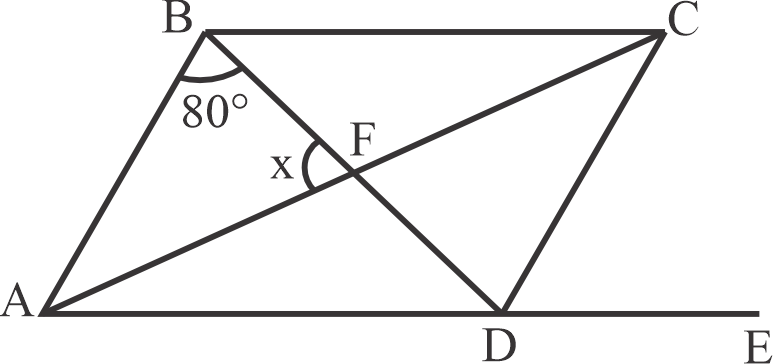
\includegraphics[width=4.5cm]{imagenes/general2024-I/etapa1/soc/geo1g24-I.png}
	\end{center}
	
	\begin{enumerate}[label=\alph*)]
		\item $75^\circ$
		\item $65^\circ$
		\item $30^\circ$
		\item $45^\circ$
		\item $60^\circ$
	\end{enumerate}
	\textbf{Respuesta correcta:} a)
	
	\vspace{2mm}
	\textbf{Solucionario:}\\[1mm]
	
	
	
		\begin{center}
		\begin{minipage}{0.45\textwidth}
		de la fig.
	
		$\bullet\ \ 4\alpha=180-80 \ \ \Rightarrow\ \ \alpha=25$
		
		$\bullet\ \ 3\alpha=x$
		
		$3(25)=x$
		
		\fbox{$75^\circ=x$}
			\vspace{6mm}
		\end{minipage}
		\hfill
		\begin{minipage}{0.45\textwidth}
			\centering
			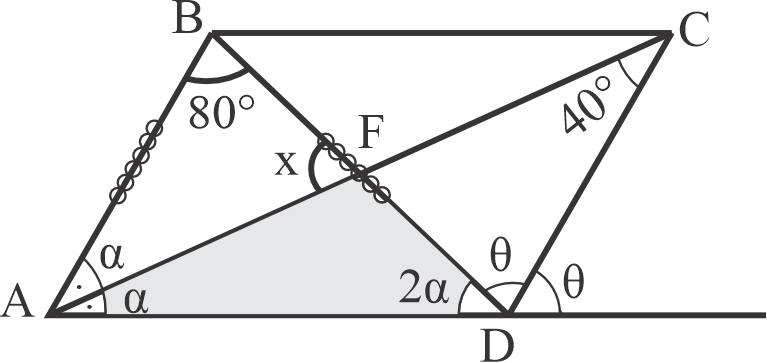
\includegraphics[width=4.5cm]{imagenes/general2024-I/etapa1/soc/geo1g24-Ir.png}
		\end{minipage}
	\end{center}
	
	
	\vspace{6mm}
	
	\item Halle el valor de verdad de las siguientes proposiciones:
	
	I. Un ángulo obtuso es aquel cuya medida es comprendida entre $0^\circ$ y $90^\circ$\\
	II. Los ángulos suplementarios son aquellos cuyas medidas suman $90^\circ$\\
	III. La intersección de las medianas de un triángulo se llama Incentro.\\
	IV. La cuerda mayor de una circunferencia se llama diámetro.
	
	\begin{enumerate}[label=\alph*)]
		\item VFVF
		\item FVFV
		\item FFVV
		\item VVFF
		\item FFFV
	\end{enumerate}
	\textbf{Respuesta correcta:} e)
	
	\vspace{2mm}
	\textbf{Solucionario:}\\[1mm]
	
	I) $\alpha$ es obtuso, por lo tanto \hfill (F)
	
	II) Ángulos suplementarios es: $180^\circ$ \hfill (F)
	
	III) no es incentro, se llama baricentro \hfill (F)
	
	IV) $D=$ cuerda mayor. \hfill (V)
	
	\vspace{6mm}
	
\end{enumerate}




\subsection*{Trigonometría}

\begin{enumerate}[resume]
	
	\item En la figura, calcule la longitud del segmento $BC$, si $\sen\alpha=0,5$ y $AD=5$
	
	\begin{center}
		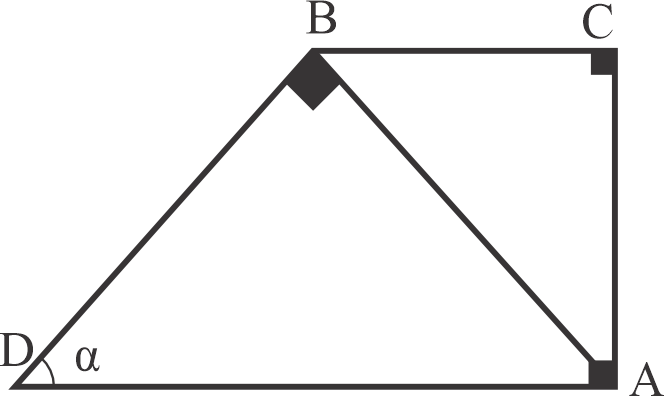
\includegraphics[width=4.3cm]{imagenes/general2024-I/etapa1/soc/trigo1g24-I.png}
	\end{center}
	
	\begin{enumerate}[label=\alph*)]
		\item $\dfrac{8}{5}$
		\item $\dfrac{10}{3}$
		\item $\dfrac{5}{4}$
		\item $\dfrac{3}{4}$
		\item $\dfrac{7}{6}$
	\end{enumerate}
	\textbf{Respuesta correcta:} c)
	
	\vspace{2mm}
	\textbf{Solucionario:}\\[1mm]

	
	\begin{center}
		\begin{minipage}{0.45\textwidth}
		$x=(5\sen\alpha)(\sen\alpha)$
	
		$=5\sen^2\alpha$
		
		$=5\left(\dfrac{1}{2}\right)^2$
	
		\fbox{$=\dfrac{5}{4}$}
			
			
			\vspace{6mm}
		\end{minipage}
		\hfill
		\begin{minipage}{0.45\textwidth}
			\centering
			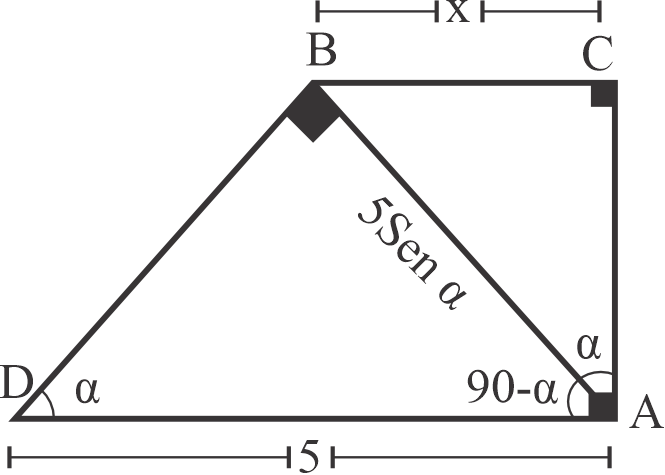
\includegraphics[width=4.3cm]{imagenes/general2024-I/etapa1/soc/trigo1g24-Ir.png}
		\end{minipage}
	\end{center}
	
	
	
	
	\vspace{6mm}
	
	\item Si $\alpha$ es un ángulo en el primer cuadrante y $\sin\alpha=0,25$ halle $\csc\alpha+\cot^2\alpha$
	
	\begin{enumerate}[label=\alph*)]
		\item $16$
		\item $\dfrac{9}{5}$
		\item $\dfrac{7}{8}$
		\item $19$
		\item $\dfrac{3}{8}$
	\end{enumerate}
	\textbf{Respuesta correcta:} d)
	
	\vspace{2mm}
	\textbf{Solucionario:}\\[1mm]
	

	
		\begin{center}
		\begin{minipage}{0.45\textwidth}
			$\csc\alpha+\cot^2\alpha$
			
			$=\dfrac{4}{1}+\left(\dfrac{\sqrt{15}}{1}\right)^2$
			
			$=4+15$
			
			\fbox{$=19$}
			
			
			\vspace{6mm}
		\end{minipage}
		\hfill
		\begin{minipage}{0.45\textwidth}
			\centering
			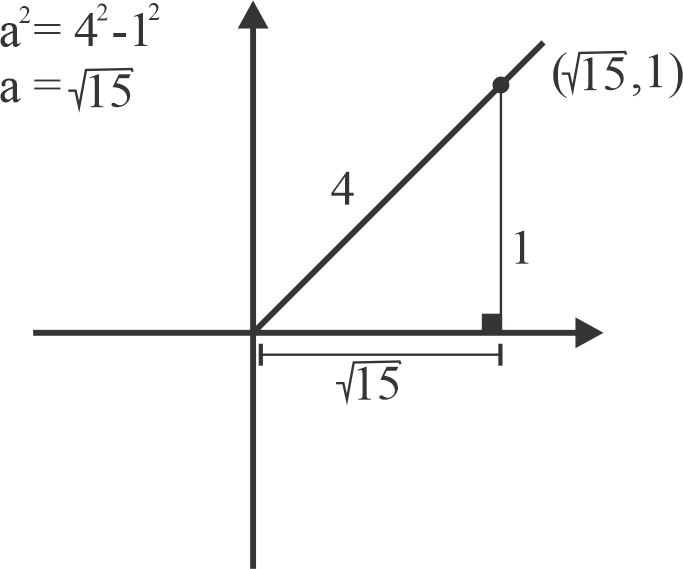
\includegraphics[width=4.5cm]{imagenes/general2024-I/etapa1/soc/trigo2g24-Ir.png}
		\end{minipage}
		\end{center}
	
	\vspace{6mm}
	
\end{enumerate}




\subsection*{Física}

\begin{enumerate}[resume]
	
\item Se tiene una puerta de plancha de acero de $300\ cm$ de largo y $200\ cm$ de alto a una temperatura de $0^\circ C$. Calcule el aumento de su área cuando el sol calienta hasta una temperatura de $100^\circ C$.

$(\alpha_{acero}=1{,}2\times10^{-5}\ ^\circ C^{-1})$

\begin{enumerate}[label=\alph*)]
	\item $141\ cm^2$
	\item $144\ cm^2$
	\item $143\ cm^2$
	\item $140\ cm^2$
	\item $142\ cm^2$
\end{enumerate}
\textbf{Respuesta correcta:} b)

\vspace{2mm}
\textbf{Solucionario:}\\[1mm]

\begin{tikzpicture}[x=0.01cm,y=0.01cm]
	
	% Marco exterior de la puerta
	\draw[very thick] (0,0) rectangle (300,200);
	
	% Borde interno
	\draw[thick] (8,8) rectangle (292,192);
	
	% División central
	\draw[thick] (150,8) -- (150,192);
	
	% Detalles diagonales tipo panel
	\draw[thick] (8,8) -- (150,100);
	\draw[thick] (150,100) -- (292,192);
	
	\draw[thick] (8,192) -- (150,100);
	\draw[thick] (150,100) -- (292,8);
	
	% Perilla
	\filldraw[black] (170,100) circle (6);
	
	% Medidas
	\draw[thick] (0,-20) -- (300,-20);
	\draw[thick] (0,-15) -- (0,-25);
	\draw[thick] (300,-15) -- (300,-25);
	\node at (150,-35) {$300\ cm$};
	
	\draw[thick] (320,0) -- (320,200);
	\draw[thick] (315,0) -- (325,0);
	\draw[thick] (315,200) -- (325,200);
	\node[rotate=90] at (338,100) {$200\ cm$};
	
	\end{tikzpicture}

Área inicial:

$A_0=(300)(200)=60000\ cm^2$

$A_0=6\times10^4\ cm^2$

Cambio de temperatura:

$\Delta T=100^\circ C-0^\circ C=100^\circ C$

Para dilatación superficial:

$\beta=2\alpha$

$\beta=2(1{,}2\times10^{-5})$

$\beta=2{,}4\times10^{-5}\ ^\circ C^{-1}$

Usamos:

$\beta=\dfrac{\Delta A}{A_0\Delta T}$


$\Delta A=\beta A_0\Delta T$


$\Delta A=(2{,}4\times10^{-5})(6\times10^4)(100)$

$\Delta A=(2{,}4)(6)(10^{-5+4})(100)$

$\Delta A=14{,}4(10^{-1})(100)$

$\Delta A=1{,}44(100)$

\fbox{$\Delta A=144\ cm^2$}

\vspace{6mm}
	
	
	
	
	\item Una pelota de $0{,}5\ kg$ atada a una cuerda de $0{,}5\ m$ de radio gira uniformemente en un plano vertical con una rapidez tangencial de $10\ m/s$. Determine el módulo de la tensión de la cuerda en la posición más alta de su trayectoria. $(g=10\ m/s^2)$
	
	\begin{enumerate}[label=\alph*)]
		\item $90\ N$
		\item $92\ N$
		\item $95\ N$
		\item $94\ N$
		\item $93\ N$
	\end{enumerate}
	\textbf{Respuesta correcta:} c)
	
	\vspace{2mm}
	\textbf{Solucionario:}\\[1mm]
	
	\begin{tikzpicture}[scale=0.7]
		\draw[thick] (0,0) circle (2);
		\filldraw[black] (0,2) circle (5pt);
		\draw[->, thick] (0,2) -- (0,0.8);
		\draw[->, thick] (0,2) -- (0,1.2);
		\draw[->, thick] (0,2) -- (1,2);
		\draw[-, thick] (0,2) -- (0,-0.1);
		\node at (0.25,1.45) {$T$};
		\node at (-0.60,1.45) {$F_N$};
		\node at (-0.25,1.05) {$W$};
		\node at (1.2,2.15) {$v$};
	\end{tikzpicture}
	
	
	$\sum F_c=T+W=\dfrac{mv^2}{R}$
	
	$\sum F_c=T+mg=\dfrac{mv^2}{R}$
	
	
	$T=\dfrac{mv^2}{R}-mg$
	
	$T=m\left(\dfrac{v^2}{R}-g\right)$
	
	$m=0{,}5\ kg,\qquad v=10\ m/s,\qquad R=0{,}5\ m,\qquad g=10\ m/s^2$
	
	$T=0{,}5\left(\dfrac{10^2}{0{,}5}-10\right)$
	
	$T=0{,}5\left(\dfrac{100}{0{,}5}-10\right)$
	
	$T=0{,}5(200-10)$
	
	$T=0{,}5(190)$
	
	\fbox{$T=95\ N$}
	
	\vspace{6mm}
	
	
	
	
	
	
\end{enumerate}


\subsection*{Química}

\begin{enumerate}[resume]
	
	\item Indique las propiedades químicas del carbono.
	
	I. tetravalencia\\
	II. covalencia\\
	III. peso específico\\
	IV. autosaturación
	
	\begin{enumerate}[label=\alph*)]
		\item I, II y III
		\item II, III y IV
		\item III y IV
		\item I, II y IV
		\item II y IV
	\end{enumerate}
	\textbf{Respuesta correcta:} d)
	
	\vspace{2mm}
	\textbf{Solucionario:}\\[1mm]
	
	Las propiedades químicas del átomo de carbono son:
	
	I) tetravalencia.\\
	II) covalencia.\\
	IV) autosaturación.
	
	No se considera el peso específico como propiedad química.
	
	\vspace{6mm}
	
	\item Determine el volumen de 1 mol de una sustancia a la presión de $1,5$ atmósferas y $27^\circ C$
	
	\begin{enumerate}[label=\alph*)]
		\item $13,6L$
		\item $17,4L$
		\item $14,6L$
		\item $15,4L$
		\item $16,4L$
	\end{enumerate}
	\textbf{Respuesta correcta:} e)
	
	\vspace{2mm}
	\textbf{Solucionario:}\\[1mm]
	
	Datos
	
	$P=1,5\ atm$
	
	$R\text{ constante}=0.082\ \dfrac{L\cdot atm}{mol\cdot K}$
	
	$T=27^\circ C=300^\circ K$
	
	$\Rightarrow$ si \hspace{2mm} $PV=nRT$
	
	despejando el $V=\dfrac{nRT}{P}$
	
	$V=\dfrac{1\ mol\cdot 0.082\ \dfrac{L\cdot atm}{mol\cdot K}\cdot 300^\circ K}{1.5\ atm}$
	
	\fbox{$V=16.4\ L$}
	
	\vspace{6mm}
	
\end{enumerate}





\subsection*{Biología y Anatomía}

\begin{enumerate}[resume]
	
	\item La relación estrecha entre dos especies en la cual la evolución de una promueve la evolución de la otra, hasta llegar a un estado de interdependencia, se denomina:
	\begin{enumerate}[label=\alph*)]
		\item Evolución adaptativa
		\item Evolución paralela
		\item Evolución advergente
		\item Coevolución
		\item Convergencia evolutiva
	\end{enumerate}
	\textbf{Respuesta correcta:} d)
	
	\vspace{2mm}
	\textbf{Solucionario:}\\[1mm]
	La \textbf{coevolución} ocurre cuando dos especies interactúan de manera tan estrecha que los cambios evolutivos en una influyen en la otra, generando interdependencia.
	
	\vspace{6mm}
	
	\item ¿Cuál es el conducto que se dirige hacia el duodeno y desemboca junto con el conducto pancreático, en el área denominada ampolla Vater?
	\begin{enumerate}[label=\alph*)]
		\item De Herring
		\item Hepático común
		\item Cístico
		\item Colédoco
		\item De Wharton
	\end{enumerate}
	\textbf{Respuesta correcta:} d)
	
	\vspace{2mm}
	\textbf{Solucionario:}\\[1mm]
	El \textbf{conducto colédoco} transporta la bilis hacia el duodeno y se une con el conducto pancreático en la ampolla de Vater.
	
	\vspace{6mm}
	
\end{enumerate}

\subsection*{Psicología y Filosofía}

\begin{enumerate}[resume]
	
	
	\item Un niño aprende que, si llora, su mamá le prestará atención y lo mimará inclusive le dará un caramelo “Para que se sienta mejor”. En este caso, el niño controla perfectamente la situación y su entorno.\\
	Este comportamiento corresponde al condicionamiento:
	\begin{enumerate}[label=\alph*)]
		\item Placentero.
		\item Operante
		\item Experimental
		\item Clásico
		\item Reforzado
	\end{enumerate}
	\textbf{Respuesta correcta:} b)
	
	\vspace{2mm}
	\textbf{Solucionario:}\\[1mm]
	Es \textbf{condicionamiento operante} porque el niño realiza una conducta y obtiene una consecuencia favorable, reforzando ese comportamiento.
	
	\vspace{6mm}
	
	\item En la actualidad, un porcentaje elevado de personas realizan simultáneamente dos cosas. Por ejemplo, escribir y contestar el teléfono. En este caso, se hace uso de la atención.
	\begin{enumerate}[label=\alph*)]
		\item Refleja
		\item Dividida
		\item Selectiva
		\item Sostenida
		\item Automática
	\end{enumerate}
	\textbf{Respuesta correcta:} b)
	
	\vspace{2mm}
	\textbf{Solucionario:}\\[1mm]
	La \textbf{atención dividida} permite atender dos tareas al mismo tiempo.
	
	\vspace{6mm}
	
	\item Adriana es mucho más bella que María. ¿Qué característica del valor se resalta en el enunciado anterior?
	\begin{enumerate}[label=\alph*)]
		\item Subjetivo
		\item Objetivo
		\item Gradual
		\item Jerárquico
		\item Polaridad
	\end{enumerate}
	\textbf{Respuesta correcta:} c)
	
	\vspace{2mm}
	\textbf{Solucionario:}\\[1mm]
	La expresión “mucho más” indica una comparación por grados, por eso corresponde a la característica \textbf{gradual} del valor.
	
	\vspace{6mm}
	
	\item Sergio manifiesta que el hombre es libre de hacer lo que desea y sin límites. Ante lo dicho por Sergio, Kant manifestaría que:
	\begin{enumerate}[label=\alph*)]
		\item Se equivoca, ya que él vive dentro de una sociedad y él está determinado por ella.
		\item Tiene razón y por ello puede actuar sin consciencia, pero si con libertad.
		\item Se equivoca, puesto que el hombre no tiene libertad de ir contra la naturaleza ni contra la sociedad.
		\item No tiene razón y que debe guiarse por la experiencia de los demás y buscar su beneficio.
		\item No se equivoca, pues puede hacer lo que desee, pero su guía debe de ser la razón.
	\end{enumerate}
	\textbf{Respuesta correcta:} e)
	
	\vspace{2mm}
	\textbf{Solucionario:}\\[1mm]
	Para Kant, la libertad debe estar guiada por la \textbf{razón} y la ley moral. Por ello, la opción marcada es la que mejor se ajusta.
	
	\vspace{6mm}
	
\end{enumerate}

\subsection*{Geografía}

\begin{enumerate}[resume]

	
	\item Los bordes de las placas son zonas con una gran actividad tectónica, que se manifiestan mediante:
	\begin{enumerate}[label=\alph*)]
		\item Vientos huracanados
		\item Fenómenos geológicos
		\item Fenómenos atmosféricos
		\item Movimientos de la tierra
		\item Actividades volcánicas y terremotos
	\end{enumerate}
	\textbf{Respuesta correcta:} e)
	
	\vspace{2mm}
	\textbf{Solucionario:}\\[1mm]
	En los bordes de placas predominan \textbf{volcanes y terremotos}, pues allí se concentra la dinámica tectónica.
	
	\vspace{6mm}
	
	\item El yacimiento mineral de Litio que se encuentra en la Región de Puno corresponde a los:
	\begin{enumerate}[label=\alph*)]
		\item Recursos naturales inagotables
		\item Recursos naturales renovables
		\item Recursos naturales no renovables
		\item Recursos naturales vitales
		\item Recursos naturales superfluos
	\end{enumerate}
	\textbf{Respuesta correcta:} c)
	
	\vspace{2mm}
	\textbf{Solucionario:}\\[1mm]
	El litio es un recurso mineral, por tanto es un \textbf{recurso natural no renovable}.
	
	\vspace{6mm}
	
	\item El eje polar o axial es una línea imaginaria terrestre, también denominado:
	\begin{enumerate}[label=\alph*)]
		\item El eje terrestre
		\item La línea ecuatorial
		\item Los paralelos
		\item Los meridianos
		\item Las coordenadas
	\end{enumerate}
	\textbf{Respuesta correcta:} a)
	
	\vspace{2mm}
	\textbf{Solucionario:}\\[1mm]
	El eje polar o axial también recibe el nombre de \textbf{eje terrestre}.
	
	\vspace{6mm}
	
	\item Últimamente hay un aumento en la intensidad de los fenómenos naturales sobre la tierra. Esto sucede por:
	\begin{enumerate}[label=\alph*)]
		\item La deforestación
		\item El cambio climático
		\item La lluvia ácida
		\item La contaminación del agua
		\item La desertificación
	\end{enumerate}
	\textbf{Respuesta correcta:} b)
	
	\vspace{2mm}
	\textbf{Solucionario:}\\[1mm]
	El \textbf{cambio climático} incrementa la intensidad y frecuencia de diversos fenómenos naturales.
	
	\vspace{6mm}
	
\end{enumerate}

\subsection*{Historia}

\begin{enumerate}[resume]

	
	\item Los restos fósiles conocidos como “Lucy” pertenecen a homínido de andar erecto. Fueron clasificados dentro del género Australopithecus y la especie…
	\begin{enumerate}[label=\alph*)]
		\item Anamensis
		\item Ramidus
		\item Africanus
		\item Afarensis
		\item Habilis
	\end{enumerate}
	\textbf{Respuesta correcta:} d)
	
	\vspace{2mm}
	\textbf{Solucionario:}\\[1mm]
	Lucy pertenece a la especie \textbf{Australopithecus afarensis}.
	
	\vspace{6mm}
	
	\item Las juntas de Gobierno surgidas tanto en España como en América para defender los derechos del Rey Fernando VII, tuvieron como origen el vacío político ocasionado por \rule{3cm}{0.4pt} 1808 y 1813.
	\begin{enumerate}[label=\alph*)]
		\item La guerra entre Inglaterra y Francia, siendo España aliada de Francia.
		\item La invasión de España por el ejército napoleónico
		\item La invasión de Napoleón a México
		\item Las expediciones militares inglesas contra Buenos Aires
		\item El rechazo a la Constitución Cádiz
	\end{enumerate}
	\textbf{Respuesta correcta:} b)
	
	\vspace{2mm}
	\textbf{Solucionario:}\\[1mm]
	Las juntas surgieron como respuesta a \textbf{la invasión napoleónica de España}, que generó un vacío de poder.
	
	\vspace{6mm}
	
	\item La domesticación de plantas fue uno de los principales hitos en la historia de la humanidad. En los Andes, el sitio arqueológico de \rule{3cm}{0.4pt} (ca. 7500 a.n.e.) es considerado como el yacimiento hortícola de mayor antigüedad, donde se hallaron restos de frijoles, pallares y calabazas.
	\begin{enumerate}[label=\alph*)]
		\item Guitarrero
		\item Chilca
		\item Telarmachay
		\item Piquimachay
		\item Lauricocha
	\end{enumerate}
	\textbf{Respuesta correcta:} a)
	
	\vspace{2mm}
	\textbf{Solucionario:}\\[1mm]
	El yacimiento hortícola más antiguo señalado es \textbf{Guitarrero}.
	
	\vspace{6mm}
	
	\item A la subdivisión territorial de las audiencias encargadas del control centralista del latifundismo y la representación de la corona en las comunidades andinas se denominó:
	\begin{enumerate}[label=\alph*)]
		\item Cabildos
		\item Corregimientos
		\item Capitanías
		\item Reducciones
		\item Intendencias
	\end{enumerate}
	\textbf{Respuesta correcta:} b)
	
	\vspace{2mm}
	\textbf{Solucionario:}\\[1mm]
	Esas subdivisiones territoriales coloniales se llamaron \textbf{corregimientos}.
	
	\vspace{6mm}
	
\end{enumerate}

\subsection*{Educación Cívica}

\begin{enumerate}[resume]

	
	\item Según el Régimen de Sucesión de Bienes, se considera heredero forzoso a:
	\begin{enumerate}[label=\alph*)]
		\item Hermanos
		\item Cónyuges
		\item Sobrinos
		\item Tíos
		\item Primos hermanos
	\end{enumerate}
	\textbf{Respuesta correcta:} b)
	
	\vspace{2mm}
	\textbf{Solucionario:}\\[1mm]
	Entre las opciones, el \textbf{cónyuge} es heredero forzoso.
	
	\vspace{6mm}
	
	\item Edgar y María deciden mediante contrato privado realizar una promesa para contraer matrimonio en noviembre del 2024. Este acto corresponde:
	\begin{enumerate}[label=\alph*)]
		\item Al concubinato
		\item A la unión de hecho
		\item Al matrimonio
		\item A los esponsales
		\item Al noviazgo
	\end{enumerate}
	\textbf{Respuesta correcta:} d)
	
	\vspace{2mm}
	\textbf{Solucionario:}\\[1mm]
	La promesa formal de matrimonio corresponde a los \textbf{esponsales}.
	
	\vspace{6mm}
	
	\item Uno de los fines principales de la ONU es:
	\begin{enumerate}[label=\alph*)]
		\item Solución pacífica de conflictos
		\item Promover el desarrollo equilibrado y armónico
		\item Mantener la paz mundial
		\item Defensa de la libertad y soberanía
		\item Acelerar el crecimiento económico
	\end{enumerate}
	\textbf{Respuesta correcta:} c)
	
	\vspace{2mm}
	\textbf{Solucionario:}\\[1mm]
	Uno de los fines esenciales de la ONU es \textbf{mantener la paz mundial}.
	
	\vspace{6mm}
	
	\item La \rule{3cm}{0.4pt} procede por infracción de la Constitución y de la Ley, contra reglamentos, normas administrativas y resoluciones y decretos de carácter general, cualquiera sea la autoridad que emanen.
	\begin{enumerate}[label=\alph*)]
		\item Acción de cumplimiento
		\item Acción popular
		\item Acción de Hábeas Data
		\item Acción de Inconstitucionalidad
		\item Acción de Amparo
	\end{enumerate}
	\textbf{Respuesta correcta:} b)
	
	\vspace{2mm}
	\textbf{Solucionario:}\\[1mm]
	La garantía que procede contra reglamentos y normas generales por infracción constitucional o legal es la \textbf{acción popular}.
	
	\vspace{6mm}
	
\end{enumerate}

\subsection*{Economía}

\begin{enumerate}[resume]

	
	\item María y Rodrigo acuden a un mercado de Puno con la intención de adquirir polos para sus hijos de 4 y 13 años, respectivamente. Al llegar a la sección de vestimenta, observan un panel muy atractivo que hace referencia a una nueva marca de polos para niños que, por el diseño y los dibujos de conocidos personajes, es de gran preferencia del público infantil, por lo que deciden adquirir ropa de dicha marca. De esta experiencia, se puede afirmar que:
	\begin{enumerate}[label=\alph*)]
		\item La edad determina el comportamiento del consumidor
		\item La conducta del consumidor depende del costo de producción
		\item El precio del bien depende de la cantidad demandada
		\item La demanda depende de la cantidad de bienes que se ofrecen
		\item La publicidad es un factor que influye en la cantidad de demanda
	\end{enumerate}
	\textbf{Respuesta correcta:} e)
	
	\vspace{2mm}
	\textbf{Solucionario:}\\[1mm]
	El panel y el atractivo de la marca muestran que la \textbf{publicidad} influye en la demanda.
	
	\vspace{6mm}
	
	\item El costo \rule{2cm}{0.4pt} permite derivar la curva de la \rule{2cm}{0.4pt} en un mercado de competencia perfecta.
	\begin{enumerate}[label=\alph*)]
		\item Medio – producción
		\item Marginal – oferta
		\item Unitario – oferta
		\item Social – eficiencia
		\item Variable – demanda
	\end{enumerate}
	\textbf{Respuesta correcta:} b)
	
	\vspace{2mm}
	\textbf{Solucionario:}\\[1mm]
	En competencia perfecta, la curva de \textbf{oferta} se deriva del costo \textbf{marginal}.
	
	\vspace{6mm}
	
	\item De acuerdo a la teoría económica, una diferencia entre el mercado de competencia perfecta y el de comportamiento imperfecto es que en este último
	\begin{enumerate}[label=\alph*)]
		\item No existe poder de mercado
		\item El precio siempre es mayor
		\item Predomina la oferta y la demanda
		\item El Estado necesariamente establece el precio de equilibrio
		\item Se genera un menor bienestar para la sociedad
	\end{enumerate}
	\textbf{Respuesta correcta:} e)
	
	\vspace{2mm}
	\textbf{Solucionario:}\\[1mm]
	En los mercados imperfectos suele generarse \textbf{menor bienestar social} por ineficiencias y poder de mercado.
	
	\vspace{6mm}
	
	\item El estancamiento de la producción, del consumo, del ahorro y de la inversión se manifiesta en la fase del ciclo económico denominada:
	\begin{enumerate}[label=\alph*)]
		\item Crisis
		\item Reanimación
		\item Reactivación
		\item Depresión
		\item Recesión
	\end{enumerate}
	\textbf{Respuesta correcta:} e)
	
	\vspace{2mm}
	\textbf{Solucionario:}\\[1mm]
	El estancamiento de esas variables caracteriza la \textbf{recesión}.
	
	\vspace{6mm}
	
\end{enumerate}

\subsection*{Comunicación}

\begin{enumerate}[resume]

	
	\item Tal vez parezca paradójico lo que voy a decir, pero es verdad. Lo que peor nos ha ocurrido en el pasado, es lo mejor para el futuro ¿Qué es esto? Que la situación es grave porque no habéis hecho nada, ni poco ni mucho.\\
	¿A qué tipo de texto corresponde el fragmento?
	\begin{enumerate}[label=\alph*)]
		\item Argumentativo
		\item Expositivo
		\item Narrativo
		\item Descriptivo
		\item Instructivo
	\end{enumerate}
	\textbf{Respuesta correcta:} a)
	
	\vspace{2mm}
	\textbf{Solucionario:}\\[1mm]
	El fragmento presenta una postura y razones, por eso corresponde a un texto \textbf{argumentativo}.
	
	\vspace{6mm}
	
	\item Margarita llega al salón de clases y escucha atentamente al profesor y decide escribir las ideas más importantes.\\
	¿Qué técnica de estudio utiliza Margarita?
	\begin{enumerate}[label=\alph*)]
		\item Subrayado
		\item Toma de apuntes
		\item Sumillado
		\item Esquema
		\item Resumen
	\end{enumerate}
	\textbf{Respuesta correcta:} b)
	
	\vspace{2mm}
	\textbf{Solucionario:}\\[1mm]
	Escribir las ideas principales mientras escucha corresponde a la \textbf{toma de apuntes}.
	
	\vspace{6mm}
	
	\item Es el momento donde las ideas se expresan en un lenguaje visible, lineal, que debe ajustarse a las convenciones de la lengua escrita.\\
	¿A qué etapa del proceso de la escritura corresponde?
	\begin{enumerate}[label=\alph*)]
		\item Problematización
		\item Organización
		\item Redacción
		\item Planificación
		\item Revisión
	\end{enumerate}
	\textbf{Respuesta correcta:} c)
	
	\vspace{2mm}
	\textbf{Solucionario:}\\[1mm]
	Esa etapa es la \textbf{redacción}, donde las ideas ya se expresan por escrito.
	
	\vspace{6mm}
	
	\item “Mi país, ahora lo comprendo, es amargo y dulce”.\\
	El texto utiliza un lenguaje:
	\begin{enumerate}[label=\alph*)]
		\item Connotativo
		\item Denotativo
		\item Coloquial
		\item Literario
		\item Científico
	\end{enumerate}
	\textbf{Respuesta correcta:} a)
	
	\vspace{2mm}
	\textbf{Solucionario:}\\[1mm]
	La expresión tiene sentido figurado, por lo que utiliza lenguaje \textbf{connotativo}.
	
	\vspace{6mm}
	
\end{enumerate}

\subsection*{Literatura}

\begin{enumerate}[resume]

	
	\item Tengo miedo de verte necesidad de verte esperanza de verte desazones de verte\\
	La reiteración de la última palabra de cada verso se denomina
	\begin{enumerate}[label=\alph*)]
		\item Metáfora
		\item Anáfora
		\item Eufemismo
		\item Complexión
		\item Epifora
	\end{enumerate}
	\textbf{Respuesta correcta:} e)
	
	\vspace{2mm}
	\textbf{Solucionario:}\\[1mm]
	La repetición al final de cada verso se llama \textbf{epífora}.
	
	\vspace{6mm}
	
	\item ¿Quién es el escritor que hace uso del caligrama?
	\begin{enumerate}[label=\alph*)]
		\item Martín Adán
		\item César Vallejo
		\item Arturo Peralta
		\item Carlos Oquendo de Amat
		\item Dante Nava
	\end{enumerate}
	\textbf{Respuesta correcta:} d)
	
	\vspace{2mm}
	\textbf{Solucionario:}\\[1mm]
	El escritor vinculado al uso del \textbf{caligrama} es \textbf{Carlos Oquendo de Amat}.
	
	\vspace{6mm}
	
	\item Rumi Ñawi en la obra literaria Ollantay, asume el significado de:
	\begin{enumerate}[label=\alph*)]
		\item Gran guerrero
		\item Ojos de piedra
		\item Cazador de pobres
		\item Vengador del inca
		\item Fortaleza inca
	\end{enumerate}
	\textbf{Respuesta correcta:} b)
	
	\vspace{2mm}
	\textbf{Solucionario:}\\[1mm]
	“Rumi Ñawi” significa \textbf{ojos de piedra}.
	
	\vspace{6mm}
	
	\item “El Cid se dirige al mediterráneo y toma la posición de Valencia. Los triunfos y ganancias del campeador crean codicias en los infantes de Carrión (Diego y Fernando) quienes solicitan casarse con las hijas del Cid…”.\\
	El fragmento corresponde a:
	\begin{enumerate}[label=\alph*)]
		\item La novela de caballería
		\item La epístola
		\item La epopeya heroica
		\item La sátira
		\item El Cantar de gesta
	\end{enumerate}
	\textbf{Respuesta correcta:} e)
	
	\vspace{2mm}
	\textbf{Solucionario:}\\[1mm]
	El fragmento pertenece al género épico medieval llamado \textbf{cantar de gesta}.
	
	\vspace{6mm}
	
\end{enumerate}


\subsection*{Razonamiento Matemático}

\begin{enumerate}[resume]
	
	\item Hace 55 años, Judit tenía la sexta parte de la edad que tiene ahora. ¿Cuántos años tendría si hubiese nacido 15 años después?
	\begin{enumerate}[label=\alph*)]
		\item 50
		\item 41
		\item 52
		\item 51
		\item 61
	\end{enumerate}
	\textbf{Respuesta correcta:} d)
	
	\vspace{2mm}
	\textbf{Solucionario:}\\[1mm]
	
	\begin{tikzpicture}
		\draw[thick] (0,0) rectangle (3,1);
		\draw[thick] (3,0) rectangle (6,1);
		\node at (1.5,0.7) {PASADO};
		\node at (4.5,0.7) {PRESENTE};
		\node at (1.5,0.3) {$x$};
		\node at (4.5,0.3) {$6x$};
	\end{tikzpicture}
	
	Se dan los datos
	
	$x+55=6x$
	
	$55=5x$
	
	$x=11$
	
	La edad actual es:
	
	\fbox{$6x=6(11)=66$}
	
	Si hubiese nacido 15 años después:
	
	$66-15=51$ años.
	
	\vspace{6mm}
	
	\item Si se sube una escalera de 4 en 4 escalones, se da 3 pasos más que subiendo de 5 en 5 escalones. ¿Cuántos escalones tiene la escalera?
	\begin{enumerate}[label=\alph*)]
		\item 40
		\item 60
		\item 56
		\item 62
		\item 80
	\end{enumerate}
	\textbf{Respuesta correcta:} b)
	
	\vspace{2mm}
	\textbf{Solucionario:}\\[1mm]
	
	\begin{tikzpicture}[scale=0.6]
		% escalera 4
		\draw[thick] (0,0) -- (4,0) -- (4,3);
		\draw[thick] (0,0)
		-- (0.3,0.3) -- (0.6,0.3) -- (0.6,0.6)
		-- (0.9,0.6) -- (0.9,0.9) -- (1.2,0.9)
		-- (1.2,1.2) -- (1.5,1.2) -- (1.5,1.5)
		-- (1.8,1.5) -- (1.8,1.8) -- (2.1,1.8)
		-- (2.1,2.1) -- (2.4,2.1) -- (2.4,2.4)
		-- (2.7,2.4) -- (2.7,2.7) -- (3,2.7)
		-- (3,3);
		\node at (2,-0.4) {$x$ escalones};

		\node at (2.7,3.1) {4 esc.};
		
	\node at (2,-1.4) {\# pasos $=\dfrac{x}{4}$};
		
		% escalera 5
		\begin{scope}[xshift=7cm]
			\draw[thick] (0,0) -- (4,0) -- (4,3);
			\draw[thick] (0,0)
			-- (0.25,0.25) -- (0.5,0.25) -- (0.5,0.5)
			-- (0.75,0.5) -- (0.75,0.75) -- (1,0.75)
			-- (1,1) -- (1.25,1) -- (1.25,1.25)
			-- (1.5,1.25) -- (1.5,1.5) -- (1.75,1.5)
			-- (1.75,1.75) -- (2,1.75) -- (2,2)
			-- (2.25,2) -- (2.25,2.25) -- (2.5,2.25)
			-- (2.5,2.5) -- (2.75,2.5) -- (2.75,2.75)
			-- (3,2.75) -- (3,3);
			\node at (2,-0.4) {$x$ escalones};
				\node at (2.6,3.1) {5 esc.};
			\node at (2,-1.4) {\# pasos $=\dfrac{x}{5}$};
		\end{scope}
	\end{tikzpicture}
	
	
	$\dfrac{x}{4}-\dfrac{x}{5}=3$
	
	\fbox{$x=60$ escalones.}
	
	\vspace{6mm}
	
	\item ¿Cuál es el número de 5 cifras que, multiplicado por 22, da un producto cuyas cifras son todas 8? Dé como respuesta la suma de cifras del número.
	\begin{enumerate}[label=\alph*)]
		\item 14
		\item 12
		\item 16
		\item 10
		\item 8
	\end{enumerate}
	\textbf{Respuesta correcta:} b)
	
	\vspace{2mm}
	\textbf{Solucionario:}\\[1mm]
	
	Sea un número de 5 cifras $\overline{abcde}$
	
	$\overline{abcde}\times 22=88\ldots 88$
	
	
	$\overline{abcde}=\dfrac{88\ldots 88}{22}$
	
	\begin{center}
		\(
		\Rightarrow \overline{abcde}=40404
		\)
	\end{center}
	
	
\fbox{	$4+0+4+0+4=12$}
	
	\vspace{6mm}
	
	\item Si se sabe que Manuel es mayor que Sara y Arturo, pero éste último es mayor que Vanesa y Sara. ¿Cuál de las siguientes afirmaciones no es verdadera?
	\begin{enumerate}[label=\alph*)]
		\item Sara es menor que Arturo
		\item Vanesa es menor que Arturo
		\item Manuel es menor que Arturo
		\item Sara es menor que Manuel
		\item Vanesa es menor que Manuel
	\end{enumerate}
	\textbf{Respuesta correcta:} c)
	
	\vspace{2mm}
	\textbf{Solucionario:}\\[1mm]
	
	\textit{i)} menor
	
	\begin{tikzpicture}[scale=0.8]
		\draw[thick] (0,0) -- (7,0);
		\foreach \x/\n in {0.8/Vanesa,2.7/Sara,4.7/Arturo,6.5/Manuel}
		\draw[thick] (\x,0.12) -- (\x,-0.12) node[below=4pt] {\n};
	\end{tikzpicture}
	
	De ahí:
	
	A. es verdadero
	
	B. es verdadero
	
	C. es falso
	
	D. es verdadero
	
	E. es verdadero
	
	\vspace{6mm}
	
	\item Se define los operadores:
	
	$a\%b=a+ab+b$
	
	$a\Delta b=a^2+ab-b^2$
	
	Calcule: $(2\%4)\%(3\Delta2)$
	
	\begin{enumerate}[label=\alph*)]
		\item 179
		\item 169
		\item 160
		\item 168
		\item 178
	\end{enumerate}
	\textbf{Respuesta correcta:} a)
	
	\vspace{2mm}
	\textbf{Solucionario:}\\[1mm]
	
	\textit{i)} $2\%4=2+2(4)+4=14$
	
	\textit{ii)} $3\Delta2=3^2+3(2)-2^2=11$
	
	\textit{iii)} $14\%11=14+14(11)+11=14+154+11$
	
	\fbox{$=179$}
	
	\vspace{6mm}
	
	\item Calcule la suma
	
	$S=1+2+3+\ldots+120$
	
	\begin{enumerate}[label=\alph*)]
		\item 7360
		\item 6260
		\item 6360
		\item 5360
		\item 7260
	\end{enumerate}
	\textbf{Respuesta correcta:} e)
	
	\vspace{2mm}
	\textbf{Solucionario:}\\[1mm]
	
	$S=\sum_{i=1}^{n} i=\sum_{i=1}^{120} i=\dfrac{n(n+1)}{2}$
	
	$=\dfrac{120(121)}{2}=60(121)$
	
	\fbox{$=7260$}
	
	\vspace{6mm}
	
\end{enumerate}



\subsection*{Razonamiento Verbal}

\begin{enumerate}[resume]

	
	\item Según la RAE, la palabra alumno proviene del latín alumnus, que significa; persona …
	\begin{enumerate}[label=\alph*)]
		\item Nueva en algún sitio o principiante en cualquier actividad u oficio.
		\item Con atraso intelectual
		\item Que recibe enseñanza, de un profesor o de la escuela
		\item Que carece de instrucción o conocimiento
		\item Que pretende alcanzar un empleo, cargo o distinción
	\end{enumerate}
	\textbf{Respuesta correcta:} c)
	
	\vspace{2mm}
	\textbf{Solucionario:}\\[1mm]
	Alumno es la persona \textbf{que recibe enseñanza} de un profesor o institución educativa.
	
	\vspace{6mm}
	
	\item El congreso de la República acaba de aprobar el retorno a la bicameralidad, \rule{2cm}{0.4pt} que la población había rechazado en el referéndum del 2018; \rule{2cm}{0.4pt}, no se ha respetado la voluntad popular.
	\begin{enumerate}[label=\alph*)]
		\item A pesar - es decir
		\item No obstante - por lo tanto
		\item Mientras tanto - mejor dicho
		\item Es decir - no obstante
		\item Mientras - ya que
	\end{enumerate}
	\textbf{Respuesta correcta:} a)
	
	\vspace{2mm}
	\textbf{Solucionario:}\\[1mm]
	La secuencia marcada es \textbf{A pesar - es decir}, que enlaza concesión y explicación según el ejercicio.
	
	\vspace{6mm}
	
	\item El antónimo de DISPLICENCIA es:
	\begin{enumerate}[label=\alph*)]
		\item Licencia
		\item Acato
		\item Deferencia
		\item Jocosidad
		\item Probidad
	\end{enumerate}
	\textbf{Respuesta correcta:} c)
	
	\vspace{2mm}
	\textbf{Solucionario:}\\[1mm]
	“Displicencia” implica desdén o falta de consideración; su antónimo es \textbf{deferencia}.
	
	\vspace{6mm}
	
	\item Encuentre la oración donde se comete anfibología.
	\begin{enumerate}[label=\alph*)]
		\item Mañana tendrá lugar el reencuentro ¡Mejor!
		\item Encontraron una jauría de perros.
		\item Recomendé a Rosa a mi jefe
		\item Ella se lima las uñas con una lima.
		\item La dama, da el dado a David
	\end{enumerate}
	\textbf{Respuesta correcta:} c)
	
	\vspace{2mm}
	\textbf{Solucionario:}\\[1mm]
	“Recomendé a Rosa a mi jefe” es ambigua, por eso presenta \textbf{anfibología}.
	
	\vspace{6mm}
	
	\item PLAN DE REDACCIÓN\\
	El diccionario de sinónimos\\
	I. El diccionario de sinónimos presenta palabras en orden alfabético, con la particularidad de agruparlas según su semejanza significativa.\\
	II. Otras veces debemos buscar una palabra que se adecúe mejor a las circunstancias.\\
	III. Un diccionario general explica los significados y usos de las palabras de un idioma, alfabéticamente ordenadas.\\
	IV. Existen, por otro lado, diccionarios específicos como el de sinónimos.\\
	V. Un ejemplo de su uso lo tenemos cuando al escribir requerimos de un término que evite la repetición monótona de otro ya expresado anteriormente.
	\begin{enumerate}[label=\alph*)]
		\item V – IV – III – I – II.
		\item III – IV – V – IV – I.
		\item I – II – V – IV – III.
		\item I – III – IV – V – II.
		\item III – IV – I – V – II.
	\end{enumerate}
	\textbf{Respuesta correcta:} e)
	
	\vspace{2mm}
	\textbf{Solucionario:}\\[1mm]
	El orden lógico parte del diccionario general, pasa al específico y luego explica su uso: \textbf{III – IV – I – V – II}.
	
	\vspace{6mm}
	
	\item Lain Estralgo, ex director de la Real Academia, señalada: “el neologismo es ineludible, pero se deben tener en cuenta la necesidad, la adecuación y el buen linaje, o lo que es lo mismo, las raíces del griego, el latín y el buen castellano”, Feijoo sostenía: “para introducir una voz nueva, a falta absoluta de otra que signifique lo mismo, basta que la nueva tenga o más propiedad, o más hermosura, o más gracia”.\\
	Wenceslao Ortega.\\
	Tanto Lain Estralgo como Feijoo se pronuncian sobre:
	\begin{enumerate}[label=\alph*)]
		\item La importancia del neologismo en la estética del lenguaje.
		\item Las raíces griegas y latinas de todos los neologismos.
		\item La gran variedad de neologismos propios del castellano.
		\item Los factores que determinan la aceptación del neologismo.
		\item El neologismo y sus diferentes utilidades para los artistas.
	\end{enumerate}
	\textbf{Respuesta correcta:} d)
	
	\vspace{2mm}
	\textbf{Solucionario:}\\[1mm]
	Ambos autores tratan sobre los criterios o \textbf{factores de aceptación del neologismo}.
	
	\vspace{6mm}
	
\end{enumerate}

\subsection*{Inglés}

\begin{enumerate}[resume]

	
	\item Complete the conversation.\\
	A: \rule{6cm}{0.4pt}\\
	B: No, they’re not accountants. They’re matematics.
	\begin{enumerate}[label=\alph*)]
		\item Are they accountants?
		\item Are you accountants?
		\item Is he accountant?
		\item Are they matematics?
		\item Does he matematic?
	\end{enumerate}
	\textbf{Respuesta correcta:} a)
	
	\vspace{2mm}
	\textbf{Solucionario:}\\[1mm]
	The correct question is: \textbf{Are they accountants?} because the answer says: “No, they’re not accountants.”
	
	\vspace{6mm}
	
	\item The last year was:
	\begin{enumerate}[label=\alph*)]
		\item Two thousand twenty four
		\item Two thousand fifty three
		\item Two thousand twenty three
		\item Two thousand ninety nine
		\item Two thousand sixty one
	\end{enumerate}
	\textbf{Respuesta correcta:} c)
	
	\vspace{2mm}
	\textbf{Solucionario:}\\[1mm]
	The marked correct option is \textbf{Two thousand twenty three}.
	
	\vspace{6mm}
	
\end{enumerate}

\subsection*{Quechua y Aimara}

\begin{enumerate}[resume]

	
	\item ¿Hayk’a p’unchaykunataq huk watapiri kan?/¿Qawqha urunisa ma maraxa?
	\begin{enumerate}[label=\alph*)]
		\item Kimsa pachaq suqta chunka pichqayuq p’unchaykuna/ kimsa pataka suxta tunka phisqani urunaka.
		\item Kimsa pachaq suqta chunka tawayuq p’unchaykuna/kimsa pataka suxta tunka pusini urunaka
		\item Kimsa pachaq suqta chunka iskayniyuq p’unchaykuna/kimsa pataka suxta tunka kimsani urunaka.
		\item Kimsa pachaq suqta chunka iskayniyuq p’unchaykuna/kimsa pataka suxta tunka payani urunaka.
		\item Kimsa pachaq suqta chunka qanchisniyuq p’unchaykuna/kimsa pataka suxta tunka paqallquni urunaka.
	\end{enumerate}
	\textbf{Respuesta correcta:} a)
	
	\vspace{2mm}
	\textbf{Solucionario:}\\[1mm]
	La opción marcada como correcta es la alternativa \textbf{a)}.
	
	\vspace{6mm}
	
	\item ¿Imatataq wakakunari mikhunku?/¿Kunsa wakanakaxa manq’apxi?
	\begin{enumerate}[label=\alph*)]
		\item Allpata/Laq’a
		\item Q’achuta/Chuxlla
		\item Unuta/uma
		\item Kachita/Jayu
		\item Rumita/Qala
	\end{enumerate}
	\textbf{Respuesta correcta:} b)
	
	\vspace{2mm}
	\textbf{Solucionario:}\\[1mm]
	La vaca come pasto o hierba, por ello la respuesta marcada es \textbf{Q’achuta/Chuxlla}.
	
	\vspace{6mm}
	
\end{enumerate}






	\thispagestyle{empty}
\addcontentsline{toc}{section}{Segunda Etapa}

\vspace*{\fill}
\begin{center}
	{\Huge\bfseries EXAMEN GENERAL }\\[10pt]
	{\Huge\bfseries 2024-I}\\[10pt]
	{\Large\bfseries Segunda Etapa}
\end{center}
\vspace*{\fill}

\clearpage

\section*{Área: Ingenierías}

\addcontentsline{toc}{subsection}{Área: Ingenierías}


\subsection*{Aritmética}
\begin{enumerate}
	
	\item De las siguientes proposiciones, ¿Cuáles son equivalentes entre sí?
	
	I. Es necesario que Juan no vaya al cine para que termine su tarea. \\
	II. No es cierto que Juan termine su tarea y vaya al cine.\\ 
	III. Juan no termina su tarea y no va al cine.\\
	
	\begin{enumerate}[label=\alph*)]
		\item I y II
		\item I,II y III
		\item II y III
		\item I y III
		\item No son equivalentes entre sí
	\end{enumerate}
	\textbf{Respuesta correcta:} a)
	
	\vspace{2mm}
	\textbf{Solucionario:}\\[1mm]
	Sean las proposiciones\\
	p= Juan va al cine\\
	q= Juan termina su tarea\\
	
	\vspace{1mm}
	
	\textbf{Simbología:}
	
	\noindent \textbullet \quad Es necesario que Juan no vaya al cine para que termine su tarea equivale a decir: 
	\vspace{0.2cm}
	
	
	
	\begin{enumerate}[label=\Roman*.] % Configura la numeración a I., II., III.
		\item \quad $\underbrace{q}_{\text{Si Juan termina su tarea,}} \to \underbrace{\neg p}_{\text{entonces Juan no va al cine}}$
		\quad $\equiv$ \quad $\underbrace{\neg q}_{\text{Juan no termina su tarea}} \lor \underbrace{\neg p}_{\text{o no va al cine}}$\\
		\item \quad $\underbrace{\neg}_{\text{No es cierto que , }} \underbrace{(q \land p)}_{\text{Juan termine su tarea y vaya al cine}}$
		\quad $\equiv$ \quad $\underbrace{\neg q}_{\text{}} \lor \underbrace{\neg p}_{\text{}}$\\
		\item \quad $\underbrace{\neg q}_{\text{Juan no termina su tarea}} \land \underbrace{\neg p}_{\text{y no va al cine}}$\\
	\end{enumerate}
	
	\vspace{0.5cm}
	
	\noindent Son equivalentes I y II
	
	\noindent $\neg p \lor \neg q \equiv \neg (p \land q)$
	\vspace{6mm}
	
	\item En un barco habían 180 personas, ocurre un naufragio y, de los sobrevivientes, $\dfrac{2}{5}$ fuman, $\dfrac{3}{7}$ son casados y $\dfrac{2}{3}$ son ingenieros. ¿Cuántas personas sobrevivieron en dicho accidente?
	
	\begin{enumerate}[label=\alph*)]
		\item 75
		\item 105
		\item 65
		\item 95
		\item 100
	\end{enumerate}
	\textbf{Respuesta correcta:} b)
	
	\vspace{2mm}
	\textbf{Solucionario:}\\[1mm]
	
	\noindent $S + H = 180$
	
	\vspace{0.5cm}
	
	
	
	\begin{tikzpicture}[font=\normalsize]
		
		\node (S) at (4,0) {$S = \mathring{105}$};
		
		\node (F) at (0, 1.5) {$\text{Fuman } \dfrac{2}{5} S \implies S=\mathring{5}$};
		\node (C) at (0, 0) {$\text{Casados } \dfrac{3}{7} S \implies S=\mathring{7}$};
		\node (I) at (0, -1.5) {$\text{Ingenieros } \dfrac{2}{3} S \implies S=\mathring{3}$};
		
		\draw (S.west) -- (F.east);
		\draw (S.west) -- (C.east);
		\draw (S.west) -- (I.east);
	\end{tikzpicture}
	
	\vspace{0.5cm}
	
	\noindent Luego $S = 105, 210, 315, \dots$
	
	\vspace{0.5cm}
	
	\noindent Pero $S < 180 \Longrightarrow S=105$
	
	\vspace{0.5cm}
	
	\noindent Sobrevivieron las personas.
	
	\vspace{6mm}
	
	
	
	\item \noindent Halle un n\'umero de la forma: $N=32(a)(b)$, sabiendo que $a$ y $b$ son \\
	primos absolutos y que la suma de los divisores de $N$ es el triple \\
	de \'el.
	\begin{enumerate}[label=\alph*)]
		\item 325
		\item 672
		\item 323
		\item 422
		\item 642
	\end{enumerate}
	\textbf{Respuesta correcta:} b)
	
	\vspace{2mm}
	\textbf{Solucionario:}\\[1mm]
	\noindent Como $N = 2^5. a . b$
	
	\noindent Dato: $\text{SD}_{(N)} = 3 (N)$
	
	\noindent $\dfrac{2^{6}-1}{2-1} \cdot \dfrac{a^{2}-1}{a-1} \cdot \dfrac{b^{2}-1}{b-1} = 3 (2^5 . a.b)$
	
	\noindent $63 (a+1)(b+1)= 3_\cdot 2^5.a.b$
	
	\noindent $3_\cdot 7 (a+1)(b+1)= a.b.(4)(8) $
	
	\vspace{0.1cm}
	
	
	
	\noindent Comparando $a=3$ y $b=7$
	
	\vspace{0.1cm}
	
	\noindent Luego $N=32(3)(7)$
	
	\noindent \fbox{$N=672$}
	
	\vspace{6mm}
	
	\item Si $N$ se eleva al cuadrado y se le resta la unidad, es divisible entre 8, además el \text{MCM} de $N$ y el cociente obtenido es $3720$. Halle dicho cociente.
	\begin{enumerate}[label=\alph*)]
		\item 110
		\item 98
		\item 108
		\item 112
		\item 120
	\end{enumerate}
	\textbf{Respuesta correcta:} e)
	
	\vspace{2mm}
	\textbf{Solucionario:}
	
	\begin{flalign*}
		&\quad N^2 - 1 = \mathring{8} \text{ donde } q = \dfrac{N^2 - 1}{8} & \\
		&\quad \text{MCM}(N, q) = 3720 & \\
		&\quad \text{MCM} \underbrace{\left(N, \dfrac{N^2 - 1}{8}\right)}_{\text{PESI}} =\dfrac{N(N^2 - 1)}{8} = 3720 & \\
		&\quad \implies N(N^2 - 1) = 8(3720) \implies N = 31 & \\
		&\quad \therefore q = \dfrac{31^2 - 1}{8} =\fbox{120} &
	\end{flalign*}
	
	\vspace{6mm}
	
	
	
\end{enumerate}


\subsection*{Álgebra}

\begin{enumerate}[resume]
	
	\item  \text{Si el rango de la función } y = $\dfrac{4x}{x^2+1}$ \text{ es el intervalo } [a, b], \text{ calcule } $a^2 + b^2$.
	
	\begin{enumerate}[label=\alph*)]
		\item 5
		\item 8
		\item 10
		\item 4
		\item 2
	\end{enumerate}
	\textbf{Respuesta correcta:} b)
	
	\vspace{2mm}
	\textbf{Solucionario:}
	
	
	
	\begin{flalign*}
		&\quad \text{Dom } g(x) = \mathbb{R}; \quad y = \dfrac{4x}{x^2+1} & \\
		&\quad yx^2 - 4x + y = 0 & \\
		&\quad \Delta = (-4)^2 - 4yy \ge 0 & \\
		&\quad 16 \ge 4y^2 \implies 4 \ge y^2 & \\
		&\quad -2 \le y \le 2 \quad y \in [-2, 2] & \\
		&\quad a^2 + b^2 = 4 + 4 =\fbox{ 8 }&
	\end{flalign*}
	
	\vspace{6mm}
	
	\item Sean los polinomios idénticos:
	\begin{flushleft}
		
		$P(x) = 2x^{3} + 5x^{2} + 4x + 1$
		
		
		$Q(x) = (ax + b)^{c}\,(cx + d)^{a} + K, \qquad K \ne 1$
		
		\text{Calcule } 
		
		$\left( \dfrac{b^{\,c}\, d^{\,a}}{1 - K} \right)(a^{\,c} c^{\,a})$
		
	\end{flushleft}
	
	
	
	
	\begin{enumerate}[label=\alph*)]
		\item -1
		\item 2
		\item 1
		\item -2
		\item 4
	\end{enumerate}
	\textbf{Respuesta correcta:} b)
	
	\vspace{2mm}
	\textbf{Solucionario:}
	
	Los términos independientes son iguales $1 = b^c d^a + k $ $\Longrightarrow$   $1-k = b^c d^a$ \\
	
	Coeficiente principal igual:
	$2 = a^c.c^a$
	
	$\therefore \left(\dfrac{b^d c^a}{(1-k)}\right) (a^c.c^a) = \left(\dfrac{1-k}{1-k}\right) (2) =$\fbox{$ 2$}
	
	\vspace{6mm}
	
	\item Resuelva la siguiente ecuasion:\\
	$$\log_x(5-x) + \dfrac{1}{\log_{(x+2)} x} = \log_x 6$$
	\text{Y calcule el valor de } $\log_{64} x^2$
	
	\begin{enumerate}[label=\alph*)]
		\item 0
		\item $\dfrac{2}{3}$
		\item $\dfrac{1}{2}$
		\item $\dfrac{1}{4}$
		\item $\dfrac{1}{3}$
	\end{enumerate}
	\textbf{Respuesta correcta:} b)
	
	\vspace{2mm}
	\textbf{Solucionario:}
	
	
	\begin{align*}
		\log_x (5-x) + \dfrac{1}{\log_{(x+2)} x} &= \log_x 6 \\
		&= \log_x (5-x) + \log_x (x+2) \\
		&= \log_x [(5-x)(x+2)] \\
		&= \log_x (10 + 3x - x^2) \\
		&= \log_x 6 \\
		\therefore 10 + 3x - x^2 &= 6 \\
		\implies x^2 - 3x - 4 &= 0 \\
		(x-4)(x+1) &= 0
	\end{align*}
	\text{de donde } x=4 \quad \text{ó } x=-1
	\text{tomemos } x=4
	\begin{align*}
		\log_{64} x^2 &= \log_{64} 4^2 \\
		&= \log_{2^6} 2^4 \\
		&= \dfrac{4}{6} \\
		&= \fbox{$\dfrac{2}{3}$}
	\end{align*}
	
	\vspace{6mm}
	
	\item \text{Dada la matriz }$ A = (a_{ij})_{3\times3}$ \text{ definida por:}
	\[
	a_{ij} =
	\begin{cases}
		3 - a_{ij}, & \text{si } i \neq j,\\[4pt]
		-a_{ij},    & \text{si } i = j.
	\end{cases}
	\]
	
	\text{Calcule } $|A|$
	
	
	\begin{enumerate}[label=\alph*)]
		\item 0
		\item 1
		\item $\dfrac{2}{7}$
		\item $\dfrac{27}{4}$
		\item $\dfrac{9}{4}$
	\end{enumerate}
	\textbf{Respuesta correcta:} d)
	
	\vspace{2mm}
	\textbf{Solucionario:}
	
	\[
	a_{ij} =
	\begin{cases}
		3 - a_{ij}, & \text{si } i \neq j,\\[6pt]
		-a_{ij},    & \text{si } i = j.
	\end{cases}
	\qquad\Rightarrow\qquad 
	\begin{aligned}
		a_{11} = -a_{11} &\Rightarrow a_{11} = 0 \\[6pt]
		a_{12} = 3 - a_{12} &\Rightarrow a_{12} = \dfrac{3}{2} \\[6pt]
		a_{13} = 3 - a_{13} &\Rightarrow a_{13} = \dfrac{3}{2} \\[6pt]
		a_{21} = 3 - a_{21} &\Rightarrow a_{21} = \dfrac{3}{2}
	\end{aligned}
	\]
	
	\[
	\text{Luego, } 
	A = 
	\begin{pmatrix}
		0 & 3/2 & 3/2 \\
		3/2 & 0 & 3/2 \\
		3/2 & 3/2 & 0
	\end{pmatrix}
	\qquad\Rightarrow\qquad 	
	A = \dfrac{3}{2}
	\begin{pmatrix}
		0 & 1 & 1 \\
		1 & 0 & 1 \\
		1 & 1 & 0
	\end{pmatrix}
	\]
	
	
	$|A|= \left(\dfrac{3}{2}\right)^3 \bigl(0 + 1 + 1 - 0 - 0 - 0\bigr)$
	
	
	
	$|A| = \dfrac{27}{8}(2)=$\fbox{$ \dfrac{27}{4}$}
	
	
\end{enumerate}	


\subsection*{Geometría}

\begin{enumerate}[resume]
	
	\item \text{En la figura, ABCDE es un polígono Regular.}
	
	\text{Halle} |x|.
	
	\begin{center}
		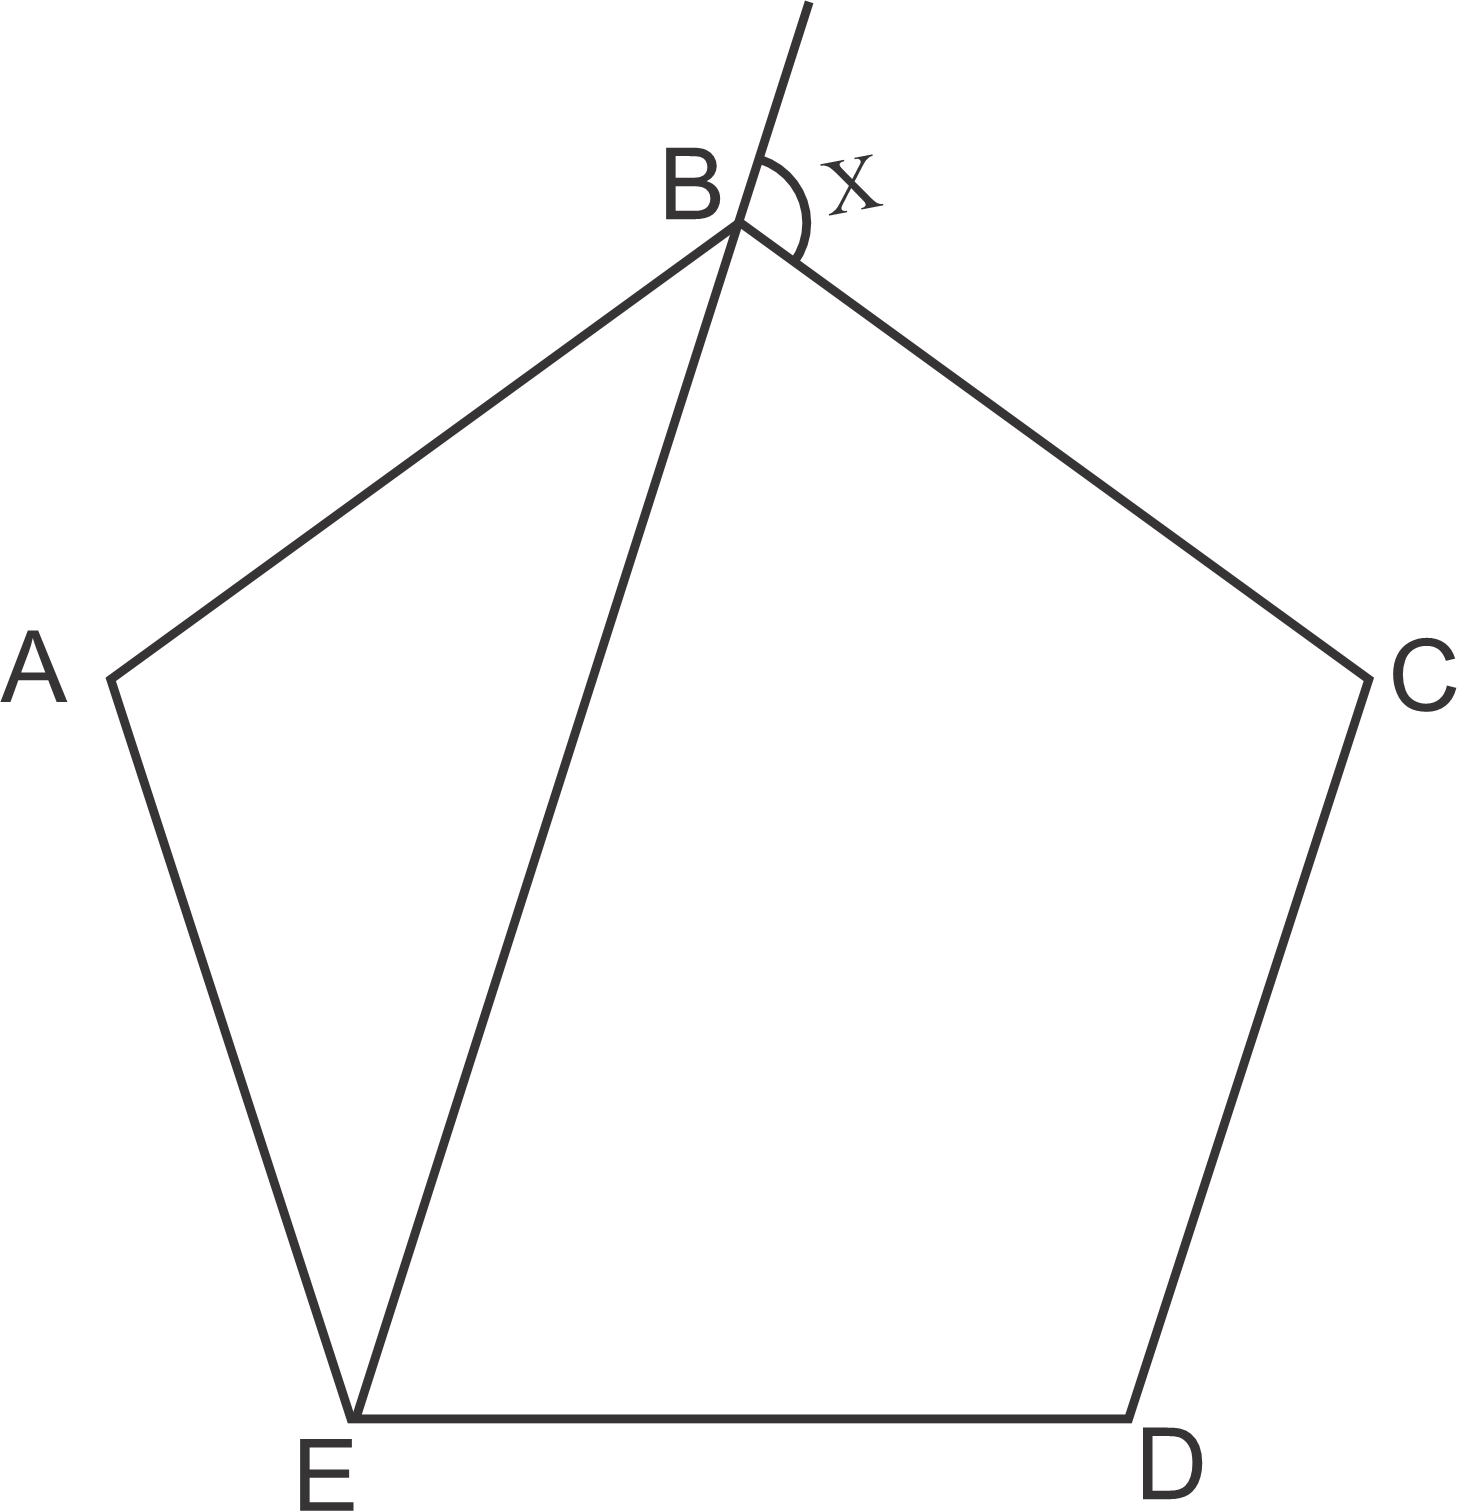
\includegraphics[width=4cm]{imagenes/general2024-I/etapa2/ing/Enunciado-1.png}\par\vspace{2cm}
	\end{center}
	\vspace{1mm}	
	\begin{enumerate}[label=\alph*)]
		\item 36°
		\item 72°
		\item 108°
		\item 120°
		\item 144°
	\end{enumerate}
	
	\textbf{Respuesta correcta:} c)
	
	\vspace{2mm}
	\textbf{Solucionario:}
	
	De la figura  se tiene
	
	$x+72^\circ=180^\circ$
	
	$x=180^\circ-72^\circ$
	
	\fbox{$x=108°$}
	
	
	\begin{center}
		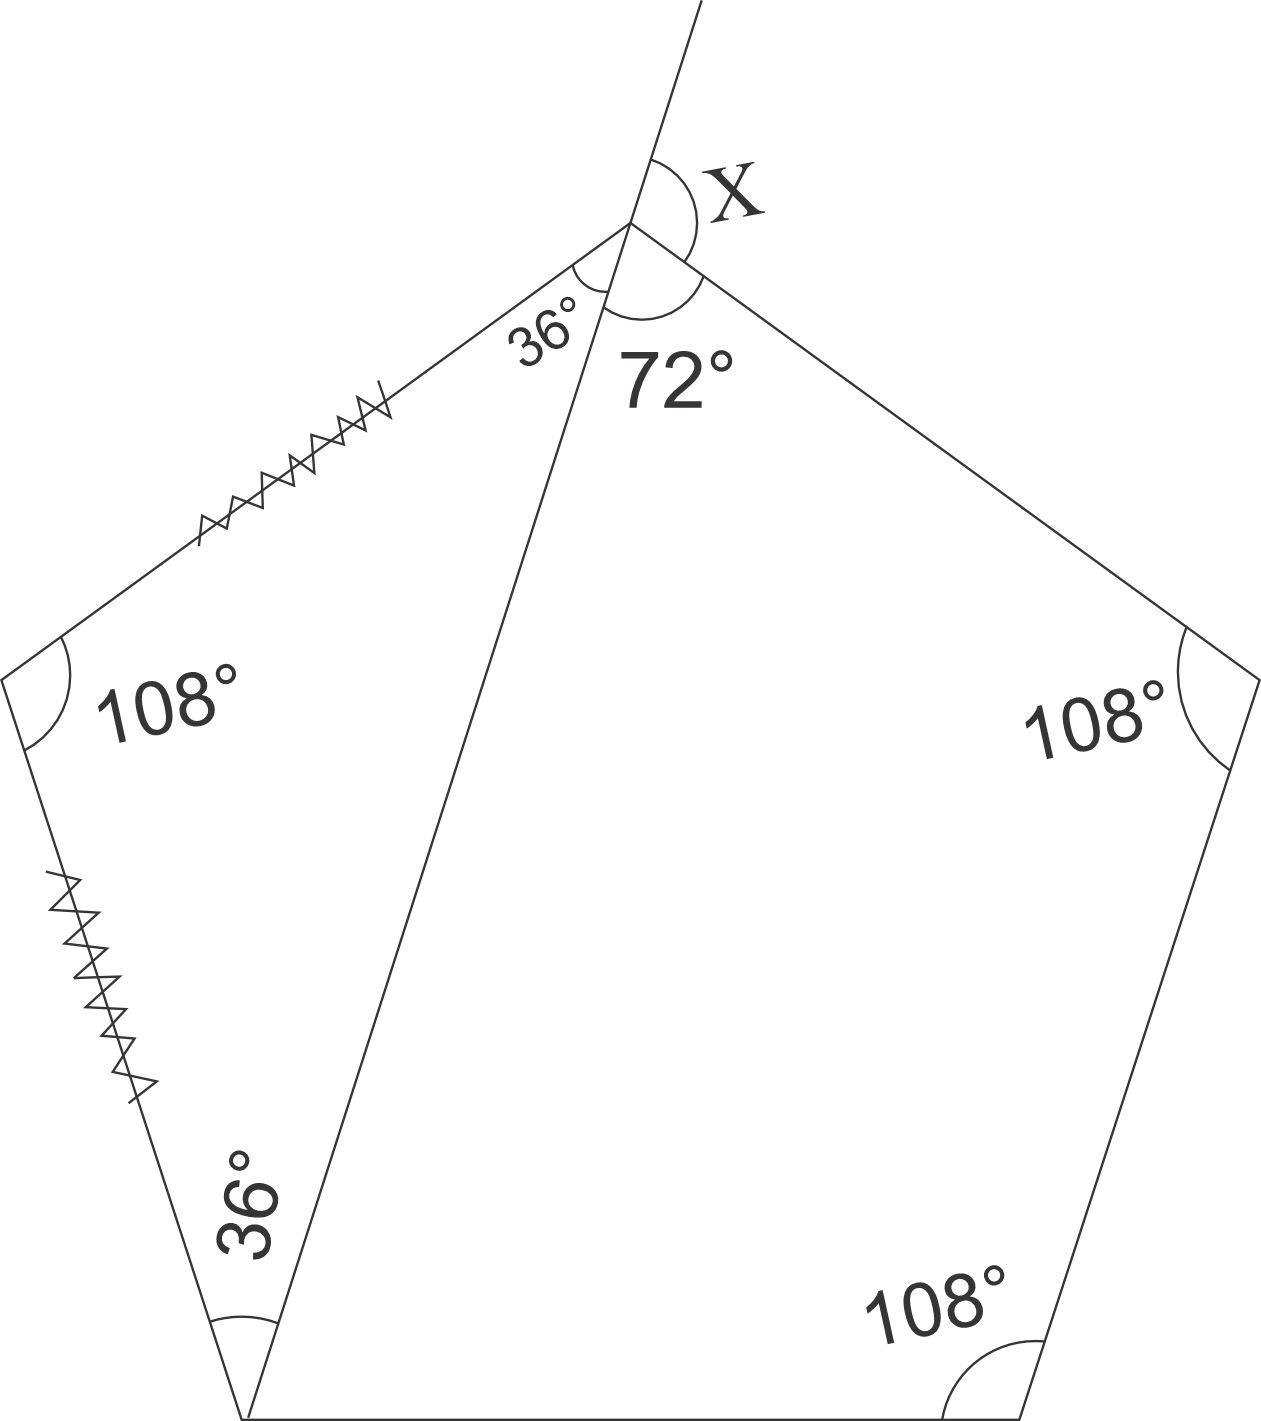
\includegraphics[width=4cm]{imagenes/general2024-I/etapa2/ing/Pgeometria1.png}\par\vspace{2cm}
	\end{center}
	
	
	\item En un cono circular recto de 9cm de altura y 15 cm de radio, se inscribe un cilindro circular recto de 5cm de radio tal que una de sus bases está sobre la base del cono. Calcule el volumen del cilindro.
	\begin{enumerate}[label=\alph*)]
		\item 120 $\pi cm^3$
		\item 130 $\pi cm^3$
		\item 140 $\pi cm^3$
		\item 150 $\pi cm^3$
		\item 160 $\pi cm^3$
	\end{enumerate}
	
	\textbf{Respuesta correcta:} d)
	
	\vspace{2mm}
	\textbf{Solucionario:}
	
	\begin{center}
		\begin{minipage}{0.45\textwidth}
			Por semejanza de triángulos:\\[0.2cm]
			$\dfrac{9-x}{9}=\dfrac{5}{15}$\\
			
			$9-x=\dfrac{9}{3}$\\
			
			$9-x=3$\\
			$x=6$\\
			$V_{cilindro}$ $= \pi r^2h$\\
			
			$=\pi (5)^2 * 6 $\\
			\fbox{$=150\pi cm^3$}
			\vspace{6mm}
		\end{minipage}
		\hfill
		\begin{minipage}{0.45\textwidth}
			\centering
			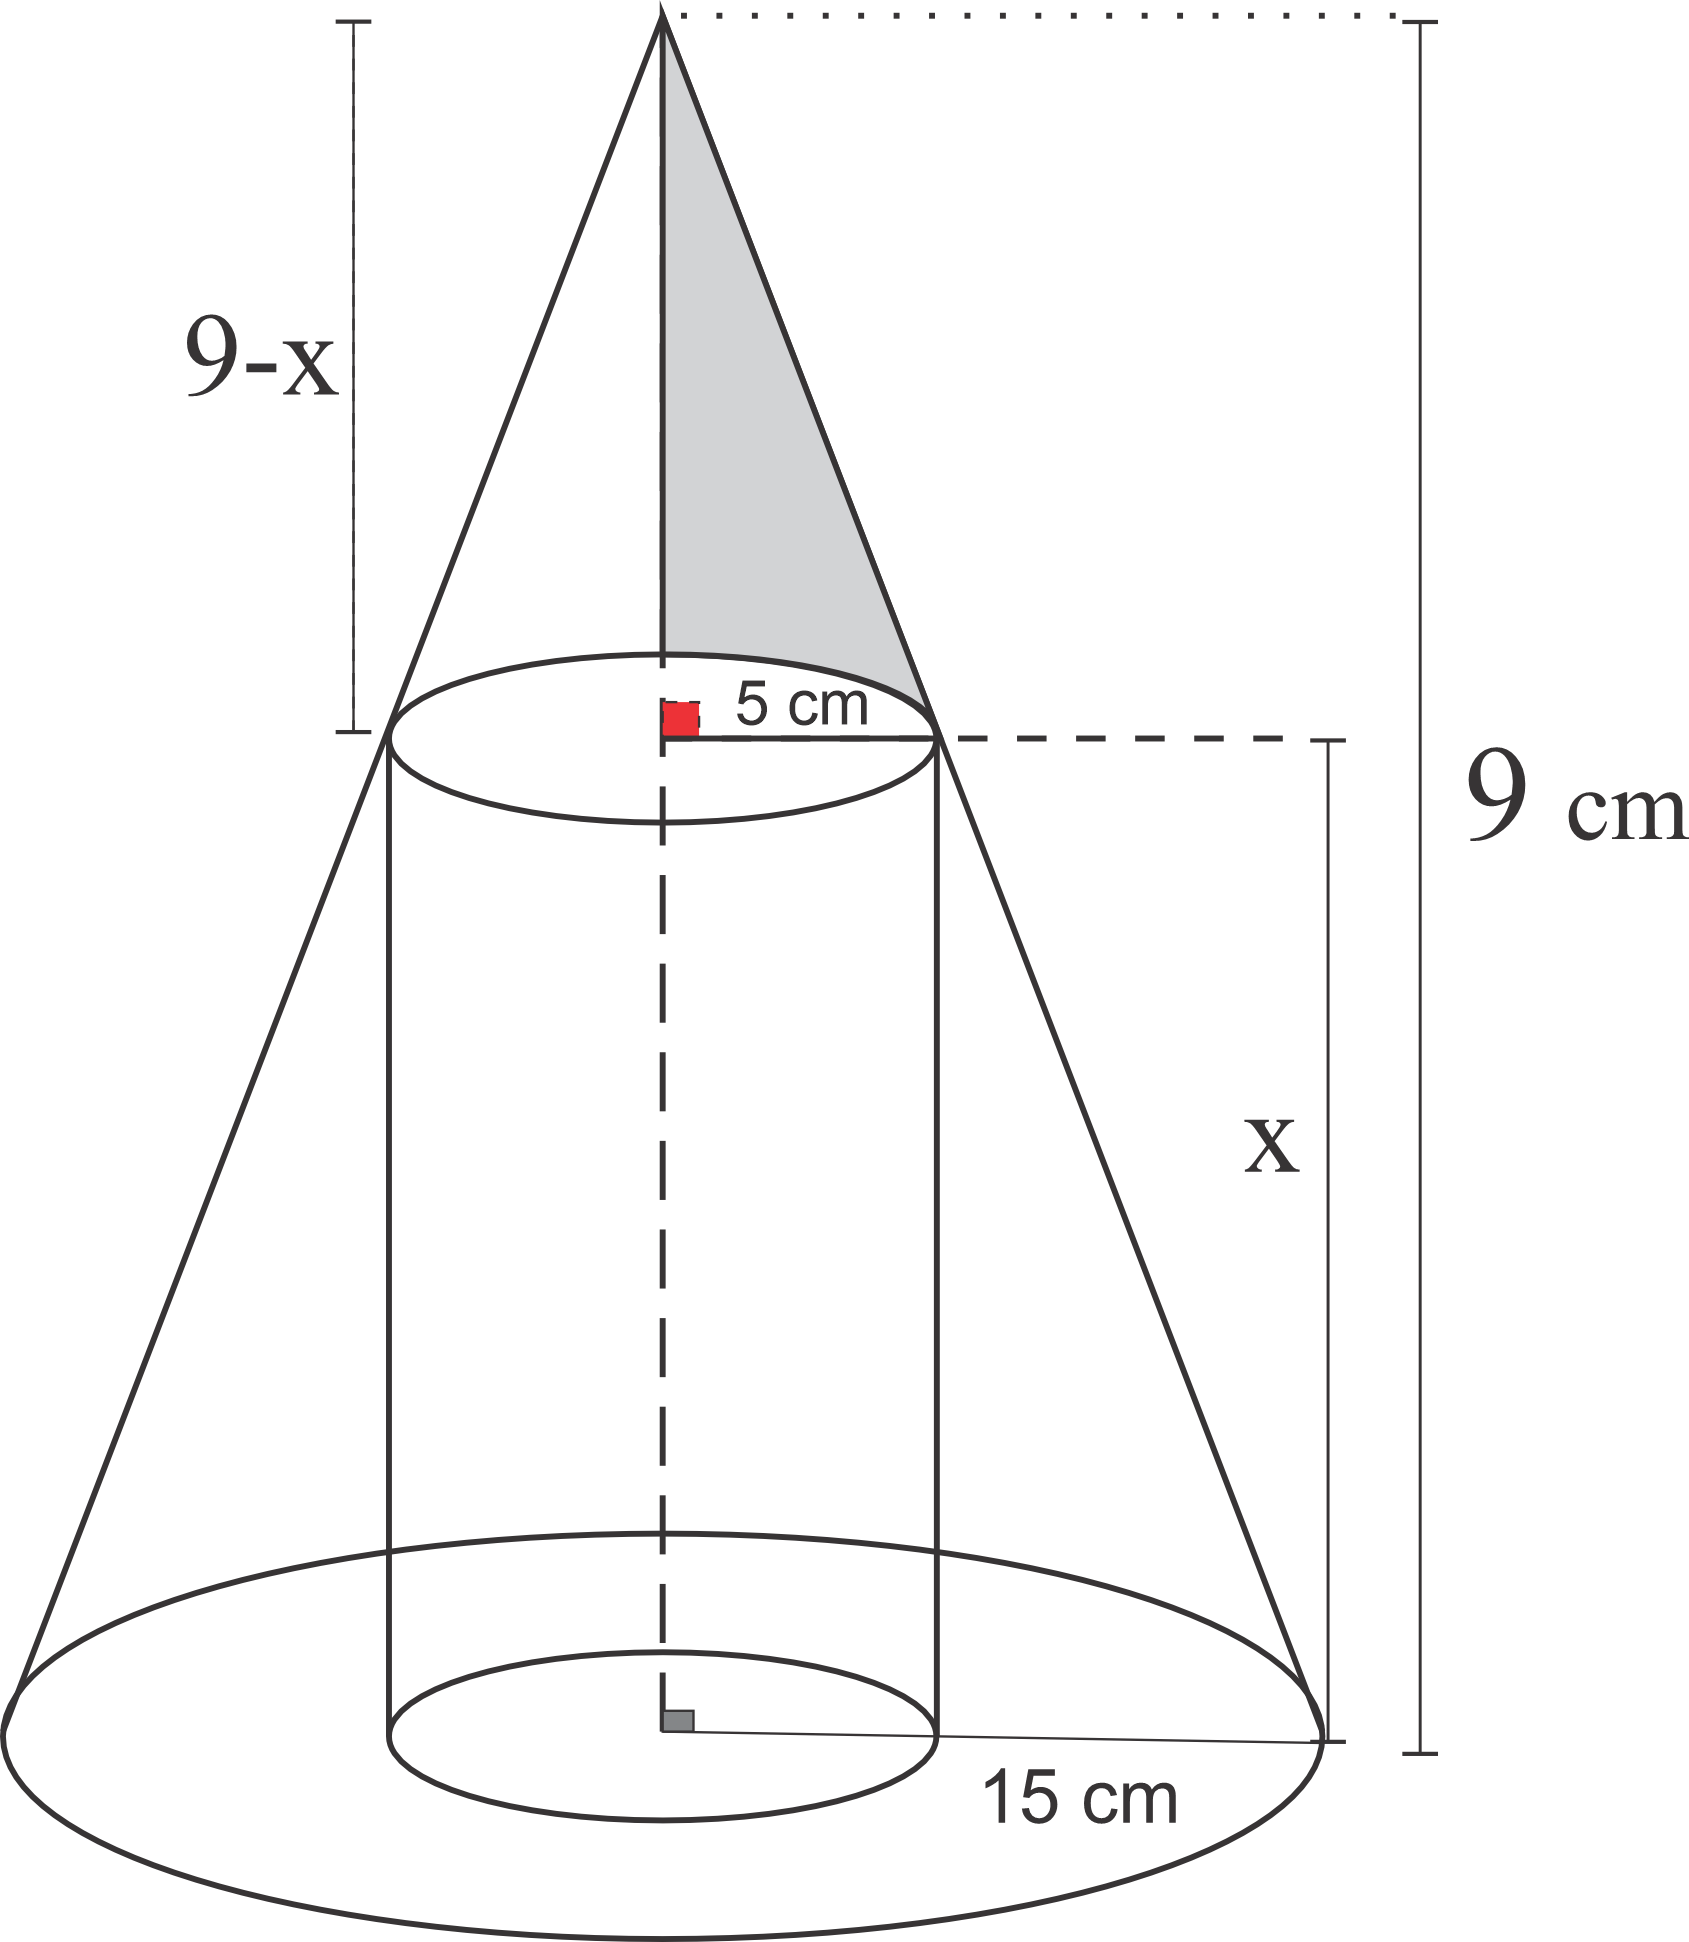
\includegraphics[width=3.5cm]{imagenes/general2024-I/etapa2/ing/problema-2.png}
		\end{minipage}
	\end{center}
	
	
	
	\item Un depósito de agua en la UNA-PUNO tiene sección transversal parabólica. Cuando el nivel del agua alcanza una altura de 18m, su ancho mide 24m.halle el ancho del nivel del agua cuando este desciende 10m. 
	\begin{enumerate}[label=\alph*)]
		\item 8 m
		\item 16 m
		\item 32 m
		\item 25 m
		\item 20 m
	\end{enumerate}
	
	\textbf{Respuesta correcta:} b)
	
	\vspace{2mm}
	\textbf{Solucionario:}

	\begin{center}
		\begin{minipage}{0.45\textwidth}
			De la fig:\\
			$\mathscr{P} : x^2=4py$
			
			$\bullet  12^2=4p(18) \longrightarrow p=2$\\
			
			$\bullet  a^2=4(2)(8) \longrightarrow  a=8$\\
			
			
			
			$\therefore$ El nuevo Ancho del agua $= 8+8=$\fbox{$16$	}
			\vspace{6mm}
		\end{minipage}
		\hfill
		\begin{minipage}{0.45\textwidth}
			\centering
			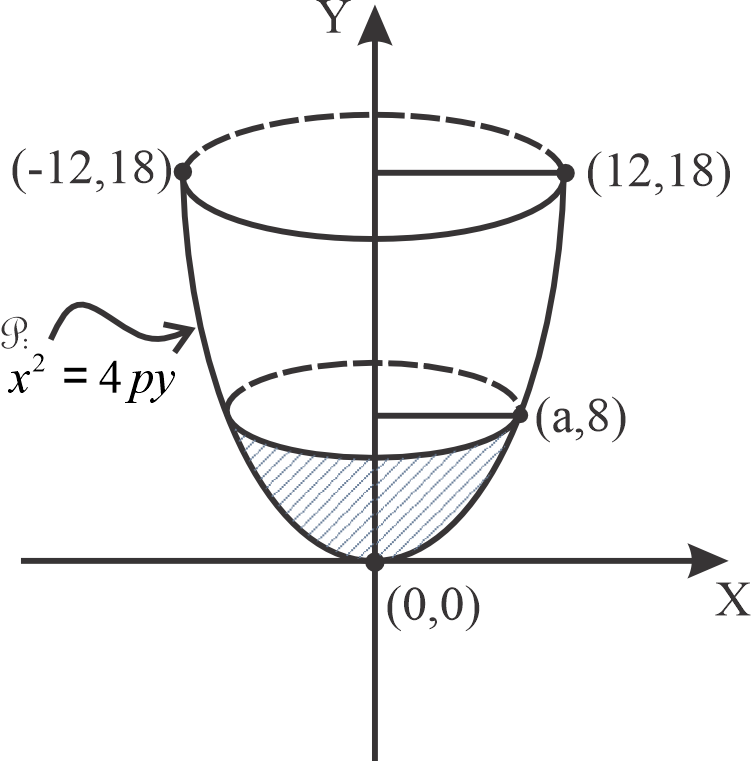
\includegraphics[width=4.3cm]{imagenes/general2024-I/etapa2/ing/problema 3 geometris.png}
		\end{minipage}
	\end{center}
	

	\vspace{6mm}
	
	\item Halle  la longitud de la figura  continua si m$\overset{\frown}{EF}
	$ es 60°y los demas arcos son semicicunferencias de igual radio.
	
	
	
	\begin{center}
		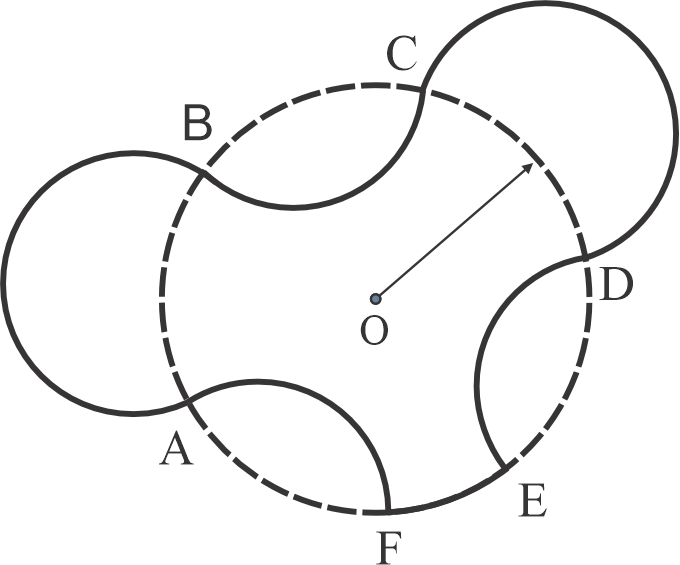
\includegraphics[width=4.3cm]{imagenes/general2024-I/etapa2/ing/probgeometria4.png}\par
		\vspace{2cm}
	\end{center}
	
	
	
	\begin{enumerate}[label=\alph*)]
		\item $\dfrac{15\pi}{2}R$
		\item $\dfrac{16\pi}{3}R$
		\item $\dfrac{17\pi}{6}R$
		\item $18\pi R$
		\item $\dfrac{19\pi}{3}R$
	\end{enumerate}
	
	\textbf{Respuesta correcta:} c)
	
	\vspace{2mm}
	\textbf{Solucionario:}
	
	$
	L_{\text{total}}
	= 5L + L_{\overset{\frown}{EF}}
	$
	
	$
	= 5(\pi r) + \dfrac{2\pi R\,\theta}{360^\circ}
	$
	
	$
	= 5\!\left(\dfrac{2\pi\left(\tfrac{R}{2}\right)}{2}\right)
	+ \dfrac{2\pi R(60^\circ)}{360^\circ}
	$
	
	$
	= \dfrac{5\pi R}{2} + \dfrac{\pi R}{3}
	$
	
	\fbox{$
	= \dfrac{17\pi R}{6}
	$}
	
	
	\vspace{6mm}
\end{enumerate}


\subsection*{Trigonometría}

\begin{enumerate}[resume]
	
	\item Un niño y dos árboles se encuentran en una misma línea. El niño que está entre los árboles observa las partes superiores de dichos árboles con ángulos de elevacion $\alpha$ y $2\alpha$. Si se sabe que sus respectivas visuales miden 30 y 35 metros,Calcule la altura del mayor árbol, temiendo en cuenta que la distancia a la que encuentra el niño de un árbol es igual a la altura del otro árbol y ese último es el que se opone a $2\alpha$.
	\begin{enumerate}[label=\alph*)]
		\item $\dfrac{60}{7}m$
		\item $\dfrac{40}{7}m$
		\item $\dfrac{60\sqrt{10}}{7}m$
		\item $\dfrac{50\sqrt{10}}{7}m$
		\item $\dfrac{45\sqrt{10}}{7}m$
	\end{enumerate}
	
	\textbf{Respuesta correcta:} b)
	
	\vspace{2mm}
	\textbf{Solucionario:}
	
	
	\begin{center}
		\begin{minipage}{0.45\textwidth}
			Igualando\\
			$35\sen2 \alpha =30\cos \alpha$\\
			
			$35(2\sen \alpha \cos\alpha)=30\cos\alpha$\\
			
			$\sen \alpha=\dfrac{3}{7}$\\
			
			$x=30$.$\cos\alpha$\\
			
			$x=30$.$\dfrac{2\sqrt{10}}{7}=$\fbox{$\dfrac{60\sqrt{10}}{7} $}
			\vspace{6mm}
		\end{minipage}
		\hfill
		\begin{minipage}{0.45\textwidth}
			\centering
			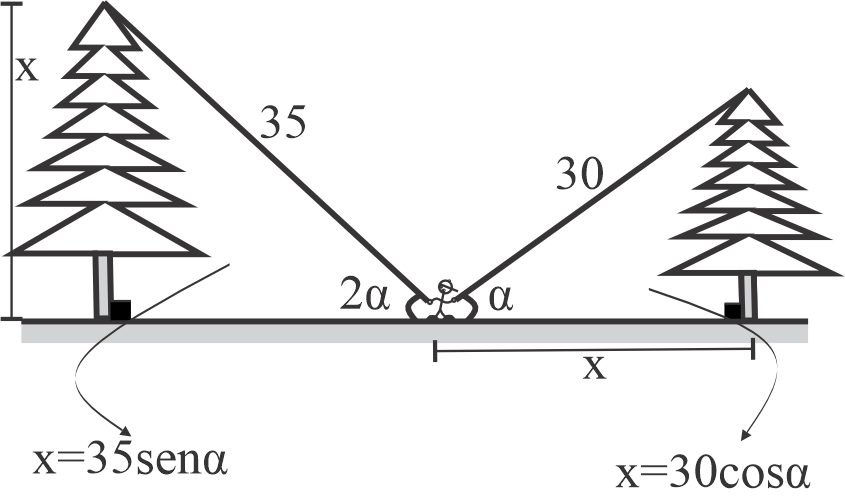
\includegraphics[width=4.5cm]{imagenes/general2024-I/etapa2/ing/trigonometria-1.png}
		\end{minipage}
	\end{center}
	
	
	
	\vspace{6mm}
	
	\item En la figula mostrada, determine $\tan$ $\theta$
	\begin{center}
		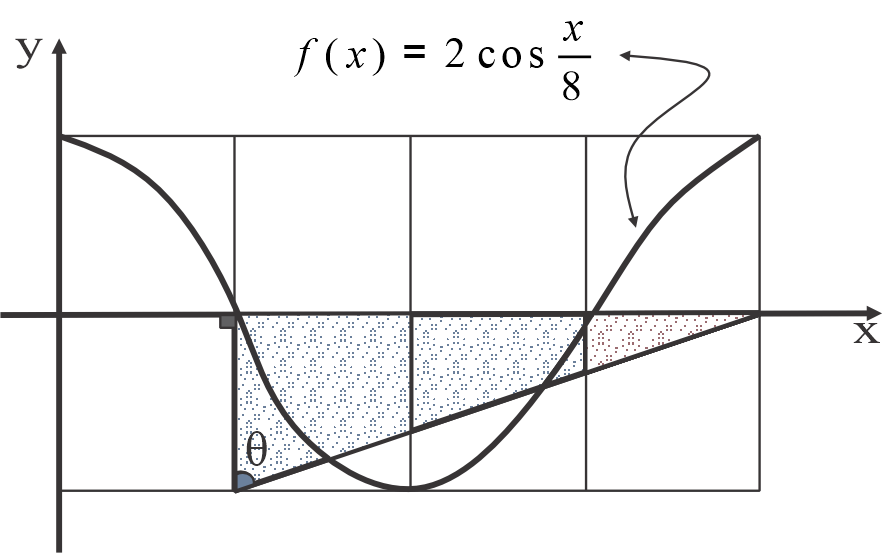
\includegraphics[width=4.8cm]{imagenes/general2024-I/etapa2/ing/trigonometria-2.png}
	\end{center}
	
	\begin{enumerate}[label=\alph*)]
		\item 5$\pi$
		\item 2$\pi$
		\item 4$\pi$
		\item 6$\pi$
		\item 3$\pi$
	\end{enumerate}
	
	\textbf{Respuesta correcta:} d)
	
	\vspace{2mm}
	\textbf{Solucionario:}
	
	\begin{center}
		\begin{minipage}{0.45\textwidth}
			$ \bigstar w=\dfrac{1}{8}$\\
			
			$\dfrac{2\pi}{T}=\dfrac{1}{8}$\\
			
			$T=16\pi $\\
			
			$\bigstar A=2$\\
			
			$\tan \theta =\dfrac{12\pi}{2}=$\fbox{$6\pi$}
			
			\vspace{6mm}
		\end{minipage}
		\hfill
		\begin{minipage}{0.45\textwidth}
			\centering
			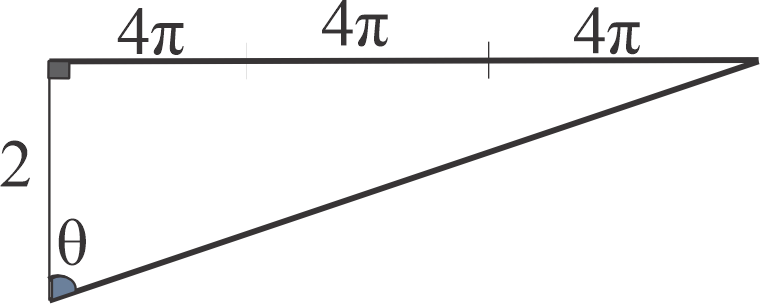
\includegraphics[width=4.5cm]{imagenes/general2024-I/etapa2/ing/trigonometria-2.2.png}
		\end{minipage}
	\end{center}

\item En el gráfico,calcular el valor de:

$M=12\cos\theta - 5 \cos\alpha.$
\begin{center}
	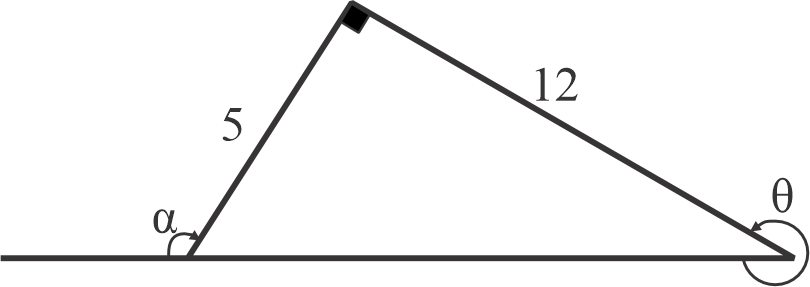
\includegraphics[width=4.5cm]{imagenes/general2024-I/etapa2/ing/trigonometria-3.png}
\end{center}


\begin{enumerate}[label=\alph*)]
	\item 26
	\item 15
	\item 11
	\item 14
	\item 13
\end{enumerate}

\textbf{Respuesta correcta:} e)

\vspace{2mm}
\textbf{Solucionario:}

	\begin{center}
	\begin{minipage}{0.45\textwidth}
		$\cos(\overbrace{360°-\theta}^{\text{$IV_c$}})=\cos\theta=\dfrac{12}{13}$\\
		$\cos(\overbrace{180°-\alpha}^{\text{$II_c$}})=-\cos\alpha=\dfrac{5}{13}$\\
		Reemplazando: \\
		$M= 12 \cos\theta-5\cos\alpha$\\
		
		$M=12(\dfrac{12}{13})-5(\dfrac{-5}{13})$\\
		
		$M=\dfrac{144+25}{13}=\dfrac{13^2}{13}=$\fbox{$13$}
		\vspace{5mm}
	\end{minipage}
	\hfill
	\begin{minipage}{0.45\textwidth}
		\centering
		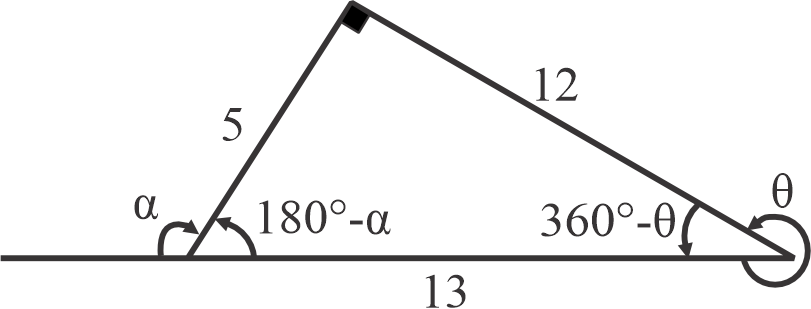
\includegraphics[width=4.5cm]{imagenes/general2024-I/etapa2/ing/trigonometria-3.3.png}
	\end{minipage}
\end{center}


\vspace{6mm}

		

	\item Determine la Variación de:\\
	
	$K= \dfrac{\sen\alpha-2}{\sen\alpha+2},\alpha \in  III_c$\\
	
\begin{enumerate}[label=\alph*)]
	\item $\langle-2;0\rangle$
	\item $\langle-3;-1\rangle$
	\item $\langle-4;-2\rangle$
	\item $\langle-3;0\rangle$
	\item $\langle-2;-1\rangle$
\end{enumerate}
\textbf{Respuesta correcta:} c)

\vspace{2mm}
\textbf{Solucionario:}

$K= \dfrac{\sen\alpha+2}{\sen\alpha+2}-\dfrac{4}{\sen\alpha+2}$

$K= 1-\dfrac{4}{\sen\alpha+2}$

$III_c \rightsquigarrow -1< \sen\alpha < 0  $

$1< \sen\alpha+2 < 2$

$1>\dfrac{1}{5\alpha+2}>\dfrac{1}{2}$

$-4<\dfrac{-4}{5\alpha+2}<-2 $

$-3<1-\dfrac{4}{5\alpha+2}<-1 $

$-3<K<-1 $

	\fbox{
$\langle-3;-1\rangle$
}
\vspace{6mm}

\end{enumerate}

\vspace{6mm}


\subsection*{Física}


\begin{enumerate}[resume]
	
	\item En la figura, se demuestra una esferaque tiene una carga de 10C y una masa de 5kg,que se encuentra en equilibrio mecánico dentro de un campo eléctrico uniforme de 5N/C, unida a una cuerda no conductora. Determine el ángulo $\theta$ que dorma la cuerda con el eje vertical.$(g=10 m/s_2)$
	\begin{enumerate}[label=\alph*)]
		\item 60°
		\item 45°
		\item 30°
		\item 53°
		\item 37°
	\end{enumerate}
	\textbf{Respuesta correcta:} b)
	
	\vspace{2mm}
	\textbf{Solucionario:}\\[1mm]
	
	
	
	
	\begin{center}
		\begin{minipage}{0.45\textwidth}
		$\sum F_x=0$\\
		
		$T\sen\theta=Eq..............I$	\\
		
		$\sum F_y=0 $\\
		
		$ T\cos\theta=mg..............II$\\
		
			\vspace{6mm}
		\end{minipage}
		\hfill
		\begin{minipage}{0.45\textwidth}
			\centering
			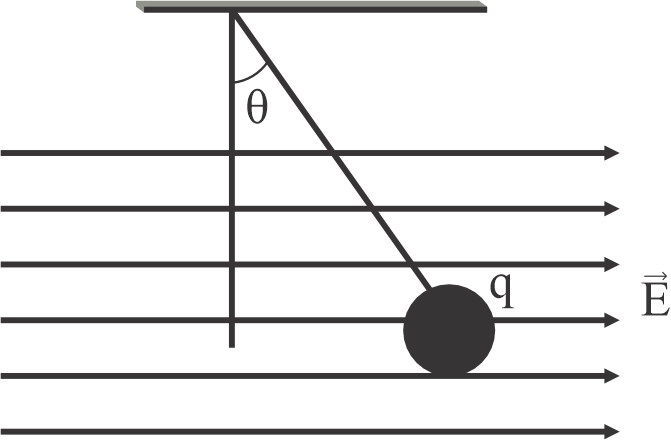
\includegraphics[width=4.5cm]{imagenes/general2024-I/etapa2/ing/fisica-1.png}
		\end{minipage}
	\end{center}
	
	
	
	\begin{center}
		\begin{minipage}{0.45\textwidth}
		$I \div II$\\
		
		$\dfrac{T\sen\theta}{T\cos\theta}=\dfrac{Eq}{mg}$\\
		
		$\tan\theta=\dfrac{(5)(10)}{(5)(10)}=1$\\
		
			\fbox{
		$\theta=45°$
	}
			\vspace{6mm}
		\end{minipage}
		\hfill
		\begin{minipage}{0.45\textwidth}
		\centering
		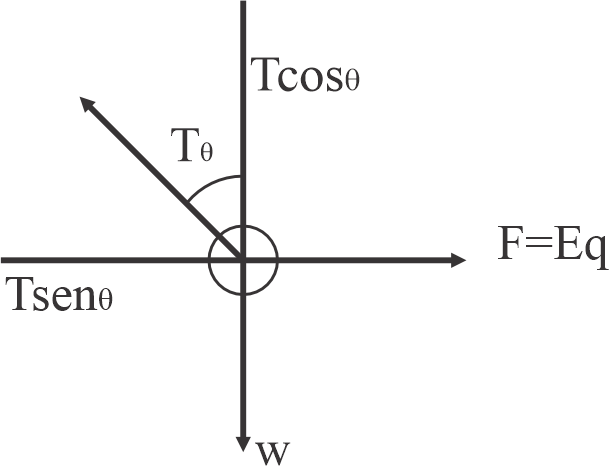
\includegraphics[width=4.5cm]{imagenes/general2024-I/etapa2/ing/fisica-1.1.png}
		\end{minipage}
	\end{center}
	
	
	
	
	
	\vspace{6mm}
	
	\item Una partícula con +3mC de carga que tiene una velocidad de $\vec{v}=(\hat{J}+2\hat{k})10^3m/s$, está dentro de un campo magnético $\vec{B}=2\hat{i}T$. Calcule la fuerza magnética sobre la partícula.
	\begin{enumerate}[label=\alph*)]
		\item $(10\hat{J}-2\hat{k})N$
		\item $(12\hat{J}-6\hat{k})N$
		\item $(12\hat{i}+ 6\hat{J})N$
		\item $(9\hat{J}-3\hat{k})N$
		\item $(8\hat{i}-5\hat{k})N$
	\end{enumerate}
	\textbf{Respuesta correcta:} b)
	
	\vspace{2mm}
	\textbf{Solucionario:}

	$q = 3 \, \text{mC} \quad ; \quad \vec{v} = \hat{J} + 2\hat{k} \cdot 10^3 \, \text{m/s}$
	\phantom{$q = 3 \, \text{mC} \quad ; \quad$} $\vec{B} = 2\hat{i} \, \text{T}$
	
	Por tanto:
	
	$\vec{F} = q \vec{v} \times \vec{B} = 3 \times 10^{-3} 
	\begin{vmatrix} 
		\hat{i} & \hat{J} & \hat{k} \\ 
		0 & 10^3 & 2 \times 10^3 \\ 
		2 & 0 & 0 
	\end{vmatrix} \text{N}$
	
	$\vec{F} = 3 \times 10^{-3} (0\hat{i} - (0 - 4 \times 10^3)\hat{J} + (0 - 2 \times 10^3)\hat{k})$
	
	$\vec{F} = 3 \times 10^{-3} (0\hat{i} + 4 \times 10^3\hat{J} - 2 \times 10^3\hat{k})$
	
	\fbox{
		$\vec{F} = (12\hat{J} - 6\hat{k}) \, \text{N}$
	}
	
	\vspace{6mm}
	
		\item La frecuencia de un fotón ultravioleta es $6 \times 10^{15} \, \text{Hz}$. Calcule la cantidad de movimiento del fotón. ($h = 6,63 \times 10^{-34} \, \text{J}\cdot\text{s}$)
	\begin{enumerate}[label=\alph*)]
		\item $8,23\times10^{-27} kg. m/s$
		\item $9,27\times10^{-25} kg. m/s$
		\item $10,21\times10^{-26} kg. m/s$
		\item $11,20\times10^{-27} kg. m/s$
		\item $13,26\times10^{-27} kg. m/s$
	\end{enumerate}
	\textbf{Respuesta correcta:} e)
	
	\vspace{2mm}
	\textbf{Solucionario:}
	
	$P = \dfrac{h}{\lambda} = \dfrac{hf}{c}$
	
	$P = \dfrac{(6,63 \times 10^{-34} \, \text{J}\cdot\text{s})(6 \times 10^{15} \, \text{Hz})}{3 \times 10^8 \, \text{m/s}}$
	
	$P = 6,63 \times 10^{-34} \times 2 \times 10^{15} \times 10^{-8}$
	
	\fbox{
	$P = 13,26 \times 10^{-27} \, \text{kg}\cdot\text{m/s}$
}
	\vspace{6mm}
	
	\item Una función de onda transversal está dada por $\psi(x,t)=20\cos(\dfrac{\pi}{8}x-6\pi t)$ donde $x$ y $\psi$ están en centímetros, $t$ en segundos. Calcule la rapidez de propagación y el periodo de oscilación.
	\begin{enumerate}[label=\alph*)]
		\item $30 cm/s ; 2s.$
		\item $48 cm/s ; \dfrac{1}{3}s.$
		\item $40 cm/s ; \dfrac{1}{4}s.$
		\item $24 cm/s ; \dfrac{1}{3}s.$
		\item $20 cm/s ; 1s.$
	\end{enumerate}
	\textbf{Respuesta correcta:} b)
	
	\vspace{2mm}
	\textbf{Solucionario:}
	
		$\psi = A \cos(kx - \omega t)$
		
		$\phantom{\psi} = 20 \cos\left(\dfrac{\pi}{8}x - 6\pi t\right)$
		
		\fbox{$A = 20 \, \text{cm}$}
		
		$k = \dfrac{\pi}{8} \, \text{cm}^{-1}$
		
		$\omega = 6\pi \, \text{rad/s}$
		
		$v = \dfrac{\omega}{k} = \dfrac{6\pi \, \text{rad/s}}{\dfrac{\pi}{8} \, \text{cm}^{-1}} = 48 \, \text{cm/s}$
		
		$T = \dfrac{2\pi}{\omega} = \dfrac{2\pi}{6\pi} =$ \fbox{$ \dfrac{1}{3} \, \text{s}$}
	
	\vspace{6mm}	
	
	
	
	
	
	
	
	
	
	
	
	
	
\end{enumerate}


\subsection*{Química}

\begin{enumerate}[resume]
	
	\item Se dispone de gas helio a 2400 mmHg contenido en un recipiente cúbico. Si dicho gas se traslada a otro cubo cuya arista es la cuarta parte de la arista del primero y su temperatura se reduce en un 60\%, ¿cuál será su presión final en mmHg?
	\begin{enumerate}[label=\alph*)]
		\item 75000
		\item 61440
		\item 64040
		\item 60440
		\item 76000
	\end{enumerate}
	\textbf{Respuesta correcta:} b)
	
	\vspace{2mm}
	\textbf{Solucionario:}\\[1mm]
	
	
		\begin{center}
		\begin{minipage}{0.45\textwidth}
		\centering
		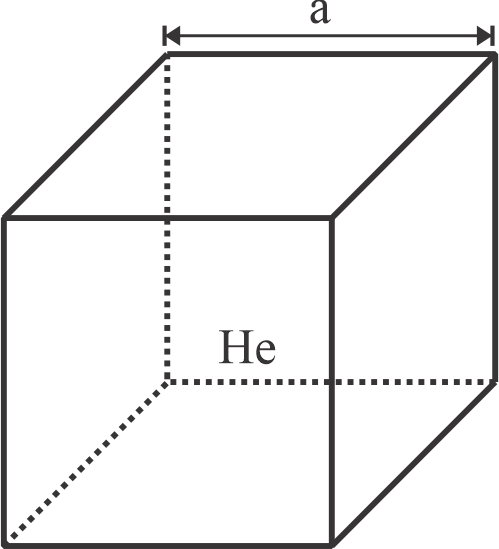
\includegraphics[width=3.5cm]{imagenes/general2024-I/etapa2/ing/quimica-1.png}
		\vspace{6mm}
		\end{minipage}
		\hfill
		\begin{minipage}{0.45\textwidth}
			\centering
			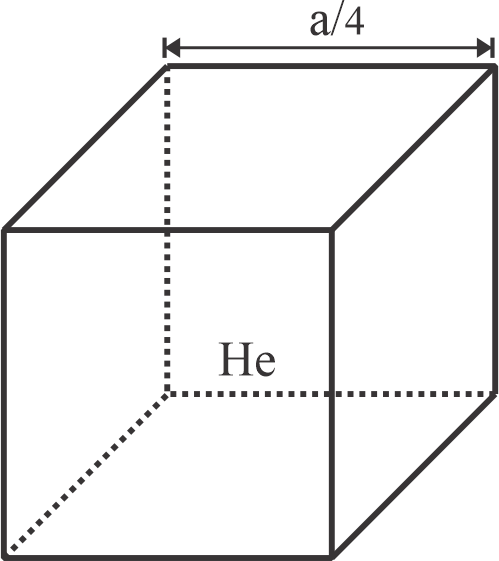
\includegraphics[width=2cm]{imagenes/general2024-I/etapa2/ing/quimica-1.1.png}
		\end{minipage}
	\end{center}
	
	
	
	\begin{center}
		\begin{minipage}{0.45\textwidth}
				
			$V_1 = a^3$ 
			
			$P_1 = 2400$ 
			
			$T_1 = T$
			\vspace{6mm}
		\end{minipage}
		\hfill
		\begin{minipage}{0.45\textwidth}
			$V_2 = \left(\dfrac{a}{4}\right)^3$\\
			$P_2 = ?$\\
			$T_2 = 0,4T$
		\end{minipage}
	\end{center}
	
	
	Utilizamos la ecuación general de los gases ideales:
	
	$\dfrac{P_1 V_1}{T_1} = \dfrac{P_2 V_2}{T_2}$
	
	$\dfrac{(2400)(a^3)}{T} = \dfrac{P_2 \cdot \left(\dfrac{a}{4}\right)^3}{0,4T}$
	
	$\Rightarrow (0,4T)(2400)(a^3) = \dfrac{P_2 (a^3) T}{64}$
	
	$\Rightarrow$ \fbox{ $P_2 = 61440 \, \text{mm Hg}$}
	
	\vspace{6mm}
	
	\item ¿Cuántos segundos debe transcurrir para que una corriente de $120 \, \text{A}$ deposite en el cátodo $5 \, \text{g}$ de hierro ($\text{Fe}$) de una solución de cloruro de hierro(III), $\text{FeCl}_3$?
	
	($1 \, \text{Faraday} = 96\,500 \, \text{Coulomb} \quad ; \quad \text{PA}(\text{Fe}) = 56$)
	\begin{enumerate}[label=\alph*)]
		\item 25,4
		\item 235,5
		\item 96,5
		\item 215,4
		\item 155,4
	\end{enumerate}
	\textbf{Respuesta correcta:} d)
	
	\vspace{2mm}
	\textbf{Solucionario:}\\
	
	Datos\\
	$I = 120 \, \text{A}$
	
	$t = ?$
	
	$m = 5 \, \text{g}$
	
	$\text{PA Fe} = 56$
	
	$\text{Farad} = 96\,500 \, \text{coulombios}$
	
	$\Rightarrow$ Utilizando ley de Faraday
	
	
	$m = \dfrac{P_{eq} \cdot I \cdot t}{96\,500}$ , despejando tiempo $t = \dfrac{96\,500 \cdot m}{P_{eq} \cdot I}$
	
	
	$t = \dfrac{(96\,500)(5)}{\left( \dfrac{56}{3} \right) \cdot 120}$ $\Rightarrow$ \fbox{$ t = 215,4 \, \text{s}$}
	

	\item ¿Qué masa de óxido de calcio se obtendrá si se calcina 1 tonelada de caliza, cuyo contenido de $C_aCO_3$ es del $62\%?  (C_a = 40;C=12;O=16)$\\
	$C_aCO_{3(s)}+calor \Rightarrow  C_aO_{(s)}+CO_{2(g)}$
	
	\begin{enumerate}[label=\alph*)]
		\item 347,2
		\item 233,4
		\item 374,0
		\item 185,8
		\item 620,0
	\end{enumerate}
	
	\textbf{Respuesta correcta:} a)
	
	\vspace{2mm}
	\textbf{Solucionario:}
	
	\textbf{Datos}
	
	$M_{CaO} = ?$
	
	Pureza $CaCO_3 = 62\%$
	
	1 Tonelada = $1000 \, kg$
	
	$ PM \, CaCO_3 = 100$
	
	$PM \, CaO = 56$
	
	Si la caliza tiene una pureza de $62\%$, entonces:\\
	$CaCO_3 = 1000 \, kg \times 62\%$\\
	$CaCO_3 = 620 \, kg$ puro\\
	
	$\Rightarrow \quad CaCO_3 \xrightarrow{\hspace{1cm}} CaO$\\
	\phantom{$\Rightarrow \quad$} $100 \xrightarrow{\hspace{1cm}} 56$\\
	\phantom{$\Rightarrow \quad$} $620 \xrightarrow{\hspace{1cm}} X$\\

	$X = \dfrac{(620)(56)}{100}$\\
	
	\fbox{
		$X = 347,2 \, g \, CaO$
	}
	
	
	\item Señale la suma de coeficientes de los productos en la siguiente reacción química:
	
	$CrI_3 + Cl_2 + KOH \rightarrow KIO_4 + K_2CrO_4 + KCl + H_2O$
	
	\begin{enumerate}[label=\alph*)]
		\item 65
		\item 46
		\item 39
		\item 94
		\item 87
	\end{enumerate}
	\textbf{Respuesta correcta:} d)
	
	\vspace{2mm}
	\textbf{Solucionario:}
	
	Asignamos estados de oxidación:
	
	En $CrI_3$:
	
	$Cr=+3$
	
	$I=-1$
	
	En $KIO_4$:
	
	$I+4(-2)+1=0$
	
	$I-8+1=0$
	
	$I=+7$
	
	En $K_2CrO_4$:
	
	$Cr+4(-2)+2(+1)=0$
	
	$Cr-8+2=0$
	
	$Cr=+6$
	
	
	$Cr^{+3}\rightarrow Cr^{+6}$
	
	Pierde $3e^-$
	
	$I^{-1}\rightarrow I^{+7}$
	
	Pierde $8e^-$
	
	$Cl_2^{0}\rightarrow Cl^{-1}$
	
	Gana $2e^-$
	
	
	$2CrI_3+27Cl_2+64KOH\rightarrow 6KIO_4+2K_2CrO_4+54KCl+32H_2O$
	
	La suma de coeficientes de los productos es:
	
	$6+2+54+32=94$
	
	\fbox{$94$}
	
	\vspace{6mm}
	
	
	
	
\end{enumerate}	
	
	
	
	\subsection*{Biología y Anatomía}
	
	\begin{enumerate}[resume]
		
		\item las plantas que crecen cerca del agua y en suelos muy húmedos con provisión de agua permanente, como los musgos y helechos se denominan:
		
		\begin{enumerate}[label=\alph*)]
			\item halofitas.
			\item psicrofitas.
			\item higrófitas.
			\item xenófitas.
			\item hidrofitas.
		\end{enumerate}
		
		\textbf{Respuesta correcta:} c)
		
	\vspace{2mm}
	\textbf{Solucionario:}\\[1mm]
	
	Las higrófitas son plantas que se desarrollan en ambientes con alta humedad y con disponibilidad permanente de agua, como riberas, pantanos y suelos constantemente húmedos. Ejemplos típicos son los musgos y helechos, los cuales requieren condiciones húmedas para su crecimiento y reproducción.
	No viven totalmente sumergidas, a diferencia de las hidrófitas.
		
		\vspace{6mm}
		
		\item Son peces vertebrados sin mandíbulas, carecen de escamas y tienen una piel mucosa resbaladiza.
		\begin{enumerate}[label=\alph*)]
			\item Condrictios
			\item Gnatostomados
			\item Osteíctios
			\item Tunicados
			\item Agnatos
		\end{enumerate}
		
		\textbf{Respuesta correcta:} e)
		
			\vspace{2mm}
		\textbf{Solucionario:}
		
		Los agnatos son vertebrados primitivos caracterizados por carecer de mandíbulas, escamas y aletas pares. Presentan una piel mucosa resbaladiza y una boca circular adaptada para succión. Ejemplos representativos son las lampreas y mixinos, considerados los peces más antiguos.
		
		\vspace{6mm}
		
	\end{enumerate}
	

\subsection*{Psicología y Filosofía}

\begin{enumerate}[resume]
	
	\item Claudia le dice a su mamá: ¡La ropa de caperucita es muy bonita!, mientras esta le lee el cuento.
	¿Qué tipo de imaginación está utilizando Claudia?
	
	\begin{enumerate}[label=\alph*)]
		\item Creadora
		\item Reproductora
		\item Icónica
		\item Alucinación
		\item Fantástica
	\end{enumerate}
	
	\textbf{Respuesta correcta:} b)
	
      \vspace{2mm}
      \textbf{Solucionario:}\\
      
      La imaginación reproductora consiste en recrear mentalmente imágenes ya conocidas, a partir de relatos, lecturas o experiencias previas.
      Claudia imagina la vestimenta de Caperucita Roja basándose en el cuento que está escuchando, sin crear elementos nuevos, por lo que no se trata de una imaginación creadora o fantástica.
	
	\vspace{6mm}
	
	\item Rebeca le dice a su hijo: "Cuando termines la tarea te llevaré al cine. En el acto, Rebeca, para controlar el comportamiento de su hijo, utiliza el:
	\begin{enumerate}[label=\alph*)]
		\item reforzamiento positivo.
		\item castigo negativo.
		\item castigo positivo.
		\item reforzamiento continuo.
		\item reforzamiento negativo.
	\end{enumerate}
	
	\textbf{Respuesta correcta:} a)
	

	\vspace{2mm}
	\textbf{Solucionario:}\\
	
 El reforzamiento positivo consiste en presentar un estímulo agradable (ir al cine) para incrementar una conducta deseada (hacer la tarea).
 Rebeca motiva a su hijo ofreciéndole una recompensa, lo cual aumenta la probabilidad de que cumpla con la tarea.
	
	
	
	\item El escéptico \underline{\hspace{1.5cm}} la posibilidad del conocimiento pleno.
	
	\begin{enumerate}[label=\alph*)]
		\item afirma
		\item niega
		\item prueba
		\item comprueba
		\item critica
	\end{enumerate}
	
	\textbf{Respuesta correcta:} b)
	
	
	\vspace{2mm}
	\textbf{Solucionario:}\\
	
	El escepticismo es una corriente filosófica que niega o duda de la posibilidad de alcanzar un conocimiento verdadero y absoluto.
	El escéptico sostiene que el ser humano no puede conocer la realidad de manera plena y definitiva, por lo que adopta una actitud de duda constante.


	\vspace{6mm}
	
	\item Es el conocimiento práctico de las cosas, basado en la experiencia personal, arbitrario y carente de fundamentación.
	\begin{enumerate}[label=\alph*)]
		\item conocimiento filosófico
		\item conocimiento científico
		\item conocimiento vulgar
		\item conocimiento conceptual
		\item conocimiento metafisíco
	\end{enumerate}
	
	\textbf{Respuesta correcta:} c)
		
		
		\vspace{2mm}
		\textbf{Solucionario:}\\
	
		El conocimiento vulgar (o empírico) es aquel que se adquiere a través de la experiencia cotidiana, sin método ni fundamentación científica.
		Es subjetivo, asistemático y arbitrario, pero útil para la vida diaria, ya que permite desenvolverse en situaciones comunes.
		
		
	\vspace{6mm}
		
\end{enumerate}





\subsection*{Geografía}

\begin{enumerate}[resume]
	
	\item De acuerdo al MINAM, ¿qué instrumento técnico se requiere para desarrollar el ordenamiento territorial?
	
	\begin{enumerate}[label=\alph*)]
		\item La estrategia global para la sostenibilidad
		\item La Zonificación Ecológica y Económica
		\item El estudio no especializado
		\item El levantamiento topográfico
		\item La caracterización de imágenes satelitales
	\end{enumerate}
	
	\textbf{Respuesta correcta:} b)
	
	\vspace{2mm}
	\textbf{Solucionario:}\\[1mm]
	El Ministerio del Ambiente (MINAM) establece que la Zonificación Ecológica y Económica (ZEE) es el principal instrumento técnico para el ordenamiento territorial.
	La ZEE permite identificar las potencialidades y limitaciones del territorio, considerando criterios físicos, biológicos, sociales, económicos y culturales, con el fin de orientar el uso sostenible del territorio y la toma de decisiones públicas y privadas.
	
	\vspace{6mm}
	
	\item En el Perú, \dots\dots\dots\dots\dots son áreas destinadas a la conservación de la diversidad biológica y a la utilización sostenible de los recursos de flora y fauna silvestre, con excepción de la explotación forestal comercial, en el marco de la clasificación de áreas naturales protegidas (ANP)
	\begin{enumerate}[label=\alph*)]
		\item los Parques nacionales
		\item los Bosques de protección
		\item las Reservas comunales
		\item las Reservas nacionales
		\item las Zonas reservadas
	\end{enumerate}
	
	\textbf{Respuesta correcta:} d)
	
		\vspace{2mm}
	\textbf{Solucionario:}\\[1mm]
	En el Perú, las Reservas Nacionales son un tipo de Área Natural Protegida (ANP) destinadas a la conservación de la diversidad biológica, donde se permite el aprovechamiento sostenible de los recursos naturales, excepto la explotación forestal maderable comercial.
	Estas actividades deben realizarse bajo planes de manejo y supervisión del Estado, garantizando la sostenibilidad de los ecosistemas.
	
	\vspace{6mm}
	
\end{enumerate}



\subsection*{Historia}

\begin{enumerate}[resume]
	
\item Para realizar cálculos matemáticos, los incas utilizaron un instrumento denominado:

\begin{enumerate}[label=\alph*)]
	\item tocapu.
	\item quipu.
	\item yupana.
	\item ushnu.
	\item urpo.
\end{enumerate}

\textbf{Respuesta correcta:} c)

\vspace{2mm}
\textbf{Solucionario:}\\[1mm]
La yupana era un dispositivo utilizado por los incas (una especie de ábaco) para realizar operaciones aritméticas complejas. Aunque el quipu se usaba para la contabilidad y registro de datos, la yupana era la herramienta específica para el cálculo.

\vspace{6mm}

\item La cultura romana exaltó los triunfos a través de monumentos arquitectónicos conocidos como:

\begin{enumerate}[label=\alph*)]
	\item esculturas.
	\item pórticos.
	\item obeliscos.
	\item arcos.
	\item columnas.
\end{enumerate}

\textbf{Respuesta correcta:} d)

\vspace{2mm}
\textbf{Solucionario:}\\[1mm]
Los Arcos de Triunfo eran estructuras monumentales construidas por los romanos para conmemorar victorias militares y honrar a sus generales o emperadores.


	
	\vspace{6mm}
	
\end{enumerate}


\subsection*{Educación Cívica}

\begin{enumerate}[resume]
	

	\vspace{2mm}	

	\item Es el responsable de velar por el mantenimiento de la moral pública, perseguir y prevenir el delito y promover la reparación civil en favor de las personas que son lesionadas en sus derechos e intereses.
	
	\begin{enumerate}[label=\alph*)]
		\item Tribunal Constitucional
		\item Ministerio Público
		\item Fuerzas Armadas
		\item Poder Judicial
		\item Poder Ejecutivo
	\end{enumerate}
	
	\textbf{Respuesta correcta:} b)
	
	\vspace{2mm}
	\textbf{Solucionario:}\\[1mm]
	El Ministerio Público es el organismo autónomo del Estado que tiene como funciones principales la defensa de la legalidad y de los intereses públicos tutelados por el derecho, así como la persecución del delito y la reparación civil de las víctimas.
	
	\vspace{6mm}
	
	\item El Secretario General de la OEA y la ONU son elegidos por un periodo de:
	
	\begin{enumerate}[label=\alph*)]
		\item cuatro y cinco años respectivamente.
		\item cinco y cuatro años respectivamente.
		\item cinco años para cada Secretario General.
		\item cuatro años para cada Secretario con posibilidad de reelección.
		\item cuatro años sin posibilidad de reelección.
	\end{enumerate}
	
	\textbf{Respuesta correcta:} c)
	
	\vspace{2mm}
	\textbf{Solucionario:}\\[1mm]
	
	Tanto el Secretario General de la Organización de los Estados Americanos (OEA) como el de la Organización de las Naciones Unidas (ONU) son elegidos para ejercer sus funciones por un periodo de cinco años.

	
	\vspace{6mm}
	
\end{enumerate}


\subsection*{Economía}

\begin{enumerate}[resume]
	
\item En una economía de mercado, si la inflación subió en forma inesperada por encima de lo proyectado; entonces, los salarios se \underline{\hspace{2cm}} y los beneficios se \underline{\hspace{2cm}}.

\begin{enumerate}[label=\alph*)]
	\item incrementan - reducen.
	\item indexan - distribuyen.
	\item reducen - incrementan.
	\item reducen - reducen.
	\item incrementan - incrementan.
\end{enumerate}

\textbf{Respuesta correcta:} d)

\vspace{2mm}
\textbf{Solucionario:}\\[1mm]

En un escenario de inflación inesperada, los salarios reales se reducen porque pierden poder adquisitivo frente al alza de precios. Asimismo, los beneficios reales de las empresas también pueden verse reducidos debido a la incertidumbre económica, el aumento en los costos de los insumos y la caída en la demanda real de los consumidores.

\vspace{6mm}

\item En un determinado mercado, las funciones de demanda y oferta para una mercancía son:
\[ Q_x^d = 40 - 0,7Px \]
\[ Q_x^s = 10 + 0,3Px \]

Al precio de S/ 10 cada uno, se puede afirmar que en el mercado:

\begin{enumerate}[label=\alph*)]
	\item abunda la mercadería.
	\item sobran 10 unidades.
	\item faltan 20 unidades.
	\item sobran 30 unidades.
	\item faltan 40 unidades.
\end{enumerate}

\textbf{Respuesta correcta:} c)

\vspace{2mm}
\textbf{Solucionario:}\\[1mm]
Reemplazamos el precio ($Px = 10$) en ambas funciones:
\begin{itemize}
	\item Cantidad demandada: $Q_d = 40 - 0,7(10) = 40 - 7 = 33$
	\item Cantidad ofertada: $Q_s = 10 + 0,3(10) = 10 + 3 = 13$
\end{itemize}
Como la demanda ($33$) es mayor que la oferta ($13$), existe un exceso de demanda de $33 - 13 = 20$ unidades. Por lo tanto, faltan 20 unidades.


\vspace{6mm}
	
\end{enumerate}



\subsection*{Comunicación}

\begin{enumerate}[resume]
	
\item Escuché la voz de mi padre diciéndome "Mira Jaime ese es el Capitán", mientras señalaba al jugador que llevaba un brazalete al lado derecho.

En el fragmento, predomina el texto:

\begin{enumerate}[label=\alph*)]
	\item instructivo.
	\item descriptivo.
	\item narrativo.
	\item argumentativo.
	\item expositivo.
\end{enumerate}

\textbf{Respuesta correcta:} c)

\vspace{2mm}
\textbf{Solucionario:}\\[1mm]
El texto es narrativo porque relata un suceso o acción en un tiempo y espacio determinados (la acción de escuchar al padre y observar al jugador), presentando una secuencia de hechos.

\vspace{6mm}

\item Los sustantivos que nombran seres reales que pueden ser percibidos por nuestros sentidos y, por tanto, ser tocados, vistos, medidos, se denominan:

\begin{enumerate}[label=\alph*)]
	\item Propios.
	\item Concretos.
	\item Abstractos.
	\item Individuales.
	\item Colectivos.
\end{enumerate}

\textbf{Respuesta correcta:} b)

\vspace{2mm}
\textbf{Solucionario:}\\[1mm]
Los sustantivos concretos designan objetos o seres que tienen existencia física y real, los cuales pueden ser captados a través de los sentidos (vista, tacto, oído, etc.).

\vspace{6mm}

\item Como actuar en caso de accidente de tránsito:\\
1.- Cubra con ropas al lesionado para mantener su temperatura.\\
2.- Prevenga el shock.\\
3.- Controle la hemorragia, si la hay.\\
4.- Asegúrese de que el herido se mantenga respirando.

El propósito comunicativo del texto es:

\begin{enumerate}[label=\alph*)]
	\item advertir.
	\item convencer.
	\item deleitar.
	\item informar.
	\item mostrar.
\end{enumerate}

\textbf{Respuesta correcta:} a)

\vspace{2mm}
\textbf{Solucionario:}\\[1mm]
El texto tiene una función apelativa o exhortativa; su propósito es advertir y dar pautas de comportamiento o instrucciones necesarias para actuar ante una situación de emergencia.

\vspace{6mm}

\item Una obra literaria, en el proceso comunicativo, constituye el:

\begin{enumerate}[label=\alph*)]
	\item emisor.
	\item mensaje.
	\item código.
	\item receptor.
	\item contexto.
\end{enumerate}

\textbf{Respuesta correcta:} b)

\vspace{2mm}
\textbf{Solucionario:}\\[1mm]
Dentro del proceso de comunicación, la obra literaria es el contenido o la información que el autor (emisor) transmite al lector (receptor), por lo tanto, constituye el mensaje.

\vspace{6mm}
	
\end{enumerate}


\subsection*{Literatura}

\begin{enumerate}[resume]

\item Escribió poemas bajo el título \textit{Rimas}, 22 leyendas y una colección de prosas con el título \textit{Cartas desde mi Celda}.

\begin{enumerate}[label=\alph*)]
	\item Miguel de Cervantes Saavedra
	\item Tirso de Molina
	\item Francisco de Quevedo
	\item Gustavo Adolfo Bécquer
	\item Pedro Calderón de la Barca
\end{enumerate}

\textbf{Respuesta correcta:} d)

\vspace{2mm}
\textbf{Solucionario:}\\[1mm]

Gustavo Adolfo Bécquer es la figura máxima del Romanticismo tardío español. Su fama reside principalmente en sus \textit{Rimas}, poemas breves de tono melancólico, y sus \textit{Leyendas}, narraciones fantásticas en prosa. Escribió \textit{Cartas desde mi celda} durante su estancia en el monasterio de Veruela.

\vspace{6mm}

\item Mariátegui, a diferencia de otros intelectuales, consideró que al problema del indio era de carácter:

\begin{enumerate}[label=\alph*)]
	\item religioso
	\item educativo
	\item económico
	\item político
	\item moral
\end{enumerate}

\textbf{Respuesta correcta:} c)

\vspace{2mm}
\textbf{Solucionario:}\\[1mm]
En sus \textit{7 ensayos de interpretación de la realidad peruana}, José Carlos Mariátegui sostiene que el problema del indio no es pedagógico, moral ni jurídico, sino que tiene raíces económicas vinculadas a la propiedad de la tierra (el problema agrario y el gamonalismo).

\vspace{6mm}


\end{enumerate}






\subsection*{Razonamiento Matemático}

\begin{enumerate}[resume]



\item Si la suma de las fechas de todos los viernes de un determinado mes es igual a 85, ¿qué día cae el 15 de dicho mes?

\begin{enumerate}[label=\alph*)]
	\item Martes
	\item Miércoles
	\item Jueves
	\item Viernes
	\item Lunes
\end{enumerate}

\textbf{Respuesta correcta:} b)

\vspace{2mm}
\textbf{Solucionario:}

Las fechas de un mismo día de la semana forman una progresión aritmética de razón 7:

sea el primer viernes $= a$

 $a, a+7, a+14, a+21, a+28$.
 
Si sumamos 5 viernes: 

$5a + 70 = 85 \Rightarrow 5a = 15 \Rightarrow a = 3$.

Los viernes son: 3, 10, 17, 24 y 31.

Si el viernes es 17, retrocedemos dos días para llegar al 15: el día es miercoles.

\vspace{6mm}

\item Pamela con todas las monedas que tiene, forma un arreglo triangular de la siguiente manera: en la primera fila 1 moneda, en la segunda fila 2 monedas y sobre cada una de ellas una más, en la tercera fila tres monedas y sobre cada una de ellas 2 monedas más y así sucesivamente. Si pudo formar 20 filas en total, ¿cuántas monedas tenía?

\begin{enumerate}[label=\alph*)]
	\item 2790
	\item 2890
	\item 2870
	\item 2320
	\item 5740
\end{enumerate}

\textbf{Respuesta correcta:} c)

\vspace{2mm}
\textbf{Solucionario:}

Número de monedas por fila ($f$):

Fila 1: $1 \times 1 = 1^2$

Fila 2: $2 \times 2 = 2^2$

Fila 3: $3 \times 3 = 3^2$

Total para 20 filas:

$\sum_{i=1}^{20} i^2 = \dfrac{n(n+1)(2n+1)}{6}$

$S = \dfrac{20(21)(41)}{6} = 10(7)(41) = $\fbox{$2870$ monedas.}

\vspace{6mm}


\item Se compra un televisor en 630 soles. ¿Cuánto debo aumentar a este precio para que durante la venta se realice una rebaja de 10\% y así gane el 40\% del precio de costo?

\begin{enumerate}[label=\alph*)]
	\item S/ 250
	\item S/ 252
	\item S/ 350
	\item S/ 98
	\item S/ 198
\end{enumerate}

\textbf{Respuesta correcta:} c)

\vspace{2mm}
\textbf{Solucionario:}\\[1mm]
Sea $10x$ el aumento total sobre el costo. La rebaja es el $10\%$ de este aumento, es decir, $x$.
\begin{itemize}
	\item Precio de costo ($P_c$) = S/ 630
	\item Ganancia esperada ($40\% P_c$) = $0,40 \times 630$ = S/ 252
	\item Dinero a recibir = $P_c + \text{Ganancia} = 630 + 252 = 882$
\end{itemize}
Si el aumento total es $10x$ y se rebaja $x$, el dinero recibido equivale a $9x$:\\
$9x = 882 \Rightarrow x = 98$.\\
El costo a incrementar total es la Ganancia + Rebaja: $252 + 98 = \text{S/ 350}$.\\

\vspace{6mm}

\vspace{6mm}
\item Sabiendo que $\overline{UNA} + \overline{ANU} = 988$ y $U - A = 4$, calcule $N + A$.

\begin{enumerate}[label=\alph*)]
	\item 10
	\item 14
	\item 11
	\item 13
	\item 18
\end{enumerate}

\textbf{Respuesta correcta:} c)

\vspace{2mm}
\textbf{Solucionario:}

De la suma en unidades: $A + U = 8$.

Como $U - A = 4$, sumamos ambas: $(A+U) + (U-A) = 8 + 4 \Rightarrow 2U = 12 \Rightarrow U=6$.

Entonces $A = 2$.

En las decenas: $N + N = 18 \Rightarrow 2N = 18 \Rightarrow N = 9$.

Piden $N + A = 9 + 2 = 11$.

\vspace{6mm}

	\item En el cuadrado ABCD, cuyo lado mide 4 cm, determine el área de la región sombreada, siendo O el centro de la circunferencia.
	
		\begin{center}
		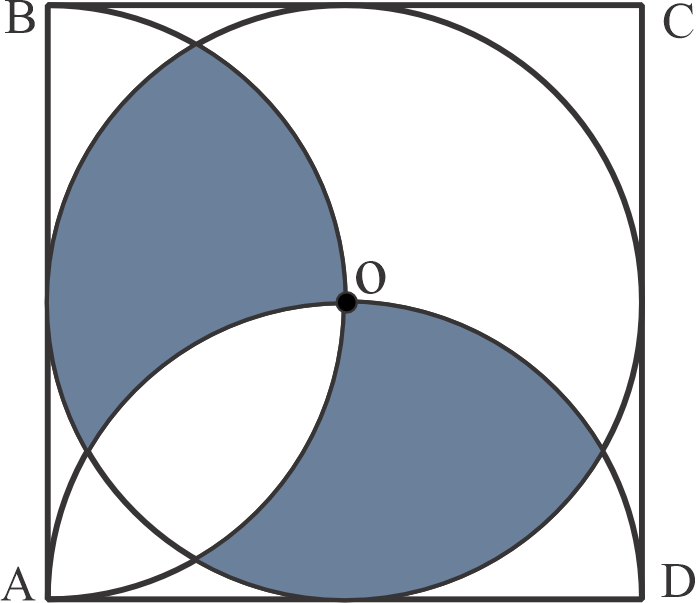
\includegraphics[width=3.5cm]{imagenes/general2024-I/etapa2/ing/rm5.png}\par\vspace{2cm}
	\end{center}
	
	
	
\begin{enumerate}[label=\alph*)]
	\item 4,0 \( \pi cm^2\)
	\item 3,5 \( \pi cm^2\)
	\item 3,0 \( \pi cm^2\)
	\item 2,5 \( \pi cm^2\)
	\item 2,0 \( \pi cm^2\)
\end{enumerate}

\textbf{Respuesta correcta:} e)

\vspace{2mm}
\textbf{Solucionario:}

	\begin{center}
	\begin{minipage}{0.45\textwidth}
	Al trazar $\overline{OM}$ y $\overline{ON}$, se observan regiones equivalentes, a cuyas áreas les asignamos los valores $a$ y $b$.\\
	piden $A_{somb}=2a+2b=??$\\
	Pero, del gráfico, $a+b=A_{DOND}=\dfrac{\pi 2^2}{4}=\pi\,cm^2$.\\
	$\therefore\ A_{somb}=2(a+b)=2\pi\,cm^2$\\

		\vspace{6mm}
	\end{minipage}
	\hfill
	\begin{minipage}{0.45\textwidth}
		\centering
		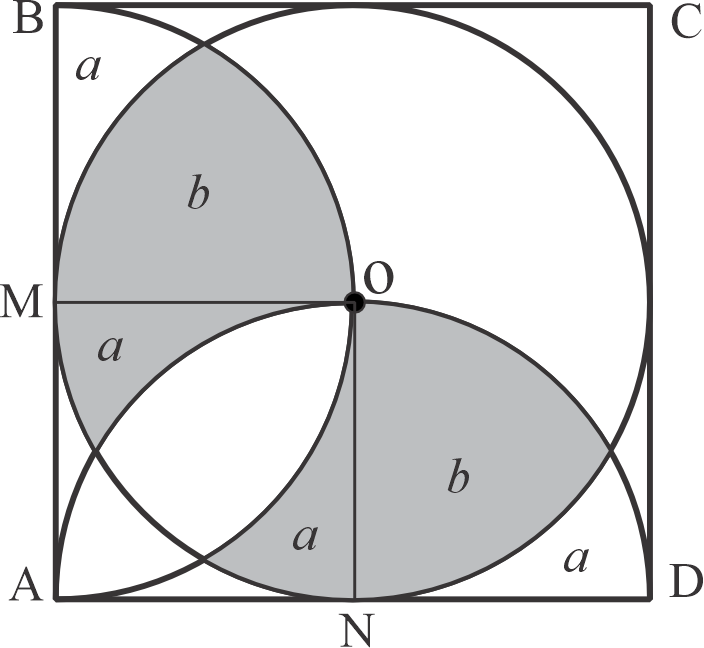
\includegraphics[width=3.5cm]{imagenes/general2024-I/etapa2/ing/rrm5.png}
	\end{minipage}
	\end{center}

\vspace{5mm}

\item El segundo término de una progresión aritmética es 7 y el séptimo término es 22. Halle la suma de los 100 primeros términos de la progresión.

\begin{enumerate}[label=\alph*)]
	\item 14250
	\item 15250
	\item 14350
	\item 15350
	\item 13250
\end{enumerate}

\textbf{Respuesta correcta:} b)

\vspace{2mm}
\textbf{Solucionario:}
$a_7 = a_2 + 5r \Rightarrow 22 = 7 + 5r \Rightarrow r = 3$.

Hallamos $a_1$: $a_2 = a_1 + r \Rightarrow 7 = a_1 + 3 \Rightarrow a_1 = 4$.

Hallamos $a_{100}$: $a_{100} = 4 + 99(3) = 301$.

Suma: $S_{100} = \dfrac{(4 + 301)100}{2} = 305 \times 50 = 15250$.



\end{enumerate}




\subsection*{Razonamiento Verbal}

\begin{enumerate}[resume]
	
\item El término que no corresponde a la palabra PARAFRASEAR es:

\begin{enumerate}[label=\alph*)]
	\item comentar.
	\item agilizar.
	\item argumentar.
	\item explicar.
	\item interpretar.
\end{enumerate}

\textbf{Respuesta correcta:} b)

\vspace{2mm}
\textbf{Solucionario:}\\[1mm]
Parafrasear consiste en explicar o interpretar un texto con palabras propias para hacerlo más comprensible. Términos como comentar, argumentar o explicar están ligados a este proceso cognitivo; sin embargo, "\text{agilizar}" no guarda relación semántica con la acción de traducir o explicar un contenido.

\vspace{6mm}

\item El sinónimo de la palabra PERORATA es:

\begin{enumerate}[label=\alph*)]
	\item discursivo.
	\item exordio.
	\item explicación.
	\item doctrina.
	\item alusión.
\end{enumerate}

\textbf{Respuesta correcta:} a)

\vspace{2mm}
\textbf{Solucionario:}\\[1mm]
Una perorata es un discurso o razonamiento, generalmente largo y aburrido, que se pronuncia ante un público. Por ello, el término \textbf{discursivo} es el que más se aproxima a la naturaleza de la palabra, aunque habitualmente se utiliza el sustantivo "discurso".

\vspace{6mm}

\item Complete las oraciones.\\
A partir de la fabricación de la primera bomba atómica, \dots\dots\dots\dots\dots se ha hecho para salvar al mundo de la guerra, \dots\dots\dots\dots\dots se ha hecho mucho \dots\dots\dots\dots\dots aumentar su capacidad destructiva.

\begin{enumerate}[label=\alph*)]
	\item poco - y - al
	\item no - y tampoco - para
	\item algo - y - como para
	\item mucho - por el contrario - con el fin de
	\item nada - mientras - para
\end{enumerate}

\textbf{Respuesta correcta:} e)

\vspace{2mm}
\textbf{Solucionario:}\\[1mm]

La oración expresa una oposición temporal y de sentido entre dos acciones relacionadas con la bomba atómica.
En la primera parte, se indica que no se ha hecho nada para salvar al mundo de la guerra; mientras que en la segunda parte se señala que sí se ha actuado con un propósito, es decir, para aumentar su capacidad destructiva.

El conector “mientras” introduce un contraste simultáneo, mostrando que, al mismo tiempo que no se realizan acciones para la paz, se desarrollan acciones orientadas a la destrucción.
La preposición “para” expresa finalidad, indicando el objetivo de aumentar el poder destructivo.

Por ello, la alternativa que mantiene coherencia lógica y semántica es:

\vspace{6mm}

\item Identifica el par analógico.\\
INGENIERO : MINA ::

\begin{enumerate}[label=\alph*)]
	\item aviador : cosmos.
	\item peregrino : agua.
	\item citadino : campo.
	\item marino : lago.
	\item geólogo : montaña.
\end{enumerate}

\textbf{Respuesta correcta:} e)

\vspace{2mm}
\textbf{Solucionario:}\\[1mm]
La analogía es de Sujeto : Lugar de trabajo o acción. Un ingeniero desempeña sus funciones técnicas frecuentemente en una mina; del mismo modo, un geólogo realiza sus estudios de campo y análisis profesional predominantemente en la montaña.
	
	
	
	\item \textbf{PLAN DE REDACCIÓN}
	
	\begin{center}
		\textbf{Los Trenes}
	\end{center}
	
	I. El Ferrocarril Central del Perú es la línea férrea más alta del mundo y fue construido en 1873. \\
	II. La empresa Nacional de Ferrocarriles del Perú fue privatizada en 1996. \\
	III. El gobierno de Velasco Alvarado crea la Empresa Nacional de Ferrocarriles (ENAFER). \\
	IV. El primer tren del Perú se inauguró en 1852, fue el Lima – Callao y luego el Lima – Chorrillos. \\
	V. En los años veinte las carreteras desplazaron a los trenes en el Perú.
	
	\begin{enumerate}[label=\alph*)]
		\item IV - I - V - III - II
		\item IV - V - I - II - III
		\item III - V - I - IV - II
		\item I - IV - V - II - III
		\item I - V - II - III - IV
	\end{enumerate}
	
	\textbf{Respuesta correcta:} a)
	
	\vspace{2mm}
	\textbf{Solucionario:}\\[1mm]
	El criterio de ordenación es cronológico:\\
	1. (IV) 1852: Primer tren.\\
	2. (I) 1873: Ferrocarril Central.\\
	3. (V) Años veinte: Desplazamiento por carreteras.\\
	4. (III) Gobierno de Velasco (1968-1975): Creación de ENAFER.\\
	5. (II) 1996: Privatización.\\	
	
	
	\item La República del Perú es democrática, social, independiente y soberana. El Estado es uno e indivisible. Su gobierno es unitario representativo y descentralizado, y se organiza según el principio de la separación de poderes (Art. 43º C.P. 93).
	
	Lo descrito significa que:
	
	\begin{enumerate}[label=\alph*)]
		\item La Constitución Política tiene un carácter presidencialista.
		\item El Congreso de la República es el primer poder del Estado.
		\item Ningún poder del Estado tiene primacía sobre el otro.
		\item El equilibrio de poderes, parcialmente está garantizado.
		\item La hegemonía del Estado de Derecho está por encima de toda ley.
	\end{enumerate}
	
	\textbf{Respuesta correcta:} c)
	
	\vspace{2mm}
	\textbf{Solucionario:}\\[1mm]
	El principio de separación de poderes establece una estructura de "frenos y contrapesos" donde el Poder Ejecutivo, Legislativo y Judicial son autónomos e independientes entre sí. Esto garantiza que no exista una jerarquía de supremacía de un poder sobre los demás, buscando el equilibrio en el ejercicio del poder estatal.
	
	
	
	\vspace{6mm}
	
	
	
	\vspace{6mm}
	
\end{enumerate}




\subsection*{Inglés}

\begin{enumerate}[resume]

\item In the sentence: Lionel Messi is a famous soccer player.
What is the underlined word?

\begin{enumerate}[label=\alph*)]
	\item a verb.
	\item a preposition.
	\item a gerund.
	\item a noun.
	\item an adjective.
\end{enumerate}

\textbf{Respuesta correcta:} e)

\vspace{2mm}
\textbf{Solucionario:}\\[1mm]
La palabra "famous" (famoso) funciona como un adjetivo en la oración, ya que su función es calificar o describir una característica del sustantivo "soccer player".

\vspace{6mm}

\item If I say: just every Monday I do the laundry.
How often do I do the laundry?

\begin{enumerate}[label=\alph*)]
	\item twice a day
	\item once a week
	\item once a day
	\item ever Friday
	\item three times a day
\end{enumerate}

\textbf{Respuesta correcta:} b)

\vspace{2mm}
\textbf{Solucionario:}\\[1mm]
La expresión "every Monday" (cada lunes) indica una frecuencia semanal. Dado que el lunes ocurre una vez por semana, la respuesta correcta es "once a week".

\vspace{6mm}
\end{enumerate}





\subsection*{Quechua y Aimara}

\begin{enumerate}[resume]



\item ¿Hayk'a k'uchukunayuqtaq wasi punkuri kan? / ¿Qawqha k'uchukananisa uta punkuxa?

\begin{enumerate}[label=\alph*)]
	\item Iskay k'uchukunayuq / Pä k'uchukananiwa.
	\item Qanchis k'uchukunayuq / Paqallqu k'uchukananiwa.
	\item Kimsa k'uchukunayuq / Kimsa k'uchukananiwa.
	\item Tawa k'uchukunayuq / Pusi k'uchukananiwa.
	\item Pichqa k'uchukunayuq / Phisqa k'uchukananiwa.
\end{enumerate}

\textbf{Respuesta correcta:} d)

\vspace{2mm}
\textbf{Solucionario:}\\[1mm]
La pregunta inquiere cuántas esquinas o ángulos tiene la puerta de una casa. Al ser rectangular, la respuesta es cuatro: \textbf{Tawa} (quechua) / \textbf{Pusi} (aymara).

\vspace{6mm}

\item ¿Ima yupaytaq chunka tawayuq chawpinri? / ¿Kuna jakhusa tunka pusini chikatapaxa?

\begin{enumerate}[label=\alph*)]
	\item Suqta / Suxta
	\item Qanchis / Paqallqu
	\item Pusaq / Kimsaqallqu
	\item Isqun / Llatunka
	\item Chunka / Tunka
\end{enumerate}

\textbf{Respuesta correcta:} b)

\vspace{2mm}
\textbf{Solucionario:}\\[1mm]
Se pregunta por la mitad de catorce (chunka tawayuq / tunka pusini). La mitad es siete: \textbf{Qanchis} en quechua y \textbf{Paqallqu} en aymara.



\end{enumerate}










\section*{Área: Biomédicas}

\addcontentsline{toc}{subsection}{Área: Biomédicas}

\subsection*{Aritmética}

\begin{enumerate}
	
	\item Una familia está dedicada a la crianza de animales y ellos tienen $\overline{aba}$ animales. A causa de una epidemia se le mueren $\overline{ab}$ vacas, $\overline{10a}$ carneros y $\overline{b0}$ conejos, hasta que al final se quedan con $\overline{7(3a)}$ animales. Halle $5a-2b$.
	\begin{enumerate}[label=\alph*)]
		\item 0
		\item -3
		\item 5
		\item 2
		\item -1
	\end{enumerate}
	\textbf{Respuesta correcta:} d)
	
	\vspace{2mm}
	\textbf{Solucionario:}
	

	$\underbrace{\overline{aba}}_{\text{Total inicial}} - \underbrace{(\overline{ab} + \overline{10a} + \overline{b0})}_{\text{mueren}} = \underbrace{\overline{7(3a)}}_{\text{Total final}}$ 
	
	Como $3a \le 9$, entonces, $1 \le a \le 3$ 
	
	Descomponemos polinómicamente: 
	
	$100a + 10b + a - (10a + b + 100 + a + 10b) = 70 + 3a$ 
	
	$100a - 10a - b - 100 = 70 + 3a$ 
	
	$87a = 170 + b$; $b < 9$ 
	
	$\downarrow$ \hspace{6mm} $\downarrow$ 
	
	$2$ \hspace{7.5mm} $4$ 
	
	Luego $5a - 2b \implies 5(2) - 2(4) = 10 - 8 =$\fbox{$ 2$}
	
	\vspace{6mm}
	
	\item Tres ciclistas parten al mismo tiempo de un punto de una pista circular que tiene $240\text{ m}$ de circunferencia. El primero con velocidad de $8\text{ m/s}$, el segundo a $5\text{ m/s}$ y el tercero a $3\text{ m/s}$. ¿Cuánto tiempo transcurrirá para que los tres móviles realicen el primer encuentro?
	\begin{enumerate}[label=\alph*)]
		\item 8 min
		\item 2 min
		\item 4 min
		\item 10 min
		\item 12 min
	\end{enumerate}
	\textbf{Respuesta correcta:} c)
	
	\vspace{2mm}
	\textbf{Solucionario:}
	
	Calculamos el tiempo que emplea c/u en dar 1 vuelta: 
	
	$T_{1ro} = 240 \div 8 = 30\text{ s}$ 
	
	$T_{2do} = 240 \div 5 = 48\text{ s}$ 
	
	$T_{3ro} = 240 \div 3 = 80\text{ s}$ 
	
	El tiempo que emplean para encontrarse por primera vez deberá ser el: 
	
	$\text{MCM}(30, 48, 80) = 240\text{ s}$ 
	
	$240\text{ s} \implies $\fbox{$4\text{ min}$}
	
	\vspace{6mm}
	
	\item De un lote de 12 artículos se sabe que 8 no tienen ningún defecto. Si se toma al azar 3 artículos del lote, halle la probabilidad de que los 3 estén defectuosos.
	\begin{enumerate}[label=\alph*)]
		\item $\dfrac{1}{55}$
		\item $\dfrac{41}{55}$
		\item $\dfrac{14}{55}$
		\item $\dfrac{17}{77}$
		\item $\dfrac{5}{33}$
	\end{enumerate}
	\textbf{Respuesta correcta:} a)
	
	\vspace{2mm}
	\textbf{Solucionario:}
	
	Veamos:
	\begin{center}
		Total (12) $\rightarrow$ 4 con defecto / 8 sin defecto
	\end{center}
	La probabilidad de elegir tres artículos defectuosos de un total de 12 se calculará así: 
	
	
	$P = \dfrac{(n.^\circ \text{ de casos favorables})}{(n.^\circ \text{ de casos totales})}$ 
	
	$\implies P = \dfrac{C_{3}^{4}}{C_{3}^{12}} = \dfrac{\dfrac{4!}{3! \times 1!}}{\dfrac{12!}{3! \times 9!}} = \dfrac{4! \times 9!}{12!}$ 
	
	$P = \dfrac{24 \times 1}{10 \times 11 \times 12} = \dfrac{2}{110} = $\fbox{$\dfrac{1}{55}$}
	
	\vspace{6mm}
\end{enumerate}		







\subsection*{Álgebra}

\begin{enumerate}[resume]
	
	\item Si $(G \circ F)(x) = x + 2$ y $F(x) = x^3 + 6x^2 + 12x + 8$, halle $G(x)$.
	\begin{enumerate}[label=\alph*)]
		\item $G(x) = \sqrt[3]{x}$
		\item $G(x) = \sqrt{x}$
		\item $G(x) = \sqrt[3]{x^2}$
		\item $G(x) = \sqrt{x} + 2$
		\item $G(x) = \sqrt{x^3}$
	\end{enumerate}
	\textbf{Respuesta correcta:} a)
	
	\vspace{2mm}
	\textbf{Solucionario:}
	
	$(G \circ F)(x) = x + 2 \Rightarrow G(F(x)) = x + 2$
	
	$F(x) = x^3 + 6x^2 + 12x + 8$
	
	\hfill
	\begin{tabular}{c|cccc}
		& 1 & 6 & 12 & 8 \\
		-2 & & -2 & -8 & -8 \\
		\hline
		& 1 & 4 & 4 & 0
	\end{tabular}\\
	$= (x + 2)(x^2 + 4x + 4)$
	
	$= (x + 2)^3$
	
	luego
	
	$G((x + 2)^3) = x + 2 = \sqrt[3]{(x + 2)^3}$
	
	$G(X) =$\fbox{$ \sqrt[3]{x}$}
	
	\vspace{6mm}
	
	\item Si $A$ es una matriz que verifica:
	$(A + I)^2 = \begin{pmatrix} 4 & -3 \\ 3 & 2 \end{pmatrix}$ y $(A - I)^2 = \begin{pmatrix} -1 & 0 \\ 0 & -1 \end{pmatrix}$
	Halle la traza de $A$.
	\begin{enumerate}[label=\alph*)]
		\item 2
		\item 1
		\item 4
		\item 5
		\item 6
	\end{enumerate}
	\textbf{Respuesta correcta:} a)
	
	\vspace{2mm}
	\textbf{Solucionario:}
	
	$(A + I)^2 - (A - I)^2 = \begin{pmatrix} 4 & -3 \\ 3 & 2 \end{pmatrix} - \begin{pmatrix} -1 & 0 \\ 0 & -1 \end{pmatrix} = \begin{pmatrix} 5 & -3 \\ 3 & 3 \end{pmatrix}$
	
	$[A + I + A - I][A + I - A + I] = \begin{pmatrix} 5 & -3 \\ 3 & 3 \end{pmatrix}$
	
	$2A \cdot 2I = \begin{pmatrix} 5 & -3 \\ 3 & 3 \end{pmatrix} \Rightarrow A = \begin{pmatrix} \dfrac{5}{4} & \dfrac{-3}{4} \\ \dfrac{3}{4} & \dfrac{3}{4} \end{pmatrix}$
	
	Traza de $A = \dfrac{5}{4} + \dfrac{3}{4} = $\fbox{$2$}
	
	\vspace{6mm}
	
	\item Calcule:
	$E = \log_3(4 + \log_2 8 + \log_5 25)$
	\begin{enumerate}[label=\alph*)]
		\item 1
		\item 2
		\item 3
		\item 4
		\item 0
	\end{enumerate}
	\textbf{Respuesta correcta:} b)
	
	\vspace{2mm}
	\textbf{Solucionario:}
	
	$E = \log_3(4 + \log_2 8 + \log_5 25) = \log_3(4 + \log_2 2^3 + \log_5 5^2)$
	
	$= \log_3(4 + 3(1) + 2(1)) = \log_3(9)$
	
	\fbox{$= 2$}
	
	\vspace{6mm}
\end{enumerate}



\subsection*{Geometría}

\begin{enumerate}[resume]
	\item En la figura, halle $\dfrac{y}{x}$
	
	
	\begin{center}
		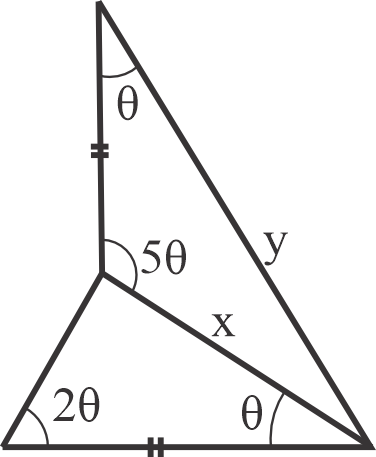
\includegraphics[width=3cm]{imagenes/general2024-I/etapa2/bio/geo1g24-II.png}
	\end{center}
	
	
	
	\begin{enumerate}[label=\alph*)]
		\item 3
		\item 1
		\item 2
		\item 4
		\item 5
	\end{enumerate}
	\textbf{Respuesta correcta:} c)
	
	\vspace{2mm}
	\textbf{Solucionario:}\\[1mm]
	
	
	
	\begin{center}
		\begin{minipage}{0.45\textwidth}
			Por congruencia de triangulos: \\
			
			De la figura se tiene:\\
			
			$2x=y$\\
			
			\fbox{$2$}$=\dfrac{y}{x}$
			
			\vspace{6mm}
		\end{minipage}
		\hfill
		\begin{minipage}{0.45\textwidth}
			\centering
			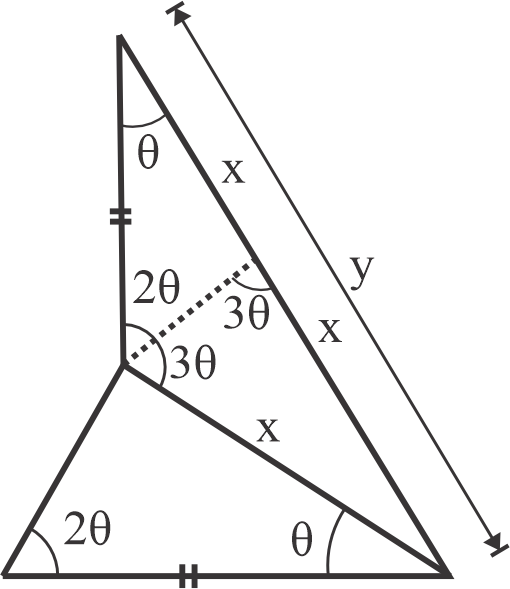
\includegraphics[width=3.5cm]{imagenes/general2024-I/etapa2/bio/geo1g24r-II.png}
		\end{minipage}
	\end{center}
	
	
	
	
	
	\vspace{6mm}
	
	\item En la figura,O es centro, UN=NA=$\sqrt{2}$ y P es Punto de Tangencia Calcule AP.
	
	\begin{center}
		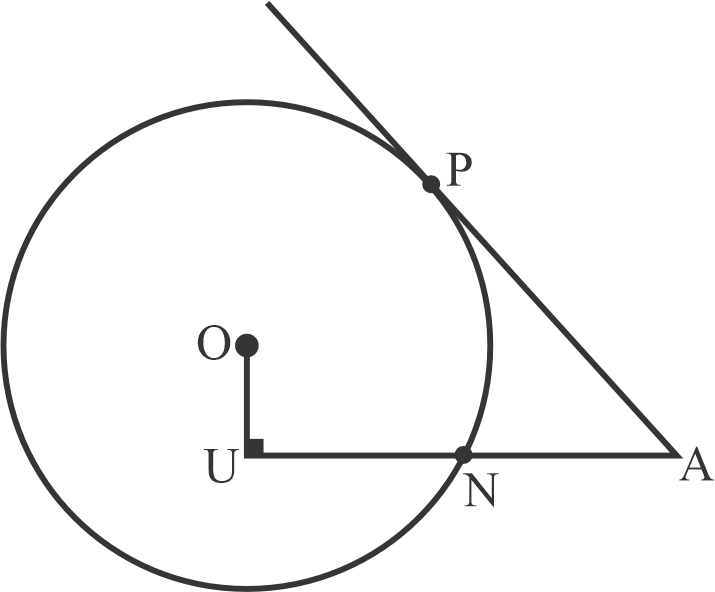
\includegraphics[width=4cm]{imagenes/general2024-I/etapa2/bio/geo2g24-II.png}
	\end{center}
	
	\begin{enumerate}[label=\alph*)]
		\item $\sqrt{3}$
		\item $\sqrt{6}$
		\item 3
		\item 6
		\item 5
	\end{enumerate}
	\textbf{Respuesta correcta:} b)
	
	\vspace{2mm}
	\textbf{Solucionario:}
	
	\begin{center}
		\begin{minipage}{0.45\textwidth}
			Por relaciones métricas \\
			
			$x^2=(3\sqrt{2})(\sqrt{2})$\\
			
			$x^2=3(2)$\\
			
			$x=$\fbox{$\sqrt{6}$}
			
			\vspace{6mm}
		\end{minipage}
		\hfill
		\begin{minipage}{0.45\textwidth}
			\centering
			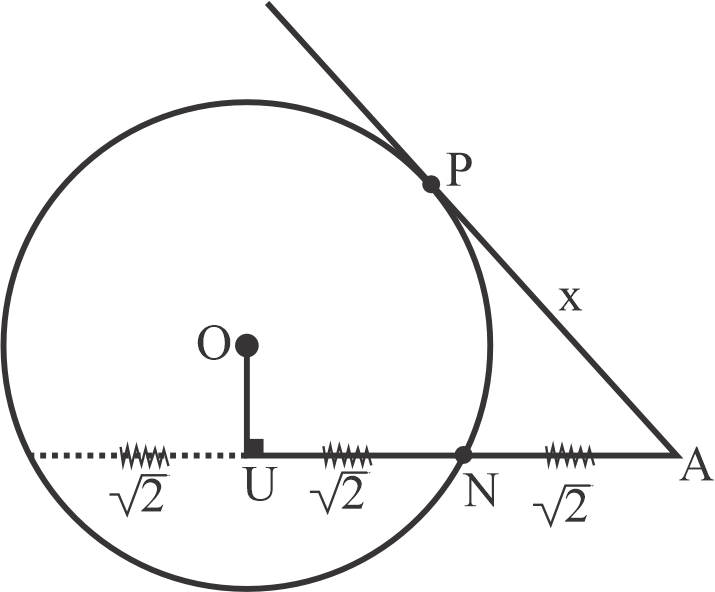
\includegraphics[width=4cm]{imagenes/general2024-I/etapa2/bio/geo2g24-IIr.png}
		\end{minipage}
	\end{center}
	
	
	\item En la figura, calcule AB.
	
	\begin{center}
		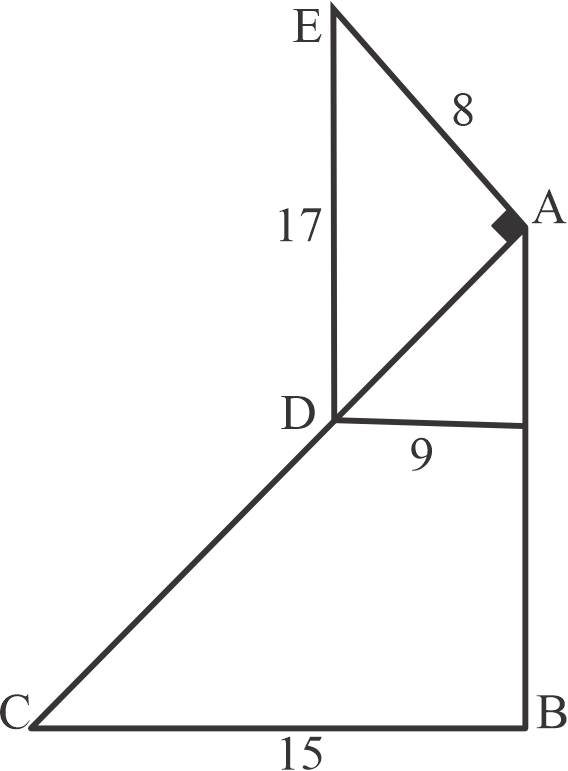
\includegraphics[width=3cm]{imagenes/general2024-I/etapa2/bio/geo3g24-II.png}
	\end{center}
	
	\begin{enumerate}[label=\alph*)]
		\item 14
		\item 15
		\item 16
		\item 18
		\item 20
	\end{enumerate}
	\textbf{Respuesta correcta:} c)
	
	\vspace{2mm}
	\textbf{Solucionario:}\\[1mm]
	
	\begin{center}
		\begin{minipage}{0.45\textwidth}
			Por semejanza de triángulos \\
			
			$\bigtriangleup APD \sim  \bigtriangleup ABC $\\
			
			$\dfrac{x}{12}=\dfrac{15}{9}$\\
			
			$x=$\fbox{$20$}
			
			\vspace{6mm}
		\end{minipage}
		\hfill
		\begin{minipage}{0.45\textwidth}
			\centering
			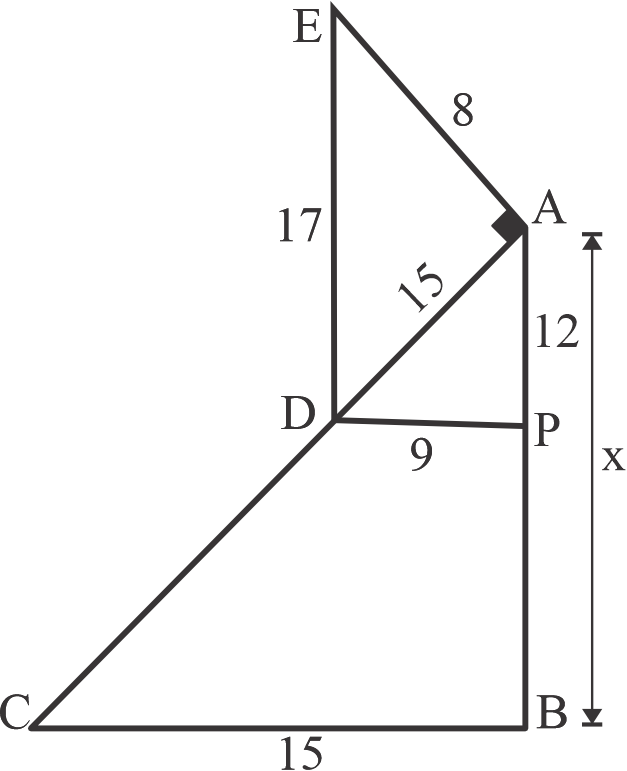
\includegraphics[width=3.8cm]{imagenes/general2024-I/etapa2/bio/geo3g24-IIr.png}
		\end{minipage}
	\end{center}
	
	\vspace{6mm}
	
	
\end{enumerate}





\subsection*{Trigonometría}

\begin{enumerate}[resume]
	
	\item En la figura, calcule ctg $\theta$
	
	\begin{center}
		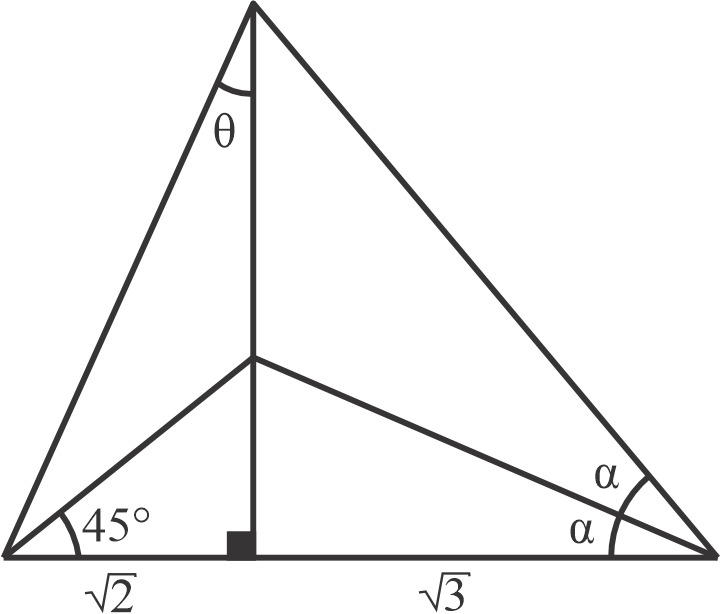
\includegraphics[width=4cm]{imagenes/general2024-I/etapa2/bio/trigo1g24-II.png}
	\end{center}
	
	\begin{enumerate}[label=\alph*)]
		\item 4
		\item $\sqrt{6}$
		\item 6
		\item 2$\sqrt{2}$
		\item 4$\sqrt{3}$
	\end{enumerate}
	\textbf{Respuesta correcta:} c)
	
	\vspace{2mm}
	\textbf{Solucionario:}
	
	$\tan \alpha = \dfrac{\sqrt{2}}{\sqrt{3}} \quad , \quad \tan 2\alpha = \dfrac{x + \sqrt{2}}{\sqrt{3}}$
	
	
	$\dfrac{2\tan \alpha}{1 - \tan^2 \alpha} = \dfrac{x + \sqrt{2}}{\sqrt{3}}$
	
	$\dfrac{\dfrac{2\sqrt{2}}{\sqrt{3}}}{1 - \dfrac{2}{3}} = \dfrac{x + \sqrt{2}}{\sqrt{3}}$
	
	$6\sqrt{2} = x + \sqrt{2}$
	
	$x = 5\sqrt{2}$
	
	$\text{ctg} \theta = \dfrac{6\sqrt{2}}{\sqrt{2}} = \fbox{6}$
	
	\vspace{6mm}
	
	\item En la figura, calcule CD
	
	\begin{center}
		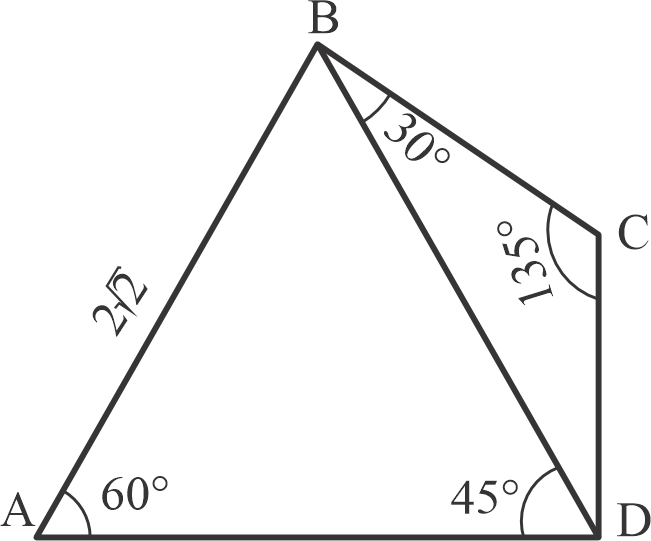
\includegraphics[width=4cm]{imagenes/general2024-I/etapa2/bio/trigo2g24-II.png}
	\end{center}
	
	\begin{enumerate}[label=\alph*)]
		\item $\sqrt{7}$
		\item $\sqrt{6}$
		\item $\sqrt{5}$
		\item $\sqrt{3}$
		\item $\sqrt{2}$
	\end{enumerate}
	\textbf{Respuesta correcta:} b)
	
	\vspace{2mm}
	\textbf{Solucionario:}
	
	\begin{center}
		\begin{minipage}{0.45\textwidth}
			
			\begin{flushright}
				ABD \qquad  | \qquad BCD\\
			\end{flushright} 
			$a = \dfrac{\text{sen}60^\circ \cdot 2\sqrt{2}}{\text{sen}45^\circ} \qquad | \qquad X = \dfrac{\text{sen}30^\circ \cdot a}{\text{sen}135^\circ}$\\
			
			De ambos\\
			
			$X = \dfrac{\text{sen}30^\circ}{\text{sen}135^\circ} \cdot \dfrac{\text{sen}60^\circ \cdot 2\sqrt{2}}{\text{sen}45^\circ}$\\
			
			\fbox{$X = \sqrt{6}$}
			
			\vspace{6mm}
		\end{minipage}
		\hfill
		\begin{minipage}{0.45\textwidth}
			\centering
			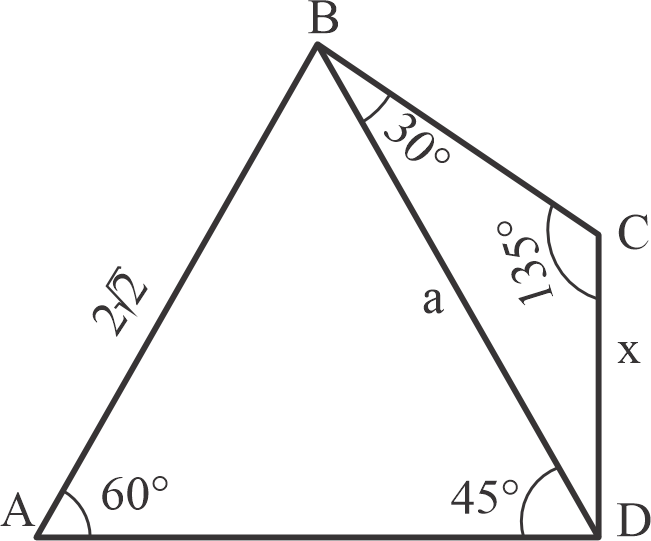
\includegraphics[width=4cm]{imagenes/general2024-I/etapa2/bio/trigo2g24-IIr.png}
		\end{minipage}
	\end{center}
	
	
	\vspace{6mm}
	
	
	\item Si $\dfrac{\csc x}{\text{sen } x} + \dfrac{\sec x}{\cos x} = n$. Calcule $\tan^2 x + \cot^2 x$
	\begin{enumerate}[label=\alph*)]
		\item $n-1$
		\item $n+2$
		\item $n-2$
		\item $n+1$
		\item $-n$
	\end{enumerate}
	\textbf{Respuesta correcta:} c)
	
	\vspace{2mm}
	\textbf{Solucionario:}\\
	
	$\dfrac{\csc x}{\text{sen } x} + \dfrac{\sec x}{\cos x} = n$
	
	$\dfrac{1}{\text{sen}^2 x} + \dfrac{1}{\cos^2 x} = n$
	
	$\dfrac{\cos^2 x + \text{sen}^2 x}{\text{sen}^2 x \cdot \cos^2 x} = n$
	
	$(\sec x \cdot \csc x)^2 = n$
	
	$(\tan x + \cot x)^2 = n$
	
	$\tan^2 x + \cot^2 x + 2 = n$
	
	$\tan^2 x + \cot^2 x = \fbox{ n - 2}$
	
	\vspace{6mm}
	
\end{enumerate}








\subsection*{Física}

\begin{enumerate}[resume]
	
	\item Ha ocurrido un accidente de tránsito y al lugar de los hechos ha llegado una ambulancia donde el personal está atendiendo a los heridos. La ambulancia estacionada tiene encendida su sirena sonora, la cual emite una potencia de $4\pi \times 10^{-2}$ W. Determine con qué nivel de intensidad percibe el sonido de la sirena una persona que se ubica a 10 m de la ambulancia.
	\begin{enumerate}[label=\alph*)]
		\item 80 dB
		\item 90 dB
		\item 70 dB
		\item 60 dB
		\item 50 dB
	\end{enumerate}
	\textbf{Respuesta correcta:} a)
	
	\vspace{2mm}
	\textbf{Solucionario:}
	
	\begin{center}
		
\includegraphics[width=5cm]{imagenes/general2024-I/etapa2/bio/fisica1g24-IIr.png}
	\end{center}
	
	$I = \dfrac{P}{A} = \dfrac{P}{4\pi r^2} = \dfrac{4\pi \cdot 10^{-2}}{4\pi \cdot (10)^2} = 10^{-4}$
	
	$\beta = 10 \log \left( \dfrac{I}{10^{-12}} \right) = 10 \log \left( \dfrac{10^{-4}}{10^{-12}} \right) = 10 \log (10^8)$
	
	$= (10)(8) = \fbox{80 \text{ dB}}$
	
	\vspace{6mm}
	
	\item Un recipiente que está térmicamente aislado contiene agua a 8 °C. Si se introduce 40 g de hielo (a 0 °C) y se observa que el hielo se funde en un 10\%. ¿cuántos gramos de agua había inicialmente en el recipiente? ($L_f = 80$ cal/g)
	\begin{enumerate}[label=\alph*)]
		\item 50 g
		\item 10 g
		\item 40 g
		\item 30 g
		\item 20 g
	\end{enumerate}
	\textbf{Respuesta correcta:} c)
	
	\vspace{2mm}
	\textbf{Solucionario:}
	
	$Q_{\text{g Hielo}} = -Q_{\text{perdido H}_2\text{O}}$
	
	$m_{\text{Hielo}} L_f = - c_{\text{H}_2\text{O}} m_{\text{H}_2\text{O}}  AT$
	
	
	$m_{\text{H}_2\text{O}} = - \dfrac{m_{\text{Hielo}} L_f}{c_{\text{H}_2\text{O}}  AT}$
	
	
	$m_{\text{H}_2\text{O}} = - \dfrac{(40)(10\%)(80)}{(1)(0-8)} = \dfrac{(4)(80)}{8}$
	
	
	$m_{\text{H}_2\text{O}} = \fbox{40 \text{ g}}$
	
	\vspace{6mm}
	
	\item Una esfera dieléctrica no conductora de radio $R$ se encuentra cargada uniformemente en todo su volumen con $+Q$. Determine la magnitud del campo eléctrico en un punto fuera de la esfera que está a una distancia $d$ del centro de la esfera.
	\begin{enumerate}[label=\alph*)]
		\item $\dfrac{1}{2\pi\varepsilon_0} \dfrac{Q}{d^2}$
		\item $\dfrac{1}{2\pi\varepsilon_0} \dfrac{Q}{R^2}$
		\item $\dfrac{1}{\pi\varepsilon_0} \dfrac{Q}{d^2}$
		\item $\dfrac{1}{4\pi\varepsilon_0} \dfrac{Q}{d^2}$
		\item $\dfrac{1}{4\pi\varepsilon_0} \dfrac{Q}{R^2}$
	\end{enumerate}
	\textbf{Respuesta correcta:} d)
	
	\vspace{2mm}
	\textbf{Solucionario:}
	
	$\phi = E A$
	
	$\phi = E A = \dfrac{Q}{\varepsilon_0}$
	
	$E = \dfrac{Q}{A \varepsilon_0}$\
	
	\fbox{$E = \dfrac{Q}{4\pi d^2 \varepsilon_0}$}
	
	\vspace{6mm}
	
\end{enumerate}





\subsection*{Química}

\begin{enumerate}[resume]
	
	\item ¿Cuál es la masa en gramos de una molécula de ácido nítrico ($\text{HNO}_3$)?\\
	($\text{H}=1$; $\text{N}=14$; $\text{O}=16$)
	\begin{enumerate}[label=\alph*)]
		\item $10,0 \times 10^{23}$
		\item $10,5 \times 10^{22}$
		\item $9,0 \times 10^{-22}$
		\item $10,5 \times 10^{-23}$
		\item $11,5 \times 10^{-23}$
	\end{enumerate}
	\textbf{Respuesta correcta:} d)
	
	\vspace{2mm}
	\textbf{Solucionario:}
	
	Determinando el peso molecular del $\text{HNO}_3$:
	
	\begin{itemize}
		\item $\text{H} = 1 \times 1 = 1$
		\item $\text{N} = 14 \times 1 = 14$
		\item $\text{O} = 16 \times 3 = 48$
	\end{itemize}
	Suma: $1 + 14 + 48 = 63\text{ g/mol}$
	
	Regla de tres simple:
	
	$63\text{ g} \text{ --- } 6,0 \times 10^{23} \text{ moléculas} $
	
	$ X \text{ ------ } 1 \text{ molécula} $
	
	$X = \dfrac{63}{6,0 \times 10^{23}} = 10,5 \times $ \fbox{$10^{-23} \text{ g}$} 
	
	\vspace{6mm}
	
	\item En un recipiente se tiene una mezcla de $1\text{ mol}$ de A y $1\text{ mol}$ de B; al reaccionar ambas sustancias se consumen $0,2\text{ moles}$ de A, estableciéndose el siguiente equilibrio a $400\text{ °C}$
	\[ \text{A}_{(g)} + \text{B}_{(g)} \rightleftharpoons 2\text{C}_{(g)} \]
	Calcule $K_c$.
	\begin{enumerate}[label=\alph*)]
		\item 0,40
		\item 0,25
		\item 0,30
		\item 0,20
		\item 0,35
	\end{enumerate}
	\textbf{Respuesta correcta:} b)
	
	\vspace{2mm}
	\textbf{Solucionario:}
	
	Sabiendo que:
	
	$\text{A}_{(g)} + \text{B}_{(g)} \rightleftharpoons 2\text{C}_{(g)}$
	
	se dan las siguientes relaciones:
	
	\begin{center}
		\begin{tabular}{lccc}
			& A & B & C \\
			Inicio & $1\text{ mol}$ & $1\text{ mol}  \rightleftharpoons $ & --- \\
			Avance & $0,2\text{ mol}$ & $0,2\text{ mol}  \rightleftharpoons$ & --- \\
			Equilibrio & $0,8\text{ mol}$ & $0,8\text{ mol} \rightleftharpoons$ & $2(0,2\text{ mol})$
		\end{tabular}
	\end{center}
	
	$ K_c = \dfrac{[\text{C}]^2}{[\text{A}][\text{B}]} \rightarrow K_c = \dfrac{(0,4)^2}{(0,8)(0,8)} \rightarrow$ \fbox{$K_c = 0,25 $}
	
	\vspace{6mm}
	
	\item Determine la masa de $\text{HNO}_3$ puro que está disuelto en $400\text{ cm}^3$ de una solución acuosa cuya densidad es $1,3\text{ g/cm}^3$ y contiene $30\%$ en masa de este ácido.
	\begin{enumerate}[label=\alph*)]
		\item 156
		\item 166
		\item 136
		\item 150
		\item 140
	\end{enumerate}
	\textbf{Respuesta correcta:} a)
	
	\vspace{2mm}
	\textbf{Solucionario:}

	Datos:
	
	$m = ?$
	
	$V = 400\text{ cm}^3$
	
	$\rho = 1,3\text{ g/cc}$
	
	Si $\rho = \dfrac{m}{V} \rightarrow m = \rho \cdot V$
	
	$ m = 1,3 \times 400 = 520\text{ g} $
	
	Si tiene el $30\%$ en masa:
	
	$ m = 520 \times 30\% $
	
	\fbox{$m = 156\text{ g} $}
	
	\vspace{6mm}
	
	\item Determine el número de fotones que emite durante 1 minuto de funcionamiento una linterna cuya potencia eléctrica es de 20 watts. Si emite una luz roja de $700\text{ nm}$ de longitud de onda.\\
	($1\text{ watt} = 1\text{ J/s}$; $h = 6,626 \times 10^{-34}\text{ J}\cdot\text{s}$; $1\text{ nm} = 10^{-9}\text{ m}$)
	\begin{enumerate}[label=\alph*)]
		\item $4,23 \times 10^{19}$
		\item $4,23 \times 10^{22}$
		\item $4,22 \times 10^{18}$
		\item $4,23 \times 10^{21}$
		\item $4,23 \times 10^{-19}$
	\end{enumerate}
	\textbf{Respuesta correcta:} d)
	
	\vspace{2mm}
	\textbf{Solucionario:}
	
	$E_{total} = \dfrac{20\text{ J}}{\text{s}} \times 60\text{ s} = 1200\text{ J}$
	
	Cálculo de la Energía de la luz roja ($\varepsilon$):
	
	$ \varepsilon = \dfrac{hc}{\lambda} = \dfrac{6,626 \times 10^{-34}\text{ J}\cdot\text{s} \times 3 \times 10^8\text{ m/s}}{700\text{ nm} \times \dfrac{1\text{ m}}{10^9\text{ nm}}} $
	
	$ \varepsilon = 2,84 \times 10^{-19}\text{ J} $
	
	Número de fotones ($N_{fot}$):

	$ N_{fot} = \dfrac{E_{total}}{\varepsilon} = \dfrac{1200\text{ J}}{2,84 \times 10^{-19}\text{ J}} $\\
	
	\fbox{$ N_{fot} = 4,23 \times 10^{21} $}
	
	\vspace{6mm}
	
	\item Halle el volumen de aire que se necesita para la combustión de 3 litros de acetileno ($\text{C}_2\text{H}_2$) y el volumen de dióxido de carbono ($\text{CO}_2$), según la reacción:
	\[ \text{C}_2\text{H}_2 + \text{O}_2 \rightarrow \text{CO}_2 + \text{H}_2\text{O} \]
	(Aire: $\text{O}_2 = 20\%$; $\text{N}_2 = 80\%$ en volumen)
	\begin{enumerate}[label=\alph*)]
		\item $35,7\text{ L}$ y $6\text{ L}$
		\item $3,7\text{ L}$ y $5\text{ L}$
		\item $37,5\text{ L}$ y $3\text{ L}$
		\item $7,5\text{ L}$ y $6\text{ L}$
		\item $37,5\text{ L}$ y $6\text{ L}$
	\end{enumerate}
	\textbf{Respuesta correcta:} e)
	
	\vspace{2mm}
	\textbf{Solucionario:}\\[1mm]
	Se tiene la reacción y la balanceamos:
	
	$ 1\text{C}_2\text{H}_2 + \dfrac{5}{2}\text{O}_2 \rightarrow 2\text{CO}_2 + \text{H}_2\text{O} $\\
	
	Relación de volúmenes:
	
	$ 1\text{V}_{\text{C}_2\text{H}_2} \text{ --- } \dfrac{5}{2}\text{V}_{\text{O}_2} \text{ --- } 2\text{V}_{\text{CO}_2} $
	
	$ 3\text{ L} \text{ --------- } \text{V}_{\text{O}_2} \text{ ------ } \text{V}_{\text{CO}_2} $
	
	Cálculo de $\text{V}_{\text{O}_2}$:
	
	$ \text{V}_{\text{O}_2} = \dfrac{(3\text{ L})(\dfrac{5}{2}\text{ V})}{1\text{ V}} = 7,5\text{ L} $
	Cálculo de $\text{V}_{\text{CO}_2}$:
	
	$ \text{V}_{\text{CO}_2} = \dfrac{(3\text{ L})(2\text{ V})}{1\text{ V}} = 6\text{ L} $
	Cálculo del volumen de aire:
	
	$ V_{aire} = \dfrac{\text{V}_{\text{O}_2}}{20\%} \rightarrow V_{aire} = \dfrac{7,5\text{ L}}{20\%} \rightarrow$  \fbox{$V_{aire} = 37,5\text{ L} $}
	
	\vspace{6mm}
	
\end{enumerate}






\subsection*{Biología y Anatomía}

\begin{enumerate}[resume]
	
	\item Es la cantidad de aire que permanece en los pulmones al final de una espiración normal. Su valor resulta de la suma del volumen residual más el volumen de reserva espiratorio.
	\begin{enumerate}[label=\alph*)]
		\item volumen de aire corriente (VAC)
		\item volumen de reserva inspiratoria (VRI)
		\item volumen de respiración minuto (Vm)
		\item capacidad funcional inspiratoria (CFI)
		\item capacidad funcional residual (CFR)
	\end{enumerate}
	\textbf{Respuesta correcta:} e)
	
	\vspace{2mm}
	\textbf{Solucionario:}\\[1mm]
	La Capacidad Funcional Residual (CFR) es la suma del Volumen de Reserva Espiratorio (VRE) y el Volumen Residual (VR). Representa el aire que queda en los pulmones tras una espiración pasiva.
	
	\vspace{6mm}
	
	\item ¿Cuál es el microorganismo de importancia en la industria panificadora e industria de bebidas alcohólicas?
	\begin{enumerate}[label=\alph*)]
		\item Escherichia coli
		\item Rhizobium leguminosarum
		\item Saccharomyces cerevisiae
		\item Clostridium acetobutylicum
		\item Bacillus thuringiensis
	\end{enumerate}
	\textbf{Respuesta correcta:} c)
	
	\vspace{2mm}
	\textbf{Solucionario:}\\[1mm]
	\textit{Saccharomyces cerevisiae} es una levadura unicelular fundamental en la fermentación alcohólica, proceso clave para la producción de pan, cerveza y vino.
	
	\vspace{6mm}
	
	\item Son dos masas ovoideas formadas por sustancia gris, localizadas a ambos lados del tercer ventrículo. Su función es la de servir de estación de relevo para todos los impulsos sensitivos.
	\begin{enumerate}[label=\alph*)]
		\item Aracnoides
		\item Tálamo
		\item Duramadre
		\item Hipotálamo
		\item Cerebelo
	\end{enumerate}
	\textbf{Respuesta correcta:} b)
	
	\vspace{2mm}
	\textbf{Solucionario:}\\[1mm]
	El tálamo actúa como el principal centro de relevo sensorial de la zona cerebral; procesa y transmite la información sensorial a las áreas correspondientes de la corteza cerebral (excepto el olfato).
	
	\vspace{6mm}
	
	\item Los genotipos $X^dY$ y RHrh corresponde a:
	\begin{enumerate}[label=\alph*)]
		\item varón portador, Rh (+)
		\item varón hemofílico, Rh (-)
		\item varón daltónico, Rh (+)
		\item varón daltónico, Rh (-)
		\item varón sano, Rh (+)
	\end{enumerate}
	\textbf{Respuesta correcta:} c)
	
	\vspace{2mm}
	\textbf{Solucionario:}\\[1mm]
	El genotipo $X^dY$ indica un varón que posee el gen recesivo del daltonismo en su único cromosoma X, por lo tanto es daltónico. El genotipo $RHrh$ es heterocigoto, lo que se manifiesta como fenotipo Rh positivo.
	
	\vspace{6mm}
	
	\item El hígado, considerado como "laboratorio central" del cuerpo, puede realizar más de cien funciones diferentes. Respecto a su participación en el proceso de la digestión, señale la secuencia correcta de verdadero (V) y falso (F).
	\begin{itemize}
		\item[I.] Los conductos hepático común y acino portal forman el colédoco.
		\item[II.] La función del hígado en la digestión es producir la bilis.
		\item[III.] Las sales biliares se sintetizan a partir de los fosfolípidos y aminoácidos.
		\item[IV.] La bilis es almacenada y concentrada en la vesícula biliar.
		\item[V.] La bilis emulsifica la grasa formando micelas para su absorción.
	\end{itemize}
	\begin{enumerate}[label=\alph*)]
		\item FFFVV
		\item VFFVF
		\item FVFVV
		\item VVFFF
		\item FVVFV
	\end{enumerate}
	\textbf{Respuesta correcta:} c)
	
	\vspace{2mm}
	\textbf{Solucionario:}\\[1mm]
	I(F): El colédoco se forma por la unión del conducto cístico y el hepático común.\\
	II(V): El hígado produce bilis. \\
	III(F): Se sintetizan a partir del colesterol. \\
	IV(V): La vesícula almacena la bilis. \\
	V(V): La emulsificación facilita la digestión de grasas.
	
	\vspace{6mm}
	
	\item La oxitocina es producida en el \underline{\hspace{3cm}} y almacenada en la \underline{\hspace{3cm}}.
	\begin{enumerate}[label=\alph*)]
		\item núcleo paraventricular - neurohipófisis
		\item sistema portal hipofisiario - adenohipófisis
		\item lóbulo anterior - neurohipófisis
		\item lóbulo posterior - quiasma óptica
		\item núcleo supraóptico - neurofisina
	\end{enumerate}
	\textbf{Respuesta correcta:} a)
	
	\vspace{2mm}
	\textbf{Solucionario:}\\[1mm]
	La oxitocina se sintetiza principalmente en el núcleo paraventricular del hipotálamo y se transporta para su almacenamiento y posterior liberación a la neurohipófisis (hipófisis posterior).
	
	\vspace{6mm}
	
	
	
	
	
\end{enumerate}



\subsection*{Psicología y Filosofía}

\begin{enumerate}[resume]
	
	\item Cada vez que el profesor de inglés menciona la palabra examen, Ramiro experimenta una baja en su temperatura y comienza a tiritar ante la palabra examen. La conducta de tiritar ante la palabra examen se denomina:
	\begin{enumerate}[label=\alph*)]
		\item condicionada.
		\item incondicionada.
		\item refleja.
		\item orientadora.
		\item neutral.
	\end{enumerate}
	\textbf{Respuesta correcta:} a)
	
	\vspace{2mm}
	\textbf{Solucionario:}\\[1mm]
	En el condicionamiento clásico, una respuesta que originalmente era natural (incondicionada) ante un estímulo biológico, pasa a ser una respuesta condicionada cuando es provocada por un estímulo previamente neutro (la palabra "examen") que ha sido asociado al evento original.
	
	\vspace{6mm}
	
	\item Un taxista dice que las mujeres deberían estar cocinando y no conduciendo. Esta manera de pensar se denomina:
	\begin{enumerate}[label=\alph*)]
		\item discriminación.
		\item actitud.
		\item prejuicio.
		\item aprendizaje.
		\item estereotipo.
	\end{enumerate}
	\textbf{Respuesta correcta:} c)
	
	\vspace{2mm}
	\textbf{Solucionario:}\\[1mm]
	El prejuicio es una actitud preconcebida, generalmente negativa, hacia los miembros de un grupo social. En este caso, el juicio de valor sobre lo que "deberían" hacer las mujeres refleja una predisposición afectiva y cognitiva antes de conocer la capacidad individual de la persona.
	
	\vspace{6mm}
	
	\item Para los estoicos, ¿Cuándo uno es feliz?
	\begin{enumerate}[label=\alph*)]
		\item Cuando se practica la prudencia.
		\item Cuando se logra la autarquía.
		\item Cuando se acepta lo que se es.
		\item Cuando se logra tener placer.
		\item Cuando se hace lo que conviene a la mayoría.
	\end{enumerate}
	\textbf{Respuesta correcta:} c)
	
	\vspace{2mm}
	\textbf{Solucionario:}\\[1mm]
	La ética estoica propone que la felicidad se alcanza a través de la "apatheia" y la aceptación del orden racional del universo. Aceptar lo que uno es y lo que le acontece (el destino) permite vivir en armonía con la naturaleza y alcanzar la tranquilidad del alma.
	
	\vspace{6mm}
	
	\item Los nativos de África tienen una forma de valorar la belleza que difiere de los nativos de las tribus sudamericanas, esto sería una idea que apoyaría la teoría de:
	\begin{enumerate}[label=\alph*)]
		\item Sócrates
		\item Protágoras
		\item Demócrito
		\item Anaxágoras
		\item Heráclito
	\end{enumerate}
	\textbf{Respuesta correcta:} b)
	
	\vspace{2mm}
	\textbf{Solucionario:}\\[1mm]
	Protágoras, con su máxima "el hombre es la medida de todas las cosas", sostiene el relativismo. Esto implica que valores como la belleza no son universales, sino que dependen de la percepción de cada individuo o cultura.
	
	\vspace{6mm}
	
\end{enumerate}


\subsection*{Geografía}

\begin{enumerate}[resume]
	
	\item La consecuencia del movimiento de rotación de la Tierra es la sucesión del día y la noche. Entonces, por regla general, ...
	\begin{enumerate}[label=\alph*)]
		\item en todo lugar que se localiza al oeste de otro amanece primero
		\item en todo lugar que se localiza al este de otro amanece primero
		\item en todo lugar que se localiza al norte de otro amanece primero
		\item en todo lugar que se localiza al sur de otro amanece primero
		\item en todo lugar que se localiza delante de otro amanece primero
	\end{enumerate}
	\textbf{Respuesta correcta:} b)
	
	\vspace{2mm}
	\textbf{Solucionario:}\\[1mm]
	Debido a que la Tierra rota de oeste a este, los lugares situados más hacia el oriente (este) visualizan el sol antes que los lugares al occidente. Por lo tanto, el amanecer ocurre primero en las zonas orientales.
	
	\vspace{6mm}
	
	\item La biodiversidad es la variabilidad de los organismos vivos por:
	\begin{enumerate}[label=\alph*)]
		\item ecosistemas.
		\item especies.
		\item recursos naturales.
		\item unidad de superficie.
		\item afinidad biológica.
	\end{enumerate}
	\textbf{Respuesta correcta:} d)
	
	\vspace{2mm}
	\textbf{Solucionario:}\\[1mm]
	En ciertos contextos de análisis geográfico y ecológico, la biodiversidad se cuantifica y evalúa como la variabilidad o riqueza de especies y ecosistemas presentes en una unidad de superficie determinada, permitiendo comparar la densidad biológica entre distintas regiones.
	
	\vspace{6mm}
	
\end{enumerate}


\subsection*{Historia}

\begin{enumerate}[resume]
	
	\item Las investigaciones de Louis Pasteur (1822 - 1895) sobre la fermentación permitió el desarrollo de la:
	\begin{enumerate}[label=\alph*)]
		\item fitología.
		\item microbiología.
		\item virología.
		\item ficología.
		\item micología.
	\end{enumerate}
	\textbf{Respuesta correcta:} b)
	
	\vspace{2mm}
	\textbf{Solucionario:}\\[1mm]
	Louis Pasteur demostró que los procesos de fermentación y enfermedades infecciosas son causados por microorganismos, lo que dio inicio a la microbiología como ciencia médica y biológica.
	
	\vspace{6mm}
	
	\item El Hospital Naval, el Hospital Militar y el Hospital Central del Empleado en Lima, así como los hospitales regionales en los departamentos, fueron construidos durante el gobierno del Presidente:
	\begin{enumerate}[label=\alph*)]
		\item Manuel A. Odría.
		\item Manuel Prado Ugarteche.
		\item José Luis Bustamante y Rivero.
		\item Ricardo Pérez Godoy.
		\item Augusto B. Leguía.
	\end{enumerate}
	\textbf{Respuesta correcta:} a)
	
	\vspace{2mm}
	\textbf{Solucionario:}\\[1mm]
	El gobierno de Manuel A. Odría (1948-1956) se caracterizó por una fuerte inversión en salud y educación, construyendo las Grandes Unidades Escolares y los principales centros hospitalarios de la capital y provincias.
	
	\vspace{6mm}
	
\end{enumerate}

\subsection*{Educación Cívica}

\begin{enumerate}[resume]
	
	\item La \underline{\hspace{3cm}} es un organismo cuyo propósito es mejorar a través de la acción internacional las condiciones de trabajo y los niveles de vida, promoviendo la estabilidad social y económica.
	\begin{enumerate}[label=\alph*)]
		\item OMS
		\item OMC
		\item OIT
		\item UNESCO
		\item UNICEF
	\end{enumerate}
	\textbf{Respuesta correcta:} c)
	
	\vspace{2mm}
	\textbf{Solucionario:}\\[1mm]
	La Organización Internacional del Trabajo (OIT) es el organismo especializado de la ONU que se ocupa de los asuntos relativos al trabajo y las relaciones laborales a nivel mundial.
	
	\vspace{6mm}
	
	\item Una de las atribuciones del Congreso de la República del Perú, de acuerdo a la Constitución, es:
	\begin{enumerate}[label=\alph*)]
		\item conceder indultos y conmutar penas.
		\item convocar a elecciones generales, parlamentarias, regionales y locales.
		\item aprobar el presupuesto y la Cuenta General de la República.
		\item velar por el orden interno y externo.
		\item dirigir la política general del Gobierno.
	\end{enumerate}
	\textbf{Respuesta correcta:} c)
	
	\vspace{2mm}
	\textbf{Solucionario:}\\[1mm]
	Dentro de la función legislativa y de control, el Congreso tiene la facultad exclusiva de aprobar el presupuesto público propuesto por el Ejecutivo y revisar la ejecución del mismo a través de la Cuenta General.
	
	\vspace{6mm}
	
\end{enumerate}


\subsection*{Economía}

\begin{enumerate}[resume]
	
	\item La palta, conocida también como "oro verde", ocupó en los últimos años los primeros lugares en exportación del grupo de los productos agroindustriales. Según el BCRP, el producto señalado es considerado de exportación:
	\begin{enumerate}[label=\alph*)]
		\item no tradicional.
		\item temporal.
		\item tradicional.
		\item definitiva.
		\item sin valor comercial.
	\end{enumerate}
	\textbf{Respuesta correcta:} a)
	
	\vspace{2mm}
	\textbf{Solucionario:}\\[1mm]
	Las exportaciones no tradicionales son productos que tienen un mayor valor agregado o que históricamente no eran el fuerte de la balanza comercial. La palta pertenece al sector agroindustrial, el cual es un eje clave de las exportaciones no tradicionales en el Perú.
	
	\vspace{6mm}
	
	\item El incremento del precio de los insumos para la elaboración de un bien en un mercado de competencia perfecta genera:
	\begin{enumerate}[label=\alph*)]
		\item un aumento de la demanda.
		\item un aumento de las ganancias del vendedor.
		\item un incremento de la cantidad ofertada.
		\item una expansión de la oferta.
		\item una contracción de la oferta.
	\end{enumerate}
	\textbf{Respuesta correcta:} e)
	
	\vspace{2mm}
	\textbf{Solucionario:}\\[1mm]
	Cuando los costos de producción aumentan (debido al alza de precio de los insumos), producir el mismo bien resulta más caro. Esto provoca que los productores estén dispuestos a ofrecer menos cantidad al mismo precio, lo que se traduce gráficamente como un desplazamiento de la curva de oferta hacia la izquierda (contracción).
	
	\vspace{6mm}
	
\end{enumerate}

\subsection*{Comunicación}

\begin{enumerate}[resume]
	
	\item La tuberculosis es una enfermedad pulmonar contagiosa que se transmite por el aire. \\ ¿A qué tipo de texto corresponde?
	\begin{enumerate}[label=\alph*)]
		\item Narrativo
		\item Expositivo
		\item Instructivo
		\item Argumentativo
		\item Descriptivo
	\end{enumerate}
	\textbf{Respuesta correcta:} b)
	
	\vspace{2mm}
	\textbf{Solucionario:}\\[1mm]
	El texto presenta información objetiva y conceptos sobre una realidad específica (la tuberculosis) con el fin de informar al receptor, característica principal de los textos expositivos.
	
	\vspace{6mm}
	
	\item Consiste en expresar de manera condensada y coherente el contexto esencial del texto. Se realiza a partir de la síntesis global del contenido. \\ ¿A qué tipo de técnica de estudio corresponde?
	\begin{enumerate}[label=\alph*)]
		\item Subrayado
		\item Esquema
		\item Notas al margen
		\item Secuencia
		\item Resumen
	\end{enumerate}
	\textbf{Respuesta correcta:} e)
	
	\vspace{2mm}
	\textbf{Solucionario:}\\[1mm]
	El resumen es la técnica de estudio que reduce un texto a sus ideas fundamentales, manteniendo la coherencia y la esencia del mensaje original pero de forma abreviada.
	
	\vspace{6mm}
	
	\item Es una forma de interacción comunicativa oral y planificada, en la que distintos interlocutores asumen posturas contrarias a partir de un tema polémico.
	\begin{enumerate}[label=\alph*)]
		\item Seminario
		\item Debate
		\item Informe oral
		\item Entrevista
		\item Plenario
	\end{enumerate}
	\textbf{Respuesta correcta:} b)
	
	\vspace{2mm}
	\textbf{Solucionario:}\\[1mm]
	El debate es una técnica de comunicación que consiste en la confrontación de ideas u opiniones diferentes sobre un tema determinado, donde los participantes defienden sus posturas con argumentos.
	
	\vspace{6mm}
	
	\item El \underline{\hspace{3cm}} es un organizador gráfico que resume un texto de manera organizada, jerarquizada y conectada, a través de líneas y palabras de enlace.
	\begin{enumerate}[label=\alph*)]
		\item diagrama de Ishikawa
		\item mapa mental
		\item mapa conceptual
		\item mapa semántico
		\item cuadro sinóptico
	\end{enumerate}
	\textbf{Respuesta correcta:} c)
	
	\vspace{2mm}
	\textbf{Solucionario:}\\[1mm]
	El mapa conceptual se caracteriza específicamente por el uso de conceptos encerrados en elipses o cuadros (nodos) que se relacionan entre sí mediante líneas y palabras de enlace, siguiendo una estructura jerárquica.
	
	\vspace{6mm}
	
\end{enumerate}


\subsection*{Literatura}

\begin{enumerate}[resume]
	
	\item Los poetas populares del incanato se denominaban:
	\begin{enumerate}[label=\alph*)]
		\item amautas.
		\item haravicus.
		\item purej.
		\item quipucamayoc.
		\item tucuy-ricuy.
	\end{enumerate}
	\textbf{Respuesta correcta:} b)
	
	\vspace{2mm}
	\textbf{Solucionario:}\\[1mm]
	En el Imperio Incaico, los haravicus eran los poetas populares que expresaban los sentimientos de la comunidad (amor, agro, guerra) a través de la lírica, a diferencia de los amautas, que eran los maestros y encargados de la educación formal de la nobleza.
	
	\vspace{6mm}
	
	\item "Soy cantor de América, autóctono y salvaje mi lira tiene un alma, mi canto un ideal. Mi verso no se mece colgado de un ramaje con un vaivén pausado de hamaca tropical" \\ \\ Estos versos pertenecen a:
	\begin{enumerate}[label=\alph*)]
		\item Dante Nava.
		\item Abraham Valdelomar.
		\item Ciro Alegría.
		\item José Santos Chocano.
		\item Arturo Peralta.
	\end{enumerate}
	\textbf{Respuesta correcta:} d)
	
	\vspace{2mm}
	\textbf{Solucionario:}\\[1mm]
	Estos versos corresponden al poema "Blasón", perteneciente al libro \textit{Alma América} de José Santos Chocano. Es el máximo representante del Modernismo en el Perú y se autodenominó "El Cantor de América".
	
	\vspace{6mm}
	
\end{enumerate}



\subsection*{Razonamiento Matemático}

\begin{enumerate}[resume]
	
	\item De cuántas formas se puede leer la palabra UNAP?
	
	\begin{center}
		\begin{tabular}{cccc}
			U & N & A & P \\
			N & A & P & A \\
			A & P & A & N \\
			P & A & N & U \\
		\end{tabular}
	\end{center}
	\begin{enumerate}[label=\alph*)]
		\item 32
		\item 16
		\item 20
		\item 18
		\item 24
	\end{enumerate}
	\textbf{Respuesta correcta:} b)
	
	\vspace{2mm}
	\textbf{Solucionario:}
	
	Identificamos la forma triangular que se presenta en el arreglo.
	
	
	\begin{center}
		\begin{tikzpicture}[scale=0.7, every node/.style={font=\sffamily\bfseries}]
			% Matriz de letras (Arreglo de la palabra UNAP)
			\node (u1) at (0,3) {U}; \node at (1,3) {N}; \node at (2,3) {A}; \node (p1) at (3,3) {P};
			\node at (0,2) {N}; \node at (1,2) {A}; \node (p2) at (2,2) {P}; \node at (3,2) {A};
			\node at (0,1) {A}; \node (p3) at (1,1) {P}; \node at (2,1) {A}; \node at (3,1) {N};
			\node (p4) at (0,0) {P}; \node at (1,0) {A}; \node at (2,0) {N}; \node (u2) at (3,0) {U};
			
			% CUADRO ROJO (Triángulo superior izquierdo)
			% Alineado para envolver desde U (0,3) hasta la diagonal de Ps
			\draw[red, thick, rounded corners=8pt] 
			(-0.4, 3.4) -- (3.6, 3.4) -- (-0.4, -0.6) -- cycle;
			
			% CUADRO AZUL (Triángulo inferior derecho)
			% Alineado para envolver desde U (3,0) hasta la diagonal de Ps
			\draw[blue, thick, rounded corners=8pt] 
			(3.4, -0.4) -- (-0.6, -0.4) -- (3.4, 3.6) -- cycle;
			
		\end{tikzpicture}
	\end{center}
	
	\begin{itemize}
		\item UNAP 4 Letras
		\item $2^{n-1} = 2^{4-1} = 2^{3} = 8$
		\item 8 Formas
	\end{itemize}
	
	Se observa 2 veces la forma triangular
	
	$8 + 8 =$\fbox{$ 16$} Formas
	
	\vspace{6mm}
	
	
	
	
	
	
	
	
	
	\item Halle el área de la región sombreada si el lado del cuadrado $ABCD$ es $4u$.
	
	\begin{center}
		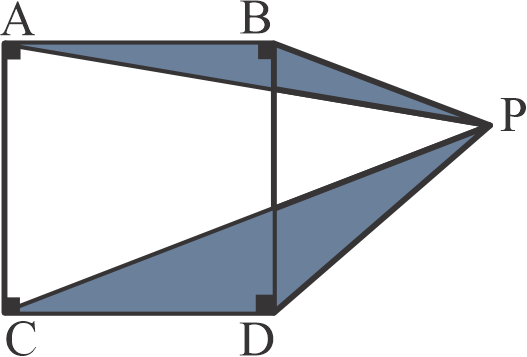
\includegraphics[width=4.4cm]{imagenes/general2024-I/etapa2/bio/rm2g24-II.png}
	\end{center}
	
	\begin{enumerate}[label=\alph*)]
		\item $5u^2$
		\item $16u^2$
		\item $12u^2$
		\item $8^2$
		\item $4u^2$
	\end{enumerate}
	\textbf{Respuesta correcta:}d)
	
	\vspace{2mm}
	\textbf{Solucionario:}
	
	\begin{center}
		\begin{minipage}{0.45\textwidth}
			
			$H1 + H2 = 4$\\
			
			$A_s = A_{s1} + A_{s2} = \dfrac{4 \cdot H1}{2} + \dfrac{4 \cdot H2}{2}$ \\
			
			$A_s = 2 H1 + 2 H2$ \\
			
			$A_s = 2 (H1 + H2)$ \\
			
			$A_s = 2 (4)$ \\
			
			\fbox{$A_s = 8$}
			
			\vspace{6mm}
		\end{minipage}
		\hfill
		\begin{minipage}{0.45\textwidth}
			\centering
			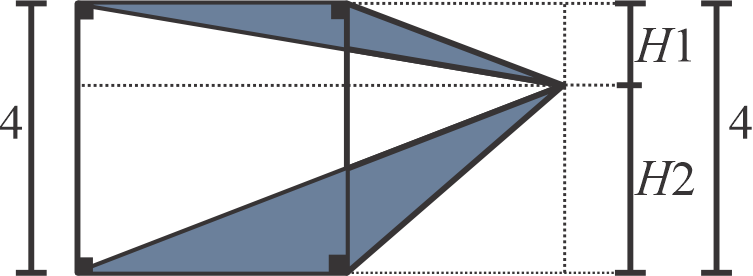
\includegraphics[width=5.4cm]{imagenes/general2024-I/etapa2/bio/rm2g24-IIr.png}
		\end{minipage}
	\end{center}
	
	
	
	
	\item Pablito le dice a José: "La suma de nuestras edades es 46 años y tu edad es el triple de la edad que tenías cuando yo tenía el triple de la edad que tuviste cuando yo nací". ¿Qué edad tiene José?
	
	\begin{enumerate}[label=\alph*)]
		\item 28
		\item 40
		\item 18
		\item 8
		\item 24
	\end{enumerate}
	\textbf{Respuesta correcta:} e)
	
	\vspace{2mm}
	\textbf{Solucionario:}
	
	
	
	\begin{center}
		
		\begin{tikzpicture}[x=1.5cm, y=0.8cm, every node/.style={font=\footnotesize\sffamily}]
			% Líneas del cuadro
			\draw (0,0) rectangle (4,3);
			\draw (0,1) -- (4,1);
			\draw (0,2) -- (4,2);
			\draw (1.2,0) -- (1.2,3);
			\draw (2.1,0) -- (2.1,2);
			\draw (3,0) -- (3,2);
			
			% Encabezados
			
			\node at (1.65,2.5) {Tuviste};
			\node at (2.55,2.5) {Tenías};
			\node at (3.5,2.5) {Tienes};
			
			% Filas
			\node at (0.6,1.5) {Pablito};
			\node at (1.65,1.5) {0};
			\node at (2.55,1.5) {$y$};
			\node at (3.5,1.5) {$3y+2x$};
			
			\node at (0.6,0.5) {José};
			\node at (1.65,0.5) {$x$};
			\node at (2.55,0.5) {$3x$};
			\node at (3.5,0.5) {$3x$};
			\node at (3.5,-0.6) {$46$ suma};
			% Flechas de suma en aspa (opcionales según imagen)
			\draw[red, <->] (1.8,1.3) -- (2.4,0.7);
			\draw[red, <->] (1.8,0.7) -- (2.4,1.3);
			\draw[red, <->] (2.7,1.3) -- (3.3,0.7);
			\draw[red, <->] (2.7,0.7) -- (3.3,1.3);
		\end{tikzpicture}
		
		
		
		
	\end{center}
	
	
	
	
	Aplicamos la suma en aspa:
	
	$0 + 3x = y + 3y \Rightarrow x = 4y$ .....(I) 
	
	Planteando la primera afirmación:
	
	$(3y + 2x) + 3x = 46$ .....(II)
	
	$3y + 5x = 46$ 
	
	(I) en (II): 
	
	$3y + 5(4y) = 46 \Rightarrow y = 2 \Rightarrow x = 8$ 
	
	$\therefore$ José tiene $3(8) = 24$ años.
	
	\vspace{4mm}
	\fbox{José tiene 24 años}
	
	
	
	
	
	
	\item Se tiene un número impar, se le añade el par de números impares que le anteceden y los tres números pares que son inmediatamente anteriores a dicho número, dando un resultado de 939 unidades. Halle la suma de cifras del número impar mencionado.
	
	\begin{enumerate}[label=\alph*)]
		\item 15
		\item 16
		\item 13
		\item 19
		\item 26
	\end{enumerate}
	\textbf{Respuesta correcta: a)}
	
	\vspace{2mm}
	\textbf{Solucionario:}
	
	Suma de cifras del número impar mencionado:
	
	$\qquad\underbrace{2x+1}_{} \quad \quad +\qquad \underbrace{(2x-1), (2x-3)}_{} +\quad \underbrace{2x, 2x-2, 2x-4}_{} = 939$
	
	$\Rightarrow \left( \text{número impar} \right) + \left( \begin{tabular}{c} 2 números \\ impares que \\ anteceden \end{tabular} \right) + \left( \begin{tabular}{c} 3 números \\ pares que \\ anteceden \end{tabular} \right) = 939$
	
	
	\vspace{2mm}
	Sumando:
	
	$12x - 9 = 939$ 
	
	$x = 79$
	
	
	Número impar $= 2x + 1 = 2(79) + 1 = 159$
	
	Suma de cifras: $1 + 5 + 9 = $\fbox{15}
	
	
	\item ¿Cuántas diagonales hay en la figura?
	
	\begin{center}
		
\includegraphics[width=3cm]{imagenes/general2024-I/etapa2/bio/rm5g24-II.png}
	\end{center}
	
	
	\begin{enumerate}[label=\alph*)]
		\item 24
		\item 20
		\item 22
		\item 24
		\item 26
	\end{enumerate}
	\textbf{Respuesta correcta:} c)
	
	\vspace{2mm}
	\textbf{Solucionario:}
	
	Como cada cuadrilátero tiene dos diagonales, entonces, el número de diagonales será el doble del número de cuadriláteros:
	
	
	
	
	\begin{center}
		\begin{minipage}{0.45\textwidth}
			
			\begin{itemize}
				\item 3 cuadriláteros ($a, d, e$)
				\item 5 cuadriláteros 
				
				($ad, de, ec, bc, ab$)
				\item 2 cuadriláteros ($abc, bce$)
				\item 1 cuadrilátero ($abcde$)
			\end{itemize}
			Total: 11 cuadriláteros.\\
			
			\fbox{$\therefore$ Hay 22 diagonales.}
			
			
			\vspace{6mm}
		\end{minipage}
		\hfill
		\begin{minipage}{0.45\textwidth}
			\centering
			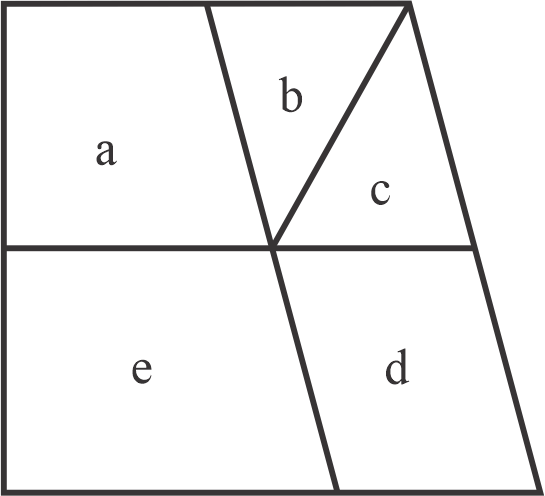
\includegraphics[width=3cm]{imagenes/general2024-I/etapa2/bio/rm5g24-IIr.png}
		\end{minipage}
	\end{center}
	
	\vspace{6mm}
	
	
	
	\item Un total de 45 estrechadas de mano se efectuaron al final de una reunión, suponiendo que cada uno de los participantes es cortés con cada uno de los demás. Determine el número de personas participantes de la reunión.
	\begin{enumerate}[label=\alph*)]
		\item 8
		\item 9
		\item 11
		\item 10
		\item 12
	\end{enumerate}
	\textbf{Respuesta correcta:} d)
	
	\vspace{2mm}
	\textbf{Solucionario:}
	
	$n$: número de personas participantes. El saludo es de dos en dos (combinatoria).
	
	$ C_{2}^{n} = \dfrac{n!}{(n-2)! 2!} = \dfrac{n(n-1)(n-2)!}{2 \times 1 \times (n-2)!} = \dfrac{n(n-1)}{2} $
	
	$ 45 = \dfrac{n(n-1)}{2} $
	
	$ 90 = n(n-1) = 10(9) $
	
	$\therefore  \fbox{n = 10}$
	
	\vspace{6mm}
	
	
	
\end{enumerate}









\subsection*{Razonamiento Verbal}

\begin{enumerate}[resume]
	
	\item Identifique el par analógico\\
	INSPIRACIÓN : PULMONES ::
	\begin{enumerate}[label=\alph*)]
		\item circulación : corazón.
		\item ingestión : estómago.
		\item segregación : páncreas.
		\item asimilación : cerebro.
		\item inoculación : vacuna.
	\end{enumerate}
	\textbf{Respuesta correcta:} b)
	
	\vspace{2mm}
	\textbf{Solucionario:}\\[1mm]
	La relación es de función-órgano: la inspiración es el proceso principal de ingreso que se realiza en los pulmones, así como la ingestión es el proceso de ingreso de alimento que se realiza en el estómago.
	
	\vspace{6mm}
	
	\item Su exposición solo fue una narrativa sin evidencia empírica. El sinónimo de la palabra NARRATIVA es:
	\begin{enumerate}[label=\alph*)]
		\item sustento.
		\item razón.
		\item prosa.
		\item motivo.
		\item pilar.
	\end{enumerate}
	\textbf{Respuesta correcta:} c)
	
	\vspace{2mm}
	\textbf{Solucionario:}\\[1mm]
	En el contexto literario y lingüístico, la narrativa está asociada formalmente a la prosa (forma de expresión habitual no sujeta a medida), a diferencia de otros términos que implican fundamentación lógica.
	
	\vspace{6mm}
	
	\item Complete la Oración\\
	La \underline{\hspace{2cm}} puede ser definida como una capa delgada de tejido animal que envuelve algún órgano o separa dos \underline{\hspace{2cm}}.
	\begin{enumerate}[label=\alph*)]
		\item piel - cuerpos
		\item célula - zonas
		\item histología - órganos
		\item membrana - cavidades
		\item epidermis - miembros
	\end{enumerate}
	\textbf{Respuesta correcta:} d)
	
	\vspace{2mm}
	\textbf{Solucionario:}\\[1mm]
	La definición técnica de membrana en anatomía es precisamente una capa delgada de tejido que tiene como función recubrir órganos o delimitar cavidades internas.
	
	\vspace{6mm}
	
	\item El término excluido de CONGÉNITO es:
	\begin{enumerate}[label=\alph*)]
		\item ínsito.
		\item ingénito.
		\item innato.
		\item ignoto.
		\item connatural.
	\end{enumerate}
	\textbf{Respuesta correcta:} d)
	
	\vspace{2mm}
	\textbf{Solucionario:}\\[1mm]
	Congénito se refiere a algo nacido con el individuo. Ínsito, ingénito, innato y connatural son sinónimos. "Ignoto" significa desconocido o no descubierto, por lo que sale del campo semántico.
	
	\vspace{6mm}
	
	\item \textbf{PLAN DE REDACCIÓN}\\
	\textbf{La Quimioterapia}
	\begin{itemize}
		\item[I.] La utilización del mercurio para combatir la sífilis constituyó un caso de aplicación temprana de la quimioterapia.
		\item[II.] La quimioterapia se concibe como el tratamiento a base de sustancias químicas que actúan en forma selectiva contra los bacilos causantes de enfermedades.
		\item[III.] En la actualidad, se vienen utilizando diversos agentes quimioterapéuticos para combatir un gran número de afecciones.
		\item[IV.] Del mismo modo, el uso de la quinina para trabajar el paludismo constituye otro caso de aplicación de la quimioterapia.
		\item[V.] Tras el éxito logrado en muchas enfermedades con la quimioterapia, es de esperar que se la emplee para tratar el cáncer.
	\end{itemize}
	\begin{enumerate}[label=\alph*)]
		\item II - I - IV - III - V
		\item II - I - IV - V - III
		\item II - IV - I - V - III
		\item III - IV - V - II - I
		\item I - IV - II - III - V
	\end{enumerate}
	\textbf{Respuesta correcta:} a)
	
	\vspace{2mm}
	\textbf{Solucionario:}\\[1mm]
	El orden lógico es: Definición (II), antecedentes históricos iniciales (I), otro caso histórico similar (IV), uso general actual (III) y perspectiva futura/específica (V).
	
	\vspace{6mm}
	
	\item \textbf{TEXTO}\\
	En Estados Unidos, hace años se detectaba un solo caso de cáncer de piel por cada mil quinientos habitantes. Antes, la gente relacionaba la piel bronceada con una apariencia más elegante y presumía sus andanzas por los balnearios y las playas. Todo esto cambió. En lugar de tenderse en la playa, uno debe buscar un lugar sombreado, adonde los rayos del sol lleguen de manera indirecta. Además, conviene utilizar cremas protectoras, según lo sugiere el Instituto del Cáncer de Estados Unidos. \\
	El tema central del texto es:
	\begin{enumerate}[label=\alph*)]
		\item El índice de cáncer a la piel en Estados Unidos.
		\item La prevención del cáncer a la piel en Estados Unidos.
		\item El cáncer a la piel un estudio estadístico.
		\item El carácter dañino de los días soleados.
		\item El cáncer y su proliferación en Norteamérica.
	\end{enumerate}
	\textbf{Respuesta correcta:} b)
	
	\vspace{2mm}
	\textbf{Solucionario:}\\[1mm]
	Aunque el texto menciona estadísticas, el núcleo de la información se centra en el cambio de hábitos (buscar sombra, uso de cremas) para evitar la enfermedad, es decir, en la prevención.
	
	\vspace{6mm}
	
\end{enumerate}

\subsection*{Inglés}

\begin{enumerate}[resume]
	
	\item Complete the sentence: \\
	A: Ana, I am worried, since yesterday I have pain in my hip. \\
	B: I'm sorry to hear that. You \underline{\hspace{2cm}} go to the doctor.
	\begin{enumerate}[label=\alph*)]
		\item should
		\item don't should
		\item are
		\item will
		\item does
	\end{enumerate}
	\textbf{Respuesta correcta:} a)
	
	\vspace{2mm}
	\textbf{Solucionario:}\\[1mm]
	El verbo modal "should" se utiliza para dar consejos o sugerencias. En este contexto, la persona B recomienda a Ana visitar al médico debido a su dolor.
	
	\vspace{6mm}
	
	\item What is the antonym of "happy"?
	\begin{enumerate}[label=\alph*)]
		\item nice
		\item beauty
		\item bad
		\item sad
		\item wonderful
	\end{enumerate}
	\textbf{Respuesta correcta:} d)
	
	\vspace{2mm}
	\textbf{Solucionario:}\\[1mm]
	El antónimo es la palabra que expresa un significado opuesto. El opuesto de estar feliz ("happy") es estar triste ("sad").
	
	\vspace{6mm}
	
\end{enumerate}

\subsection*{Quechua y Aimara}

\begin{enumerate}[resume]
	
	\item ¿Imawantaq q'apaykunatari muskhinchik? / ¿kunampisa thujsanaka mukt'aña?
	\begin{enumerate}[label=\alph*)]
		\item Ñawiwan / Nayrampi
		\item Umawan / P'iqimpi
		\item Sinqawan / Nasampi
		\item Qalluwan / Laxrampi
		\item Sunquwan / Lluqumpi
	\end{enumerate}
	\textbf{Respuesta correcta:} c)
	
	\vspace{2mm}
	\textbf{Solucionario:}\\[1mm]
	La pregunta indaga por el órgano con el que percibimos los olores (olfato). En quechua es "sinqa" (nariz) y en aimara es "nasa".
	
	\vspace{6mm}
	
	\item Wawakuna unquqtinri, ¿Maymantaq apanachik? / Wawanaka usuntapxi ukjaxa, ¿Kawkirusa aptana?
	\begin{enumerate}[label=\alph*)]
		\item Yachay wasiman / Yatina utaru
		\item Pukllana wasiman / Anataña utaru
		\item Hampina wasiman / Qullana utaru
		\item Hisp'ana wasiman / Jarisiña utaru
		\item Puñuna wasiman / Ikiña utaru
	\end{enumerate}
	\textbf{Respuesta correcta:} c)
	
	\vspace{2mm}
	\textbf{Solucionario:}\\[1mm]
	La pregunta plantea a dónde se debe llevar a los niños cuando se enferman. La respuesta lógica es al centro de salud o lugar de curación ("hampina wasi" en quechua / "qullana uta" en aimara).
	
	\vspace{6mm}
	
\end{enumerate}














\section*{Área: Sociales}

\addcontentsline{toc}{subsection}{Área: Sociales}



\subsection*{Aritmética}

\begin{enumerate}
	
	
	
	%------------------- PREGUNTA 1 -------------------
	\item En una ciudad, a la cuarta parte de la población no le gusta la natación ni futbol,
	a la mitad le gusta natación y a los cinco doceavos les gusta futbol.
	¿Qué fracción de la población gusta de la natación y el futbol?
	
	\begin{enumerate}[label=\alph*)]
		\item $\dfrac{1}{3}$
		\item $\dfrac{1}{4}$
		\item $\dfrac{1}{6}$
		\item $\dfrac{1}{2}$
		\item $\dfrac{3}{4}$
	\end{enumerate}
	
	\textbf{Respuesta correcta:} c)
	
	\vspace{2mm}
	\textbf{Solucionario:}
	
	Sea $x$ parte de la población que guste del futbol y la natación.
	
	$\left\{\dfrac{P}{4}+\dfrac{5P}{12}+\dfrac{P}{2}-x=P\right.$
	
	$\left\{\left(\dfrac{P}{4}+\dfrac{5P}{12}\right)+\dfrac{P}{2}-P=x\right.$
	
	$\dfrac{P}{6}=x$
	
	$\therefore\ \text{La fracción de la población $P$ es } $\fbox{$\dfrac{1}{6}.$}
	
	%------------------- PREGUNTA 2 -------------------
	\item 5 hornos consumen 30 toneladas de carbón en 20 días.
	¿Cuánto consumirán en 25 días 3 hornos más?
	
	\begin{enumerate}[label=\alph*)]
		\item 40 toneladas
		\item 70 toneladas
		\item 80 toneladas
		\item 60 toneladas
		\item 50 toneladas
	\end{enumerate}
	
	\textbf{Respuesta correcta:} d)
	
	\vspace{2mm}
	\textbf{Solucionario:}

	\begin{center}
		\begin{tikzpicture}[font=\small, line cap=round]
			% Títulos
			\node at (0,0.6) {hornos};
			\node at (4,0.6) {días};
			
			% Fila 1
			\node at (0,-0.2) {5};
			\node at (2,-0.2) {30};
			\node at (4,-0.2) {20};
			
			% Fila 2
			\node at (0,-1.0) {8};
			\node at (2,-1.0) {$x$};
			\node at (4,-1.0) {25};
			
			% Líneas horizontales (como en la foto)
			\draw (0.5,-0.2)--(1.5,-0.2);
			\draw (2.5,-0.2)--(3.5,-0.2);
			
			\draw (0.5,-1.0)--(1.5,-1.0);
			\draw (2.5,-1.0)--(3.5,-1.0);
			
			% Llaves DP (arriba y abajo)
			\draw[decorate,decoration={brace,amplitude=5pt}]
			(0.2,0.25)--(3.8,0.25) node[midway,yshift=10pt]{DP};
			
			\draw[decorate,decoration={brace,amplitude=5pt}]
			(3.8,-1.55)--(2.2,-1.55) node[midway,yshift=-10pt]{DP};
		\end{tikzpicture}
	\end{center}
	
	Se cumple
	
	$\dfrac{x}{30}=\dfrac{8}{5}\left(\dfrac{25}{20}\right)$
	
	$\dfrac{x}{30}=2$
	
	$x=2(30)$
	
	$x=$\fbox{$60\ \text{toneladas}$}
	
	%------------------- PREGUNTA 3 -------------------
	\item El siguiente cuadro muestra los gastos diarios de una persona durante una semana:
	
	\begin{center}
		\begin{tabular}{|c|c|c|c|c|c|c|c|}
			\hline
			Días & L & M & M & J & V & S & D\\ \hline
			Gastos S/. & 30 & 18 & 18 & 20 & 18 & 27 & 30\\ \hline
		\end{tabular}
	\end{center}
	
	Calcule la suma de la media y la moda de sus gastos durante esa semana.
	
	\begin{enumerate}[label=\alph*)]
		\item 58
		\item 50
		\item 36
		\item 41
		\item 30
	\end{enumerate}
	
	\textbf{Respuesta correcta:} d)
	
	\vspace{2mm}
	\textbf{Solucionario:}
	
	Calculamos la media aritmética
	
	$\overline{MA}=\dfrac{30+18+18+20+18+27+30}{7}=\dfrac{161}{7}$
	
	$\Rightarrow\ \overline{MA}=23$
	
	Nos piden:
	
	$\overline{MA}+Mo=23+18$
	
	$\overline{MA}+Mo=$\fbox{$41$}	
	
	
	
\end{enumerate}











\subsection*{Álgebra}

\begin{enumerate}[resume]
	
	\item Sea $P(x)=(a^3-7)x^5+ax^2+a^2+1$ un polinomio mónico. Halle el término independiente.
	
	\begin{enumerate}[label=\alph*)]
		\item 2
		\item 5
		\item 10
		\item 17
		\item 26
	\end{enumerate}
	
	\textbf{Respuesta correcta:} b)
	
	\vspace{2mm}
	\textbf{Solucionario:}
	
	$
	\begin{aligned}
		P(x) &= (a^3-7)x^5+ax^2+a^2+1\\
		a^3-7 &= 1 \ \Rightarrow\ a^3=8\\
		\therefore\ a &= 2\\
		P(0) &= a^2+1 = 5
	\end{aligned}
	$
	\\
	Término independiente \fbox{$=5$}
	
	% ---------------------------------------------------------
	
	\item Si $2^x=3$, calcule el valor de:
	\[
	M=\dfrac{2^{x+3}+4^{x+1}}{8^x+3}.
	\]
	
	\begin{enumerate}[label=\alph*)]
		\item 6
		\item 7
		\item 8
		\item 2
		\item 10
	\end{enumerate}
	
	\textbf{Respuesta correcta:} d)
	
	\vspace{2mm}
	\textbf{Solucionario:}
	
	$
	\begin{aligned}
		M &= \dfrac{2^{x+3}+4^{x+1}}{8^x+3}\\
		&= \dfrac{2^x\cdot 2^3 + 2^{2x+2}}{2^{3x}+3}\\
		&= \dfrac{2^x\cdot 8 + (2^x)^2\cdot 2^2}{(2^x)^3+3}\\
		&= \dfrac{3\cdot 8 + 3^2\cdot 4}{3^3+3}\\
		&= \dfrac{24+36}{30}=\dfrac{60}{30}=\fbox{2}
	\end{aligned}
	$
	
	% ---------------------------------------------------------
	
	\item Dada las matrices $A$ y $B$ tales que:
	\[
	A+2B=\begin{pmatrix} 5 & -3\\ 0 & -3\end{pmatrix}
	\quad \text{y}\quad
	2A-B=\begin{pmatrix} 5 & -11\\ -5 & 4\end{pmatrix},
	\]
	calcule la traza de $A$.
	
	\begin{enumerate}[label=\alph*)]
		\item 2
		\item 4
		\item 8
		\item 0
		\item 10
	\end{enumerate}
	
	\textbf{Respuesta correcta:} b)
	
	\vspace{2mm}
	\textbf{Solucionario:}
	$
	\begin{aligned}
		A+2B &= \begin{pmatrix}5 & -3\\ 0 & -3\end{pmatrix}\\
		2(2A-B) = 4A-2B &= \begin{pmatrix}10 & -22\\ -10 & 8\end{pmatrix}\\
		5A &= \begin{pmatrix}15 & -25\\ -10 & 5\end{pmatrix}
		\Rightarrow
		A = \begin{pmatrix}3 & -5\\ -2 & 1\end{pmatrix}
	\end{aligned}
	$
	\\
	Traza de $A = 3+1=$\fbox{$4$}
	
	
	
	
\end{enumerate}






\subsection*{Geometría}

\begin{enumerate}[resume]
	
	%========================
	% PREGUNTA 1 (NUEVA)
	%========================
	\item Calcule la suma de los ángulos interiores en la figura:
	
	\begin{center}
		
\includegraphics[width=4cm]{imagenes/general2024-I/etapa2/soc/geometria1g24-II.png}
	\end{center}
	
	
	\begin{enumerate}[label=\alph*)]
		\item $2520^\circ$
		\item $1440^\circ$
		\item $2880^\circ$
		\item $2440^\circ$
		\item $1250^\circ$
	\end{enumerate}
	
	\textbf{Respuesta correcta:} a)
	
	\vspace{2mm}
	\textbf{Solucionario:}
	
	Sabemos que: la suma de las medidas de los ángulos interiores es:
	
	$S_i = 180(n-2)$
	
	$S_i = 180(16-2)$
	
	$= 180(14)$
	
	\fbox{$= 2520^\circ$}
	
	
	%========================
	% PREGUNTA 2 (NUEVA)
	%========================
	\item En la figura, las rectas $L_1$ y $L_2$ son paralelas, calcule $a^\circ+b^\circ+c^\circ+d^\circ+e^\circ$.
	
	\begin{center}
		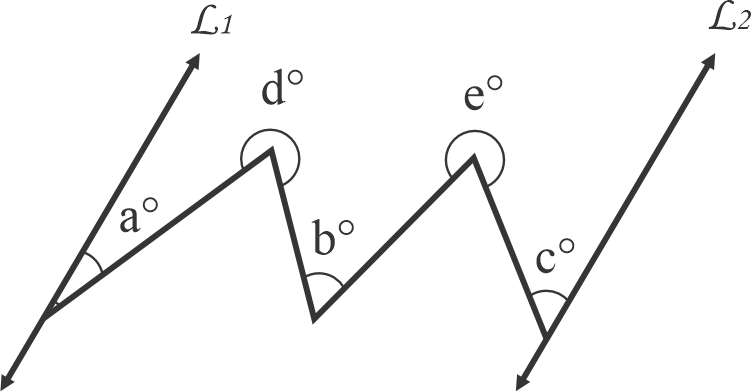
\includegraphics[width=4.5cm]{imagenes/general2024-I/etapa2/soc/geometria2g24-II.png}
	\end{center}
	
	
	\begin{enumerate}[label=\alph*)]
		\item $360^\circ$
		\item $450^\circ$
		\item $540^\circ$
		\item $600^\circ$
		\item $720^\circ$
	\end{enumerate}
	
	\textbf{Respuesta correcta:} e)
	
	\vspace{2mm}
	\textbf{Solucionario:}
	
	\begin{center}
		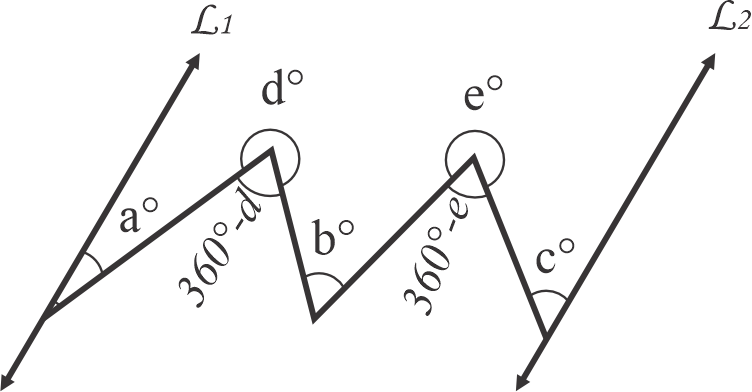
\includegraphics[width=4.5cm]{imagenes/general2024-I/etapa2/soc/geometria2g24-IIr.png}
	\end{center}
	
	De la figura se tiene:
	
	$a^\circ+b^\circ+c^\circ = 360^\circ-d^\circ+360^\circ-e^\circ$
	
	$a^\circ+b^\circ+c^\circ+d^\circ+e^\circ = $\fbox{$720^\circ$}
	
	
\end{enumerate}















\subsection*{Trigonometría}

\begin{enumerate}[resume]
	
	\item En el gráfico, halle $\tan \alpha$.
	
	\begin{center}
		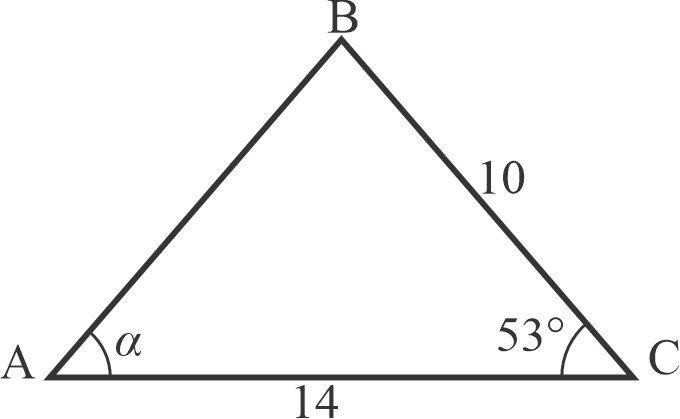
\includegraphics[width=4.5cm]{imagenes/general2024-I/etapa2/soc/trigo1g24-II.png}
	\end{center}
	\begin{enumerate}[label=\alph*)]
		\item 1
		\item $\dfrac{3}{2}$
		\item 2
		\item $\dfrac{3}{4}$
		\item $\dfrac{5}{4}$
	\end{enumerate}
	
	\textbf{Respuesta correcta:} a)
	
	\vspace{2mm}
	\textbf{Solucionario:}\\[1mm]
	\begin{center}
		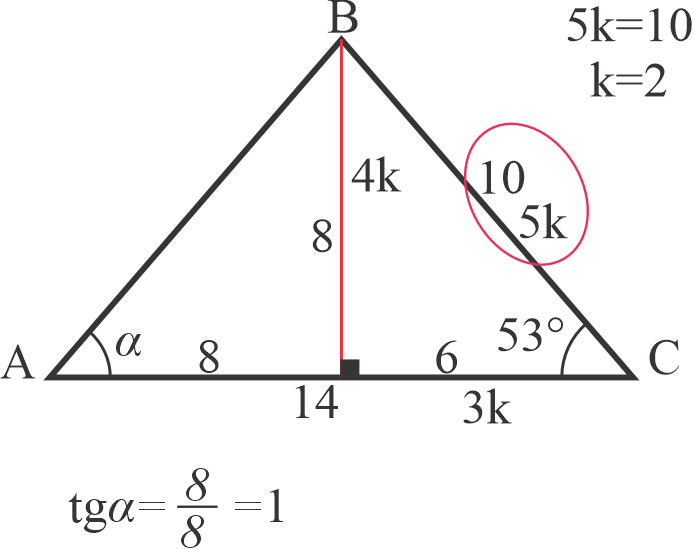
\includegraphics[width=0.4\textwidth]{imagenes/general2024-I/etapa2/soc/trigo1g24-IIr.png}
	\end{center}
	
	\vspace{6mm}
	
	
	
	
	
	\item Calcule el valor de:
	
	\[
	M=\dfrac{4\cos120^\circ-\tg135^\circ}{\sen330^\circ}
	\]
	
	\begin{enumerate}[label=\alph*)]
		\item 6
		\item 2
		\item -3
		\item 3
		\item -2
	\end{enumerate}
	
	\textbf{Respuesta correcta:} b)
	
	\vspace{2mm}
	\textbf{Solucionario:}\\[1mm]
	
	$
	M=\dfrac{4\cos120^\circ-\tg135^\circ}{\sen330^\circ}
	$
	
	$
	M=\dfrac{4\left(-\cos60^\circ\right)-\left(-\tg45^\circ\right)}{-\sen30^\circ}
	$
	
	$
	M=\dfrac{4\left(-\dfrac{1}{2}\right)+1}{-\dfrac{1}{2}}
	$
	
	$
	M=\dfrac{-2+1}{-\dfrac{1}{2}}=$\fbox{$2$}
	
	\vspace{6mm}
	
\end{enumerate}




\subsection*{Física}

\begin{enumerate}[resume]
	
	\item Una esfera de 50 kg se encuentra en equilibrio, tal como se muestra en la figura. Determine la fuerza de reacción en el punto B. Considere superficies lisas.  
	(g = 10 m/s²)
	
	\begin{center}
		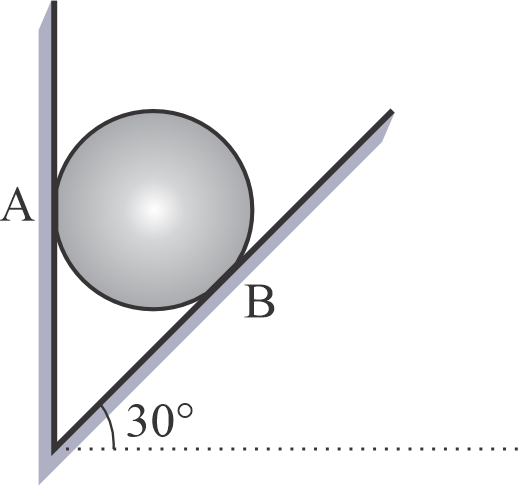
\includegraphics[width=0.3\textwidth]{imagenes/general2024-I/etapa2/soc/fisica1g24-II.png}
	\end{center}
	
	\begin{enumerate}[label=\alph*)]
		\item $\dfrac{3}{\sqrt{3}}$ kN
		\item $\dfrac{2}{\sqrt{3}}$ kN
		\item $\dfrac{\sqrt{3}}{2}$ kN
		\item $\dfrac{\sqrt{3}}{3}$ kN
		\item $\dfrac{\sqrt{2}}{3}$ kN
	\end{enumerate}
	
	\textbf{Respuesta correcta:} d)
	
	\textbf{Solucionario:}
	
	
	Del DCL  
	
	$W = 500\,N$
	
	comparando con  
	
	$K\sqrt{3} = 500\,N$
	
	$K = \dfrac{500}{\sqrt{3}}\,N$
	
	luego:
	
	$R_B = 2K = \dfrac{1000}{\sqrt{3}}\,N$
	
	$R_B = \dfrac{1000\sqrt{3}}{3}\,N =$ \fbox{$ \dfrac{\sqrt{3}}{3}\,kN$}
	
	
	
	
	
	
	
	
	\item José carga una mochila de 400 N de peso sobre su espalda al subir una colina de 30° de inclinación y recorre 40 m en un tiempo de 40 segundos a velocidad constante. Calcule la potencia desarrollada por José para llevar la mochila.
	
	\begin{enumerate}[label=\alph*)]
		\item 300 W
		\item 250 W
		\item 200 W
		\item 100 W
		\item 150 W
	\end{enumerate}
	
	\textbf{Respuesta correcta:} c)
	
	\textbf{Solucionario:}\\[1mm]
	
	
	\begin{center}
		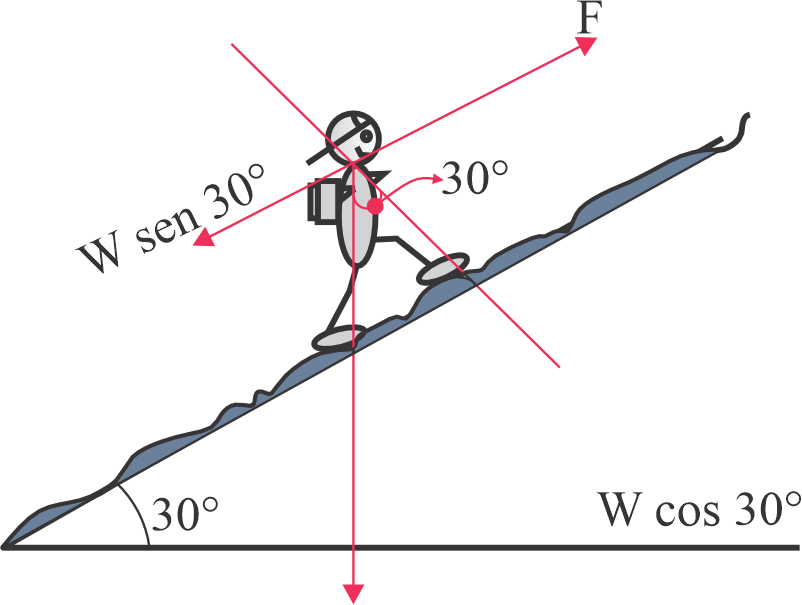
\includegraphics[width=4.5cm]{imagenes/general2024-I/etapa2/soc/fisica2g24-IIr.png}
	\end{center}
	
	\textbf{Solucionario:}
	
	$
	\begin{aligned}
		P &= \dfrac{W}{t} \\
		&= \dfrac{F\cdot d}{t} \\
		&= \dfrac{W\sen 30^\circ \cdot d}{t} \\
		&= \dfrac{400\left(\dfrac{1}{2}\right)(40)}{40} \\
		&=\fbox{ 200\,W}
	\end{aligned}
	$
	
\end{enumerate}







\subsection*{Química}

\begin{enumerate}[resume]
	\item Señale la alternativa que contiene una mezcla, una sustancia compuesta y un elemento, en ese orden.
	
	\begin{enumerate}[label=\Roman*.]
		\item Aire, ácido sulfúrico, agua destilada
		\item Oro de 18 kilates, cloruro de sodio, cobre
		\item Agua destilada, dióxido de carbono, cloro
		\item Agua potable, grafito, ozono
		\item Diamante, glucosa, aluminio.
	\end{enumerate}
	
	\begin{enumerate}[label=\alph*)]
		\item Solo IV
		\item III y IV
		\item Solo II
		\item Solo I
		\item II y IV
	\end{enumerate}
	
	\textbf{Respuesta correcta:} c)
	
	\vspace{2mm}
	\textbf{Solucionario:}\\[1mm]
	
	\begin{itemize}
		\item La mezcla es una reunión de 2 o más componentes, no se puede diferenciar sus componentes a simple vista. El oro de 18 kilates es una mezcla de oro y plata.
		\item Una sustancia compuesta es aquella sustancia formada por una sola clase de moléculas, siendo la molécula formada por átomos diferentes. El cloruro de sodio (NaCl) tiene 2 moléculas diferentes.
		\item Es un elemento químico que se encuentra en la naturaleza, como los metales nativos, ejemplo Cobre, Fierro, etc.)
	\end{itemize}
	
	\vspace{6mm}
	
	\item Señale las proposiciones verdaderas (V) o falsas (F) según corresponda sobre el efecto invernadero.
	
	\begin{enumerate}[label=\Roman*.]
		\item Es el fenómeno mediante el cual se evita que la totalidad de la energía emitida por la superficie terrestre, escape al espacio.
		\item Los gases de efecto invernadero son CO$_2$, CH$_4$, CCl$_2$F$_2$ entre los principales
		\item El gas que contribuye principalmente al efecto invernadero es el CO$_2$.
	\end{enumerate}
	
	\begin{enumerate}[label=\alph*)]
		\item VFV
		\item VVF
		\item VVV
		\item FVV
		\item FVF
	\end{enumerate}
	
	\textbf{Respuesta correcta:} c)
	
	\vspace{2mm}
	\textbf{Solucionario:}
	
	
	Los gases de efecto invernadero son CO$_2$, CH$_4$, CCl$_2$F$_2$ el principal es CO$_2$.
	
	\vspace{6mm}
	
	
\end{enumerate}



\subsection*{Biología y Anatomía}

\begin{enumerate}[resume]
	\item El epitelio simple cilíndrico ciliado se localiza en:
	\begin{enumerate}[label=\alph*)]
		\item Alveolos pulmonares
		\item Pelvis renal
		\item Conjuntiva ocular
		\item Trompas de falopio
		\item Vesícula seminal
	\end{enumerate}
	\textbf{Respuesta correcta:} d)
	
	\vspace{2mm}
	\textbf{Solucionario:}\\[1mm]
	El epitelio de las trompas de Falopio (u oviductos) presenta cilios en su superficie apical que facilitan el transporte del ovocito hacia el útero.
	
	
	\vspace{6mm}
	
	\item ¿Cuál es el polisacárido de reserva en algunos vegetales como el yacón y la alcachofa que está constituido por residuos de fructosa?
	\begin{enumerate}[label=\alph*)]
		\item Pectina
		\item Inulina
		\item Celulosa
		\item Almidón
		\item Ciclodextrina
	\end{enumerate}
	\textbf{Respuesta correcta:} b)
	
	\vspace{2mm}
	\textbf{Solucionario:}\\[1mm]
	La inulina es un fructosano (polímero de fructosa) que sirve como reserva energética en plantas de la familia Asteraceae, a diferencia del almidón que es polímero de glucosa.
	
	
	\vspace{6mm}
\end{enumerate}

\subsection*{Psicología y Filosofía}

\begin{enumerate}[resume]
	\item Si decimos que la mortalidad es algo común en todos los seres vivos, ¿qué operación del pensamiento estamos utilizando?
	\begin{enumerate}[label=\alph*)]
		\item Abstracción
		\item Síntesis
		\item Análisis
		\item Comparación
		\item Generalización
	\end{enumerate}
	\textbf{Respuesta correcta:} e)
	
	\vspace{2mm}
	\textbf{Solucionario:}\\[1mm]
	La generalización es la operación mental que consiste en atribuir una característica observada en elementos particulares a todo un grupo, clase o especie.
	
	\vspace{6mm}
	
	\item Existen pacientes que sufren de amnesia, los cuales a veces son incapaces de recordar un número telefónico, una dirección o el nombre de una persona, pero sí pueden recordar cómo resolver rompecabezas complejos en un tiempo normal, lo cual sería un indicador de que no se encuentra dañada la memoria:
	\begin{enumerate}[label=\alph*)]
		\item semántica.
		\item procedimental.
		\item episódica.
		\item declarativa.
		\item transitoria.
	\end{enumerate}
	\textbf{Respuesta correcta:} b)
	
	\vspace{2mm}
	\textbf{Solucionario:}\\[1mm]
	La memoria procedimental es la encargada de almacenar información sobre procedimientos y habilidades motoras (el "saber cómo"). Esta memoria suele ser más resistente al daño que la declarativa.
	
	\vspace{6mm}
	
	\item En relación con la esencia humana, señale verdad (V) o falsedad (F) de los enunciados.\\
	I. Según Aristóteles, el hombre fuera de la sociedad no podría vivir.\\
	II. Para el maestro de Aristóteles, el hombre nunca muere.\\
	III. Cassire manifiesta que el hombre, antes que se guíe por su razón, se guiaría por su cultura.\\
	IV. Según Nietzsche, el hombre ha roto con su estado natural.\\
	V. Según Cassire, el hombre por naturaleza es un animal simbólico.
	\begin{enumerate}[label=\alph*)]
		\item V V V F V
		\item F F F F V
		\item F V V F V
		\item V V V V F
		\item F F V V V
	\end{enumerate}
	\textbf{Respuesta correcta:} d)
	
	\vspace{2mm}
	\textbf{Solucionario:}\\[1mm]
	I(V): El hombre es un \textit{zoon politikon}. \\
	II(V): Platón postula la inmortalidad del alma. \\
	III(V): La cultura media la relación del hombre con el mundo. \\
	IV(V): Nietzsche afirma que la civilización ha "enfermado" al hombre al separarlo de sus instintos naturales.\\ 
	V(F): Para Cassirer, el simbolismo es una función funcional de la cultura, no un rasgo de la "naturaleza" biológica previa.\\
	
	\vspace{6mm}
	
	\item Determine aquella disciplina en donde nos preguntamos si lo primero es la materia o la idea.
	\begin{enumerate}[label=\alph*)]
		\item Ontología
		\item Epistemología
		\item Axiología
		\item Ética
		\item Gnoseología
	\end{enumerate}
	\textbf{Respuesta correcta:} a)
	
	\vspace{2mm}
	\textbf{Solucionario:}\\[1mm]
	La Ontología (estudio del ser) aborda el problema fundamental de la filosofía: la primacía entre el ser (materia) y el pensar (idea/conciencia).
	
	\vspace{6mm}
\end{enumerate}




\subsection*{Geografía}

\begin{enumerate}[resume]
	\item La capa de la atmósfera del planeta Tierra donde se producen la mayor parte de los fenómenos (vientos, lluvias, nubes, etc.), se denomina:
	\begin{enumerate}[label=\alph*)]
		\item Tropósfera
		\item Termósfera
		\item Estratósfera
		\item Mesósfera
		\item Exósfera
	\end{enumerate}
	\textbf{Respuesta correcta:} a)
	
	\vspace{2mm}
	\textbf{Solucionario:}\\[1mm]
	La tropósfera es la capa en contacto con la superficie terrestre; en ella ocurre la dinámica meteorológica debido a la mayor densidad de gases y vapor de agua.
	
	\vspace{6mm}
	
	\item En los problemas ambientales del Perú, una de las consecuencias directas de la mala disposición de los residuos sólidos es:
	\begin{enumerate}[label=\alph*)]
		\item el gasto económico para solucionar los daños
		\item el conflicto de las autoridades con la población
		\item la corrupción vinculada al manejo de residuos sólidos
		\item la legislación inapropiada
		\item el daño a la salud y al ambiente
	\end{enumerate}
	\textbf{Respuesta correcta:} e)
	
	\vspace{2mm}
	\textbf{Solucionario:}\\[1mm]
	La acumulación de basura a cielo abierto genera focos infecciosos, proliferación de vectores y contaminación de suelos y fuentes de agua, impactando directamente en el ecosistema y la salud pública.
	
	\vspace{6mm}
	
	\item El crecimiento demográfico en los países en que los recursos no han crecido en la misma proporción, es uno de los factores que explica la situación de:
	\begin{enumerate}[label=\alph*)]
		\item la política.
		\item la comunidad nativa.
		\item la pobreza.
		\item los recursos naturales.
		\item los patrones de consumo.
	\end{enumerate}
	\textbf{Respuesta correcta:} c)
	
	\vspace{2mm}
	\textbf{Solucionario:}\\[1mm]
	Según la teoría malthusiana y visiones socioeconómicas modernas, cuando la población crece a un ritmo mayor que la capacidad de producción de recursos y servicios, se agudizan las condiciones de pobreza.
	
	\vspace{6mm}
	
	\item Uno de los efectos del cambio climático en la Tierra es:
	\begin{enumerate}[label=\alph*)]
		\item la disminución del nivel del mar
		\item el incremento de las enfermedades tropicales
		\item la disminución de los fenómenos naturales
		\item el aumento de los recursos naturales
		\item la disminución de la contaminación
	\end{enumerate}
	\textbf{Respuesta correcta:} b)
	
	\vspace{2mm}
	\textbf{Solucionario:}\\[1mm]
	El aumento de la temperatura global permite que vectores (como mosquitos) expandan su hábitat hacia zonas antes frías, incrementando la incidencia de enfermedades como el dengue o la malaria.
	
	\vspace{6mm}
\end{enumerate}

\subsection*{Historia}

\begin{enumerate}[resume]
	\item A partir del periodo de la posguerra con Chile y hasta las primeras décadas del siglo XX, el sector ganadero alcanzó un gran auge incorporándose al ciclo económico de exportación. En el sur peruano, las ciudades de Arequipa, Puno y Cusco experimentaron una creciente prosperidad gracias al:
	\begin{enumerate}[label=\alph*)]
		\item apoyo gubernamental.
		\item sistema de gamonales.
		\item desarrollo de carreteras.
		\item control tributario.
		\item sistema de ferrocarriles.
	\end{enumerate}
	\textbf{Respuesta correcta:} e)
	
	\vspace{2mm}
	\textbf{Solucionario:}\\[1mm]
	La construcción del Ferrocarril del Sur facilitó el transporte de lana (alpaca y oveja) desde el altiplano hacia el puerto de Mollendo para su exportación a Inglaterra, dinamizando la economía regional.
	
	\vspace{6mm}
	
	\item El gran éxito económico de la era del guano en el Perú tuvo como base científica las investigaciones sobre las propiedades fertilizantes del guano de islas que realizaron diversos estudiosos, entre ellos destaca el naturalista peruano:
	\begin{enumerate}[label=\alph*)]
		\item Mariano de Rivero y Ustariz.
		\item Manuel Ascencio Segura.
		\item Mariano Paz Soldan.
		\item Juan Bautista Dueñas.
		\item Pedro Paulet.
	\end{enumerate}
	\textbf{Respuesta correcta:} a)
	
	\vspace{2mm}
	\textbf{Solucionario:}\\[1mm]
	Mariano Eduardo de Rivero y Ustariz fue un prominente científico peruano que realizó los primeros análisis químicos del guano, demostrando su alto valor como abono orgánico en el mercado europeo.
	
	\vspace{6mm}
	
	\item A partir de 1955, la OTAN tuvo como contraparte militar al:
	\begin{enumerate}[label=\alph*)]
		\item gobierno soviético.
		\item Plan Molotov.
		\item COMECON.
		\item Plan Marshall.
		\item Pacto de Varsovia.
	\end{enumerate}
	\textbf{Respuesta correcta:} e)
	
	\vspace{2mm}
	\textbf{Solucionario:}\\[1mm]
	El Pacto de Varsovia fue una alianza de defensa mutua firmada en 1955 por los países del bloque socialista (liderados por la URSS) en respuesta al ingreso de Alemania Occidental a la OTAN.
	
	\vspace{6mm}
	
	\item El alto órgano administrativo para el gobierno de América que nombraba al Virrey y al final de su mandato lo sometía a un juicio de residencia y que además señalaba los lineamientos de la política virreinal fue:
	\begin{enumerate}[label=\alph*)]
		\item la Casa de Contratación de Sevilla
		\item la Intendencia
		\item la Real Audiencia
		\item la Corona Española
		\item el Consejo de Indias
	\end{enumerate}
	\textbf{Respuesta correcta:} e)
	
	\vspace{2mm}
	\textbf{Solucionario:}\\[1mm]
	El Real y Supremo Consejo de Indias tenía funciones legislativas, ejecutivas y judiciales; entre ellas, la selección de altos funcionarios y la fiscalización mediante el juicio de residencia.
	
	\vspace{6mm}
\end{enumerate}


\subsection*{Educación Cívica}

\begin{enumerate}[resume]
	\item Según la Constitución Política de la República del Perú, se suspende el ejercicio de la Presidencia de la República:
	\begin{enumerate}[label=\alph*)]
		\item cuando sale del territorio nacional sin permiso del Congreso.
		\item por su permanente incapacidad moral y física.
		\item cuando ha sido destituido por infracciones contra la Constitución.
		\item por incapacidad temporal del Presidente, declarado por el Congreso.
		\item cuando se acepta su renuncia por el congreso.
	\end{enumerate}
	\textbf{Respuesta correcta:} d)
	
	\vspace{2mm}
	\textbf{Solucionario:}\\[1mm]
	El artículo 114 de la Constitución establece las causales de suspensión, diferenciándolas de la vacancia (incapacidad permanente). La suspensión es temporal y debe ser declarada por el Legislativo.
	
	\vspace{6mm}
	
	\item Puede presentar la acción de inconstitucionalidad:
	\begin{enumerate}[label=\alph*)]
		\item el Consejo de Ministros.
		\item el 15 \% del número legal de Congresistas.
		\item el Defensor del Pueblo.
		\item la Junta de Fiscales.
		\item 2000 ciudadanos con firmas comprobadas por el JNE.
	\end{enumerate}
	\textbf{Respuesta correcta:} c)
	
	\vspace{2mm}
	\textbf{Solucionario:}\\[1mm]
	Según el artículo 203 de la Constitución, el Defensor del Pueblo tiene legitimidad para interponer esta acción ante el Tribunal Constitucional para garantizar que las leyes no vulneren la Carta Magna.
	
	\vspace{6mm}
	
	\item Una de las atribuciones del Presidente de la República según la Constitución es:
	\begin{enumerate}[label=\alph*)]
		\item velar por el respeto de la Constitución y de las leyes.
		\item ejercer el derecho de amnistía.
		\item aprobar tratados de conformidad con la Constitución.
		\item convocar a elecciones generales, parlamentarias, regionales y locales.
		\item aprobar la demarcación territorial que proponga el Poder Ejecutivo.
	\end{enumerate}
	\textbf{Respuesta correcta:} d)
	
	\vspace{2mm}
	\textbf{Solucionario:}\\[1mm]
	De acuerdo al Artículo 118 de la Constitución Política del Perú (inciso 5), el Presidente tiene la facultad de convocar a los procesos electorales en todos los niveles de gobierno. La amnistía es facultad del Congreso, y la opción "a" es un deber general pero la "d" es la atribución técnica específica.
	
	\vspace{6mm}
	
	\item La legislación peruana, señala que la emisión de monedas y billetes es una facultad exclusiva del \rule{1.5cm}{0.4pt} y se realiza a través \rule{1.5cm}{0.4pt}
	\begin{enumerate}[label=\alph*)]
		\item Estado - de la SBS.
		\item BCR - del Estado.
		\item Estado - del BCR.
		\item MEF - del BCR.
		\item Estado - del MEF.
	\end{enumerate}
	\textbf{Respuesta correcta:} c)
	
	\vspace{2mm}
	\textbf{Solucionario:}\\[1mm]
	El Estado peruano ejerce el monopolio de la emisión de dinero a través de su organismo autónomo, el Banco Central de Reserva (BCR), encargado de preservar la estabilidad monetaria.
	
	\vspace{6mm}
\end{enumerate}

\subsection*{Economía}

\begin{enumerate}[resume]
	\item En el Perú, existe un grupo de bancos como el Banco de Crédito del Perú, el Banco Continental, Interbank, etc.; estos bancos son supervisados por la superintendencia de Banca, Seguros y AFP. Según clasificación de la empresa de acuerdo a la propiedad, estos bancos se clasifican como empresas:
	\begin{enumerate}[label=\alph*)]
		\item sociedades anónimas cerradas.
		\item públicas.
		\item sociedades en comandita.
		\item privadas.
		\item mixtas.
	\end{enumerate}
	\textbf{Respuesta correcta:} d)
	
	\vspace{2mm}
	\textbf{Solucionario:}\\[1mm]
	Son empresas privadas porque sus activos y capital pertenecen a inversionistas particulares (personas naturales o jurídicas), con el objetivo de generar rentabilidad para sus dueños.
	
	\vspace{6mm}
	
	\item Ana, para obtener el título de economista, está realizando una tesis acerca del mercado de valores peruanos y observa que en este mercado se vende y compra principalmente:
	\begin{enumerate}[label=\alph*)]
		\item cheques.
		\item depósitos de ahorro.
		\item acciones y bonos.
		\item letras de cambio.
		\item bonos soberanos.
	\end{enumerate}
	\textbf{Respuesta correcta:} c)
	
	\vspace{2mm}
	\textbf{Solucionario:}\\[1mm]
	El mercado de valores (como la Bolsa de Valores de Lima) se especializa en la intermediación directa a través de títulos de participación (acciones) y títulos de deuda (bonos).
	
	\vspace{6mm}
	
	\item Tener una baja tasa de inflación, además de un tipo de cambio estable, está directamente relacionado con un objetivo de la política económica denominado:
	\begin{enumerate}[label=\alph*)]
		\item desarrollo económico.
		\item estabilidad económica.
		\item pleno empleo.
		\item eficiencia distributiva.
		\item equilibrio externo.
	\end{enumerate}
	\textbf{Respuesta correcta:} b)
	
	\vspace{2mm}
	\textbf{Solucionario:}\\[1mm]
	La estabilidad económica se refiere al mantenimiento del equilibrio macroeconómico, evitando crisis inflacionarias o devaluaciones bruscas que afecten la inversión y el consumo.
	
	\vspace{6mm}
	
	\item Una reducción de la demanda de carne de pollo puede deberse a:
	\begin{enumerate}[label=\alph*)]
		\item un incremento del precio de la carne de res.
		\item una variación de los impuestos.
		\item la disminución de su precio.
		\item una mejora de los ingresos del consumidor.
		\item una disminución del precio de la carne de pescado.
	\end{enumerate}
	\textbf{Respuesta correcta:} e)
	
	\vspace{2mm}
	\textbf{Solucionario:}\\[1mm]
	El pescado es un bien sustituto del pollo. Si el precio del sustituto baja, los consumidores dejarán de comprar pollo para adquirir pescado, reduciendo así la demanda del primero.
	
	\vspace{6mm}
\end{enumerate}


\subsection*{Comunicación}

\begin{enumerate}[resume]
	\item Era de postura mediana, de anchas espaldas, fuertemente labrado y músculos. El cuerpo estaba deformado por el trabajo, caminaba con la cabeza erguida, la espalda combada y el vientre hacia adelante.\\
	\\
	¿A qué tipo de texto corresponde el fragmento?
	\begin{enumerate}[label=\alph*)]
		\item Narrativo
		\item Expositivo
		\item Descriptivo
		\item Argumentativo
		\item Instructivo
	\end{enumerate}
	\textbf{Respuesta correcta:} c)
	
	\vspace{2mm}
	\textbf{Solucionario:}\\[1mm]
	El fragmento se centra en detallar las características físicas de un sujeto (prosopografía), lo cual es la función principal del texto descriptivo.
	
	\vspace{6mm}
	
	\item El licenciado Jorge, director de su escuela profesional, decide felicitar al coordinador de responsabilidad social por haber participado en la parada universitaria.\\
	\\
	¿Qué tipo de documento redactará?
	\begin{enumerate}[label=\alph*)]
		\item Informe
		\item Solicitud
		\item Acta
		\item Memorando
		\item Oficio
	\end{enumerate}
	\textbf{Respuesta correcta:} e)
	
	\vspace{2mm}
	\textbf{Solucionario:}\\[1mm]
	El oficio es el documento utilizado por autoridades para comunicaciones oficiales (felicitaciones, agradecimientos, gestiones) entre dependencias o hacia el exterior.
	
	\vspace{6mm}
	
	\item La telenovela es un género de la televisión que narra historias ficticias.\\
	\\
	El enunciado:
	\begin{enumerate}[label=\alph*)]
		\item relata un hecho.
		\item defiende una opinión.
		\item explica un fenómeno.
		\item describe un objeto.
		\item reproduce una interacción verbal.
	\end{enumerate}
	\textbf{Respuesta correcta:} c)
	
	\vspace{2mm}
	\textbf{Solucionario:}\\[1mm]
	El enunciado tiene una función informativa o referencial; busca definir o explicar qué es la telenovela dentro del contexto televisivo.
	
	\vspace{6mm}
	
	\item Consiste en organizar información relevante alrededor de una idea principal o postura que aparece en un texto. Permite desarrollar habilidades de manejo de información, análisis de situaciones y pensamiento crítico.
	\begin{enumerate}[label=\alph*)]
		\item Espina de Ishikawa
		\item Mapa semántico
		\item Cruz categorial
		\item Diagrama de flujo
		\item Mapa conceptual
	\end{enumerate}
	\textbf{Respuesta correcta:} c)
	
	\vspace{2mm}
	\textbf{Solucionario:}\\[1mm]
	La cruz categorial es un organizador visual que permite analizar un tema central (ubicado en el centro) relacionándolo con sus causas, consecuencias, argumentos y propósitos.
	
	\vspace{6mm}
\end{enumerate}

\subsection*{Literatura}

\begin{enumerate}[resume]
	\item ¿Cómo termina la novela "El viejo y el mar" de Hemingway?
	\begin{enumerate}[label=\alph*)]
		\item Manolín recibe a Santiago en la playa y admira el espinazo del pez aguja, que es todo lo que quedó.
		\item Santiago despierta en su cabaña, pues todo había sido un sueño.
		\item Santiago y Manolín parten de nuevo para superar la hazaña del viejo.
		\item Santiago muere en los arenales del mar.
		\item Una mujer comenta acerca del espinazo del Pez.
	\end{enumerate}
	\textbf{Respuesta correcta:} a)
	
	\vspace{2mm}
	\textbf{Solucionario:}\\[1mm]
	Tras la lucha contra los tiburones, Santiago llega a la orilla solo con el esqueleto del gran pez. Su leal aprendiz, Manolín, lo recibe y lo cuida, reconociendo su valor.
	
	\vspace{6mm}
	
	\item Se constituye como el movimiento literario más importante de España se caracteriza por su hermetismo, uso recargado de adornos estéticos y complejos en su composición. ejm. El ingenioso don Quijote de la Mancha.
	\begin{enumerate}[label=\alph*)]
		\item Neo clasismo
		\item Realismo
		\item Barroquismo
		\item Costumbrismo
		\item Romanticismo
	\end{enumerate}
	\textbf{Respuesta correcta:} c)
	
	\vspace{2mm}
	\textbf{Solucionario:}\\[1mm]
	El Barroco español destaca por la sofisticación formal (culteranismo y conceptismo), el contraste y la visión pesimista de la realidad, presente en la madurez de Cervantes.
	
	\vspace{6mm}
	
	\item ¿Qué figura literaria se destaca en los versos de "La vida es un sueño"?\\
	\\
	Hace el arroyo, culebra\\
	que entre flores se desata\\
	entre las flores se quiebra
	\begin{enumerate}[label=\alph*)]
		\item símil
		\item metonimia
		\item metáfora
		\item hipérbole
		\item hipérbaton
	\end{enumerate}
	\textbf{Respuesta correcta:} c)
	
	\vspace{2mm}
	\textbf{Solucionario:}\\[1mm]
	Se emplea la metáfora al identificar al arroyo directamente con una "culebra" por su forma serpenteante, sin usar nexos como "parece" o "como".
	
	\vspace{6mm}
	
	\item "Los miserables" y "Nuestra Señora de París" obras de Víctor Hugo, pertenecen al género:
	\begin{enumerate}[label=\alph*)]
		\item épico.
		\item lírico.
		\item narrativo.
		\item expositivo.
		\item dramático.
	\end{enumerate}
	\textbf{Respuesta correcta:} c)
	
	\vspace{2mm}
	\textbf{Solucionario:}\\[1mm]
	Al ser novelas que relatan una secuencia de hechos a través de un narrador en prosa, se ubican dentro del género narrativo moderno.
	
	\vspace{6mm}
\end{enumerate}











\subsection*{Razonamiento Matemático}

\begin{enumerate}[resume]
	
	\item En el gráfico, se muestran dos cuadrados mágicos aditivos de $3 \times 3$. Calcule $A+B+C-(D+E+F)$
	
	\begin{center}
		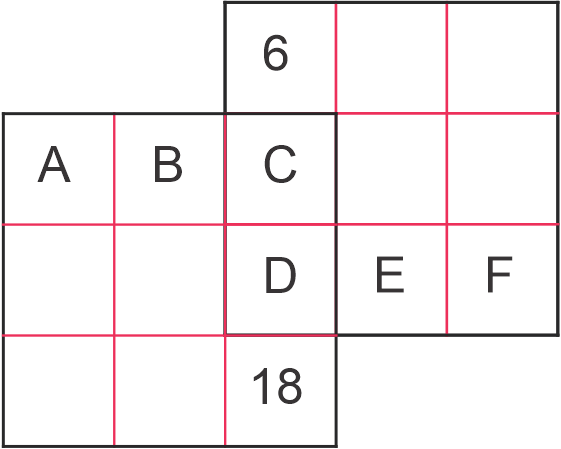
\includegraphics[width=3.5cm]{imagenes/general2024-I/etapa2/soc/rm1g24-II.png}
	\end{center}
	
	\begin{enumerate}[label=\alph*)]
		\item 18
		\item 12
		\item 24
		\item 9
		\item 8
	\end{enumerate}
	\textbf{Respuesta correcta:} b)
	
	\vspace{2mm}
	
	\textbf{Solucionario:}


	De la figura y el cuadrado mágico de la izquierda:
	
	\begin{equation*}
		A + B = D + 18 \quad \Rightarrow \quad A + B - D = 18 \quad \dots (I)
	\end{equation*}
	
	De la figura y el cuadrado mágico de la derecha:
	\begin{equation*}
		G + C = E + F \quad \Rightarrow \quad C - E - F = -G \quad \dots (II)
	\end{equation*}
	Sumando (I) y (II):
	\begin{align*}
		A + B - D + C - E - F &= 18 - 6 \\
		A + B + C - D - E - F &= 12 \\
		A + B + C - (D + E + F) &= 12
	\end{align*}
	
	
	
	
	
	\vspace{6mm}
	
	\item Paula recomendada para el manejo de dinero, recibió 100 billetes de $S/ 20$, $S/ 50$ y $S/ 100$, y el monto recibido es de $S/ 7300$. El número de billetes de $S/ 20$ es la mitad de los de $S/ 50$. ¿Cuál es el número de billetes de $S/ 100$?
	\begin{enumerate}[label=\alph*)]
		\item 53
		\item 55
		\item 50
		\item 57
		\item 65
	\end{enumerate}
	\textbf{Respuesta correcta:} b)
	
	\vspace{2mm}
	
	\textbf{Solucionario:}
	
	El total de billetes es 100
	\begin{center}
		\begin{tabular}{|c|c|c|c|c|}
			\hline
			& $S/. 20$ & $S/. 50$ & $S/. 100$ & TOTAL \\ \hline
			\# de billetes & $x$ & $2x$ & $100 - 3x$ & $100$ \\ \hline
			Monto & $20x$ & $50(2x)$ & $100(100 - 3x)$ & $7300$ \\ \hline
		\end{tabular}
	\end{center}
	
	Planteando:
	\begin{align*}
		2x + 5(2x) + 10(100 - 3x) &= 730 \\
		18x = 270 \quad \Rightarrow \quad &x = 15
	\end{align*}
	
	$\therefore$ \# de billetes de $S/. 100$
	\begin{equation*}
		\text{es } 100 - 3x = 100 - 3(15) = \fbox{55}
	\end{equation*}
	
	
	
	
	\vspace{6mm}
	
	\item Dos relojes se sincronizan a las 12 del mediodía. Si uno de ellos se atrasa 12 minutos cada hora con respecto a otro, ¿cuánto tiempo transcurrirá hasta que ambos relojes marquen la misma hora?
	\begin{enumerate}[label=\alph*)]
		\item 2,0 días
		\item 1,5 días
		\item 2,5 días
		\item 3,5 días
		\item 3,0 días
	\end{enumerate}
	\textbf{Respuesta correcta:} c)
	
	\vspace{2mm}
	
	\textbf{Solucionario:}
	
	Dato: Uno de los relojes se atrasa 12 minutos por cada hora.
	
	\begin{center}
		\begin{tabular}{c|c}
			Se atrasa & $1 \text{ h.}$ \\ \hline
			$12 \text{ min}$ & $60 \text{ h}$ \\
			$720 \text{ min}$ & 
		\end{tabular}
	\end{center}
	
	$\hookrightarrow$ Se debe atrasar $720$ minutos para que marque la misma hora.
	
	\begin{equation*}
		\dfrac{720}{12} = 60
	\end{equation*}
	
	$60 \text{ h.}$ es $2,5$ días.
	
	$\therefore$ Ambos relojes volverán a marcar la misma hora dentro de \fbox{$2,5$} días.
	
	
	\item Calcule el área de la región sombreada, donde los arcos son de circunferencia
	
	
	\begin{center}
		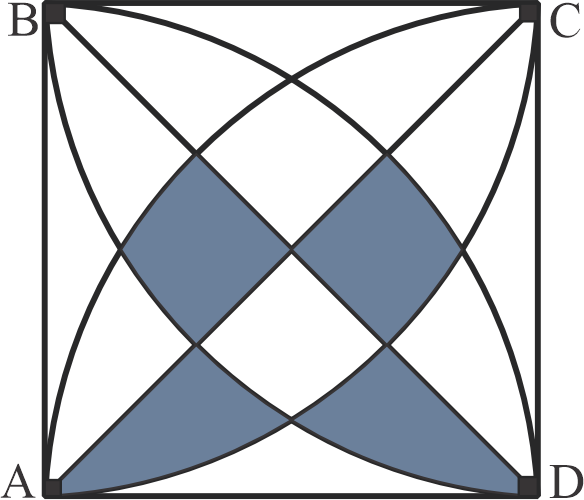
\includegraphics[width=0.3\textwidth]{imagenes/general2024-I/etapa2/soc/rm4g24-II.png}
	\end{center}
	
	\begin{enumerate}[label=\alph*)]
		\item $2(\pi-4)u^2$
		\item $3(2\pi-1)u^2$
		\item $6(\pi-2)u^2$
		\item $4(\pi-2)u^2$
		\item $5(\pi-4)u^2$
	\end{enumerate}	
	\textbf{Respuesta correcta:} d)
	
	\vspace{2mm}
	\textbf{Solucionario:}
	
	\begin{center}
		\begin{minipage}{0.45\textwidth}
			\begin{minipage}{0.45\textwidth}
				\centering
				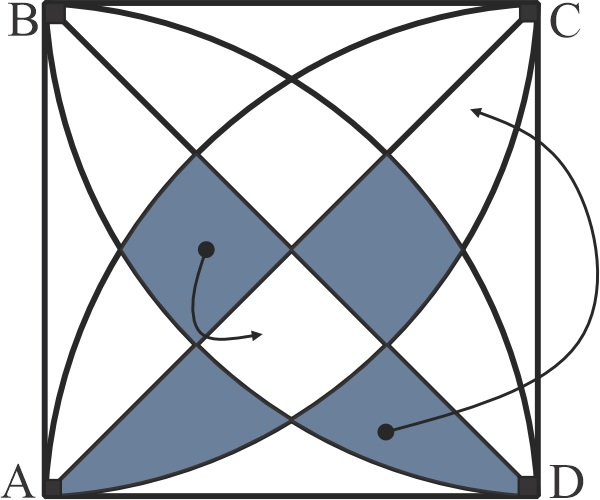
\includegraphics[width=3.5cm]{imagenes/general2024-I/etapa2/soc/rm4g24-IIr.png}
			\end{minipage}
			
			\vspace{6mm}
		\end{minipage}
		\hfill
		\begin{minipage}{0.45\textwidth}
			\centering
			S= Área de la cuarta parte de una circunferencia  menos al área de un triángulo\\
			
			$=\dfrac{\pi 4^2}{4}-\dfrac{4 \text{x} 4}{2}$\\
			
			$= 4 \pi -8$\\
			
			=\fbox{$4(\pi -2)u^2$}

		\end{minipage}
	\end{center}
	
	
	
	
	\item Halle el total de triángulos en la figura mostrada.
	
	\begin{center}
		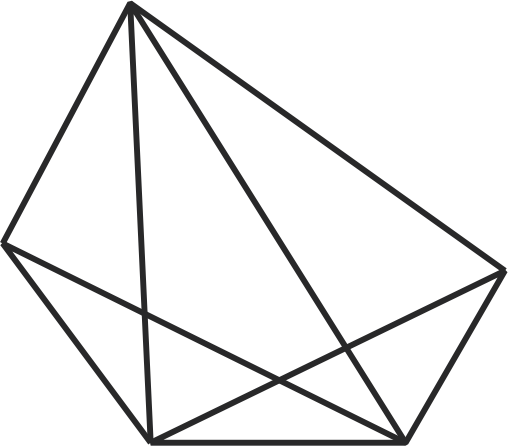
\includegraphics[width=0.3\textwidth]{imagenes/general2024-I/etapa2/soc/rm5g24-II.png}
	\end{center}
	
	
	\begin{enumerate}[label=\alph*)]
		\item 14
		\item 10
		\item 22
		\item 18
		\item 20
	\end{enumerate}
	\textbf{Respuesta correcta:} e)
	
	\vspace{2mm}
	\textbf{Solucionario:}
	
	Contando por regiones: 
	
	De 1 región: 1, 2, 3, 4, 5, 6, 7 $\rightarrow$ 7 
	
	De 2 regiones: 12, 23, 34, 45, 56, 67, 3X, 5X $\rightarrow$ 8 
	
	De 3 regiones: 234, 456, 1X5, 3X7 $\rightarrow$ 4 
	
	De 4 regiones: 345X $\rightarrow$ 1 
	
	Total = $7 + 8 + 4 + 1 = $\fbox{$20$}
	
	
	
	\vspace{6mm}
	
	\item Un estudiante tiene que resolver solamente 8 preguntas de 10 en un examen. ¿Cuántas maneras de escoger las preguntas tiene el estudiante?
	\begin{enumerate}[label=\alph*)]
		\item 10
		\item 35
		\item 45
		\item 25
		\item 20
	\end{enumerate}
	\textbf{Respuesta correcta:} c)
	
	\vspace{2mm}
	\textbf{Solucionario:}
	
	Es una combinatoria ya que no importa el orden de selección: 
	
	$C_{8}^{10} = \dfrac{10!}{(10-8)! \cdot 8!} = \dfrac{10 \times 9 \times 8!}{2! \cdot 8!} =$\fbox{$ 45$}
	
	\vspace{6mm}
	
	
	
	\vspace{6mm}
	
\end{enumerate} 	












































\subsection*{Razonamiento Verbal}

\begin{enumerate}[resume]
	\item En la palabra taquigrafía, la raíz griega \textit{taqui} significa:
	\begin{enumerate}[label=\alph*)]
		\item veloz.
		\item palabra.
		\item escritura.
		\item digitar.
		\item símbolos.
	\end{enumerate}
	\textbf{Respuesta correcta:} a)
	
	\vspace{2mm}
	\textbf{Solucionario:}\\[1mm]
	La raíz griega \textit{tachys} significa "rápido" o "veloz". Por lo tanto, la taquigrafía es el método de escritura rápida mediante signos y abreviaturas.
	
	\vspace{6mm}
	
	\item Julio Ramón Ribeyro - La tentación del fracaso (Diario): "¡Diablos! Si las últimas treinta o cuarenta novelas que he tratado de leer no las he terminado, es porque deben tener algún defecto, algo que les impiden colmar mis expectativas."\\
	\\
	¿A qué se deben las lecturas inconclusas del autor?
	\begin{enumerate}[label=\alph*)]
		\item A sus limitaciones académicas.
		\item Al estilo particular de la prosa.
		\item A la diversidad de los temas.
		\item A lo defectuoso de las novelas leídas.
		\item Al exagerado gusto Literario del autor.
	\end{enumerate}
	\textbf{Respuesta correcta:} d)
	
	\vspace{2mm}
	\textbf{Solucionario:}\\[1mm]
	El autor indica explícitamente que la razón por la que no termina las novelas es porque estas "deben tener algún defecto" que impide que cumplan sus expectativas.
	
	\vspace{6mm}
	
	\item Complete la oración:\\
	\\
	La vocación es el \rule{2cm}{0.4pt} íntimo que siente una persona hacia un tipo del \rule{2cm}{0.4pt}.
	\begin{enumerate}[label=\alph*)]
		\item dilema - actividad
		\item objetivo - profesión
		\item impulso - quehacer
		\item interés - accionar
		\item acto - labor
	\end{enumerate}
	\textbf{Respuesta correcta:} c)
	
	\vspace{2mm}
	\textbf{Solucionario:}\\[1mm]
	La palabra "impulso" se ajusta a la naturaleza interna de la vocación, mientras que "quehacer" se refiere a la actividad o tarea a la que uno se dedica.
	
	\vspace{6mm}
	
	\item El sinónimo de SINDÉRESIS es:
	\begin{enumerate}[label=\alph*)]
		\item acentuación.
		\item resumen.
		\item omisión.
		\item interés.
		\item juicio.
	\end{enumerate}
	\textbf{Respuesta correcta:} e)
	
	\vspace{2mm}
	\textbf{Solucionario:}\\[1mm]
	La sindéresis es la capacidad de juzgar rectamente o tener buen sentido, por lo que su sinónimo más preciso es "juicio".
	
	\vspace{6mm}
	
	\item Identifique el par analógico:\\
	\\
	DISIPACIÓN : GASTAR ::
	\begin{enumerate}[label=\alph*)]
		\item verborrea : hablar.
		\item tempestad : llover.
		\item carrera : trasladar.
		\item negligencia : actuar.
		\item apetito : comer.
	\end{enumerate}
	\textbf{Respuesta correcta:} a)
	
	\vspace{2mm}
	\textbf{Solucionario:}\\[1mm]
	La relación es de exceso o intensidad. Disipación es el gasto excesivo y desmedido, así como la verborrea es el hablar excesivo y redundante.
	
	\vspace{6mm}
	
	\item \textbf{PLAN DE REDACCIÓN}\\
	\\
	\textbf{Importancia de la sintaxis}
	\begin{itemize}[label={}]
		\item I. Etimológicamente, sintaxis quiere decir con orden.
		\item II. El dominio de la sintaxis influye en el orden del pensamiento.
		\item III. La sintaxis es parte de la gramática que enseña a ordenar las palabras para que el sentido de la oración sea completo.
		\item IV. El maestro hará ver que los pensamientos no funcionan por medio de palabras aisladas, sino palabras relacionadas unas con otras.
	\end{itemize}
	\begin{enumerate}[label=\alph*)]
		\item I - II - IV - III
		\item III - II - I - IV
		\item III - I - II - IV
		\item I - III - II - IV
		\item I - III - IV - II
	\end{enumerate}
	\textbf{Respuesta correcta:} d)
	
	\vspace{2mm}
	\textbf{Solucionario:}\\[1mm]
	El orden lógico comienza con la etimología (I), sigue con la definición gramatical (III), continúa con la importancia intelectual o cognitiva (II) y finaliza con la aplicación práctica en el aula (IV).
	
	\vspace{6mm}
\end{enumerate}


\subsection*{Inglés}

\begin{enumerate}[resume]
	\item Choose one alternative that it has one adverb of possibility.
	\begin{enumerate}[label=\alph*)]
		\item I need to call to my teacher.
		\item In my free time I fix cellphones.
		\item Maybe he is a lawyer.
		\item She has dread to go at the hospital.
		\item He like to stay in home.
	\end{enumerate}
	\textbf{Respuesta correcta:} c)
	
	\vspace{2mm}
	\textbf{Solucionario:}\\[1mm]
	La palabra "Maybe" (tal vez/quizás) es un adverbio de posibilidad que se utiliza para indicar que algo es probable pero no seguro. Las demás alternativas son oraciones enunciativas sin este tipo de adverbios.
	
	\vspace{6mm}
	
	\item What is the antonym of "ugly"?
	\begin{enumerate}[label=\alph*)]
		\item smelly
		\item beautiful
		\item good
		\item bad
		\item white
	\end{enumerate}
	\textbf{Respuesta correcta:} b)
	
	\vspace{2mm}
	\textbf{Solucionario:}\\[1mm]
	"Ugly" significa feo/a. Su antónimo directo es "beautiful", que significa hermoso/a o bello/a.
	
	\vspace{6mm}
\end{enumerate}

\subsection*{Quechua y Aimara}

\begin{enumerate}[resume]
	\item ¿Hayk'a raphrakunayuqtaq wallpakunari kanku? / ¿Wallpaxa qawqha chhiqanisa?
	\begin{enumerate}[label=\alph*)]
		\item Iskay raphrakunayuq / Pä chhiqani.
		\item Kimsa raphrakunayuq / Kimsa chhiqani.
		\item Tawa Raphrakunayuq / Pusi chhiqani.
		\item Pichqa Raphrakunayuq / Phisqa chhiqani.
		\item Suqta Raphrakunayuq / Suxta chhiqani.
	\end{enumerate}
	\textbf{Respuesta correcta:} a)
	
	\vspace{2mm}
	\textbf{Solucionario:}\\[1mm]
	La pregunta inquiere por la cantidad de alas de una gallina. En Quechua, "Iskay" significa dos, y en Aimara, "Pä" también significa dos. Naturalmente, las gallinas tienen dos alas.
	
	\vspace{6mm}
	
	\item ¿Mayqin saphi hunt'achiktaq achkayachiqri? / ¿Kawkiri askichirisa waljaptayi?
	\begin{enumerate}[label=\alph*)]
		\item kuna / naka
		\item wan / mpi
		\item pi / na
		\item paq / taki
		\item man / ru
	\end{enumerate}
	\textbf{Respuesta correcta:} a)
	
	\vspace{2mm}
	\textbf{Solucionario:}\\[1mm]
	Se pregunta por los sufijos pluralizadores. En el Quechua Cusco-Collao, el sufijo pluralizador es "-kuna" (ej. \textit{allqu-kuna}), y en el Aimara es "-naka" (ej. \textit{anu-naka}).
	
	\vspace{6mm}
\end{enumerate}

\newpage


\section*{Ejercicios Propuestos }

\addcontentsline{toc}{subsection}{Ejercicios Propuestos}

\begin{enumerate}
	
	\item Una empresa decide invertir un capital de \$120 000 en dos proyectos: el proyecto A paga una tasa de interés del 5\% anual y el proyecto B, de mayor riesgo, paga una tasa anual del 8\%. Si la empresa desea un ingreso total anual de \$8550, ¿cuánto invirtió en cada proyecto?
	\begin{enumerate}[label=\alph*)]
		\item \$40 000 ; \$80 000
		\item \$80 000 ; \$40 000
		\item \$95 000 ; \$25 000
		\item \$30 000 ; \$90 000
		\item \$35 000 ; \$85 000
	\end{enumerate}
	
	\item Un maestro de obras deberá construir un pequeño jardín interior en cada uno de los 24 pisos de un edificio. Por la dificultad de trasladar los materiales a cada uno de los pisos, llega al siguiente acuerdo con el propietario del edificio: por cada jardín construido, cobrará S/100 más que lo que cobró por el piso anterior. Si por el jardín del quinto piso cobrará S/2400, ¿cuántos soles cobrará por toda la obra concluida?
	\begin{enumerate}[label=\alph*)]
		\item S/ 75 600
		\item S/ 80 000
		\item S/ 71 300
		\item S/ 67 100
		\item S/ 82 500
	\end{enumerate}
	
	\item Halle el valor de $x$ en la ecuación:
	
	$\left(\dfrac{9}{25}\right)^{x+1}\left(\dfrac{125}{27}\right)^{x+2}=\dfrac{5}{3}$
	
	\begin{enumerate}[label=\alph*)]
		\item $-1$
		\item 1
		\item $-2$
		\item 3
		\item $-3$
	\end{enumerate}
	
	\item Un comerciante de bebidas rehidratantes analiza sus registros de ventas y encuentra que si vende $x$ bebidas en un día, su ganancia (en dólares) está dada por:
	
	$P(x)=3x-\dfrac{1}{1000}x^2-1800$
	
	¿Cuál es su ganancia máxima por día y cuántas bebidas debe vender para obtener dicha ganancia?
	
	\begin{enumerate}[label=\alph*)]
		\item \$ 500 ; 1500
		\item \$ 350 ; 1200
		\item \$ 200 ; 1000
		\item \$ 450 ; 1500
		\item \$ 500 ; 1000
	\end{enumerate}
	
	\item De la figura, calcula $AT$.
	
	\begin{center}
		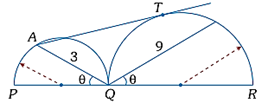
\includegraphics[width=4.5cm]{imagenes/propuestos/geo7.png}
	\end{center}
	
	\begin{enumerate}[label=\alph*)]
		\item $3\sqrt{3}$
		\item 12
		\item 6
		\item 8
		\item 4
	\end{enumerate}
	
	\item En el triángulo mostrado, determina $x$.
	
	\begin{center}
		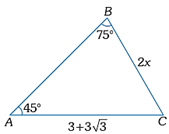
\includegraphics[width=3.5cm]{imagenes/propuestos/geo8.png}
	\end{center}
	
	\begin{enumerate}[label=\alph*)]
		\item $\sqrt{3}$
		\item 3
		\item 2
		\item $\sqrt{3}+1$
		\item $1+\sqrt{6}$
	\end{enumerate}
	
	\item Indicar el valor de verdad de las siguientes proposiciones:
	
	$(\ )$ El seno es creciente en el II C\\
	$(\ )$ El coseno es creciente en el III C\\
	$(\ )$ La tangente es decreciente en el IV C
	
	\begin{enumerate}[label=\alph*)]
		\item V V F
		\item V F V
		\item F F V
		\item F V F
		\item F V V
	\end{enumerate}
	
	\item Si $\tan^2 x+\cot^2 x=2$, donde $x$ pertenece al cuarto cuadrante, halle el valor de:
	
	$U=\dfrac{\cot^{21}x+\tan^{31}x+6}{\tan^{11}x+\cot^{13}x+3}$
	
	\begin{enumerate}[label=\alph*)]
		\item 8
		\item 4
		\item $-4$
		\item 1
		\item 3
	\end{enumerate}
	
	\item La intensidad de corriente que circula por un conductor es de $2\ \mu A$. ¿Qué tiempo demorarán $5\times 10^{13}$ electrones en cruzar una determinada sección transversal del conductor?
	\begin{enumerate}[label=\alph*)]
		\item 1 s
		\item 2 s
		\item 3 s
		\item 4 s
		\item 5 s
	\end{enumerate}
	
	\item El sistema dinámico mostrado en la figura acelera uniformemente tal que el péndulo de masa $m$ se mantiene en equilibrio. Determinar la aceleración de dicho sistema. $(g=10,0\ \text{m/s}^2)$
	
	\begin{center}
		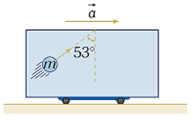
\includegraphics[width=3.5cm]{imagenes/propuestos/fi8.png}
	\end{center}
	
	\begin{enumerate}[label=\alph*)]
		\item 1,0 m/s$^{-2}$
		\item 5,8 m/s$^{-2}$
		\item 9,6 m/s$^{2}$
		\item 10,0 m/s$^{-2}$
		\item 13,3 m/s$^{2}$
	\end{enumerate}
	
	\item En una fábrica se embotella oxígeno gaseoso $(O_2)$ a $27^\circ C$ y 60 atmósferas en cilindros de 0,82 L. Determine la masa del oxígeno que va en los cilindros.
	\begin{enumerate}[label=\alph*)]
		\item 30 g
		\item 520 g
		\item 64 g
		\item 11,2 g
		\item 300 g
	\end{enumerate}
	
	\item Determine la cantidad de calor necesario que se debe suministrar a 500 g de hielo que se encuentra a $0^\circ C$ para convertirlos en agua a $20^\circ C$.
	\begin{enumerate}[label=\alph*)]
		\item 60 kcal
		\item 55 kcal
		\item 50 kcal
		\item 80 kcal
		\item 70 kcal
	\end{enumerate}
	
	\item Una de las alternativas se encuentra entre los oligosacáridos:
	\begin{enumerate}[label=\alph*)]
		\item Quitobiosa
		\item Galactosa
		\item Ribosa
		\item Eritrosa
		\item Xilosa
	\end{enumerate}
	
	\item En la intoxicación por monóxido de carbono, una concentración de carboxihemoglobina de 10 a 20\% produce:
	\begin{enumerate}[label=\alph*)]
		\item dolor de cabeza.
		\item irritabilidad.
		\item desmayo.
		\item confusión.
		\item Muerte
	\end{enumerate}
	
	\item ¿Qué nombre se les ha dado a las democracias que hacen uso de la tecnología, como el voto electrónico, para consolidarse como tales?
	\begin{enumerate}[label=\alph*)]
		\item Puras
		\item Participativas
		\item Digitales
		\item Representativas
		\item Directas
	\end{enumerate}
	
	\item Identifica las emociones en la siguiente relación:
	
	I. alegría\\
	II. odio\\
	III. miedo\\
	IV. amor
	
	\begin{enumerate}[label=\alph*)]
		\item III - IV
		\item I - II
		\item I - IV
		\item II - III
		\item I - III
	\end{enumerate}
	
	\item Son ríos de Europa que vierten sus aguas al Mar Caspio:
	
	1. Don\\
	2. Volga\\
	3. Onega\\
	4. Ural\\
	5. Loira
	
	Son ciertas:
	\begin{enumerate}[label=\alph*)]
		\item 1, 5 y 4
		\item 1, 3 y 5
		\item 2, 1 y 3
		\item 1 y 3
		\item 2 y 4
	\end{enumerate}
	
	\item Con respecto a la Selva Baja, indique lo correcto.
	\begin{enumerate}[label=\alph*)]
		\item Es el sector más poblado de la Amazonía.
		\item Posee la mayor biodiversidad.
		\item Su clima es templado cálido y húmedo.
		\item Se le conoce como la región de los pongos.
		\item Los ríos la recorren de manera torrentosa.
	\end{enumerate}
	
	\item Un ciudadano venezolano, con residencia prolongada y formal en el Perú, siente que el Estado vulnera sus derechos al impedirle acceder a un cargo en el aparato estatal para el cual se sabe calificado. Habiendo agotado las instancias nacionales de justicia, según la Convención Americana sobre Derechos Humanos, dicho ciudadano, ¿está habilitado para que su caso lo vea la Corte Interamericana de Derechos Humanos?
	\begin{enumerate}[label=\alph*)]
		\item No, debido a que Venezuela se apartó de la Convención Americana sobre Derechos Humanos en 2012.
		\item Sí, debido a que el Perú está adscrito a la Convención Americana sobre Derechos Humanos.
		\item Sí, siempre que la Comisión Interamericana de Derechos Humanos asuma su caso como propio.
		\item No, porque dicho ciudadano no ha acatado lo dispuesto por las instancias internas de justicia.
		\item Sí, en la medida que dicho ciudadano haya tramitado oportunamente su nacionalidad peruana.
	\end{enumerate}
	
	
		\item Son tributos administrados por los gobiernos locales.
	
	1. alcabala\\
	2. impuesto general a las ventas\\
	3. impuesto selectivo al consumo\\
	4. predial\\
	5. arbitrios
	
	Son ciertas:
	\begin{enumerate}[label=\alph*)]
		\item 1, 2 y 3.
		\item 1, 3 y 4.
		\item 1, 4 y 5.
		\item 2, 3 y 5.
		\item 3, 4 y 5.
	\end{enumerate}
	
	\item Las funciones que debe cumplir el dinero son:
	
	1. unidad de cuenta\\
	2. medio de pago\\
	3. durabilidad\\
	4. depósito de valor\\
	5. manuabilidad
	
	Son ciertas:
	\begin{enumerate}[label=\alph*)]
		\item 1, 2 y 3
		\item 1, 2 y 4
		\item 1, 2 y 5
		\item 2, 3 y 4
		\item 3 y 5
	\end{enumerate}
	
	\item Durante la época inca, las mujeres escogidas por su belleza física y sus habilidades para el tejido eran conocidas como:
	\begin{enumerate}[label=\alph*)]
		\item illapas
		\item tumipancas
		\item quillas
		\item acllas
		\item pariacacas
	\end{enumerate}
	
	\item La estrategia económica de Estados Unidos para promover el financiamiento, la reconstrucción y reactivación económica de los países de Europa occidental después de la II guerra mundial se denominó:
	\begin{enumerate}[label=\alph*)]
		\item Plan Dodge
		\item Plan Marshall
		\item Alianza para el Progreso
		\item OTAN
		\item Plan Roosevelt
	\end{enumerate}
	
	
	
	
	\item Identifica al filósofo italiano que creó el concepto de “hegemonía cultural”, concepto muy usado actualmente.
	\begin{enumerate}[label=\alph*)]
		\item Antonio Gramsci
		\item Marsilio Ficino
		\item Giambattista Vico
		\item René Descartes
		\item Nicolás de Cusa
	\end{enumerate}
	
	\item En “El banquete”, luego de la conversación con el presidente, a Don Fernando se le prometen dos cosas:
	
	1. una embajada en París\\
	2. asistir, citado él también, al día siguiente a la reunión de diputados\\
	3. una embajada en Roma\\
	4. Don Fernando citará a todos sus ministros para el tema acordado\\
	5. la embajada de Italia y arreglar los caminos a su tierra
	
	Son ciertas:
	\begin{enumerate}[label=\alph*)]
		\item 1 y 2
		\item 1 y 3
		\item 2 y 3
		\item 3 y 4
		\item 4 y 5
	\end{enumerate}
	
	\item En \textit{Cien años de soledad}, y casi al final de la historia, ante los eventos apocalípticos y de destrucción, un fortísimo remolino arrastrará al pueblo hacia la destrucción total, quedando, como testigos y personajes de cierre de estos hechos:
	\begin{enumerate}[label=\alph*)]
		\item Amaranta - José Arcadio
		\item Amaranta Úrsula - Aureliano Babilonia
		\item Rebeca - José Arcadio
		\item Amaranta -- Úrsula
		\item Aureliano Babilonia - Pilar Ternera
	\end{enumerate}
	
	\item Determine el valor de $x$ en la siguiente sucesión numérica:
	
	$1;\ 5;\ 12;\ 25;\ 47;\ 81;\ x$
	
	\begin{enumerate}[label=\alph*)]
		\item 124
		\item 130
		\item 128
		\item 126
		\item 132
	\end{enumerate}
	
	\item Si el ayer de mañana de hace un día fue domingo, ¿qué día será el pasado mañana del mañana del ayer de mañana?
	\begin{enumerate}[label=\alph*)]
		\item Sábado
		\item Lunes
		\item Martes
		\item Viernes
		\item Jueves
	\end{enumerate}
	
	\item Marcar la oración redundante con respecto a la coherencia del texto sobre García Márquez.
	\begin{enumerate}[label=\alph*)]
		\item V
		\item IV
		\item III
		\item II
		\item I
	\end{enumerate}
	
	\item Completar la siguiente oración:
	
	\_\_\_\_\_\_\_ una buena educación el país no progresará.
	
	\begin{enumerate}[label=\alph*)]
		\item Según
		\item Bajo
		\item Sin
		\item Mediante
		\item Tras
	\end{enumerate}
	
	\item ¿Iman allin uywa warmikunaqa llaqtapi kachkan?
	\begin{enumerate}[label=\alph*)]
		\item Puma
		\item Llama
		\item Kuntur
		\item Atoq
		\item Qhari
	\end{enumerate}
	
	\item ¿Mayqinqa verbomi?
	\begin{enumerate}[label=\alph*)]
		\item Wasi
		\item Mikuy
		\item Ñawi
		\item Qocha
		\item Siki
	\end{enumerate}
	

	
	\item The book is \_\_\_\_\_\_\_ the table.
	\begin{enumerate}[label=\alph*)]
		\item behind
		\item under
		\item above
		\item over
		\item all are correct
	\end{enumerate}
	
	\item She said, “I am tired.” $\rightarrow$ She said that she \_\_\_ tired.
	\begin{enumerate}[label=\alph*)]
		\item is
		\item was
		\item were
		\item be
		\item had been
	\end{enumerate}
	
\end{enumerate}


\subsubsection*{Claves de Respuestas}

\begin{center}
	\begin{tabular}{ll ll ll ll ll ll}
		1) E & 2) A & 3) E & 4) D & 5) C & 6) B \\
		7) B & 8) B & 9) D & 10) E & 11) C & 12) C \\
		13) A & 14) A & 15) C & 16) E & 17) E & 18) B \\
		19) B & 20) B & 21) D & 22) B & 23) A & 24) C \\
		25) B & 26) B & 27) E & 28) B & 29) C & 30) B \\
		31) B & 32) E & 33) B & 34) B & & \\
	\end{tabular}
\end{center}



	

\end{document}
